\documentclass[a4paper, 12pt]{report}
\usepackage{hyperref}
\usepackage{gensymb}
\usepackage{ amssymb }
\usepackage[utf8]{inputenc} % выбор кодировки кода
\usepackage[T2A]{fontenc} % выбор внутренней кодировки 
\usepackage[english, russian]{babel} % выбор языка
% \righthyphenmin = 2 % минимальное число букв после переноса: может пригодиться
\usepackage{multirow}
\usepackage{fontawesome}
\usepackage{easyReview}
\usepackage{tabularx}
\usepackage{rotating}
\usepackage{amsmath} % русский текст в формулах
\usepackage{color} % цвет текста
\usepackage{ulem} % для зачёркивания текстаё

\usepackage[left=15mm, right=10mm, top=20mm, bottom=20mm]{geometry} % поля
\usepackage{indentfirst} % отступ первого абзаца
\setlength{\parindent}{1,25cm} % длина отступа первой строки абзаца
\linespread{1,5} % междустрочный интервал

\usepackage{titlesec} % настройка заголовков
\renewcommand{\thesection}{\arabic{section}} % противотараканная мера для report'а: делаю section заголовком первого уровня
\titleformat{\section}{\centering \large \bfseries}{\thesection}{1ex}{\MakeUppercase}{}
\titleformat{\subsection}{\centering \large \bfseries}{\thesubsection}{1ex}{}{}
\titleformat{\subparagraph}[runin]{\bfseries}{\thesubparagraph}{}{}{}

% \titleformat{\bibliography}{\centering \large \bfseries}{\thebibliography}{}{}{} % попытка настроить заголовок для списка литературы

\usepackage{graphicx}
\graphicspath{{./Photos/}}


\usepackage{comment} % Для многострочных комментариев
\usepackage{xcolor} % Для девочек 
\usepackage{enumitem}

\usepackage[
natbib		= true,
style		= gost-numeric,
sorting		= none,
backend		= biber,
language	= autobib,
bibstyle	= gost-numeric,
citestyle	= gost-numeric,
autolang	= other]{biblatex}
\addbibresource{Gvandra2024_biblio.bib}

\begin{document}
\begin{titlepage}
\setlength\parindent{0pt}
	\begin{center}
		\large{РОО <<Федерация спортивного туризма Московской области>>\\
		ОО г. Долгопрудного <<Федерация спортивного туризма>>\\}
	\end{center}

	


	
	\begin{center}
		
\includegraphics[width=0.4\linewidth]{../pics/Flag_GS-2}
		
		\Large{\bfseries{ОТЧЁТ}} \\
		\normalsize о прохождении горного спортивного туристического маршрута \textbf{первой} категории сложности по Западному Кавказу (Гвандра), совершённом с 18 по 30 августа 2024 г. группой туристов Горной секции МФТИ ФСТ Московской области, г. Долгопрудный
	\end{center}
	\vspace{1.5 cm}
	
	\textbf{Маршрутная книжка:} 41/2024, выдана МКК ФСТ МО г. Долгопрудный \\ 
	\textbf{Руководитель группы:} Снеговская Дарья Алексеевна\\
	\textbf{E-mail:} \href{mailto: snegovskaya\_da@mail.ru}{snegovskaya\_da@mail.ru}\\
	\textbf{Номер телефона:} $+7(964)599-90-08$
	
	\vspace{0.2cm}
	
	\textit{Маршрутно-квалификационная комиссия Федерации спортивного туризма Московской области рассмотрела отчёт и считает, что маршрут может быть зачтен всем участникам и руководителю \textbf{первой категории сложности}.}

	\vspace{0.2cm}
	
	Отчёт использовать в библиотеке ФСТ Московской области и ФСТ г. Долгопрудный.
	
	\vspace{1cm}
	
	\textbf{Судья по виду:}
	
	\vspace{0.5cm}
	\textbf{Председатель МКК:}
	
	\vspace{1cm}
	\textbf{Штамп МКК:}
	
	\vfill
	\begin{center}
		Долгопрудный,   \the\year{}
	\end{center}
\end{titlepage}

\renewcommand{\contentsname}{Содержание}
\tableofcontents
\clearpage
\section*{Сокращения, используемые в отчёте}
\addcontentsline{toc}{section}{Сокращения, используемые в отчёте}
\begin{tabular}{p{0.08\textwidth} p{0.7\textwidth}}
	МКК                                  &   Маршрутно-квалификационная комиссия  \\
	ФСТ                                &   Федерация спортивного туризма  \\
	к.с.                               &   категория сложности (похода)  \\
	ст.с.							& степень сложности (похода) \\
	н/к                            &   некатегорированный (перевал, препятствие) \\
	орогр.                &   орографически  \\
	ЧХВ                          &   чистое ходовое время  \\
	т/б                         &   туристическая база \\
	т/к                         &   туристический клуб \\
	а/л                  &   альпинистский лагерь \\
		с. & село \\
	г. & город \\
	ст. & станция (канатной дороги) \\
	верш.               &   вершина \\
	пер.               &   перевал \\
	оз.             &   озеро \\
	р.             &   река \\
	д.	&	долина\\
	хр. &   хребет \\
	тр. &   травянистый \\
	ос. &   осыпной \\
	ск. &   скальный \\
	сн. &   снежный \\
	лед. &   ледовый \\
	лев. &   левый \\
	пр. &   правый \\
	пхд	&	по ходу движения	\\
	рук. &   руководитель \\	
	КЧР & Карачаево-Черкесская республика\\
	КБР & Кабардино-Балкарская республика\\
	ГКХ	&	Главный Кавказский хребет \\
	м.н. & место ночёвки
\end{tabular}
\clearpage
\section{Справочные сведения о походе} 
\subsection{Проводящая организация}
Поход был совершён в рамках школы горного туризма базового уровня, организованной Горной секцией МФТИ.


\subsection{Место проведения}
\textbf{Страна:} Россия

\textbf{Субъекты федерации:} КЧР, КБР

\textbf{Район:} Западный Кавказ

\textbf{Подрайоны:} Гвандра, Приэльбрусье

\subsection{Общие справочные сведения о маршруте}

\begin{table}[h!]
	\resizebox{\textwidth}{!}{%
		\begin{tabular}{|c|c|c|cc|c|}
			\hline
			\multirow{2}{*}{\begin{tabular}[c]{@{}c@{}}Дисциплина\\ (вид туризма)\end{tabular}} & \multirow{2}{*}{\begin{tabular}[c]{@{}c@{}}Категория сложности\\ маршрута\end{tabular}} & \multirow{2}{*}{\begin{tabular}[c]{@{}c@{}}Протяжённость\\ активной части, км$^1$\end{tabular}} & \multicolumn{2}{c|}{\begin{tabular}[c]{@{}c@{}}Продолжительность активной\\ части\end{tabular}} & \multirow{2}{*}{Сроки проведения}                                   \\ \cline{4-5}
			&                                                                                         &                                                                                             & \multicolumn{1}{c|}{Общая}                            & Ходовых дней                            &                                                                     \\ \hline
			Горный                                                                              & Первая                                                                                  & 111                                                                                         & \multicolumn{1}{c|}{13}                               & 13                                      & \begin{tabular}[c]{@{}c@{}}18.08.2024-\\ 30.08.2024 г.\end{tabular} \\ \hline
		\end{tabular}%
	}
\end{table}
\footnotesize{$^1$ С учётом коэффициента $k=1.2$, без учёта повторно пройденного пути}
\normalsize

\subsection{Подробная нитка маршрута}
\textbf{Заявленная:} г. Минеральные Воды~--- д.р. Учкулан~--- д.р. Кичкинакол Уллукёльский~--- \textbf{пер. Уллукёль Восточный (1А, 3050)}~--- т/б <<Глобус>>~--- д.р.Гондарай~--- д.р. Джалпаккол~--- \textbf{пер. Джалпаккол Сев. (1А, 3400)}~--- д.р. Мырды~--- а/л<<Узункол>>~--- д.р.Кичкинекол~--- д.р. Таллычат~--- \textbf{пер. Кичкинекол Малый (1А, 3210)}~--- д.р. Чунгур-Джар~--- \textbf{пер. Перемётный (1А, 3242)}~--- д.р. Танышхан~--- д.р. Чиринкол~--- стоянка <<Гвандра>>~--- д. р. Кубань~--- \textbf{пер. Хотютау (1А, 3546)}~--- лед. Большой Азау~--- с. Терскол

\textbf{Пройденная:} Маршрут пройден без изменений.

\textbf{Корнилов Георгий} сошёл с маршрута в т/б <<Глобус>>. Он прошёл перевал Уллукёль Восточный (1А$^{\star}$). \alert{L=??}

\textbf{Миронова Наталья} сошла с маршрута в а/л <<Узункол>>. Она прошла перевалы Уллукёль Восточный (1А$^{\star}$), Джалпаккол Северный (1А$^{\star}$). \alert{L=??}

\textbf{Шалфеев Илья, Мерзликина Дарья, Сингалевич Дмитрий, Семено Мария} сошли с маршрута после д.р. Чиринкол, на погранзаставе <<Хурзук>>. Они прошли перевалы Уллукёль Восточный (1А$^{\star}$), Джалпаккол Северный (1А$^{\star}$), Кичкинекол Малый (1А), Перемётный (1А). \alert{L=??}

\begin{figure}
	\centering
	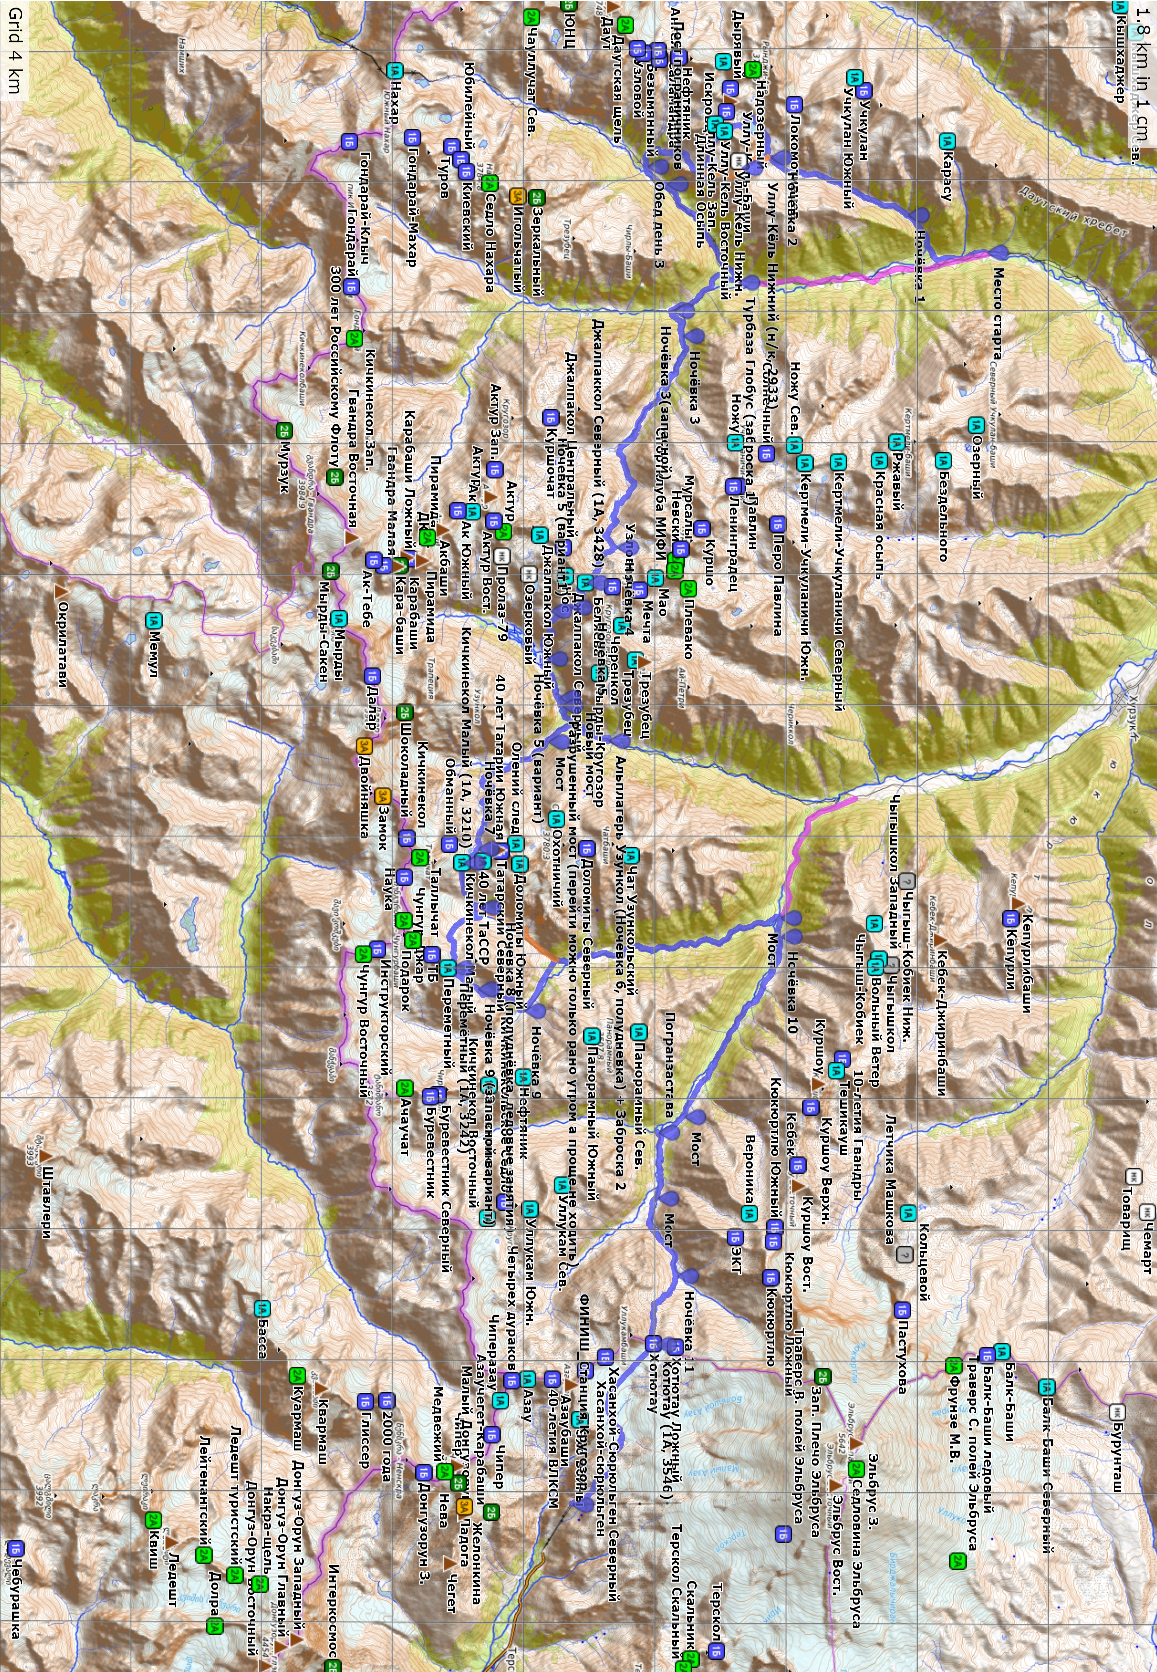
\includegraphics[width=0.92\linewidth]{../pics/map}
	\caption{Обзорная схема маршрута}
\end{figure}
	
\subsection{Высотный профиль маршрута}

\begin{figure}
	\centering
	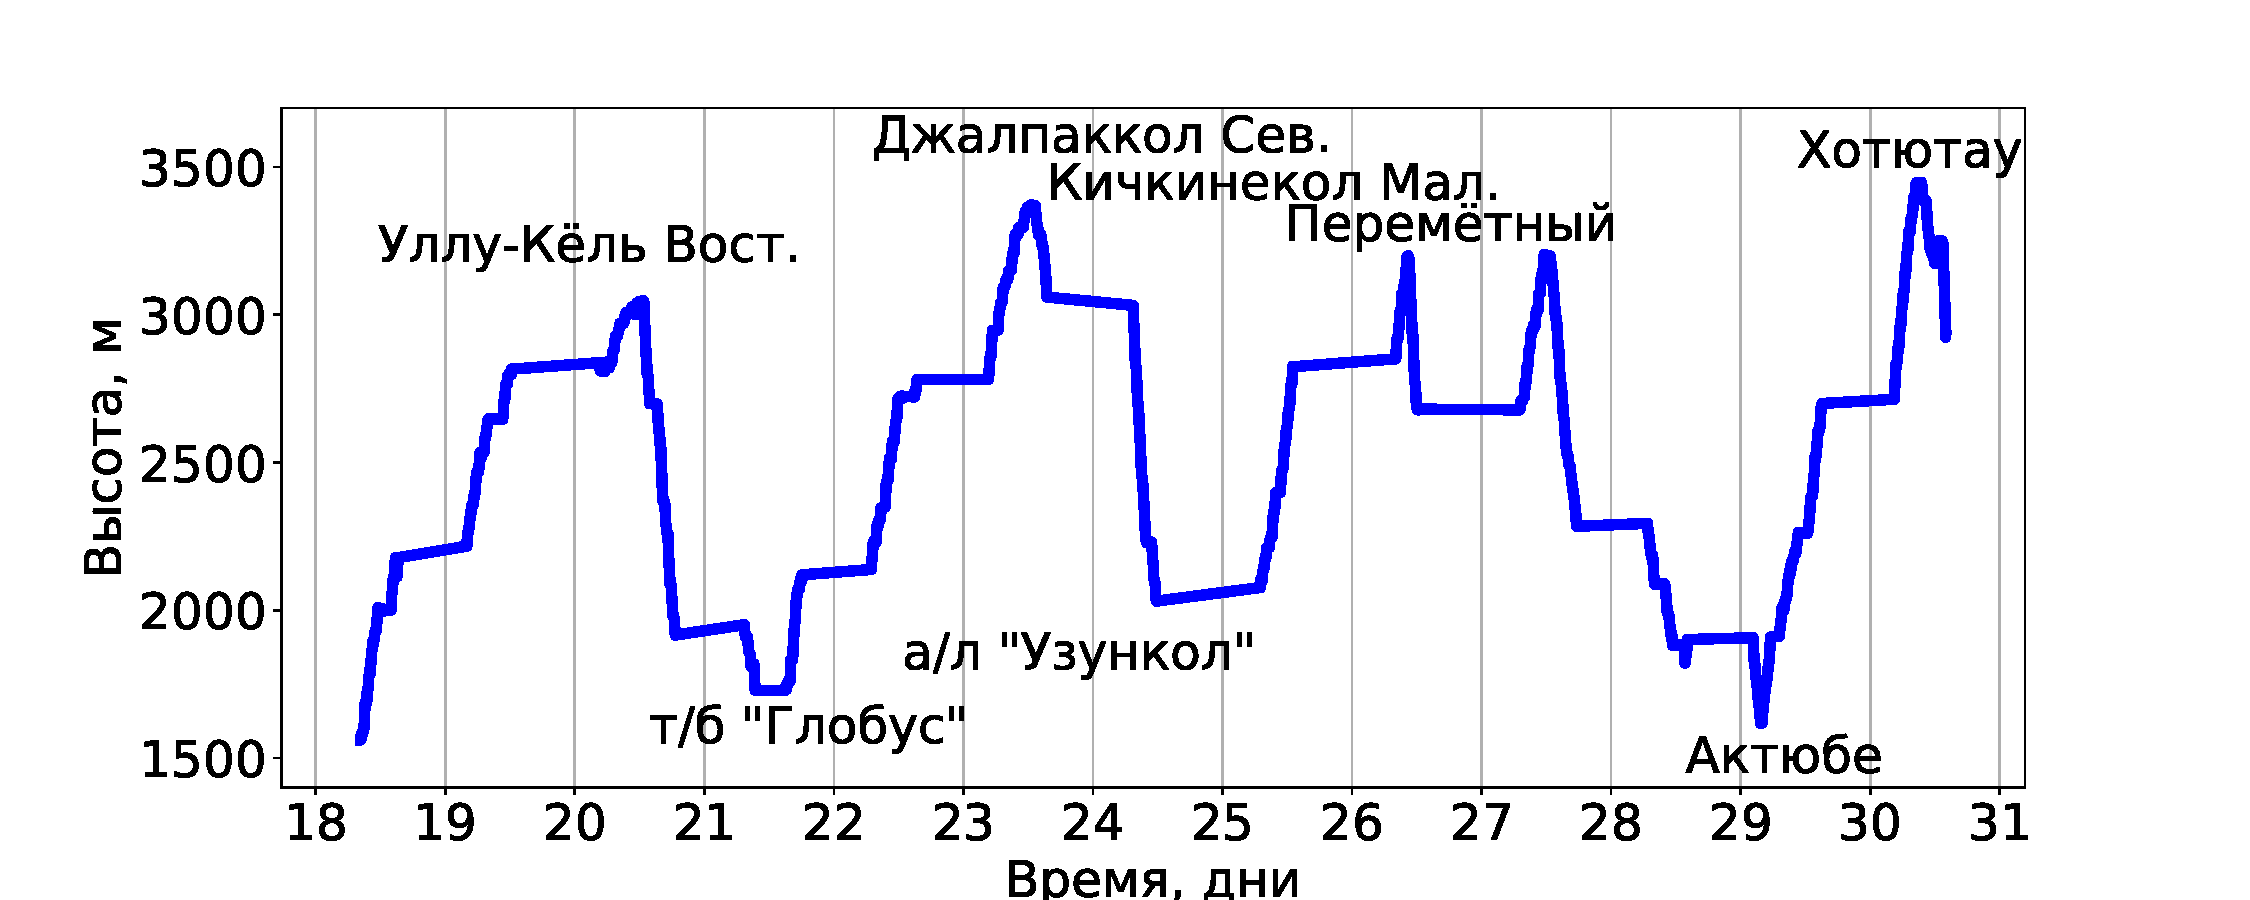
\includegraphics[width=0.92\linewidth]{../pics/elevation_vs_time}
	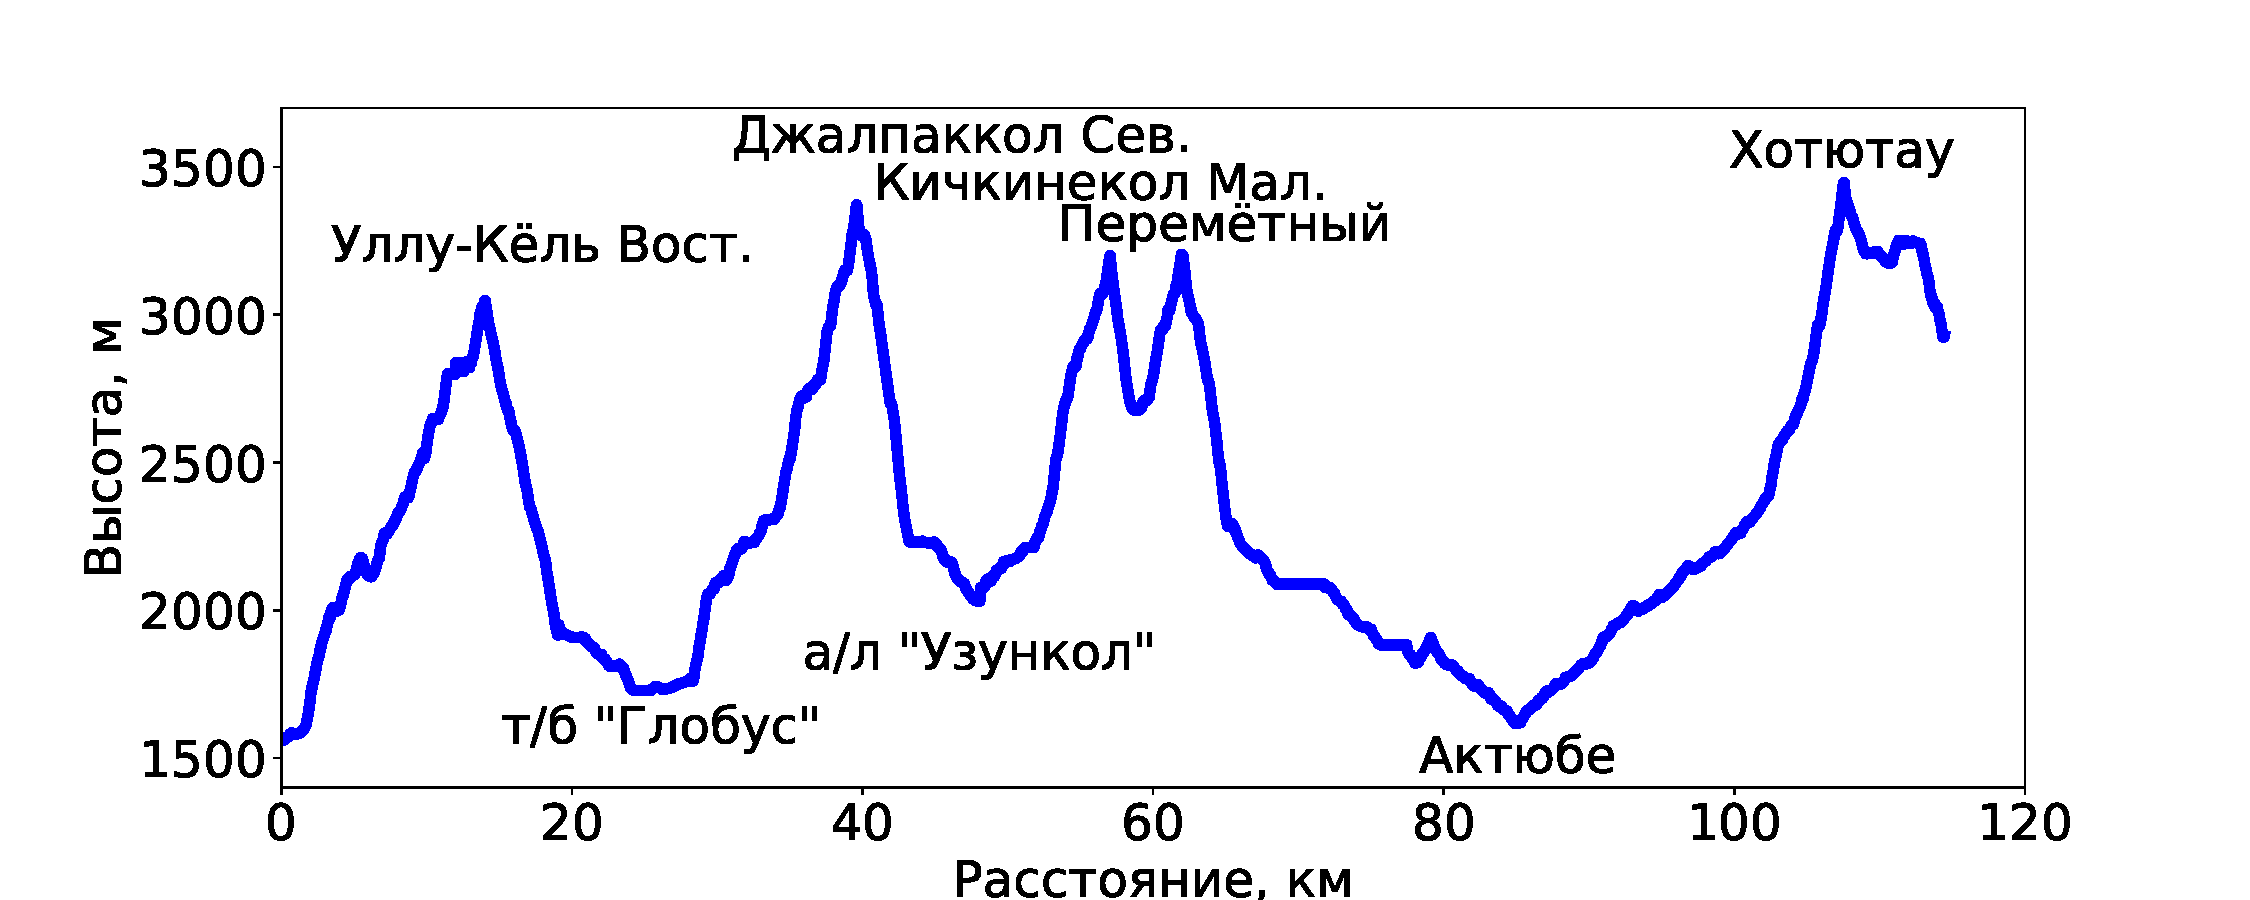
\includegraphics[width=0.92\linewidth]{../pics/elevation_vs_distance}
	\caption{Высотный профиль маршрута}
	\label{fig:heights}
\end{figure}

\subsection{Определяющие препятствия маршрута}

\begin{table}[h!]
		\begin{tabular}{|>{\centering\arraybackslash}m{0.17\linewidth}|>{\centering\arraybackslash}m{0.03\linewidth}|>{\centering\arraybackslash}m{0.4\linewidth}|>{\centering\arraybackslash}m{0.3\linewidth}|}
			\hline
			\textbf{Вид препятствия, высота} &
			\begin{turn}{90}\textbf{к. тр.}\end{turn} &
			\textbf{Характеристика препятствия на подъём} &
			\textbf{Характеристика препятствия на спуск} \\
			\hline			
			пер. Уллу-Кёль Восточный, 3050 & 1А$^{\star}$ &  Со стороны оз. Уллукёль ос. перевальный взлёт протяжённостью до 350 м. У подножия крутизна $20-25^{\circ}$; далее осыпной участок крутизной до $30^{\circ}$ протяжённостью до 100 м и далее снежник крутизной до $35-40^{\circ}$, а в верхней части до $45^{\circ}$, протяжённостью до 50 м. & Движение по гребню до озера под перевалом, далее травяной склон \\
			\hline			
			пер. Джалпаккол Северный, 3411  & 1А$^{\star}$ & Со стороны д.р. Джалпаккол перевальный взлёт лед.-ос. протяжённостью до 200 м, крутизной $35-40^{\circ}$. Выход на перевал — 5 м простого лазания на скальный гребень.  & ск.-ос., протяжённостью до 150 м, крутизной до $30^{\circ}$ \\
			\hline
			пер. Кичкинекол Малый, 3206  & 1А & Со стороны д.р. Кичкинекол по тр.-ос. склону по тропе, протяжённостью до 300 м, крутизной до $25^{\circ}$. На седловине перевала снежник. & ск.-ос. тропа протяжённостью до 200 м., крутизной до $15^{\circ}$\\
			\hline
			пер. Перемётный, 3255  & 1А & Со стороны д.р. Чунгур-Джар перевальный взлёт ск.-ос. протяжённостью до 400 м, крутизной до  $20^{\circ}$ & ск.-ос. склон протяжённостью до 100 м, крутизной до $35^{\circ}$, далее косым траверсом по курумнику. Обход сбросов левее березняка по лощине.\\
			\hline
			пер. Хотютау, 3546  & 1А$^{\star}$ & Со стороны д.р. Уллу-Кам подъём по ос.склону протяжённостью до 1000 м, крутизной до $25^{\circ}$. &  ос. склон протяжённостью до 70 м, крутизной до $30^{\circ}$, выход на открытый ледник\\
			\hline
	\end{tabular}%
\end{table}

\subsection{Список участников} 
Тут будет список наших \sout{долбанов} зайчиков.
\begin{table}[h!]
	\centering
	\resizebox{0.77\textwidth}{!}{%
	\begin{tabular}{|>{\centering\arraybackslash}m{0.02\linewidth}|>{\centering\arraybackslash}m{0.2\linewidth}|>{\centering\arraybackslash}m{0.14\linewidth}|>{\centering\arraybackslash}m{0.05\linewidth}|>{\centering\arraybackslash}m{0.15\linewidth}|>{\centering\arraybackslash}m{0.18\linewidth}|}
		\hline
		\textbf{№} &
		\textbf{Фото} &
		\textbf{ФИО} &
		\textbf{г.р.} &
		\textbf{Обязанности в группе} &
		\textbf{Спортивный опыт} \\
		\hline			
		
		1	&	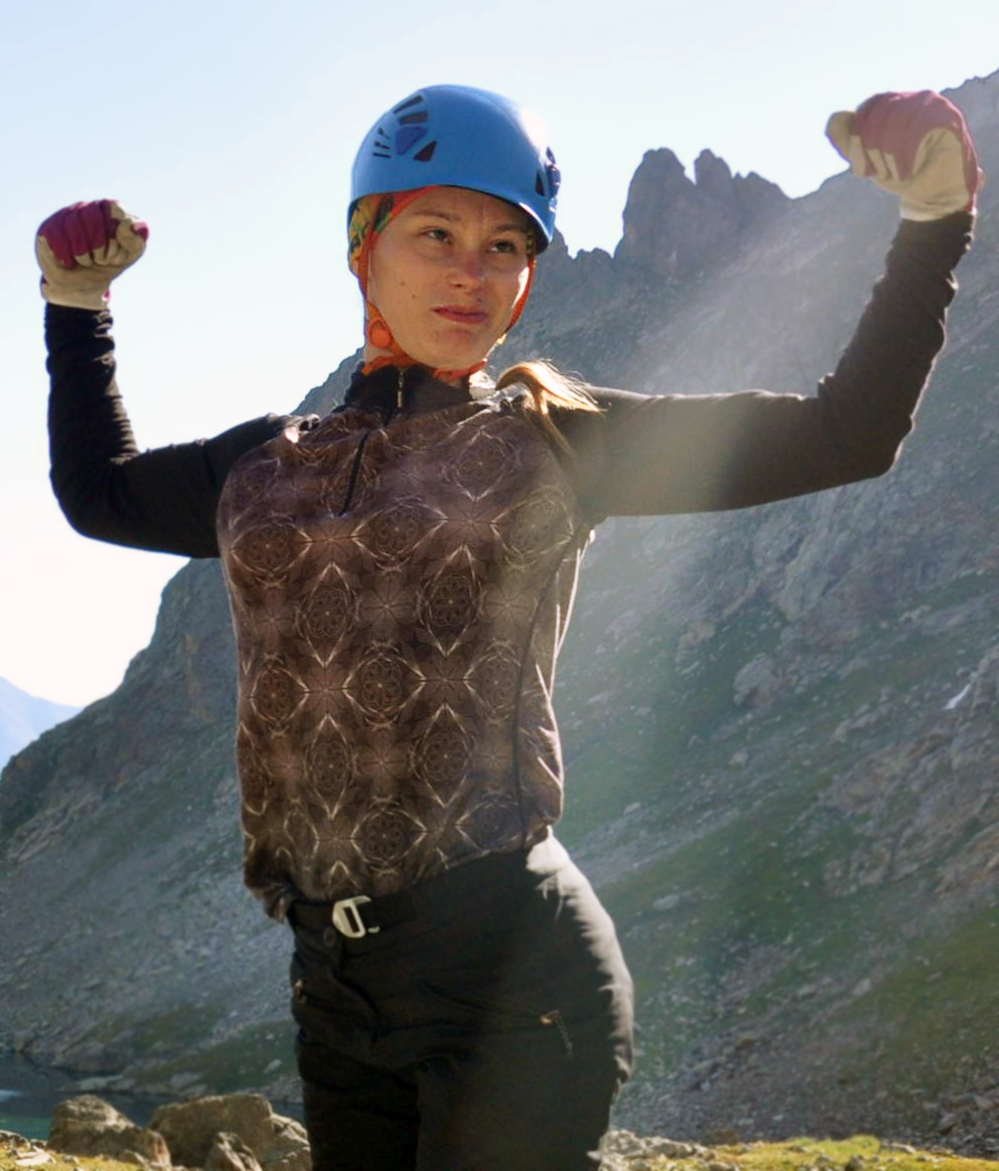
\includegraphics[width=0.99\linewidth]{../pics/portraits/dasha_s.png}	&	Снеговская Дарья Алексеевна	&	1997	&	Руководитель	& 3ГУ, Центральный Кавказ, 2020 \newline 1ГУ, Алтай, Северо-Чуйский хребет, 2023 \\
		\hline
		2	& 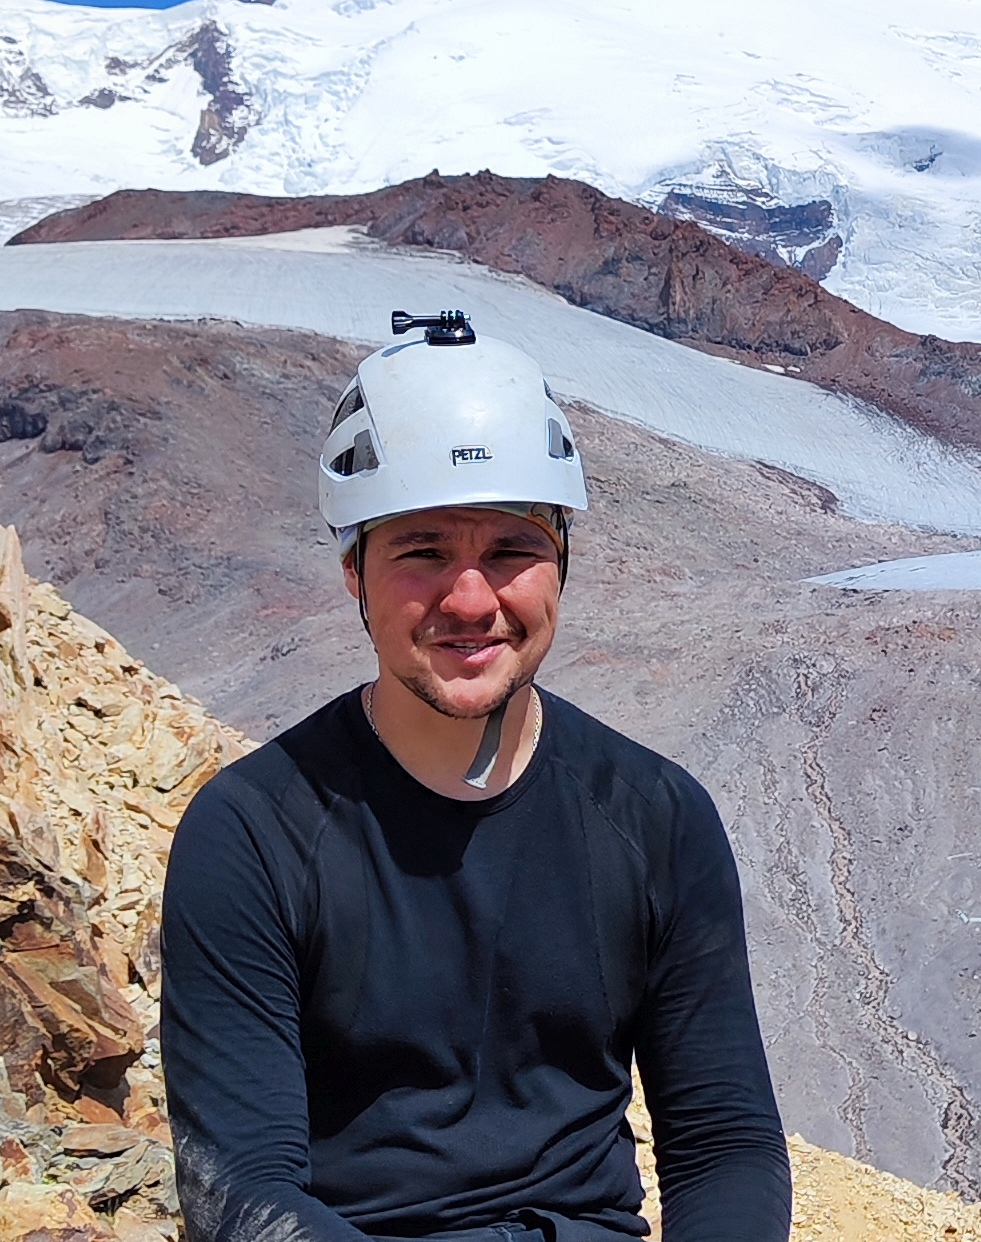
\includegraphics[width=0.99\linewidth]{../pics/portraits/lesha_o1}	&	Остапив Алексей Юрьевич	&	1998	&	Зам. руководителя	& 2ГУ, Киргизский хребет, 2019 \newline 1ГУ, Алтай, Северо-Чуйский хребет, 2023 \\
		\hline
		3	&	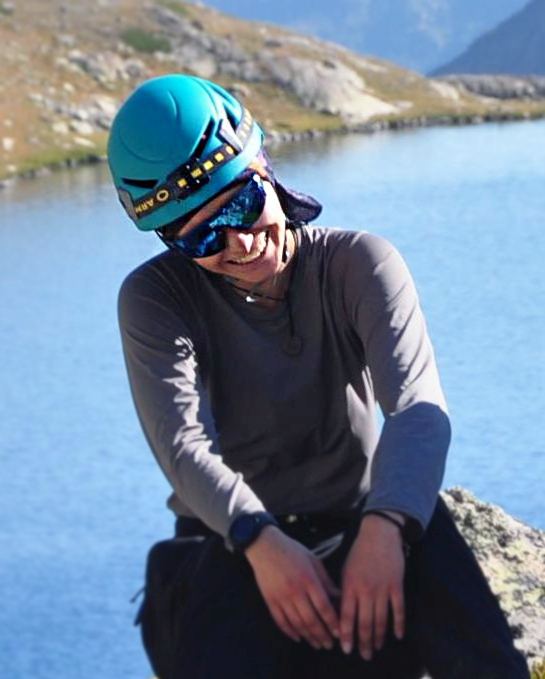
\includegraphics[width=0.99\linewidth]{../pics/portraits/katya}	&	Тюрина Екатерина Алексеевна	&	2004	&	Медик	&	1 ст.с. \\
		\hline
		4	&		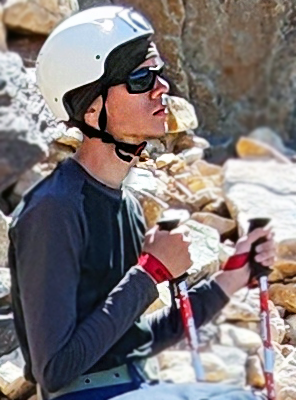
\includegraphics[width=0.99\linewidth]{../pics/portraits/dima_d.png}		&	Дёмушкин .Дмитрий Юрьевич	&	2001	&	Штурман	&	1 ст.с. \\
		\hline
		5	&	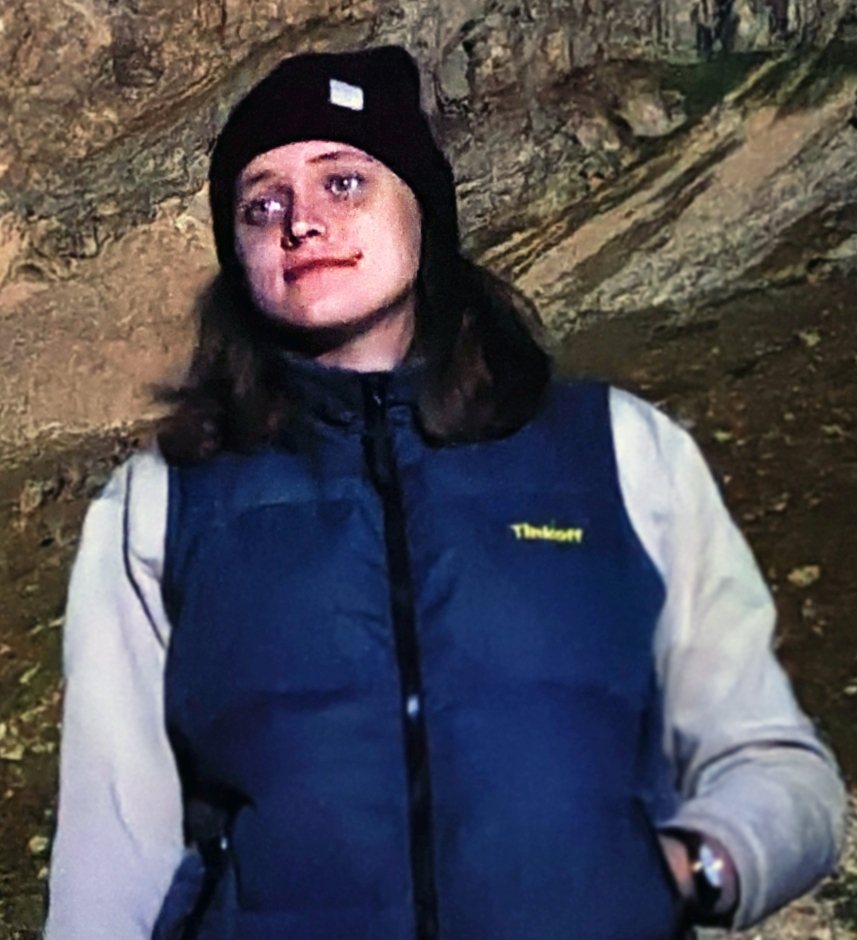
\includegraphics[width=0.99\linewidth]{../pics/portraits/natasha}	&	Миронова Наталья Сергеевна	&	2000	&	Хронометрист	&	1 ст.с. \\
		\hline
		6	&	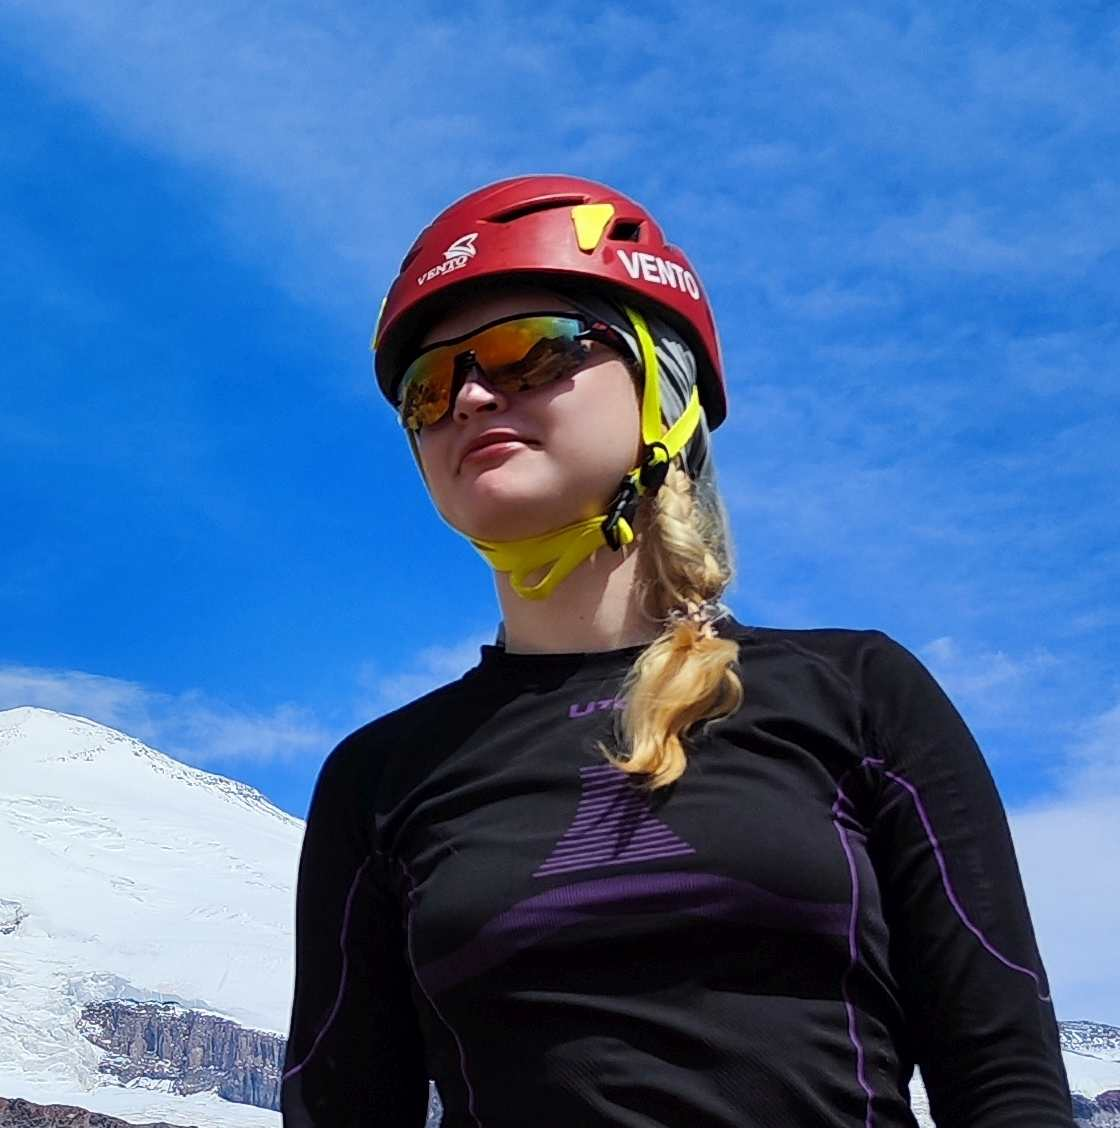
\includegraphics[width=0.99\linewidth]{../pics/portraits/dasha_k}	&	Казаринова Дарья Дмитриевна	&	2001	&	Логист	&	1 ст.с. \\
	\hline
	\end{tabular}%
	}
\end{table}


\begin{table}[h!]
	\centering
	\resizebox{0.75\textwidth}{!}{%
	\begin{tabular}{|>{\centering\arraybackslash}m{0.02\linewidth}|>{\centering\arraybackslash}m{0.2\linewidth}|>{\centering\arraybackslash}m{0.14\linewidth}|>{\centering\arraybackslash}m{0.05\linewidth}|>{\centering\arraybackslash}m{0.15\linewidth}|>{\centering\arraybackslash}m{0.18\linewidth}|}
		\hline
		\textbf{№} &
		\textbf{Фото} &
		\textbf{ФИО} &
		\textbf{г.р.} &
		\textbf{Обязанности в группе} &
		\textbf{Спортивный опыт} \\
		\hline
		7	&	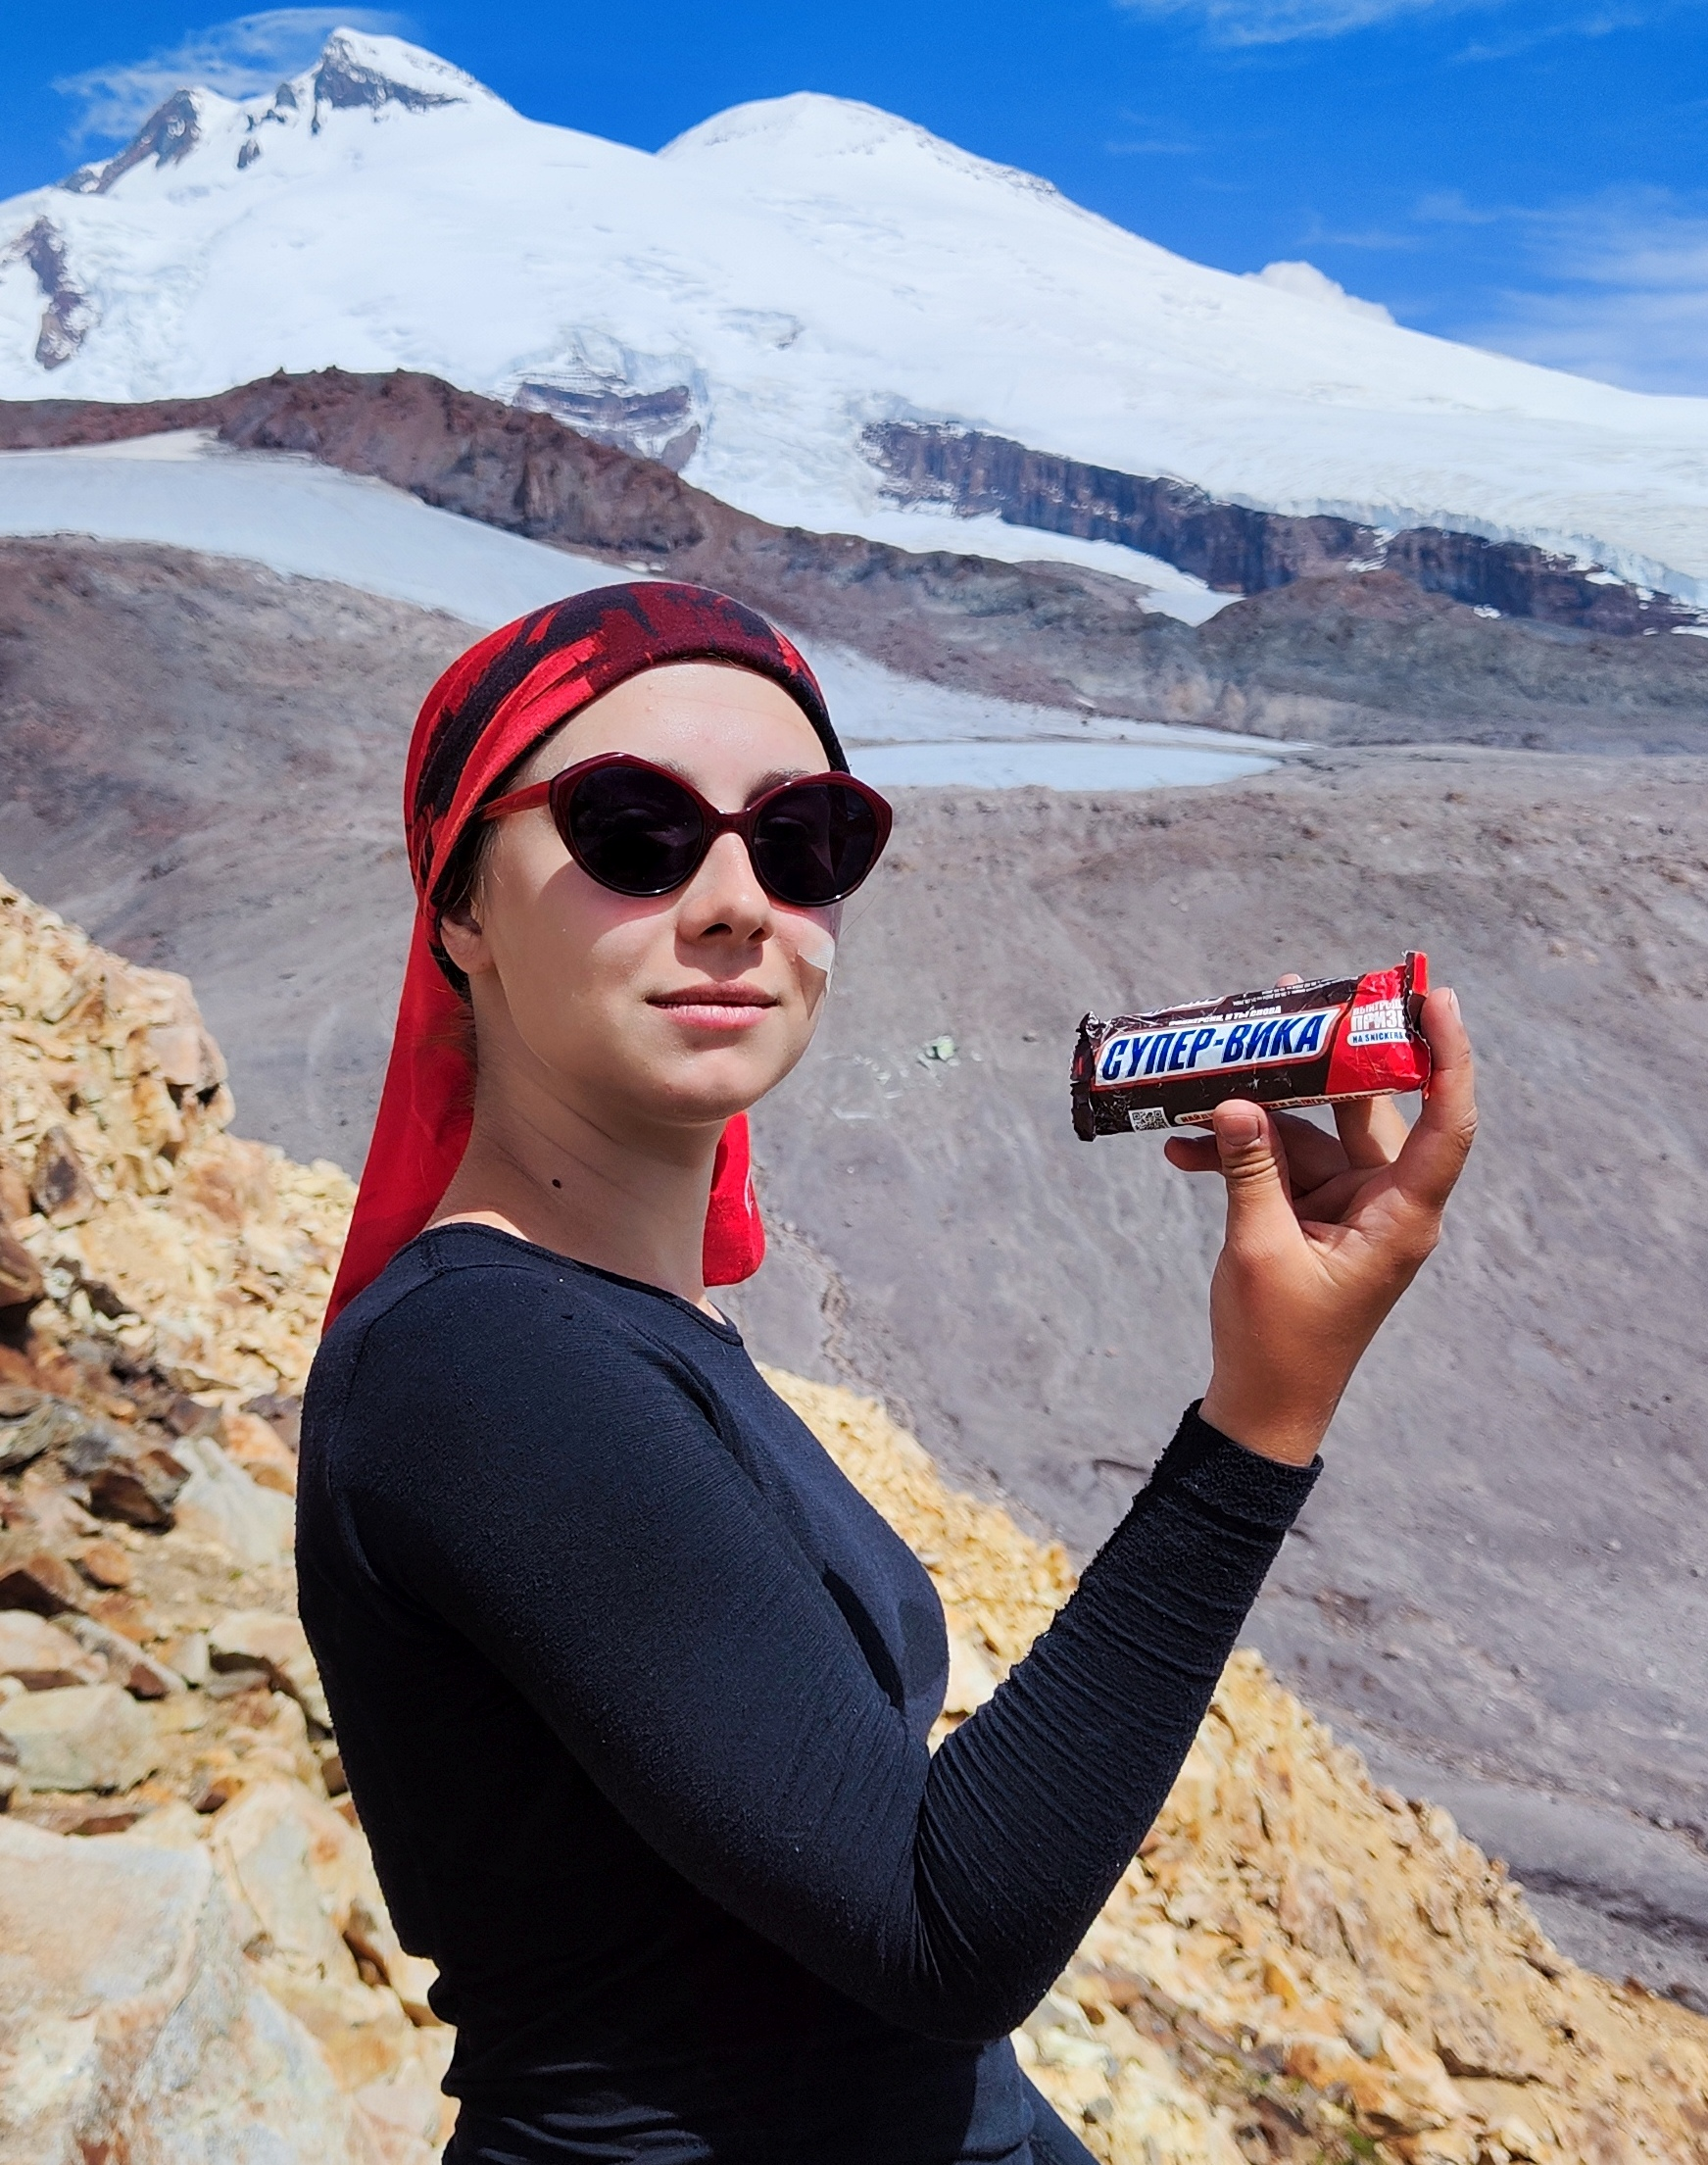
\includegraphics[width=0.99\linewidth]{../pics/portraits/vika}	&	Суровцева Виктория Павловна	&	2002	&	Снаряженец	&	1 ст.с. \\
		\hline
		8	&	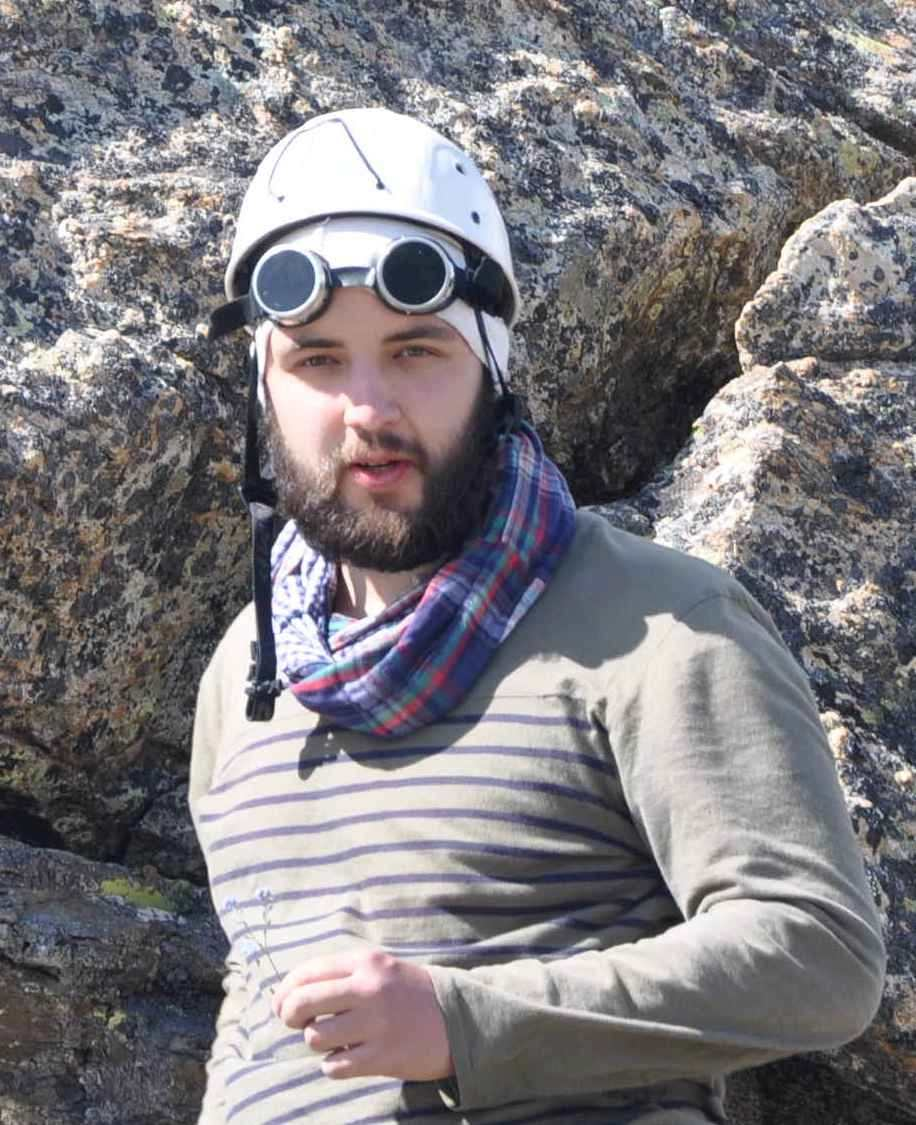
\includegraphics[width=0.99\linewidth]{../pics/portraits/gosha}		&	Корнилов Георгий Алексеевич	&	2003	&	Завхоз 1	&	1 ст.с. \\
		\hline
		9	&	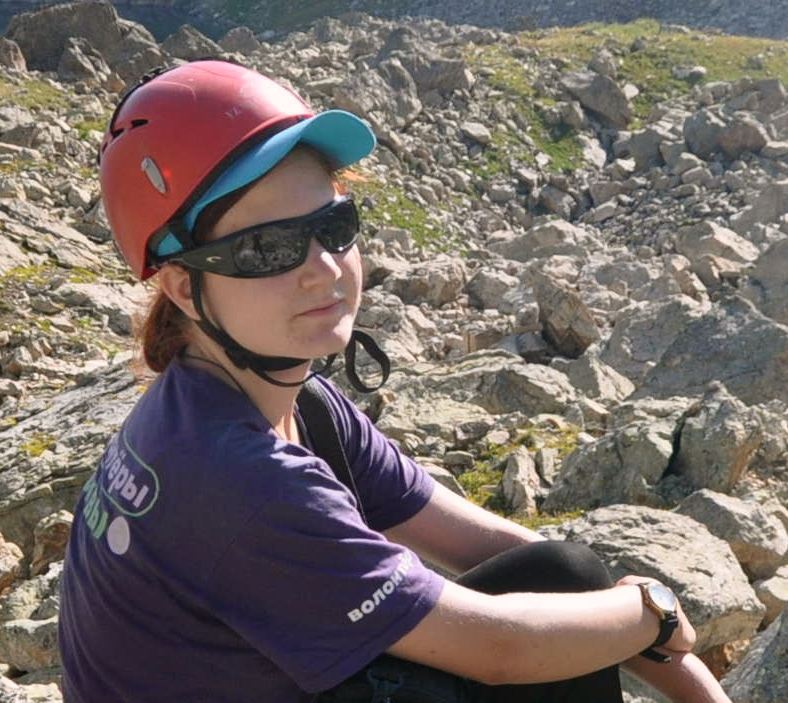
\includegraphics[width=0.99\linewidth]{../pics/portraits/masha}	&	Семено Мария Алексеевна	&	2006	&	Завхоз	2	&	1 ст.с. \\
		\hline
		10	&	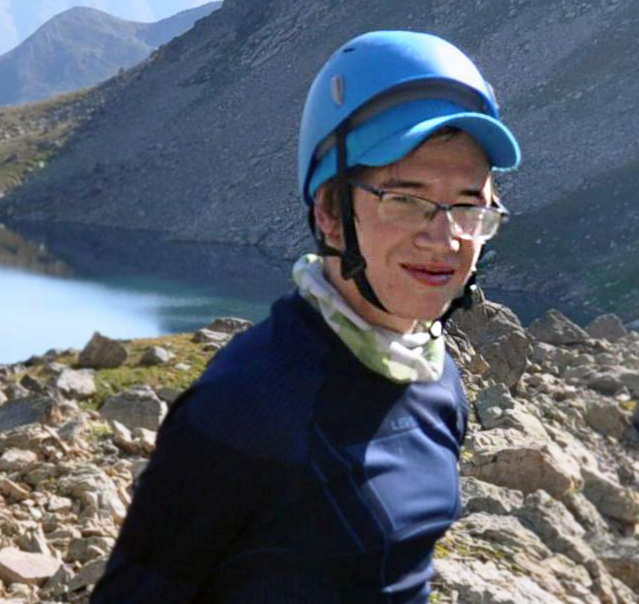
\includegraphics[width=0.99\linewidth]{../pics/portraits/dima_s}	&	Сингалевич Дмитрий Константинович	&	2004	&	Эколог	&	1 ст.с. \\
		\hline
		11	&	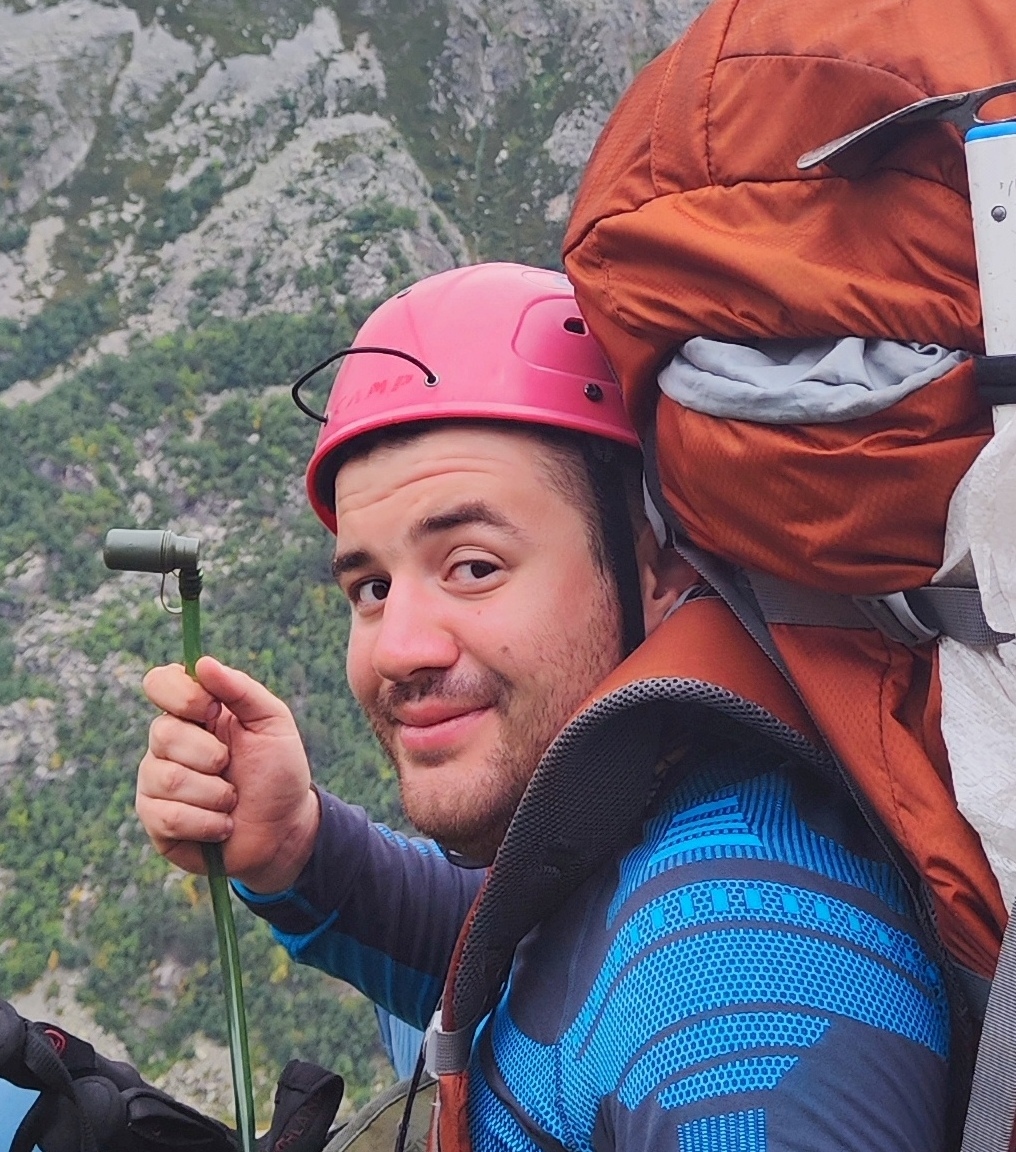
\includegraphics[width=0.99\linewidth]{../pics/portraits/ilya_sh}	&	Шалфеев Илья Андреевич	&	1997	&	Финансист	&	1 ст.с. \\
		\hline
		12	&	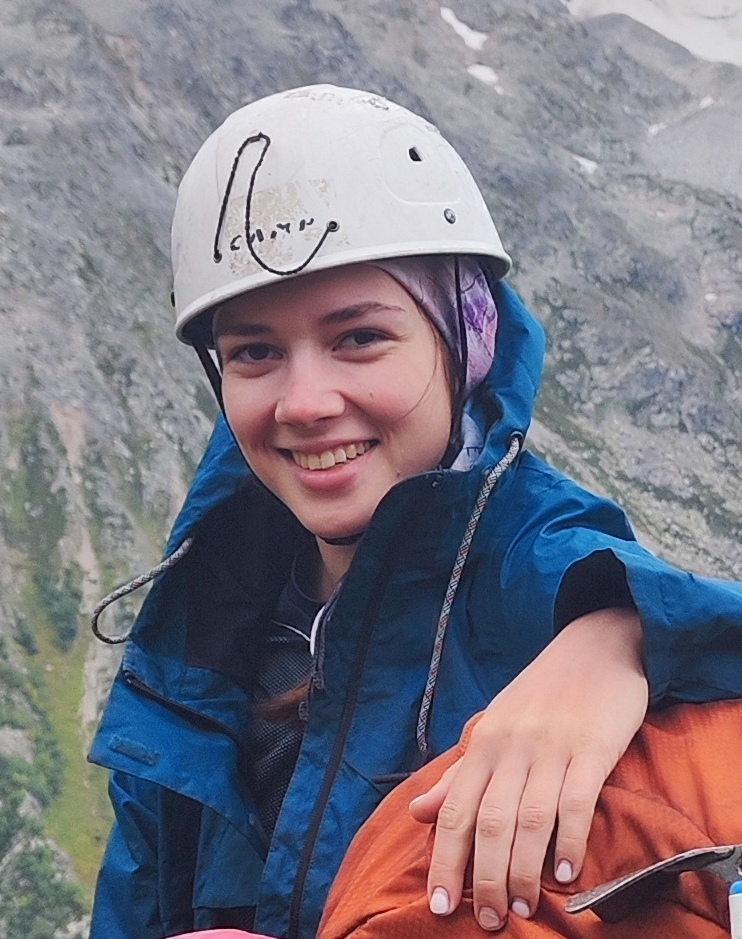
\includegraphics[width=0.99\linewidth]{../pics/portraits/dasha_m}	&	Мерзликина Дарья Сергеевна	&	2000	&	Реммастер	&	1 ст.с. \\
		\hline
		12$^\star$	&	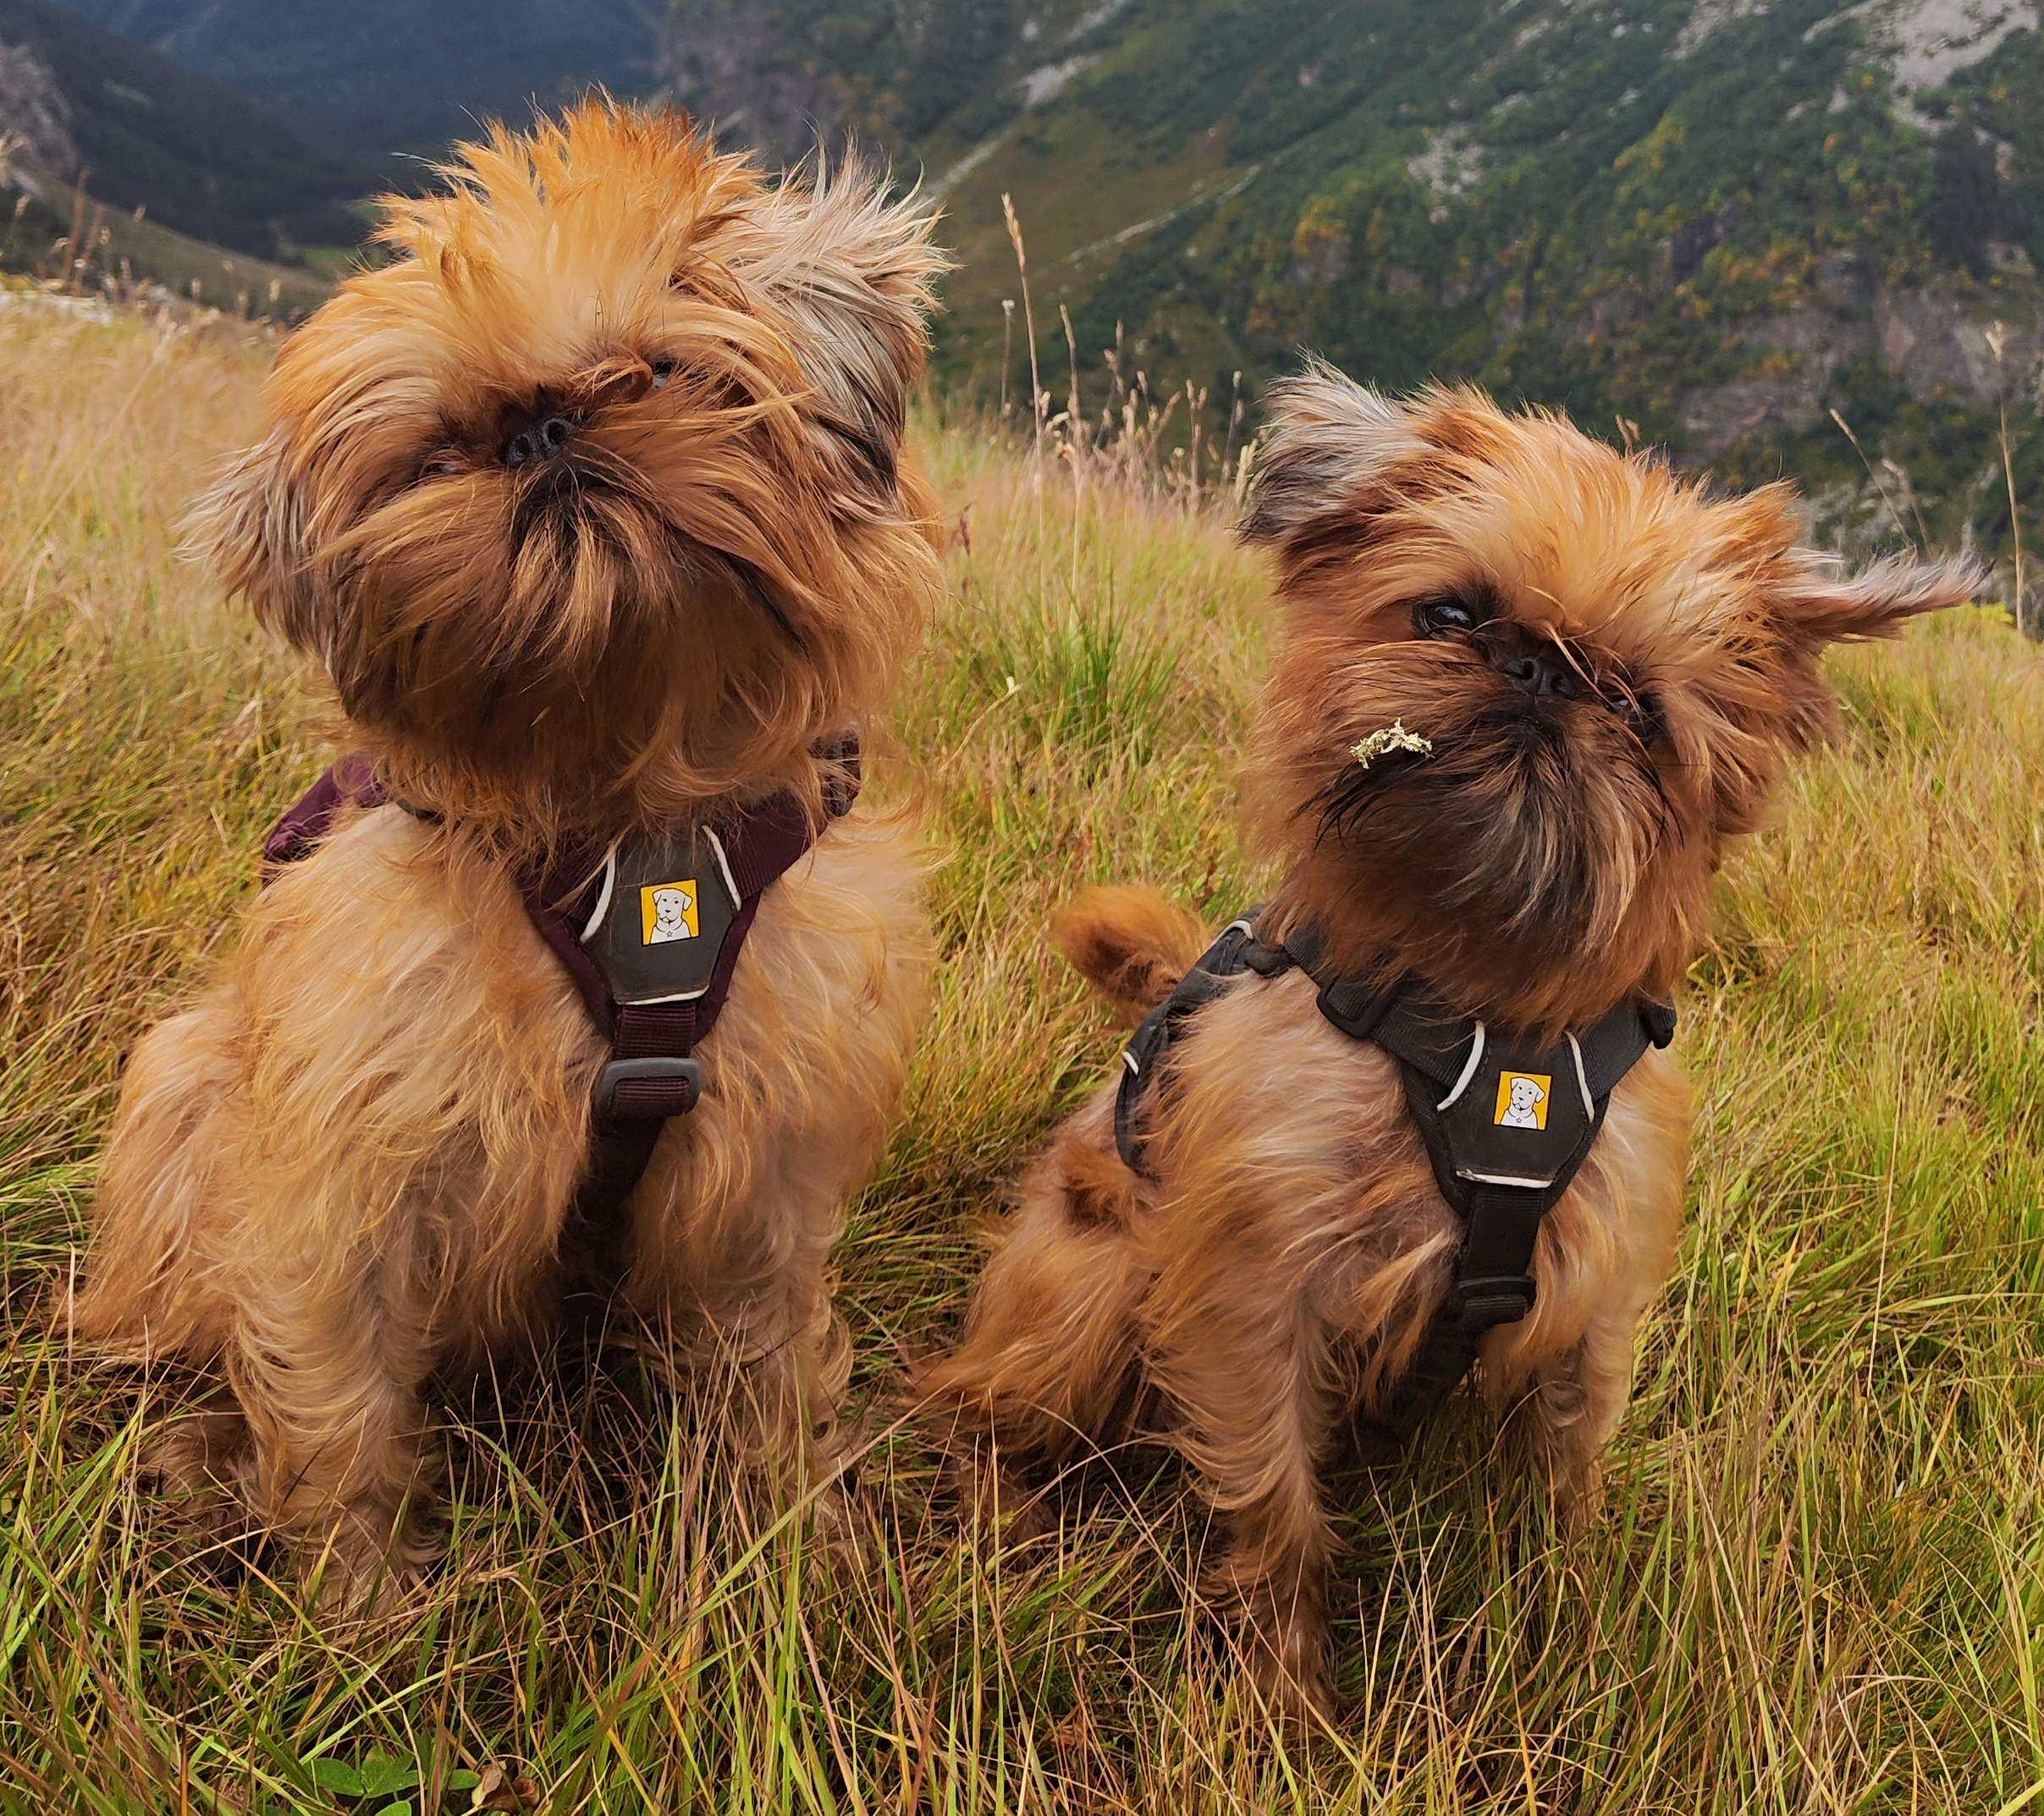
\includegraphics[width=0.8\linewidth]{../pics/portraits/yoshta_aina}	&	Йошта, Айна (брюссельские гриффоны)	&	2022	&	Талисманы команды	&	1 ст.с. \\
		\hline
	\end{tabular}%
	}
\end{table}


%\newpage
\section{Организация и проведение похода}
\subsection{Цели и задачи маршрута. Выбор нитки маршрута}
При места проведения маршрута в целом, я как руководитель опиралась на следующие соображения: 
\begin{enumerate} 
	\item \textbf{Транспортная доступность горного района и стоимость трансфера.}
	Поскольку группа, как и планировалось, практически полностью состояла из новичков, в этом случае особенно важно было затратить минимум сил и средств на логистику, --- т.~е. выбрать район с наилучшей транспортной доступностью за наименьшие деньги. При такой постановке задачи почти автоматически отсеиваются районы дальнего и ближнего зарубежья --- расположенные, например, в Кыргызстане, --- а также вся азиатская часть России, как, например, Алтай, --- и дальнейший выбор сводится, фактически, к одному из районов Кавказа. 
	
	\item \textbf{Концентрированность препятствий.}
	Дополнительным фактором в сторону выбора Кавказа послужило также и то, что в отличие, например, от Алтая, для этих гор характерны довольно короткие долины, поэтому подход к перевалам занимает, как правило, один день и позволяет поддерживать интерес группы на приемлемом уровне.
	
	\item \textbf{Разнообразие рельефа.} 
	С методической точки зрения, а также, опять-таки, для поддержания интереса группы, хотелось продемонстрировать участникам как можно больше разнообразных типов рельефа: в частности, осыпи в диапазоне от крупных до мелких и, самое главное, снег и лёд. В связи с этим \textcolor{teal}{(так-таки почему только западный рассматривали-то?)} среди всех доступных районов Западного Кавказа выбор падал на Гвандру как на наиболее высокий район, с достаточным количеством снега и льда. 
	
	\item \textbf{Эффект кульминации.}
	У меня как у руководителя было глубокое убеждение, что первый поход должен обладать понятным, с позволения сказать, сюжетом и иметь свою кульминацию~--- и в нашем случае движение с запада на восток с постепенно открывающимися видами на Эльбрус как на главную доминанту Кавказа и, собственно, проход по его ледовым полям представляли из себя очевидный сюжет с очевидной же кульминацией. По моим предположениям, это должно было положительно сказаться на восприятие группой  маршрута в целом. 
	
	\item\textbf{ Знакомые локации.}
	Фактор, который формально не был в списке определяющих критериев, но по факту являлся таковым, — это то, что спланированный маршрут был практически полной копией маршрута, который я как участник проходила под руководством Королёва~А.Э. в 2018 г. \cite{Korolyov2018}. При этом при планировании своего маршрута мне хотелось по возможности отойти от маршрута Андрея и не копировать его точь-в-точь, однако по результатам изучения отчётов прошлых лет становится, в общем, понятно, что альтернатив пройденным в 2018 году перевалам немного, и в каждом отроге ГКХ, который планируется пересекать в ходе такого маршрута, существует 1–2 перевала категории 1А, которые имеет смысл идти в первом походе первой категории сложности.
\end{enumerate} 
\subsection{Логистика}
Подъезд осуществлён на поезде 033М Москва--Владикавказ до станции Минеральные Воды (прибытие в 03:40). Стоимость проезда на август 2024 г. составляла 7800~\faRub, купе (обратно – 4700~\faRub, плацкарт). От Минеральных Вод до аула Верхний Учкулан (время в пути 4 часа) добирались на трансфере, заказанном через Саракуева Бориса (89289503868, 89298843175,  \href{mailto: bezonec@list.ru}{bezonec@list.ru}). Стоимость трансфера трансфера туда составила 18000~\faRub, обратно (от поляны Азау) — 15000~\faRub. Стоимости доставки забросок в т/б Глобус и а/л Узункол составили 4000~\faRub~и 6000~\faRub.
Коллективный пропуск в пограничную зону КЧР был оформлен за 4 месяца до начала похода через электронную почту пограничного управления ФСБ по КЧР~--- \href{mailto: pu.kcherkes@fsb.ru}{pu.kcherkes@fsb.ru} и отправлен письмом по указанному адресу. Пропуск в КБР не требуется, так как пер. Хотютау в 2023 году был исключён из пограничной зоны \cite{order_kbr}.
\subsection{Аварийные выходы из маршрута и его запасные варианты}
\textbf{Аварийными выходами} с маршрута являлись:
\begin{itemize}
	\item На первом этапе: спуск к т/б <<Глобус>>;
	\item На втором этапе: спуск к а/л <<Узункол>>;
	\item На третьем этапе: спуск к погранзаставе <<Хурзук>>
\end{itemize}
\textbf{Запасными вариантами} маршрута являлись:
\begin{itemize}
	\item Замена пер. Уллу-Кёль Восточный (1А$^\star$, 3050) на пер. \textbf{Уллу-Кёль Нижний (н/к, 2933)};
	\item Отказ от пер. Перемётный (1А, 3255), спуск по д.р. Чунгур-Джар;
	\item Отказ от пер. Хотютау (1А$^\star$), спуск по д.р. Кубань к погранзаставе <<Хурзук>>
\end{itemize}
\subsection{Изменение маршрута и их причины}
Маршрут пройден без изменений.
\subsection{Обеспечение безопасности на маршруте}
Группа была зарегистрирована в региональных отделениях МЧС по КЧР и КБР (две заявки, оформленные на сайте МЧС за две недели до похода).
Адреса и реквизиты для связи с региональными органами МЧС:
\begin{itemize}
	\item \textbf{ГУ МЧС России по КЧР:} 369000, г. Черкесск, ул. Кавказская, д. 33.\\
	Тел.: +7(878) 226-60-56 (по тургруппам), +7(878) 226-62-00 (дежурный);
	
	\item \textbf{ГУ МЧС России по КБР:} 360017, г. Нальчик, ул. Чернышевского, д. 19.\\
	Тел.: +7(866)274-36-03 (по тургруппам), +7(866) 387-14-89 (дежурный);	
\end{itemize}
Для регулярного обмена сообщениями, отслеживания положения группы на карте, а также возможности экстренной связи, в группе имелся спутниковый треккер IRIDIUM Rockstar 360. Стоимость аренды треккера в <<Альпиндустрии>> на 15--21 день составила 7100~\faRub, залог~--- 50000~\faRub. Нам повезло попасть на демострационный период тарифа треккера, в связи с чем все сообщения были для нас безлимитны и бесплатны. Предварительное тестирование треккера в Москве показало, что спутниковые сигналы в столице эффективно глушатся: сообщения приходили не чаще раза в сутки. В походе с приёмом и отправкой сообщений и координат на сервер проблем не возникало, среднее время отправки составляло 30 минут.
На участников группы было оформлено два с раховых полиса (по 6 фамилий в каждом) компании Евроинс для
занятий самодеятельным и спортивным туризмом и горным треккингом до высоты 3500м. Страховка обеспечивала проведение поисково-спасательных работ и транспортировку вертолётом, сумма покрытия 50000~\faEur. Стоимость страхового полиса на 13 дней составила 5734~\faRub~на человека.
\subsection{Перечень наиболее интересных природных и исторических объектов, занятий на маршруте}
\begin{enumerate}
	\item Каскад озёр Уллу-Кёль и Гитче-Кёль в д.р. Кичкинакол Уллукёльский; 
	\item дол. р. Мырды; 
	\item Нарзанные источники; 
	\item Лед. Чунгур-Джар; 
	\item Большой Кавказский хребет; 
	\item Вид на Эльбрус; 
	\item Те саміе штуки в д.р. Кубань; 
	\item Собственно Єльбрус;
	\item  Каких-то водопадов килограммчик; 
	\item Собсна Єльбрус, мать его! 
	\item Хічині.
\end{enumerate}
Темы практических занятий:
\begin{itemize}
	\item Техника передвижения по травянисто-осыпным склонам;
	\item Техника передвижения по снегу, льду.
\end{itemize}

\newpage
\subsection{Развёрнутый график движения}
\begin{table}[h!]
	\centering
	\resizebox{0.95\textwidth}{!}{%
		\begin{tabular}{|>{\centering\arraybackslash}m{0.045\linewidth}
				|>{\centering\arraybackslash}m{0.02\linewidth}
				|>{\centering\arraybackslash}m{0.43\linewidth}
				|>{\centering\arraybackslash}m{0.09\linewidth}
				|>{\centering\arraybackslash}m{0.1\linewidth}
				|>{\centering\arraybackslash}m{0.05\linewidth}
				|>{\centering\arraybackslash}m{0.09\linewidth}
				|>{\centering\arraybackslash}m{0.13\linewidth}|}
			\hline						
			Дата	&	\begin{turn}{90}День\end{turn}	&	Участок маршрута	&	Км с $k=1.2$	&	Набор /сброс, м	&	ЧХВ	&	Высота ночёвки, м	&	Способы передвижения	\\
			\hline
			
			18.08	&	1	&	г.~Минеральные воды~--- аул Верхний Учкулан~--- д.р Учкулан~--- д.р. Кичкинакол Уллукёльский	&	5.9	&	$+650$\newline$-0$	& 2:46	&	2200	&	Машина,\newline Пешком	\\
			\hline
			19.08	&	2	&	д.р. Кичкинакол Уллукёльский~--- оз. Гитче-Кёль~--- оз. Уллу-Кёль 	&	6.2	& $+650$\newline$-0$		& 3:25		& 2850		&	Пешком	\\
			\hline
			20.08	&	3	&	м.н.~--- \textbf{пер. Уллу-Кёль Восточный (1А$^\star$, 3050)}~--- кош в д.р. Трёхозёрная~--- д.р. Махар	&	8.0	& $+200$\newline$-1190$		& 7:39	& 1860		&	Пешком	\\
			\hline
			21.08	&	4	&	м.н.~--- т/б <<Глобус>>~--- д.р. Гондарай~--- д.р. Джалпаккол	&	12.6	&$+390$\newline$-225$		& 3:54		& 2120		&	Пешком	\\
			\hline
			22.08	&	5	&	м.н.~--- д.р. Кичкинекол Джалпаккольский~--- м.н. под моренным валом пер. Джалпаккол Северный	&	6.4	& $+620$\newline$-0$		& 3:56	& 2740		&	Пешком	\\
			\hline
			23.08	&	6	&	м.н.~--- \textbf{пер. Джалпаккол Северный (1А$^\star$, 3411)}~--- зелёные ночёвки на спуске в д.р. Мырды	&	5.6	& $+660$\newline$-395$		& 6:20		& 3015		&	Пешком	\\
			\hline
			24.08	&	7	&	м.н.~--- д.р. Мырды~--- а/л <<Узункол>>	&	8.3	& $+0$\newline$-960$		& 3:37		& 2060		&	Пешком	\\
			\hline
			25.08	&	8	&	м.н.~--- д.р. Кичкинекол~--- д.р. Таллычат~--- Поляна Крокусов	&	7.9	& $+780$\newline$-0$		& 3:42		& 2840		&	Пешком	\\
			\hline
			26.08	&	9	&	м.н.~--- \textbf{пер. Кичкинекол Малый (1А, 3206)}~--- д.р. Чунгур-Джар	&	5.2	& $+360$\newline$-520$		& 2:39		& 2680		&	Пешком	\\
			\hline
			27.08	&	10	&	м.н.~--- \textbf{пер. Перемётный (1А, 3255)}~--- д.р. Танышхан	&	7.9	& $+575$\newline$-935$		& 6:50		& 2320		&	Пешком	\\
			\hline
			28.08	&	11	&	м.н.~--- д.р. Чиринкол~--- д.р. Кубань &	14.0	& $+90$\newline$-500$		& 3:23		& 1890		&	Пешком	\\
			\hline
			29.08	&	12	&	м.н.~--- погранзастава <<Хурзук>>~(рад.)~--- д.р. Уллу-Кам	&	23.3	& $+1210$\newline$-370$		& 7:15		& 2725		&	Пешком	\\
			\hline
			30.08	&	13	&	м.н.~--- \textbf{пер. Хотютау (1А$^\star$, 3546)}~--- лед. Большой Азау~--- оз. Эльбрусское~--- ст. <<Старый Кругозор>>~--- поляна Азау & 12.1	& $+800$\newline$-615$		& 4:25		& 2915		&	Пешком, Канатная дорога	\\
			\hline
		\end{tabular}
	}
	
\end{table}



\clearpage
\section{Литературный обзор по прохождению маршрута} % FIXME Кривая формулировка, надо заменить 

\subsection{Пер. Уллу-Кёль Восточный} 
Перевал Уллу-Кёль Восточный расположен в северо-восточном отроге Даутского хребта и связывает д.~р. Кичкинакол (Кичкинакол Уллу-Кёльский) с д.~р. Махар. В самом этом разветвлении, между хребтом и отрогом, находится каскад из двух озёр: собственно оз. Уллу-Кёль \textcolor{teal}{(Оформить нормально: «большое озеро»)} и оз. Гитче-Кёль («маленькое озеро»). Озеро Уллу-Кёль, по описаниям, исключительно живописно и является значимой достопримечательностью района --- однако единственный доступный для походов 1 к.~с. выход из цирка, в котором оно располагается, --- это пер. Уллу-Кёль Восточный, который с технической точки зрения был самым сложным среди всех перевалов нашего маршрута, и который, по идее, нельзя рекомендовать в качестве первого. 

Альтернативой перевалу Уллу-Кёль Восточный может служить пер. Уллу-Кёль Нижний (н/к), через который в д.~р. Махар можно попасть от нижнего озера, Гитче-Кёль, --- именно этим маршрутом прошёл в 2018 г. Андрей Королёв, и именно этот вариант был знаком руководителю. Замена однако при этом получается совершенно неравнозначной: с одной стороны, Уллу-Кёль Нижний идеально выполняет функцию акклиматизационного перевала, а с другой стороны, при проходе через него теряется возможность увидеть верхнее озеро, Уллу-Кёль, --- если только не идти на него радиально. В связи с этим, при планировании маршрута вставал вопрос о том, стоит ли рассматривать маршрут через оз. Уллу-Кёль и пер. Уллу-Кёль Восточный, или же следует удовлетвориться видом оз. Гитче-Кёль и пройти через Уллу-Кёль Нижний. В конечном итоге руководитель пошёл на риск и проложил маршрут через Уллу-Кёль Восточный, назначив вариант через Уллу-Кёль Нижний запасным: существенную роль в этом сыграло нежелание полностью копировать машрут Королёва, а также сильная нелюбовь руководителя к радиальным выходам. 

Перевал ориентирован с ССЗ на ЮЮВ. На перевальном взлёте со стороны озера большую часть времени лежит снег, сам взлёт в верхней своей части достигает крутизны 40--50\degree~и заканчивается снежным карнизом. Вероятность, что группа в итоге пойдёт на этот перевал, руководителем оценивалась примерно в 30\%; ставку при этом планировалось делать: 1) на благоприятную ориентацию склона со стороны подъёма; 2) на то, что во второй половине августа снега будет меньше, чем это фиксировалось в среднем в отчётах; 3) на то, что все участники группы будут оснащены кошками. 
\subsection{Джалпаккол Северный} 
Перевал Джалпаккол Северный должен был представлять из себя второй по сложности перевал на маршруте после Уллу-Кёля Восточного. Руководитель проходил этот перевал в 2018 году, и в том походе, по отзывам участников, с точки зрения он был явно лидирующем. Характерной особенностью перевала является наличие под его взлётом ледовой линзы, которую приходится огибать, проходя под гребнем из разрушенных скал. Этот участок камнеопасен, и в нём заключается первая опасность при прохождении данного перевала. Вторая опасность заключается в том, что есть возможность сорваться и укатиться на несколько десятков метров вниз по ледовой линзе: в 2018 году руководитель стал свиделем этого. Особенно велика вероятность этого при прохождении перевала без кошек, поэтому, как уже было сказано выше, от участников кошки требовались в обязательном порядке. Наконец, третья ключевая особенность перевала --- пятиметровый участок разрушенных скал перед выходом на седловину, который приходится преодолевать свободным лазанием. Для некоторых участников, которые неуверенно себя чувствую на скалах, этот участок мог стать большой проблемой. 

Перевал ориентирован с северо-запада на юго-восток, что несколько смягчает условия его прохождения с точки зрения раскисания снега и камнеопасности, однако по-прежнему рассматривался руководителем как один из самых сложных. Альтернативой данному перевалу мог бы служить Джалпаккол Южный (1А), расположенный, соответственно, южнее, но поскольку Джалпаккол Северный, с одной стороны, разнообразнее и богаче с точки зрения техники, а с другой стороны, у руководителя был опыт его прохождения, то выбор был сделан однозначно в его пользу. 

При прохождении перевала группа опиралась на воспоминания руководителя и отчёт Королёва Андрея \cite{Korolyov2018}, а также на отчёты...
\subsection{Кичкинекол Малый} 
Перевал Кичкинекол Малый расположен  в северном отроге ГКХ, отходящем от вершины Кичкинеколбаши к югу от вершины 40 Лет Татарии, связывает д.~р. Кичкинекол и Чунгур-Джар и ориентирован с ССЗ на ЮЮВ. Проходился руководителем в 2018 году. С технической точки зрения, это самый простой перевал на маршруте и один из самых живописных: при прохождении его со стороны Кичкинекола оптимальным местом ночёвки является т.~н. Поляна крокусов --- пересохшее озеро с проходящим через него руч. Таллычат. При впадении в озеро ручей проходит через бараньи лбы, образуя водопад высотой 10--20 м буквально на расстоянии вытянутой руки от места ночёвки. Также, насколько можно судить, поляна, ручей и окрестный луг облюбованы горными козлами, и в этом месте велик шанс их встретить \cite{Korolyov2018}. При составлении маршрута, когда нужно было сделать выбор между двумя перевалами: пер. Кичкинекол Малый и конкурирующего с ним пер. Доломиты Южный, расположенного севернее в этом же хребте, --- выбор был сделан в пользу Кичкинекола Малого именно благодаря его живописности. При прохождении планировалось опираться, традиционно, на воспоминания руководителя и отчёт Королёва Андрея \cite{Korolyov2018}; также в качестве источника использовался отчёт Брунарского Дмитрия \cite{Brunarsky2023}. 
\subsection{пер. Перемётный} 
Пер. Перемётный представляет из себя одно из ключевых и, с точки зрения тактики прохождения, одно из самых сложных препятствий на маршруте. На сайте Вестры \cite{WestraCat} имеется всего пять упоминаний об этом перевале, одно из которых — фотоальбом вершин и перевалов Кавказа \cite{caucatalogue}, и ещё одно — отчёт Королёва А.~Э. 2018 г. \cite{Korolyov2018}, в котором автор принимал участие, и в ходе которого было решено отказаться от сквозного прохождения Перемётного, заменив его радиальным. Что касается остальных трёх источников, то это отчёты Зеленцовой Е.~А. 2000 г. \cite{Zelentsova2000}, Истягиной Е.~Е. 2015 г. и Анучиной С. 2019 г. \cite{Anuchina2019}: в первых двух пер. Перемётный берётся с запада на восток, из д.~р. Чунгур-Джар в д.~р. Танышхан, а в третьем --- с востока на запад, из д.~р. Танышхан в д.~р. Чунгур-Джар. 

Основную сложность при прохождении перевала с запада на восток представляет спуск: как в отчёте Зеленцовой, так и в отчёте Истягиной, описаны сложности, с которыми сталкивается группа как при планировании спуска, так и в процессе. Обоим руководителям пришлось забирать влево по ходу движения, обходя каньон ручья и мощные скальные выходы, но даже при этом группы Зеленцовой и Истягиной попадали в ловушку из труднопроходимых зарослей рододендрона и берёзового криволесья. Впрочем, после спуска оба автора указывают на возможный оптимальный вариант спуска, который пролегает ещё левее (севернее), в обход криволесья. 

Их выводы полностью подтверждает отчёт Анучиной С. от 2019 г., которая вела группу из трёх человек по каменистому распадку --- руслу пересохшего ручья --- в обход берёзового криволесья. Судя по описанию, этот вариант выглядит довольно щадящим и представляет из себя в основном путь по курумнику с небольшим участком рододендроновых зарослей наверху и высокой травы у подножия склона. В том же отчёте утверждается, что по левому берегу р. Танышхан проходит тропа, которая сливается с тропой, ведущей по левому берегу р. Чунгур-Джар. 

Идея взять Перемётный возникла в качестве альтернативы прохождению очень неприятного участка вдоль Чунгур-Джара: крутого спуска вдоль водопада по заросшему рододендронами склону. Технически на этом склоне имеется тропа, но, по моим воспоминаниям, она легко терялась, и, в целом, склон был усеян небольшими камнями размером с ботинок, которые невозможно было разглядеть сквозь рододендроновые заросли, и на которых ничего не стоило подвернуть ногу. В случае же с Перемётным мы будем иметь тоже не самый приятный для группы, но более предсказуемый и оттого безопасный спуск по курумнику и обещанную тропу, которая проходит по травянистой долине без большого сброса. Таким образом, я решаю разменять гарантированно неприятный и небезопасный спуск на, предположительно, более долгий, но чуть более безопасный спуск; предположительно терпимую тропу и взятие нового нетривиального перевала с исследованием предположительно оптимального по нему маршрута. 
\subsection{пер. Хотютау} 
Перевал Хотютау (1А* -- 1Б, 3550 м) расположен на Юго-Западном ребре Эльбруса, ориентирован с запада на восток и связывает долину одного из левых притоков р. Уллу-Кам (которая, в свою очередь, является правым притоком -- родоначальником Кубани) с ледовыми полями Эльбруса (нижней плоской частью лед. Большой Азау). Этот перевал также проходился руководителем в 2018 году, и, по воспоминаниям, не вызвал сложностей. На тот момент, с учётом времени года, перевальный взлёт с обеих сторон был осыпным: со стороны р. Уллу-Кам довольно занудным, но технически простым, а со стороны Эльбруса до момента выхода на ледник --- коротким и простым. Прохождение же ледовых полей Эльбруса хотя и могло сорваться в случае, если бы ледник оказался закрытым, но вероятность этого в нашем случае, во второй половине августа, была низкой. В связи с этим ориентироваться на месте предполагалось в первую очередь на воспоминания руководителя и отчёт Королёва Андрея (кон.~июля -- нач.~августа 2018) \cite{Korolyov2018} соответственно, а также на отчёты Севидова (вторая половина июля 2021) \cite{Sevidov2021} и Брунарского (кон.~июля -- нач.~августа 2023) \cite{Brunarsky2023}.

\clearpage
\section{Техническое описание маршрута}
\textit{Примечание:} везде, если не оговорено иное, имеются в виду правые и левые берега рек \textit{орографически}.
\subsection{18 августа. Старт}
\textit{Метеоусловия: утром, днём, вечером ясно, тепло.}

\begin{figure}[h!]
	\centering
	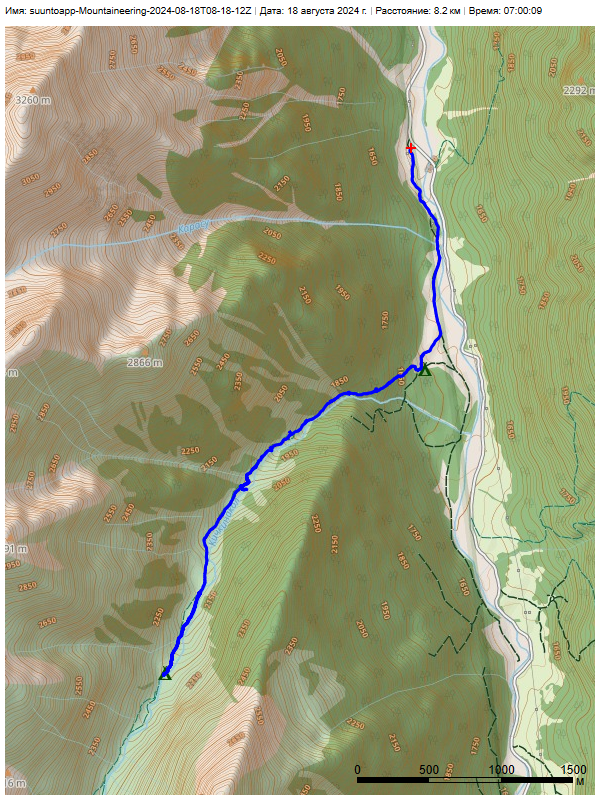
\includegraphics[angle=0, width=0.3\linewidth]{../pics/mini_maps/18}
	\label{fig:mini_18}
\end{figure}


Приезжаем в г. Минеральные Воды в 03:40. Встречаемся на вокзале с участником, прибывшим на день раньше и загружаемся в машину Бориса Саракуева. В 04:00 отправляемся на место старта (мост через р. Учкулан, N 43.38668\degree~E 41.98961\degree), куда прибываем в \alert{СКОЛЬКО?}. Разпределяем заброски, отдаём их водителю и выдвигаемся на маршрут в \alert{СКОЛЬКО?}. Первые 1.5 км до коша проходим по д.р. Учкулан, затем тропа проходит через калитку и поворачивает направо, на подъём в висячую долину р. Кичкинакол Джалпаккольский.

\begin{figure}[h!]
	\centering
	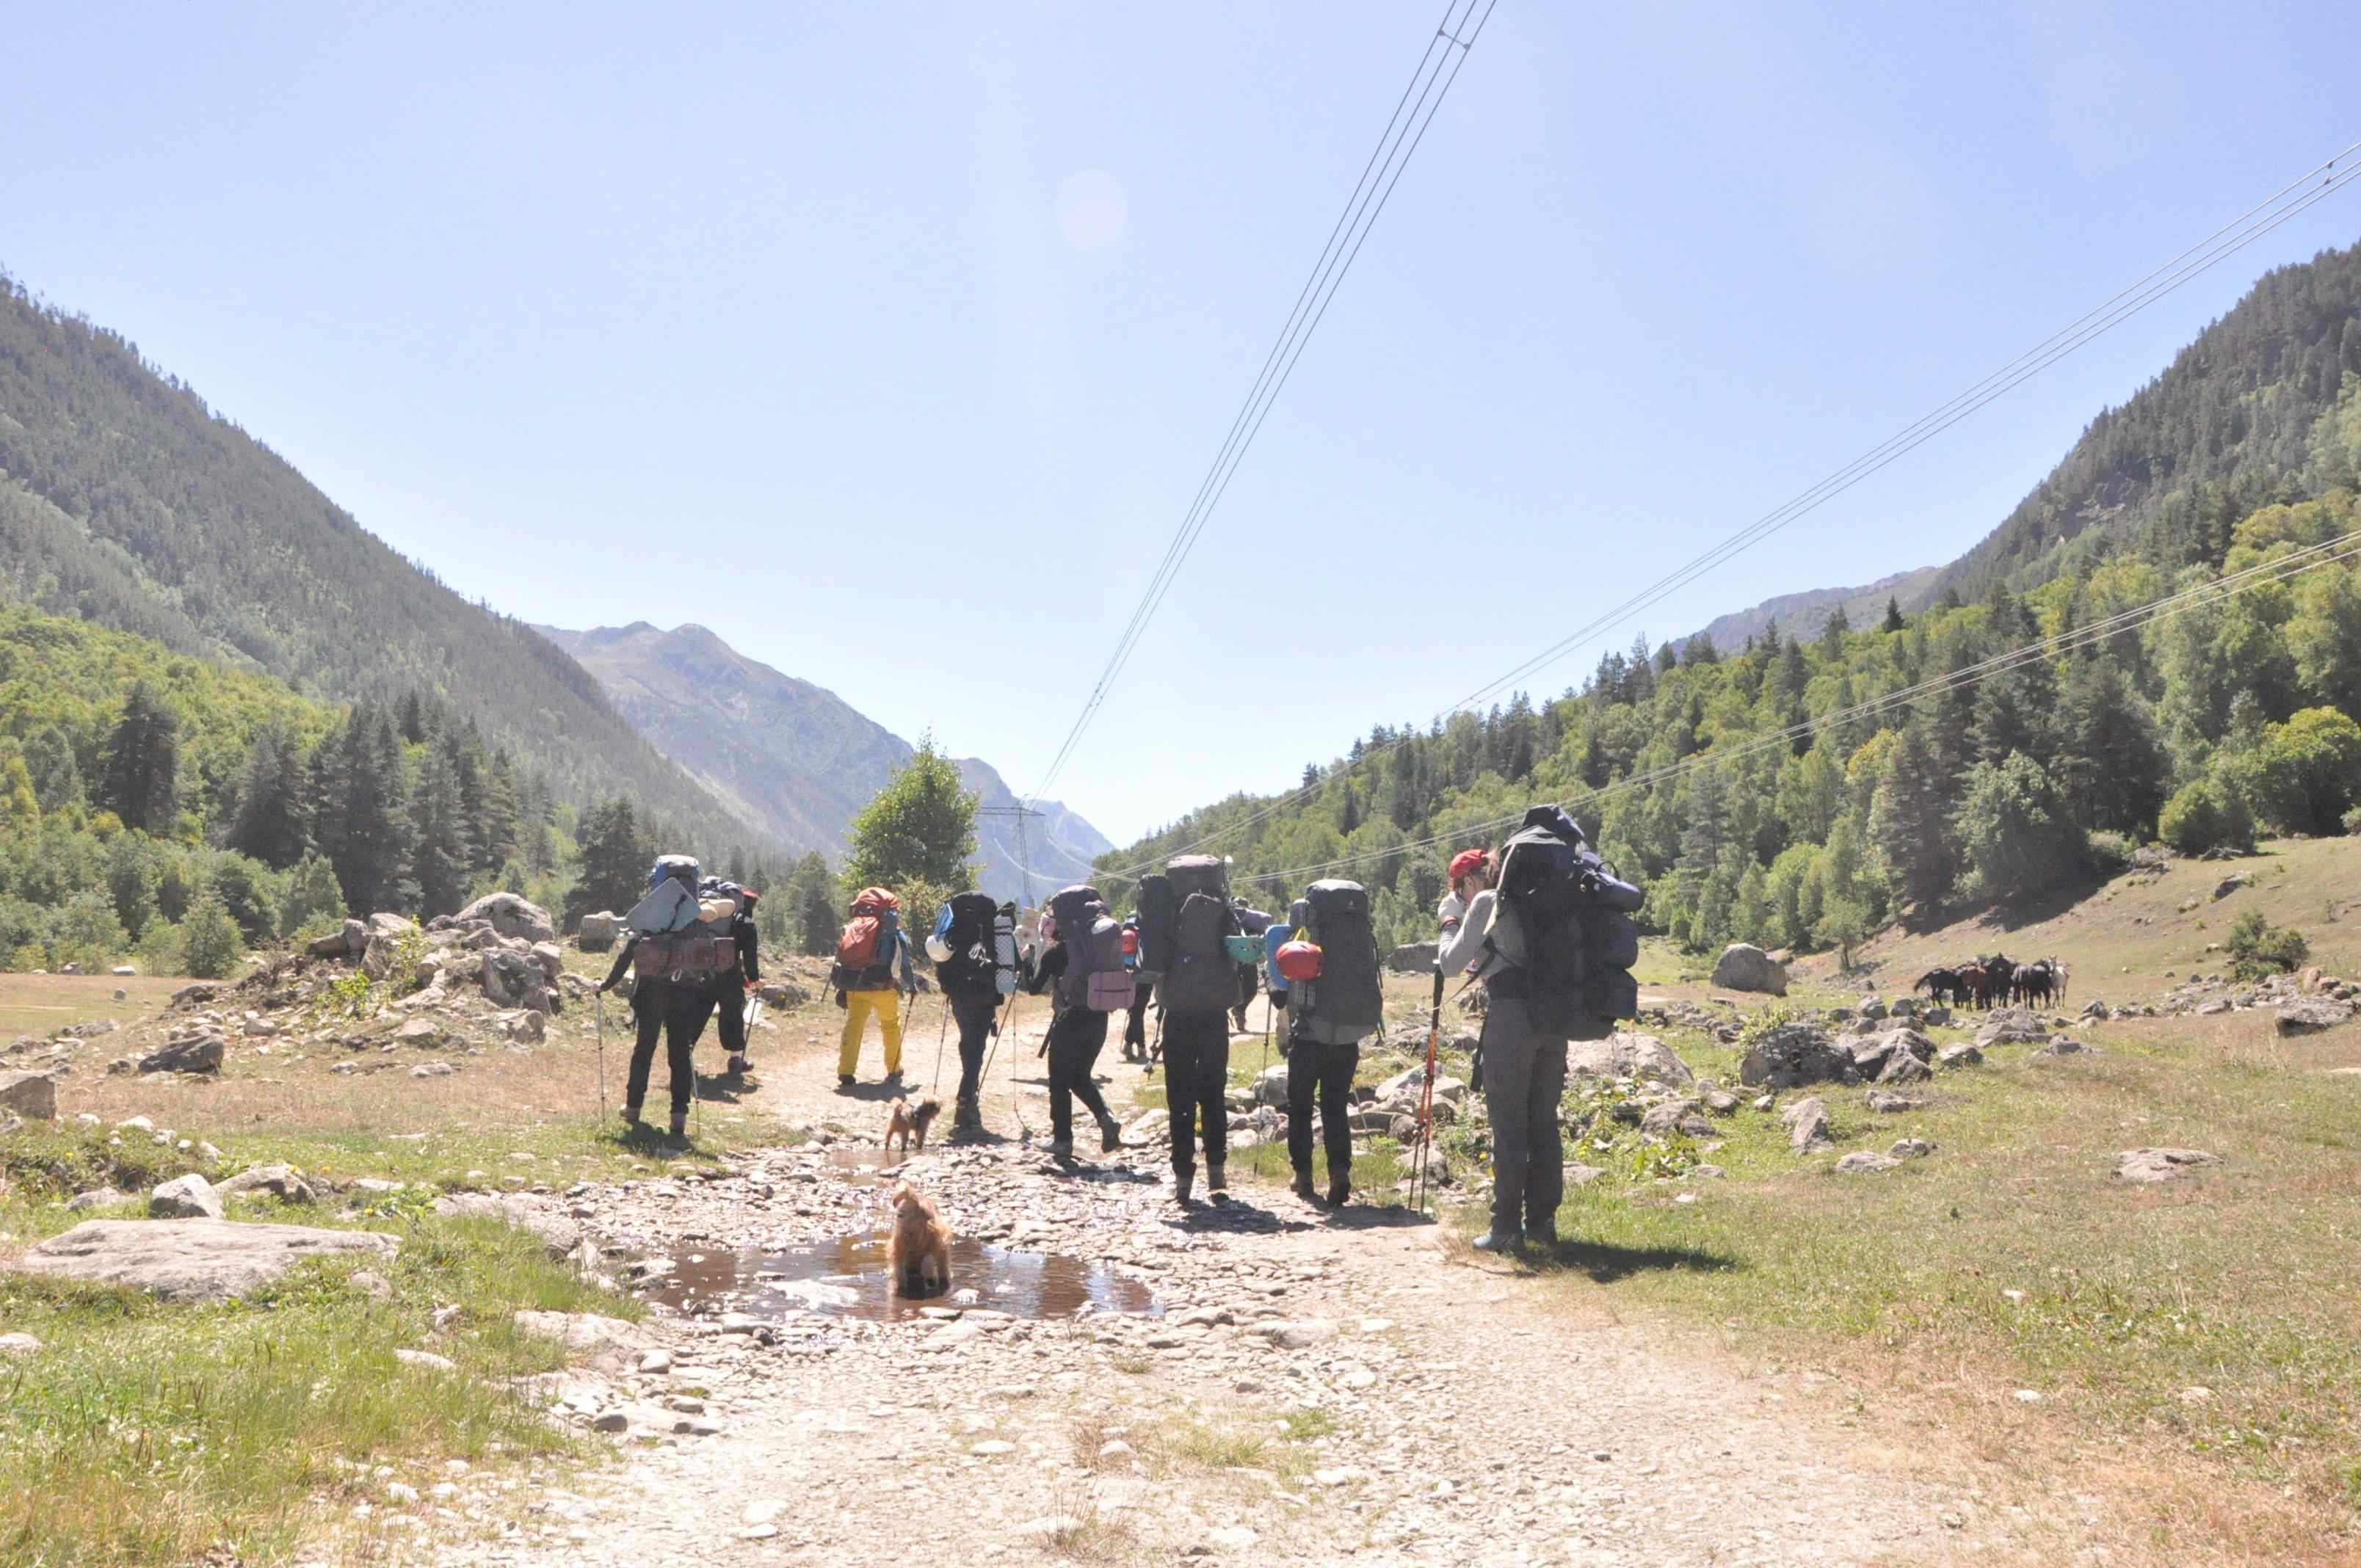
\includegraphics[width=0.7\linewidth]{../pics/DSC_0412}
	\caption{группа на старте маршрута в д.р. Учкулан}
	\label{fig:uchkulan}
\end{figure}


\begin{figure}[h!]
	\centering
	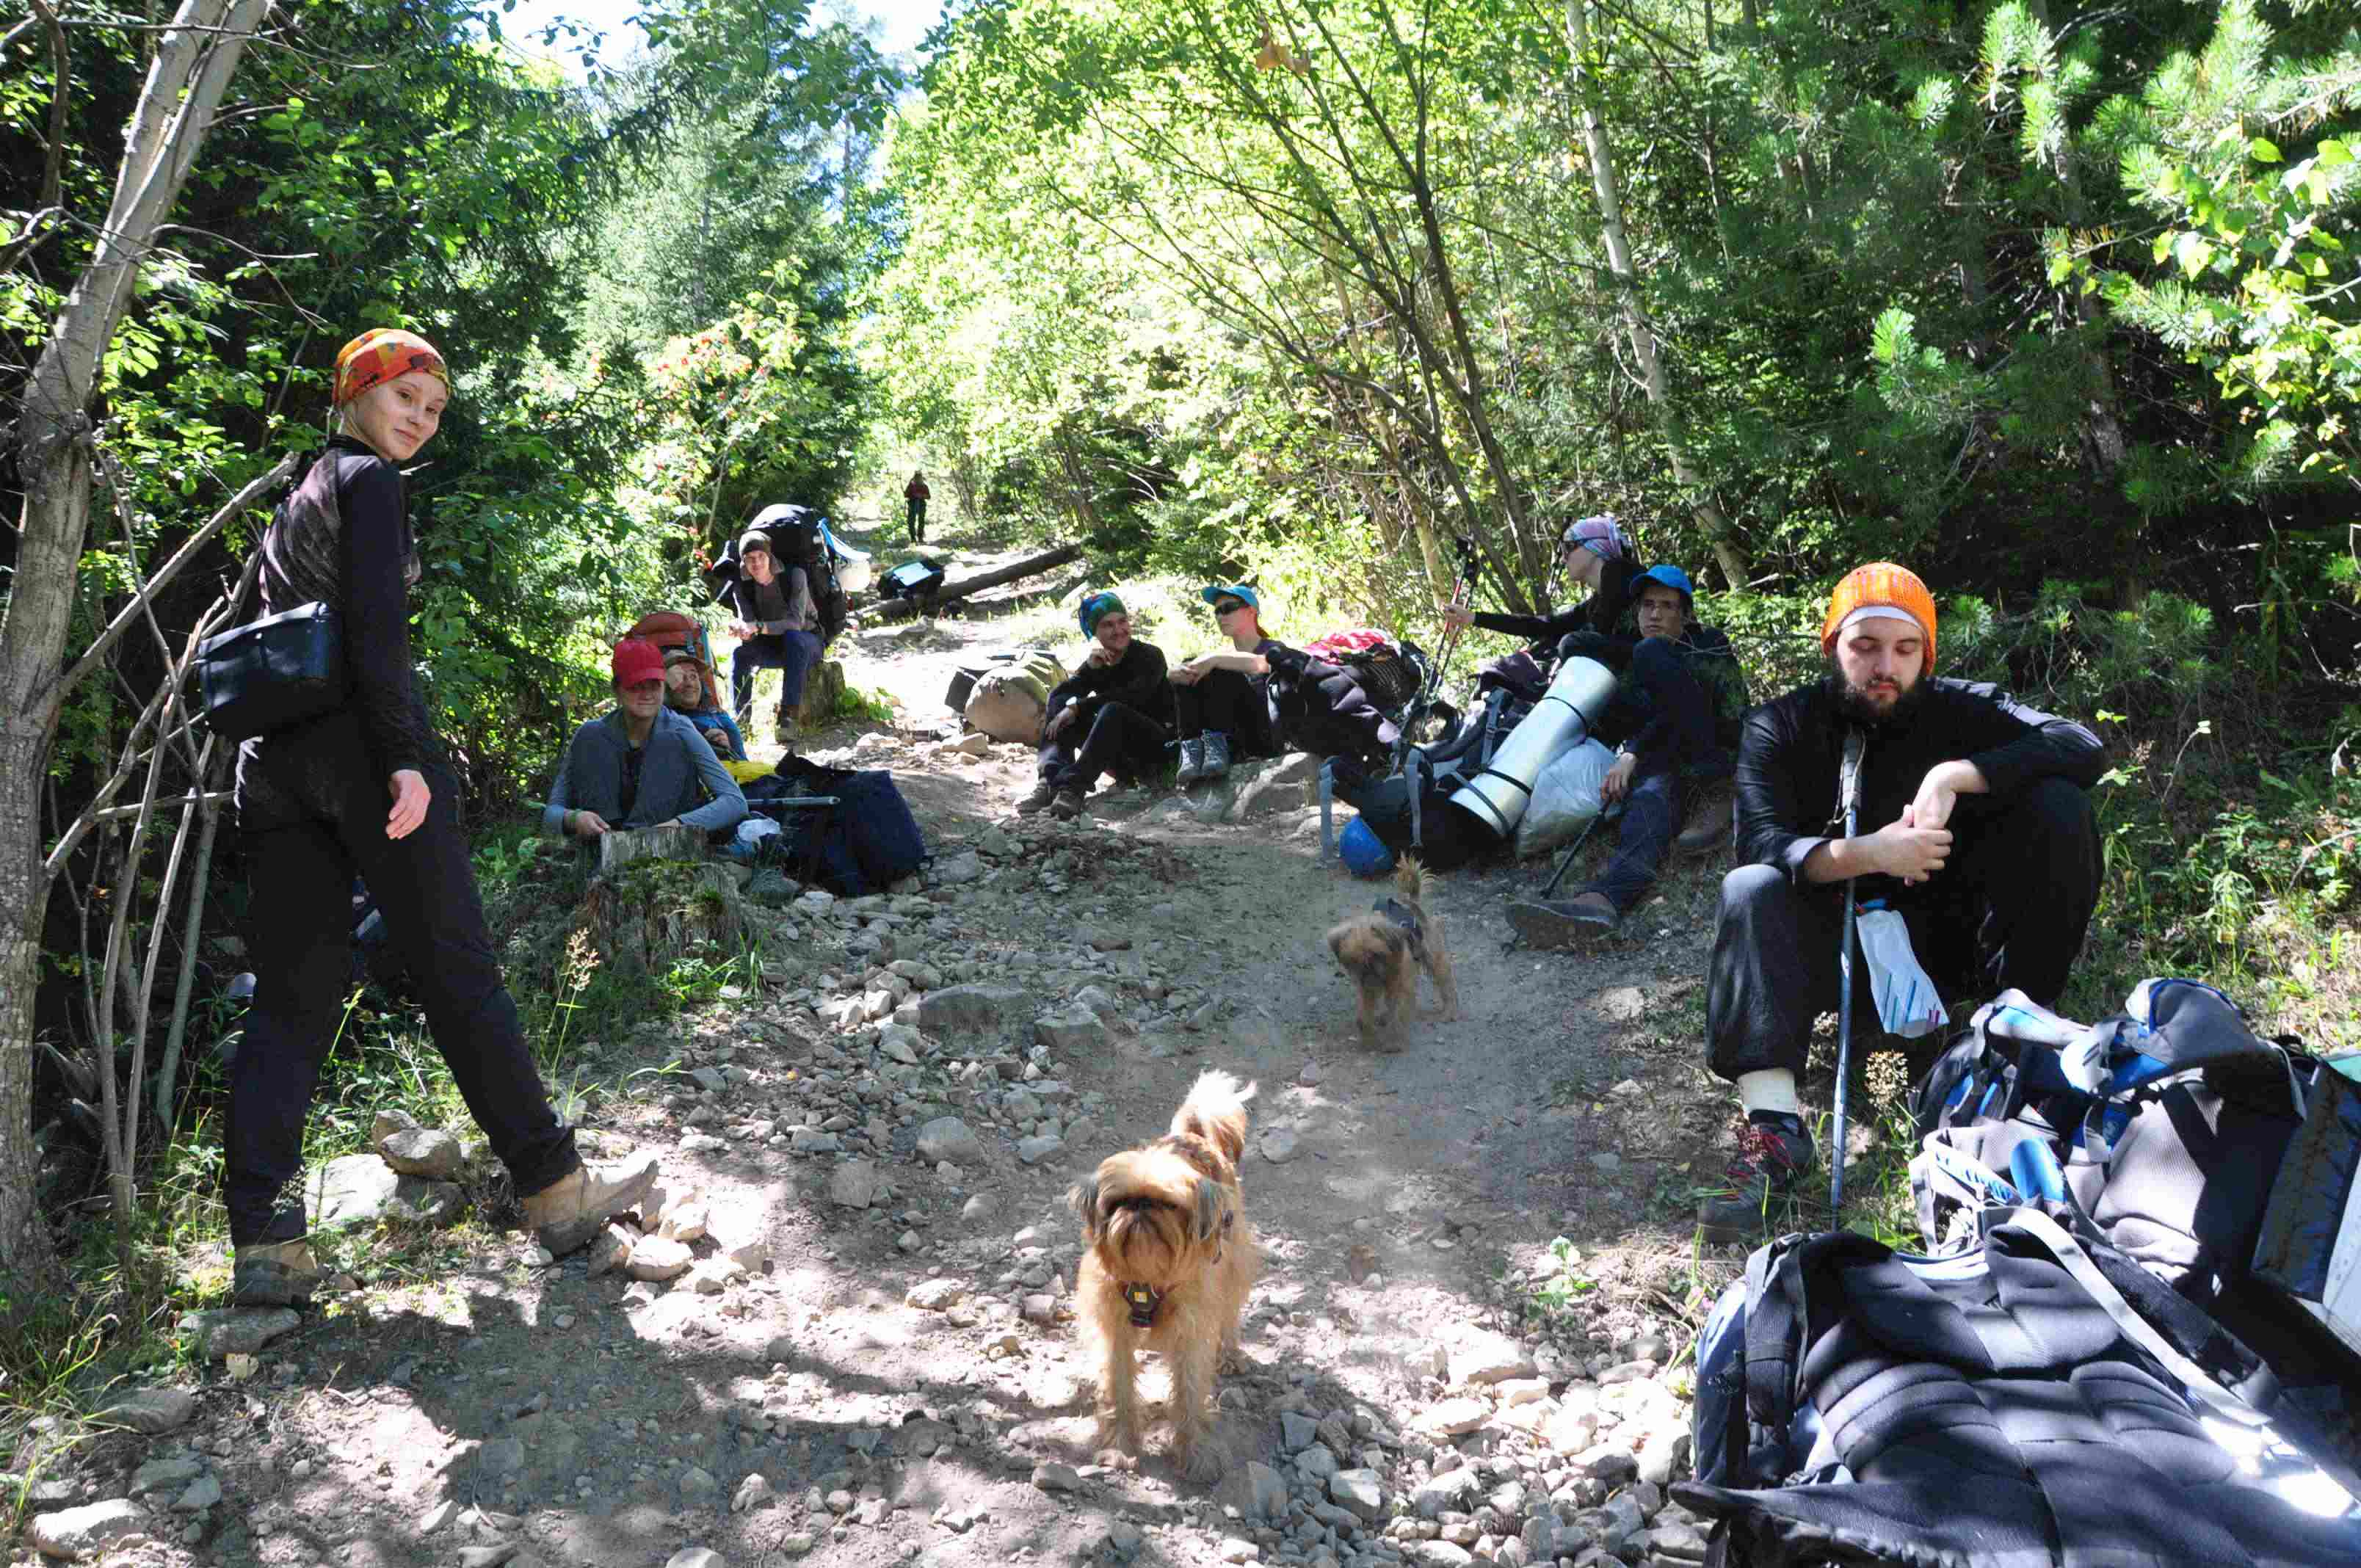
\includegraphics[width=0.7\linewidth]{../pics/DSC_0436}
	\caption{Подъём по тропе в д.р. Кичкинакол Уллукёльский}
	\label{fig:DSC_0436}
\end{figure}

Подъём в висячую долину идёт по хорошей тропе со средний уклоном порядка 20\degree (рис.~\ref{fig:DSC_0436}). Идём не спеша, в режиме 20/5, разгружаем отстающих участников. В \alert{СКОЛЬКО?} заканчиваем подъём в долину и устраиваем обед.

\begin{figure}[h!]
	\centering
	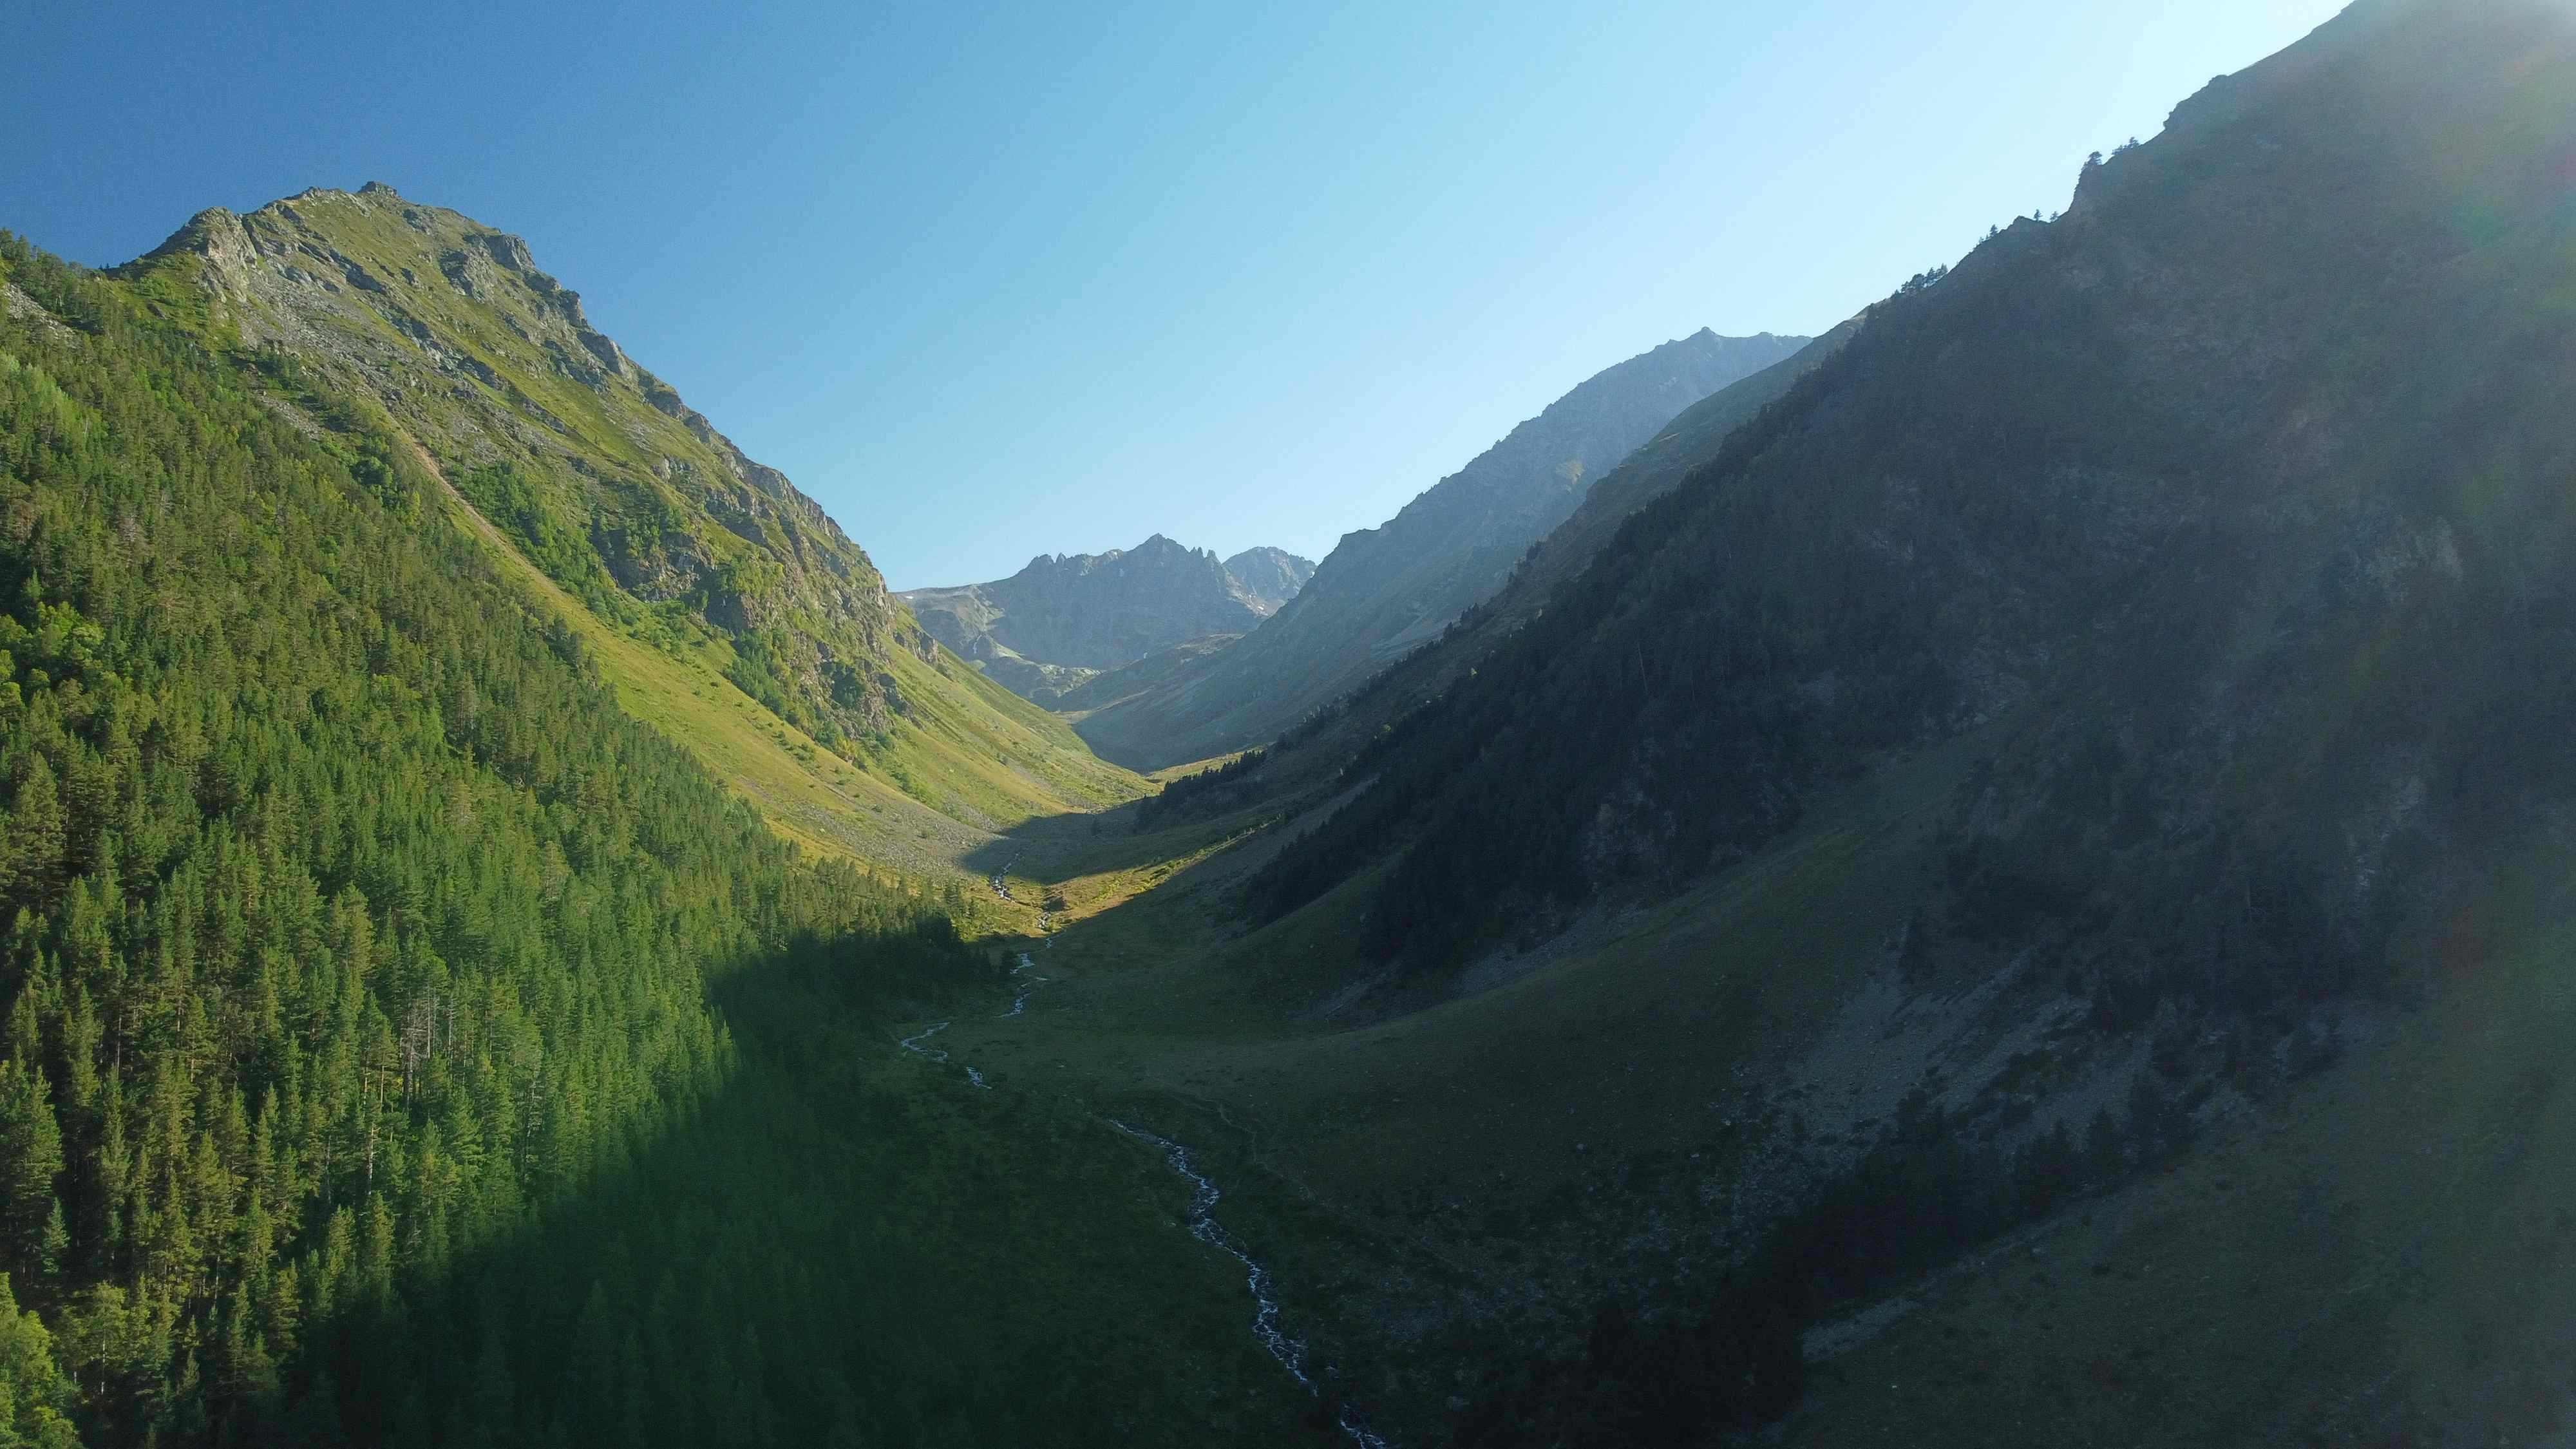
\includegraphics[width=0.7\linewidth]{../pics/DJI_0805}
	\caption{д.р. Кичкинакол Джалпаккольский}
	\label{fig:kichkinakol}
\end{figure}

После обеда в \alert{СКОЛЬКО?} проходим 2 км к оборудованной стоянке возле коша. Рядом местные жители собирают малину. Подумав немного и устроив разведку, поднимаемся ещё немного выше и встаём на место ночёвки на оборудованной стоянке возле дерева на небольшом разливе реки. Координаты м.н. N 43.35392\degree~E 41.96858\degree.
\begin{figure}[h!]
	\centering
	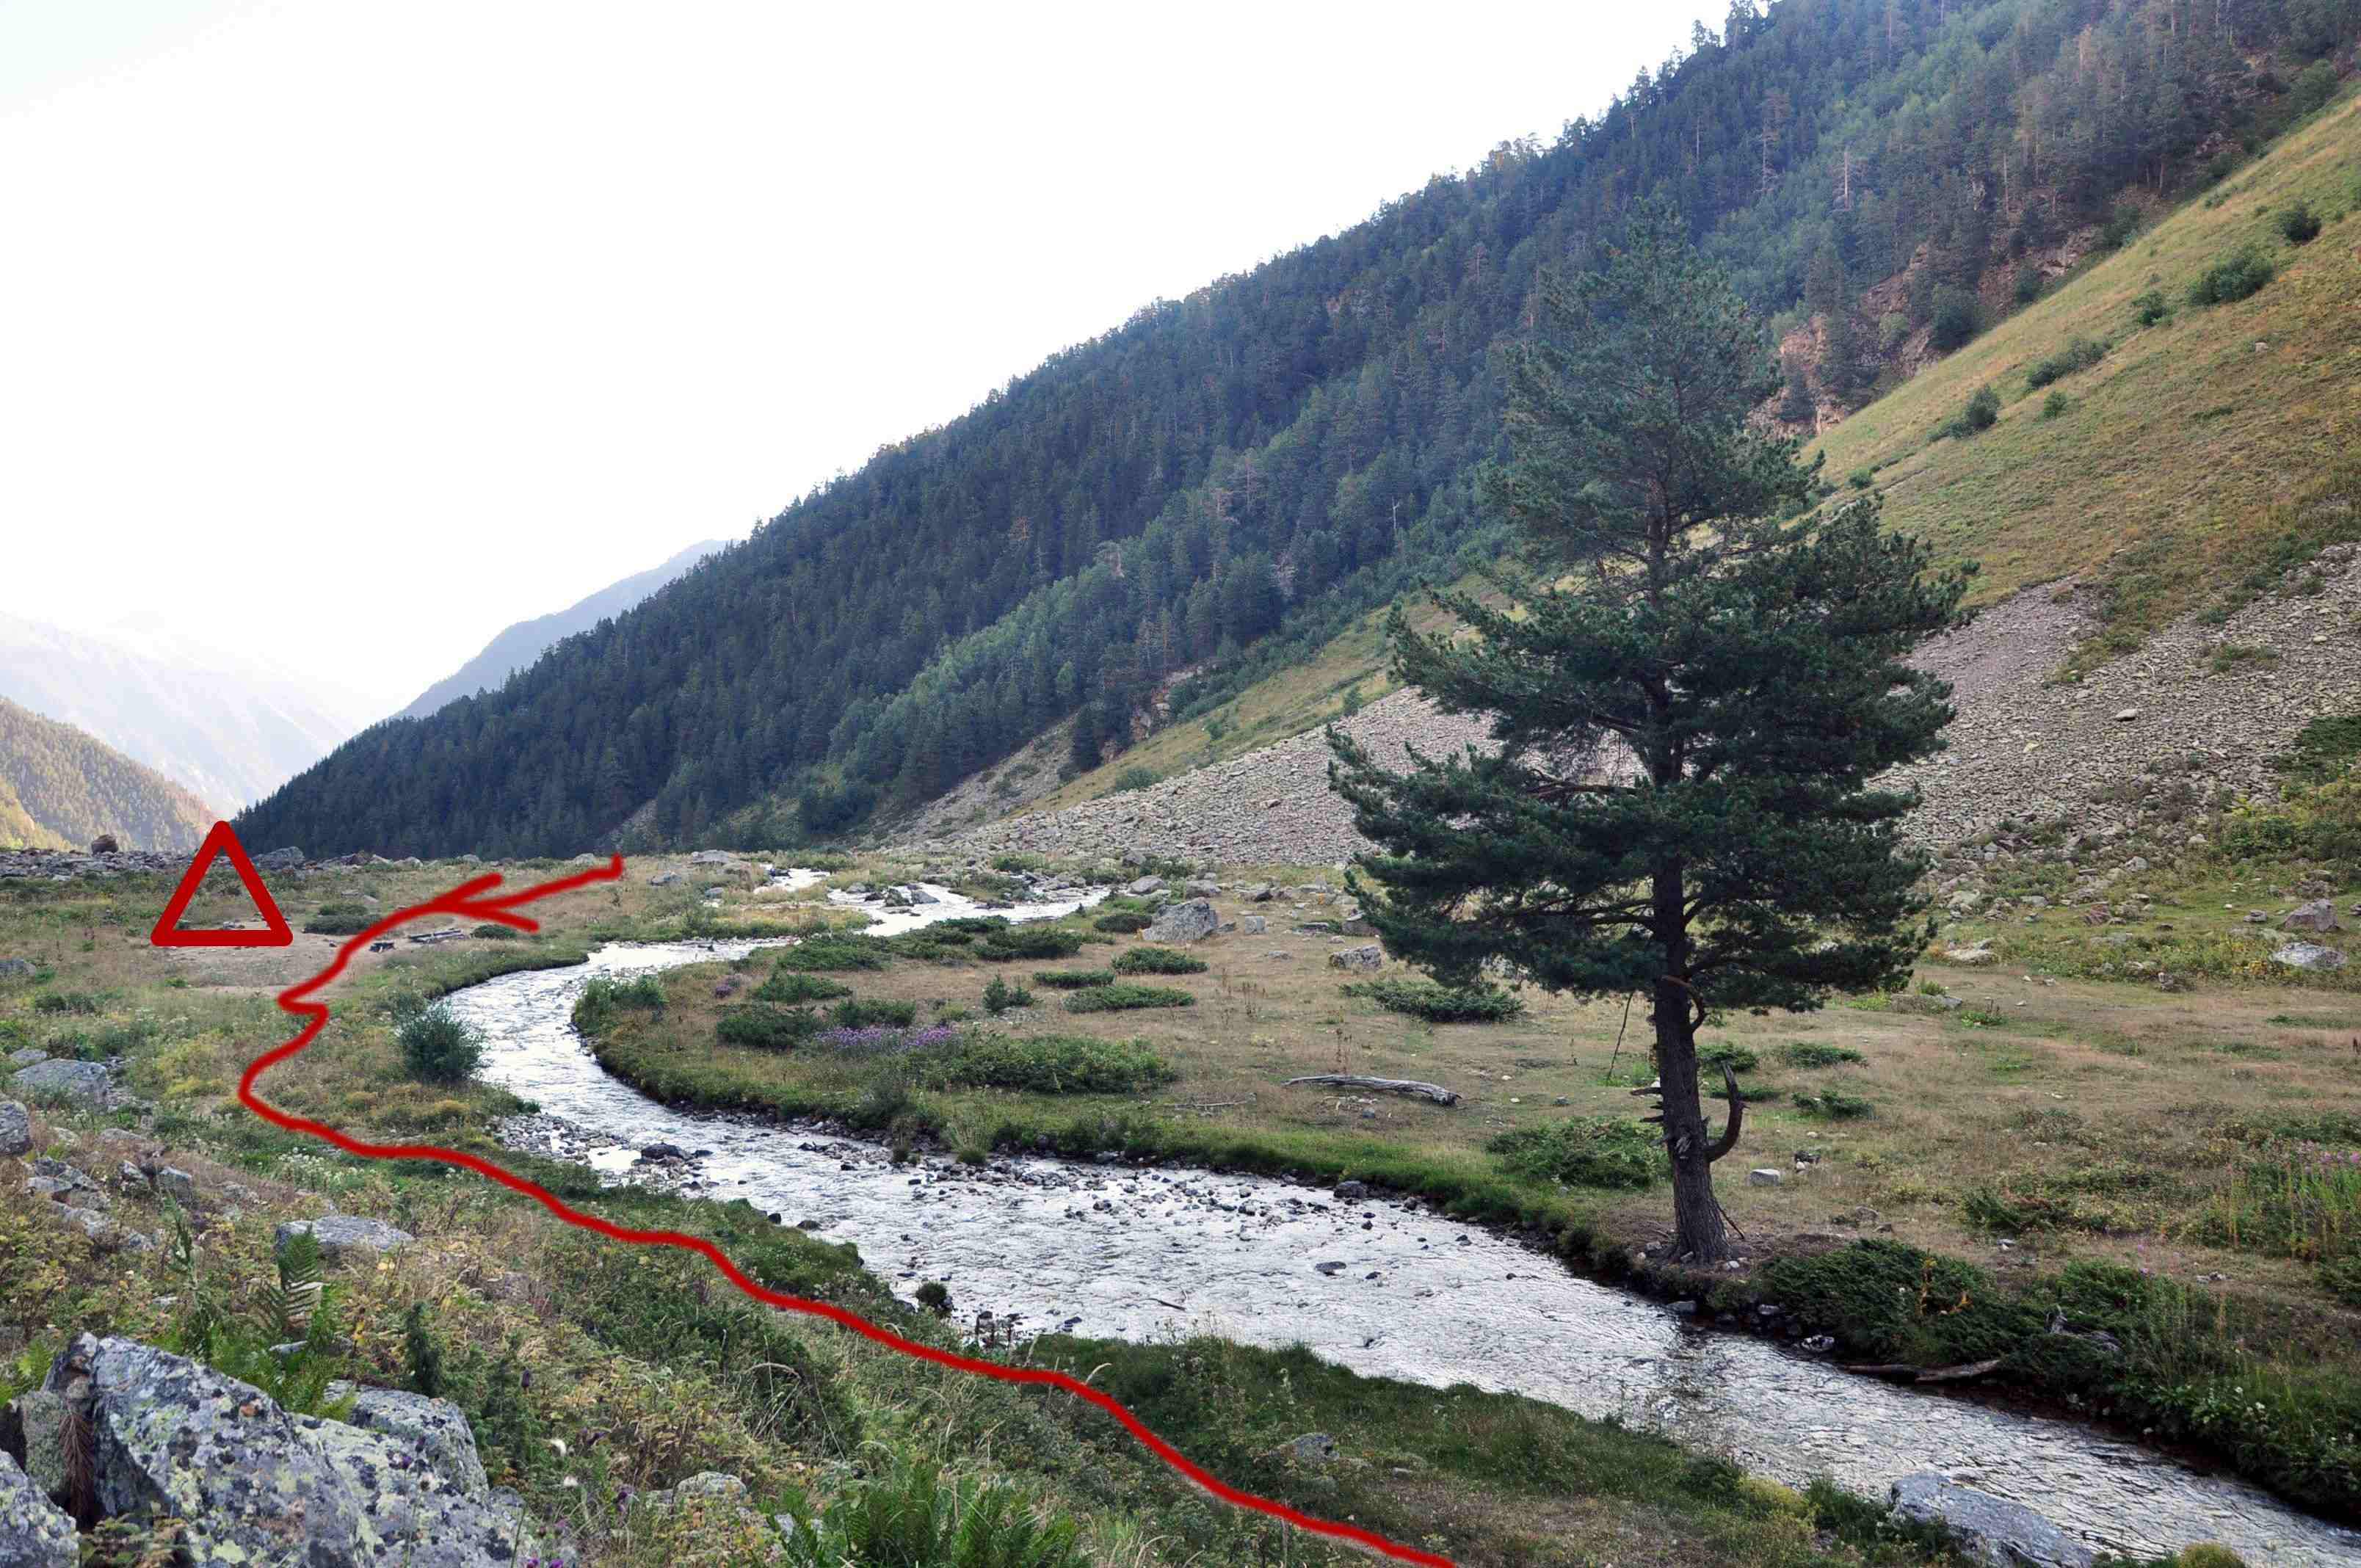
\includegraphics[width=0.7\linewidth]{../pics/camp_18}
	\caption{Место ночёвки 18-19.08}
	\label{fig:camp_18}
\end{figure}


\newpage
\subsection{19 августа. Д.р. Кичкинакол Уллукёльский}
\textit{Метеоусловия: утром, днём, вечером ясно, тепло.}

\begin{figure}[h!]
	\centering
	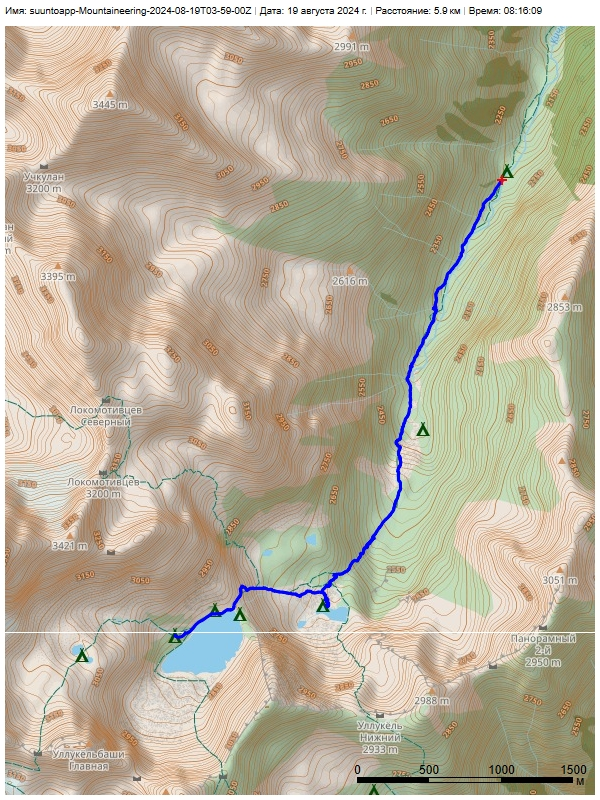
\includegraphics[angle=0, width=0.7\linewidth]{../pics/mini_maps/19}
	\label{fig:mini_19}
\end{figure}

Подъём дежурных в 05:00; общий подъём в 05:30; выход в 07:30.
Продолжили идти по левому берегу р. Кичкинакол Уллукёльский по хорошо набитой тропе, попутно  пересекая старые короткие участки курумника и небольшие притоки реки. В 08:30 вышли на старое моренное плато (рис. \ref{fig:DSC_0692}).

\begin{figure}[h!]
	\centering
	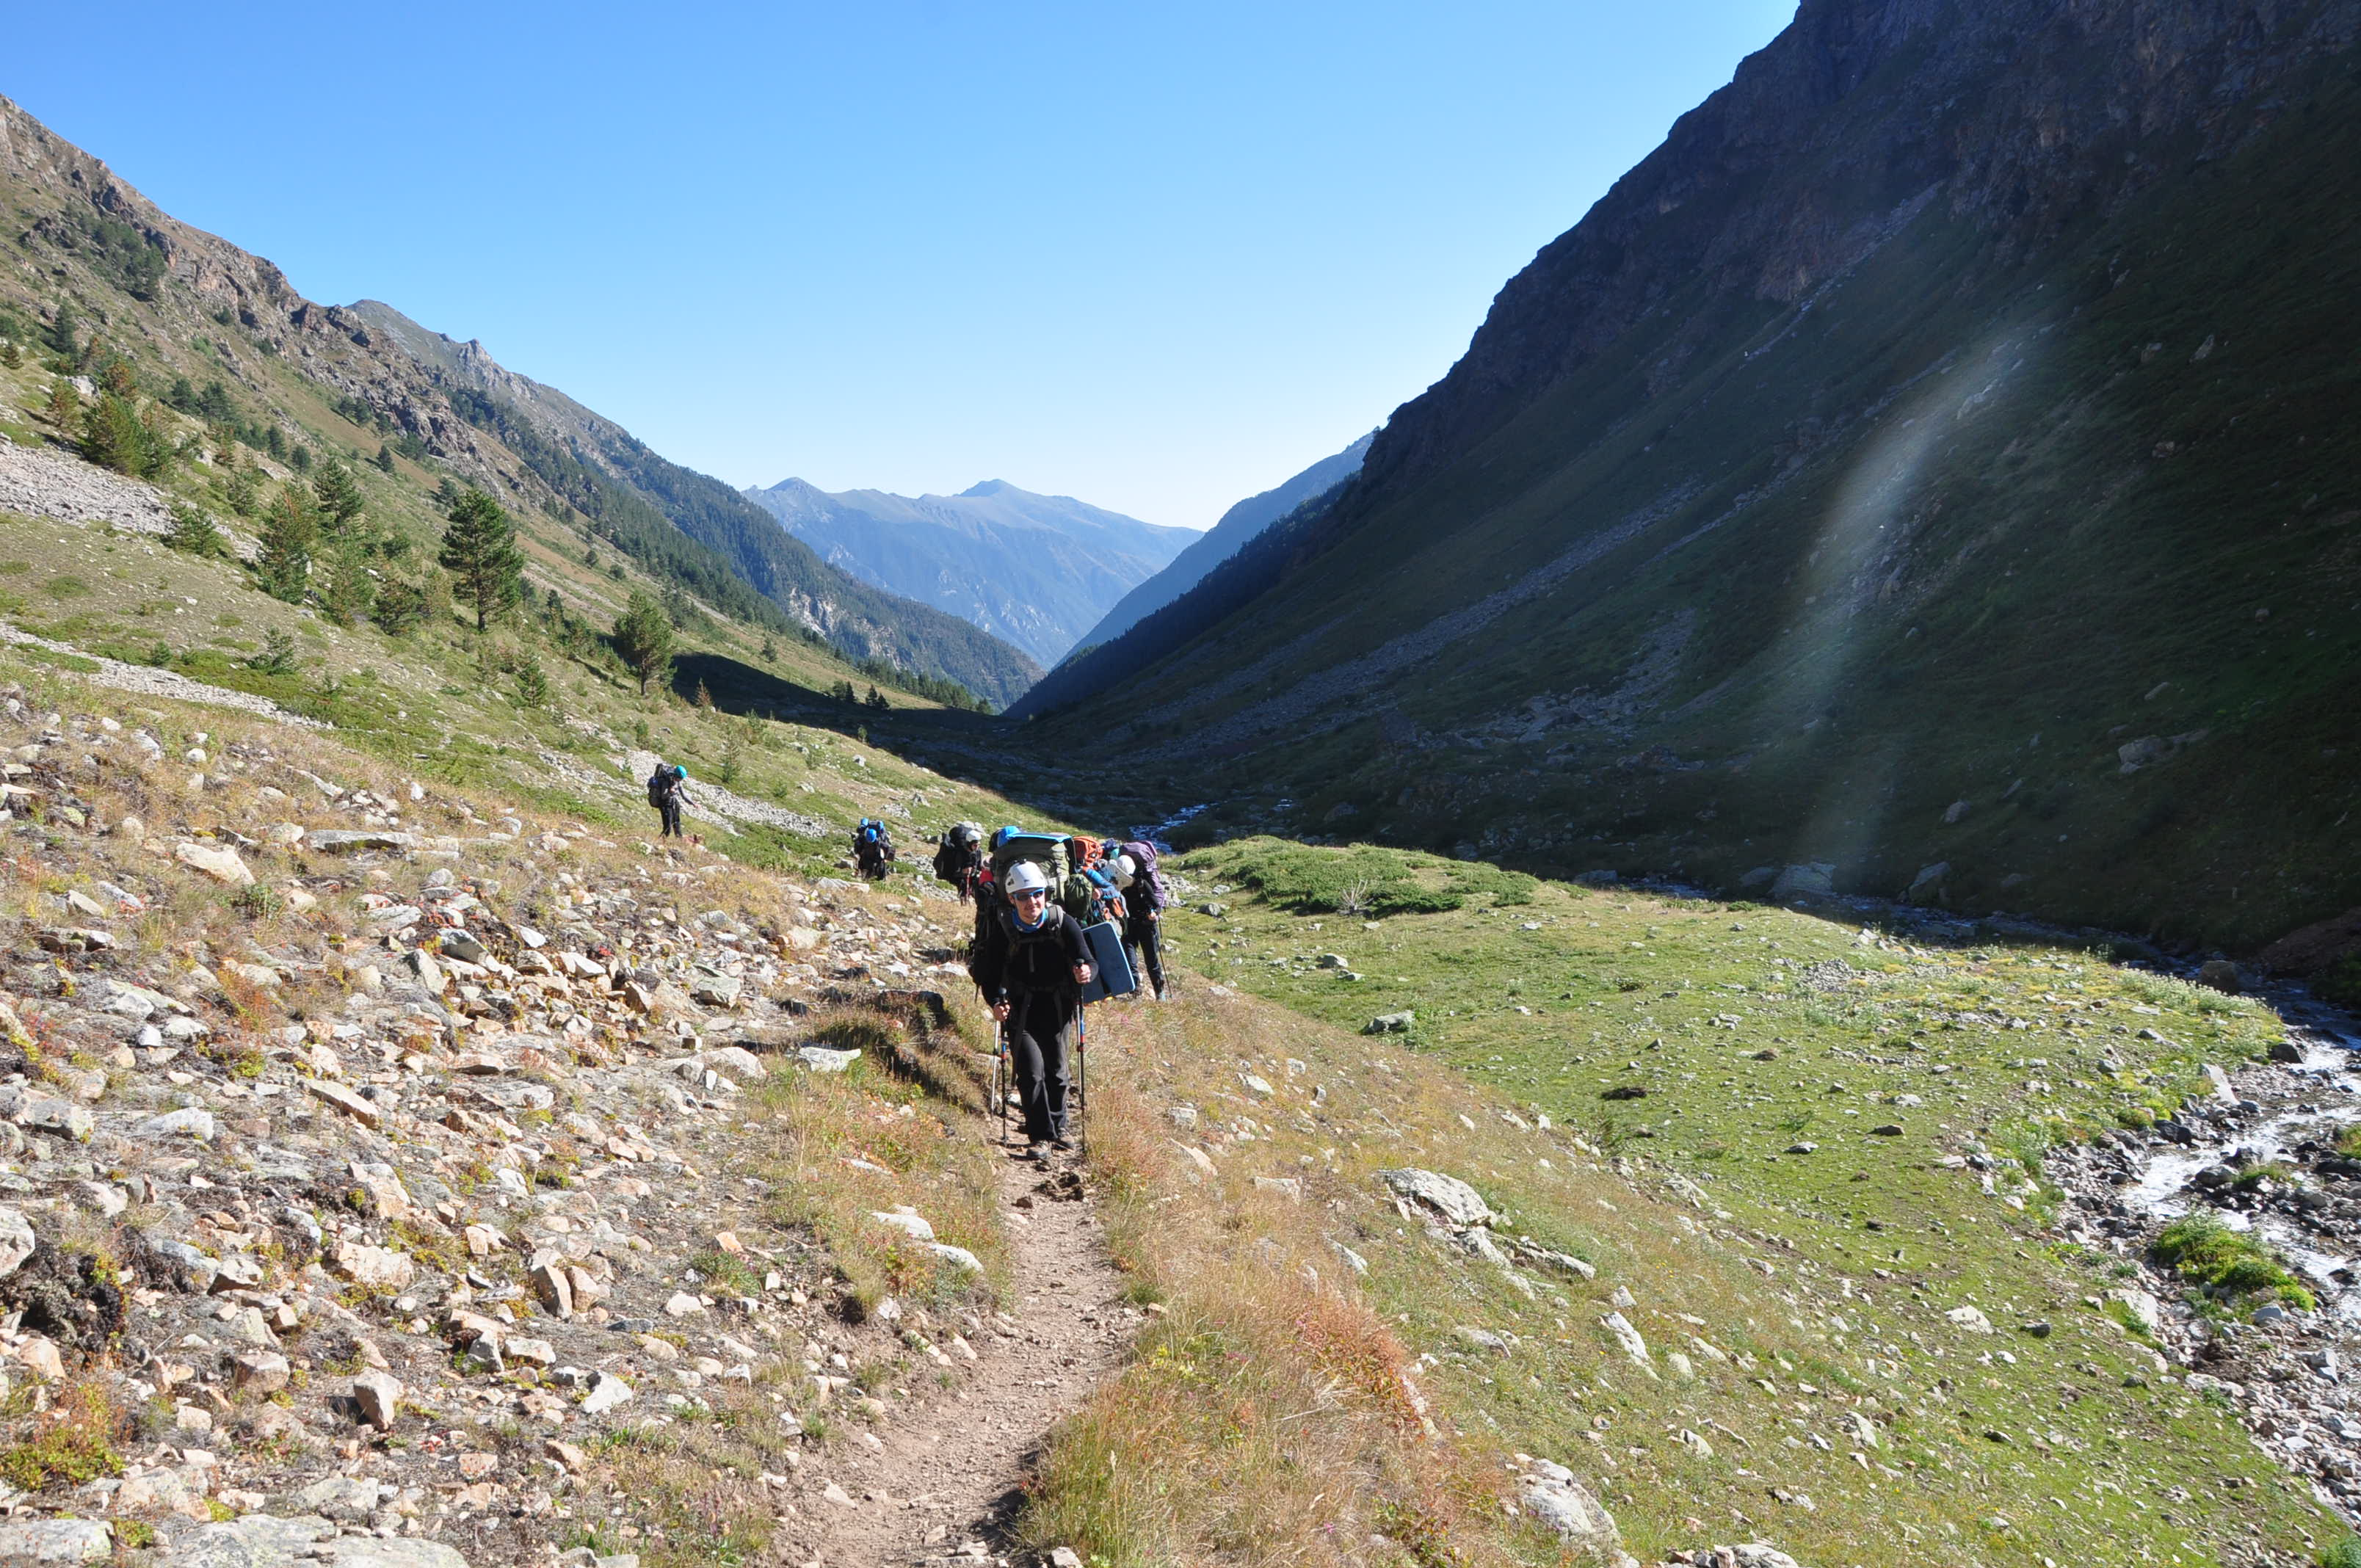
\includegraphics[width=0.7\linewidth]{../pics/DSC_0692}
	\caption{Группа в верховьях д.р. Кичкинакол Уллукёльский}
	\label{fig:DSC_0692}
\end{figure}

Путь от плато к оз. Гитче-Кёль идёт как по левому, так и по правому орогр. берегам р. Кичкинакол Уллукёльский. Мы выбрали первый вариант в силу большей его распространённости и маркированности турами. 

\begin{figure}[h!]
	\centering
	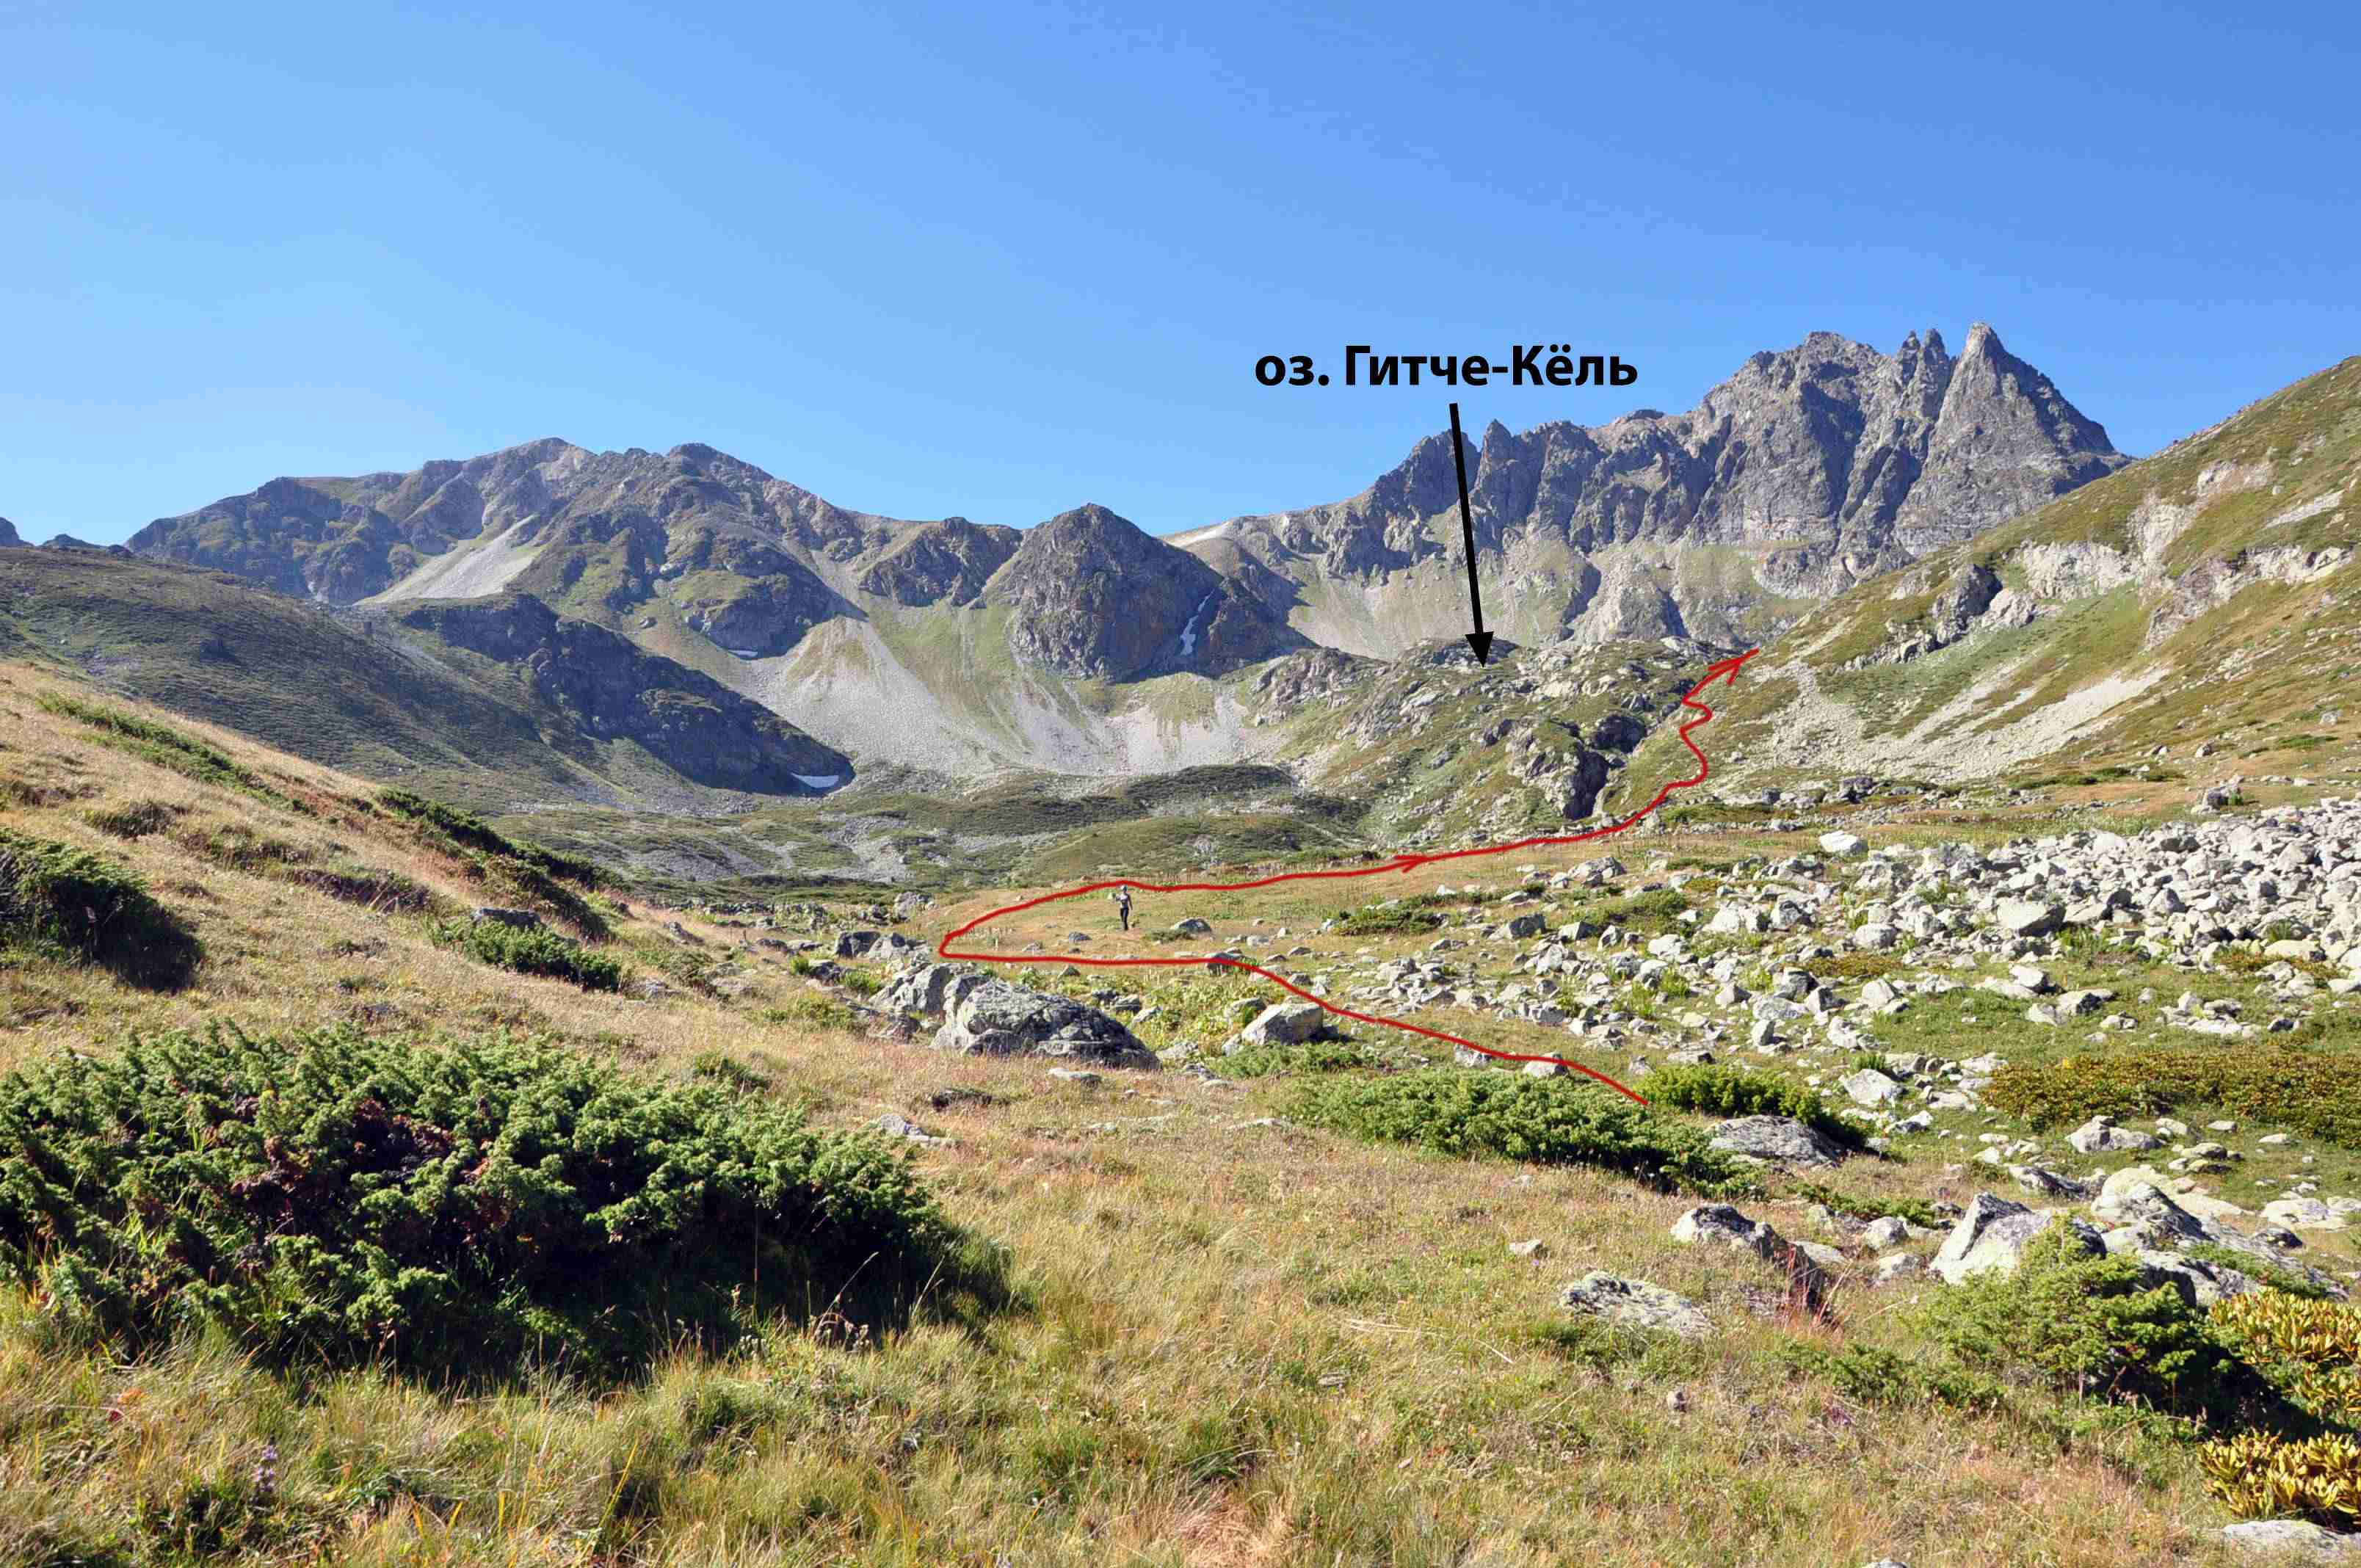
\includegraphics[width=0.7\linewidth]{../pics/DSC_0718}
	\caption{Путь подъёма к оз. Гитче-Кёль}
	\label{fig:DSC_0718}
\end{figure}

Преодолев моренную дамбу крутизной до 25\degree и высотой до 90 м, в 11:15\textcolor{teal}{(или в 10:47?)} вышли к оз. Гитче-Кёль (ЧХВ=\alert{СКОЛЬКО?}) и встали на обед. 
Погода стояла жаркая, мы не спеша приго обед, купаемся и окончательно решили идти по основному маршруту на пер. Уллу-Кёль Восточный, а не на пер. Уллу-Кёль Нижний.



\begin{figure}[h!]
	\centering
	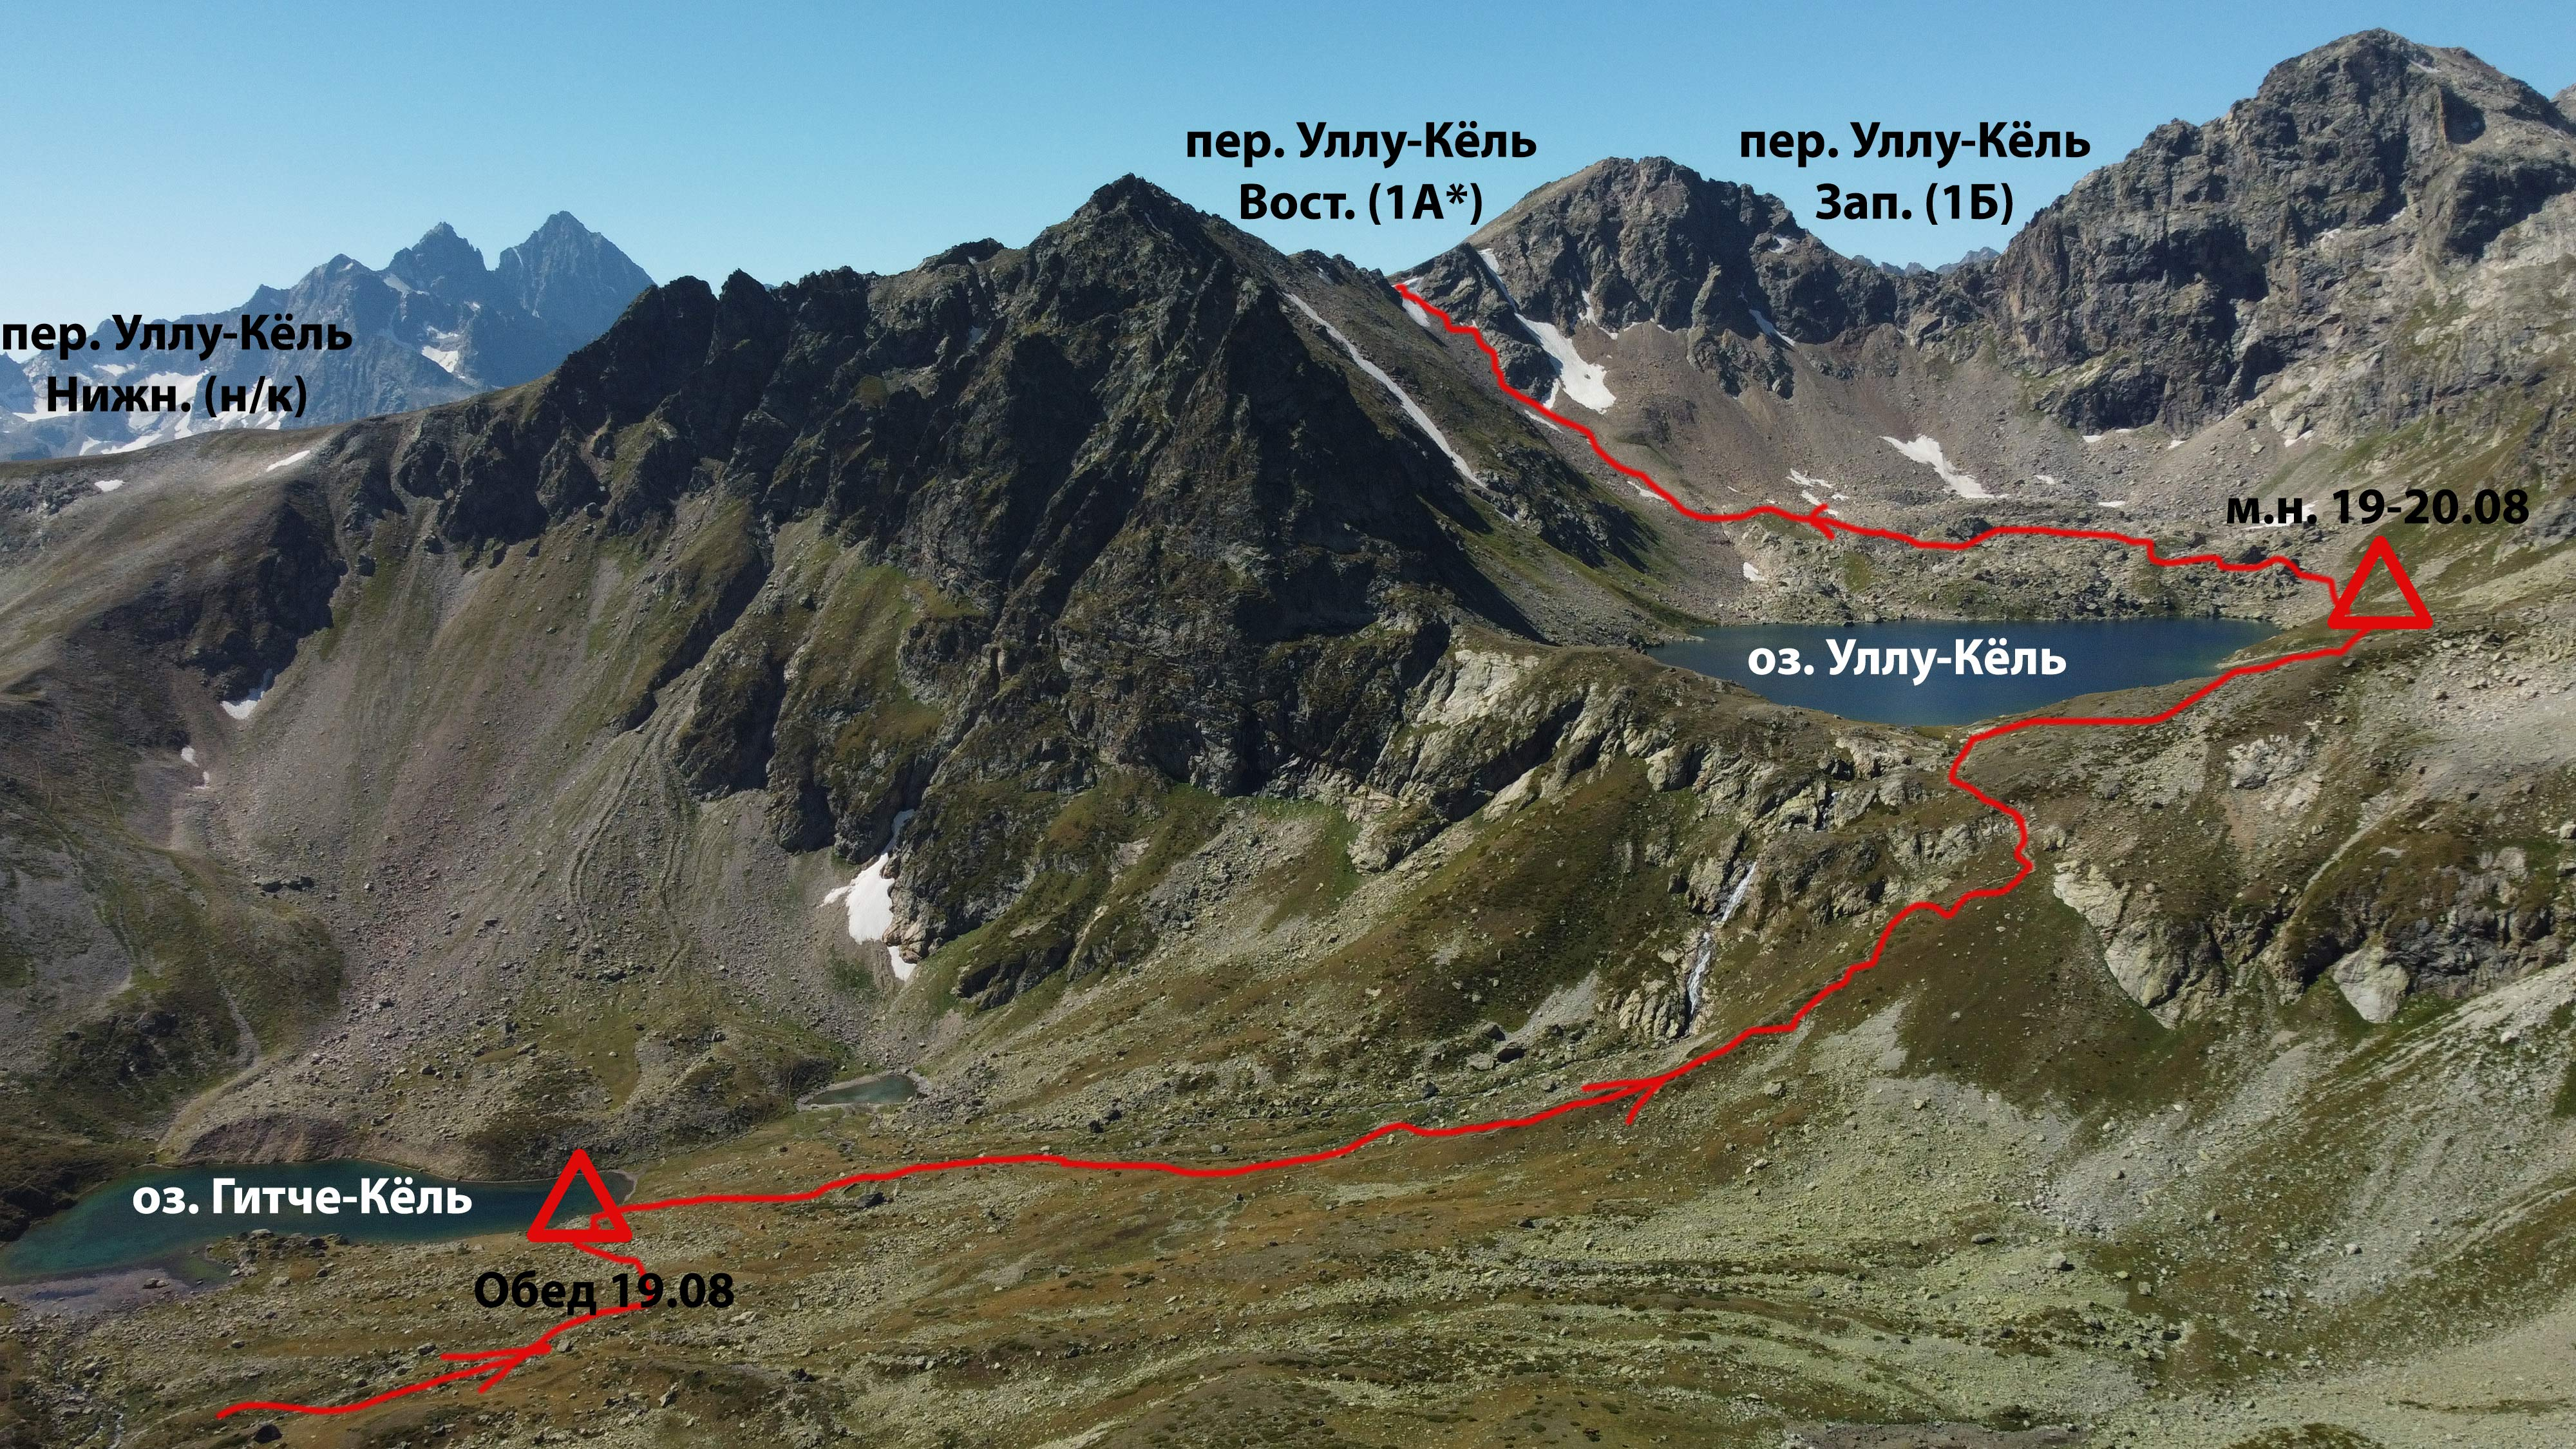
\includegraphics[width=0.7\linewidth]{../pics/ullu_kuel_route}
	\caption{Дорога до озёр и далее на перевал}
	\label{fig:ullu_kuel_route}
\end{figure}

\begin{figure}[h!]
	\centering
	\begin{turn}{0}
		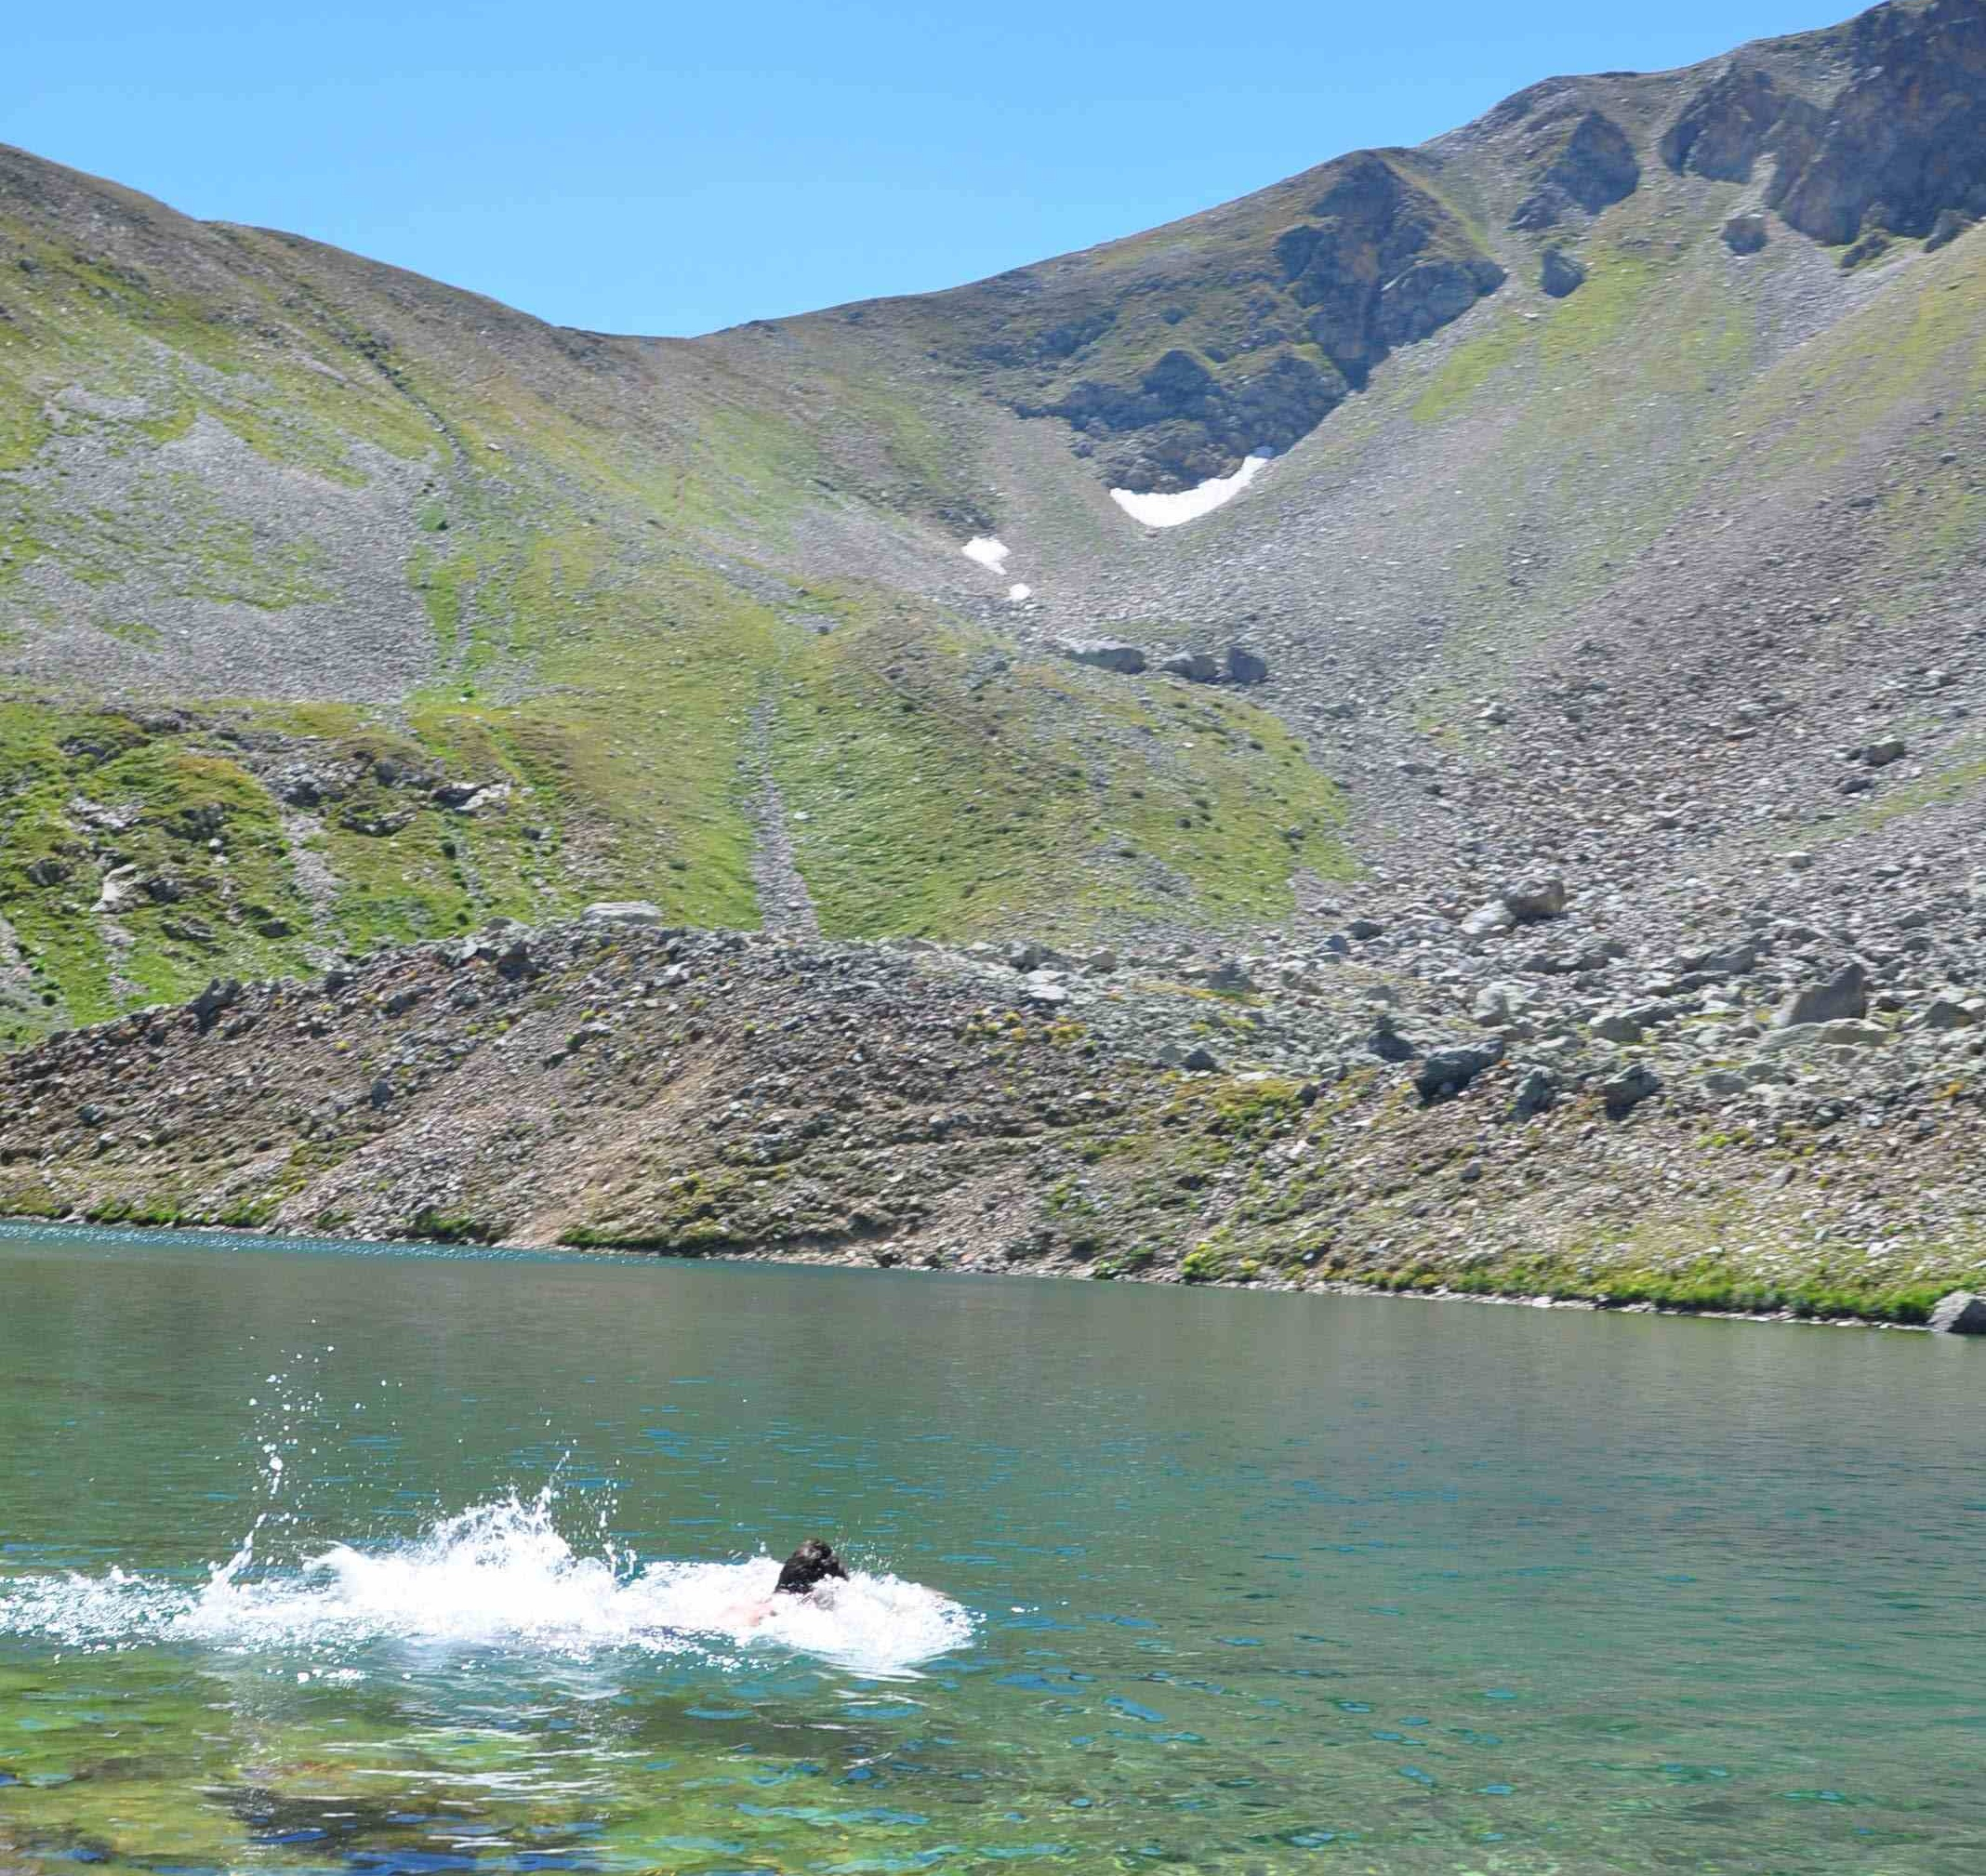
\includegraphics[width=0.7\linewidth]{../pics/DSC_0774}
	\end{turn}
	\caption{Купаемся в оз. Гитче-Кёль}
	\label{fig:DSC_0774}
\end{figure}

К 15:00 вышли на северо-восточную оконечность озера, и в 15:15 становимся на ночёвку на оборудованной стоянке, координаты м.н. N 43.32501\degree E 41.94003\degree

\begin{figure}[h!]
	\centering
	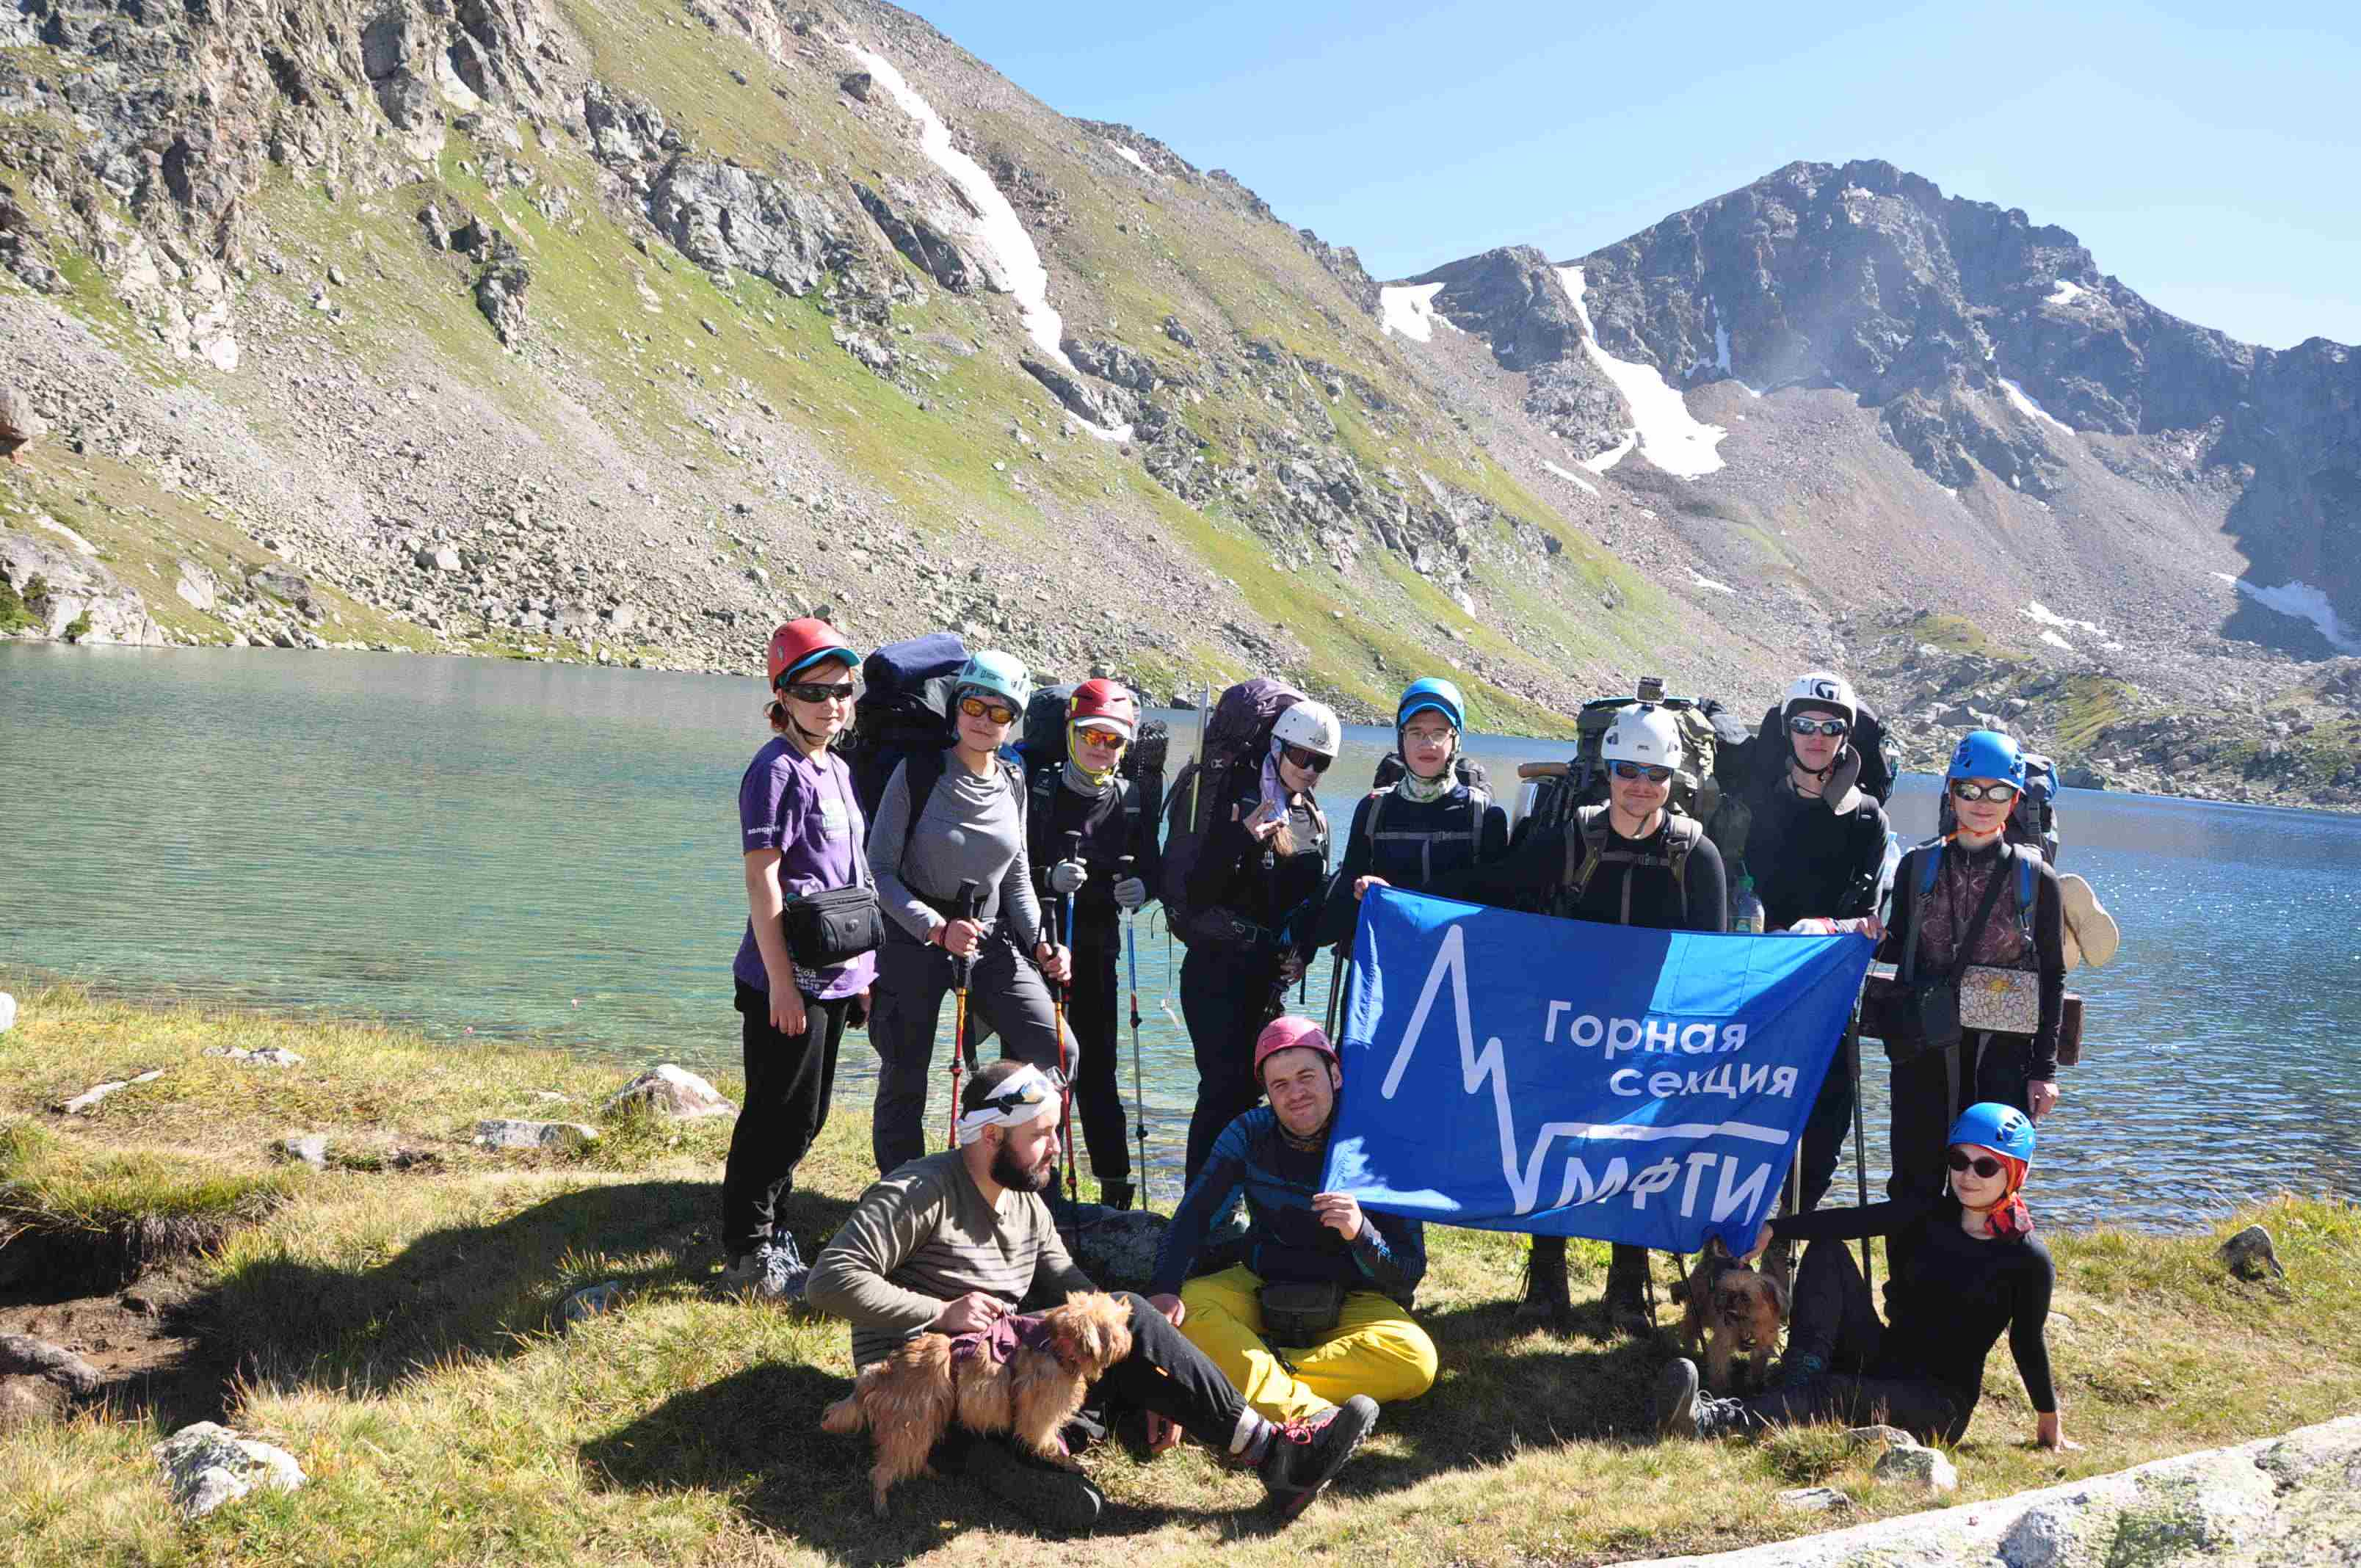
\includegraphics[width=0.7\linewidth]{../pics/DSC_0800}
	\caption{Группа на оз. Уллу-Кёль}
	\label{fig:DSC_0800}
\end{figure}


По случаю полуднёвки решили провести тренировку по хождению в кошках и самозарубанию на снежном склоне, и в 16:10 вышли из лагеря налегке, треверсируя склон выше крупной осыпи, в направлении снежника под пер. Дырявый (1Б). Траверсируемый склон сначала осыпной, далее травянисто-осыпной крутизной до 25\degree. Такая форма рельефа была участникам в новинку, и, как следствие, продвигались мы медленно. Оценив время на тренировку и возвращение, решили дойти до более близкого пологого снежника, отказаться от тренировки самозарубания и только походить в кошках. Сама тренировка заняла около 30 минут. В некоторый момент мимо нас проходит целое семейство горных козлов в количестве 6 штук.
На обратном пути от снежника спускались напрямую к озеру, и затем прошли вдоль его кромки, попутно разведывая завтрашний путь к перевалу. 

Самое проблемное место представляло из себя завалы больших камней на берегу озера. Согласно отчётам \textcolor{teal}{(каким?)}, есть три варианта прохождения этого участка: если ориентироваться по двум\textcolor{teal}{(?)} валунам, то можно пройти прямо под ними, поверху них --- или заранее, сразу как при выходе из лагеря начинаются камни, забирать выше и сразу выходить на моренные гребни над озером. По результатам разведки решено было отдать предпочтение первому варианту.

В лагерь вернулись в 17:50, перед сном устроили фотосессию по случаю красивого звёздного неба и яркой луны (рис. \ref{fig:IMG_20240829_194851}).

\begin{figure}[h!]
	\centering
	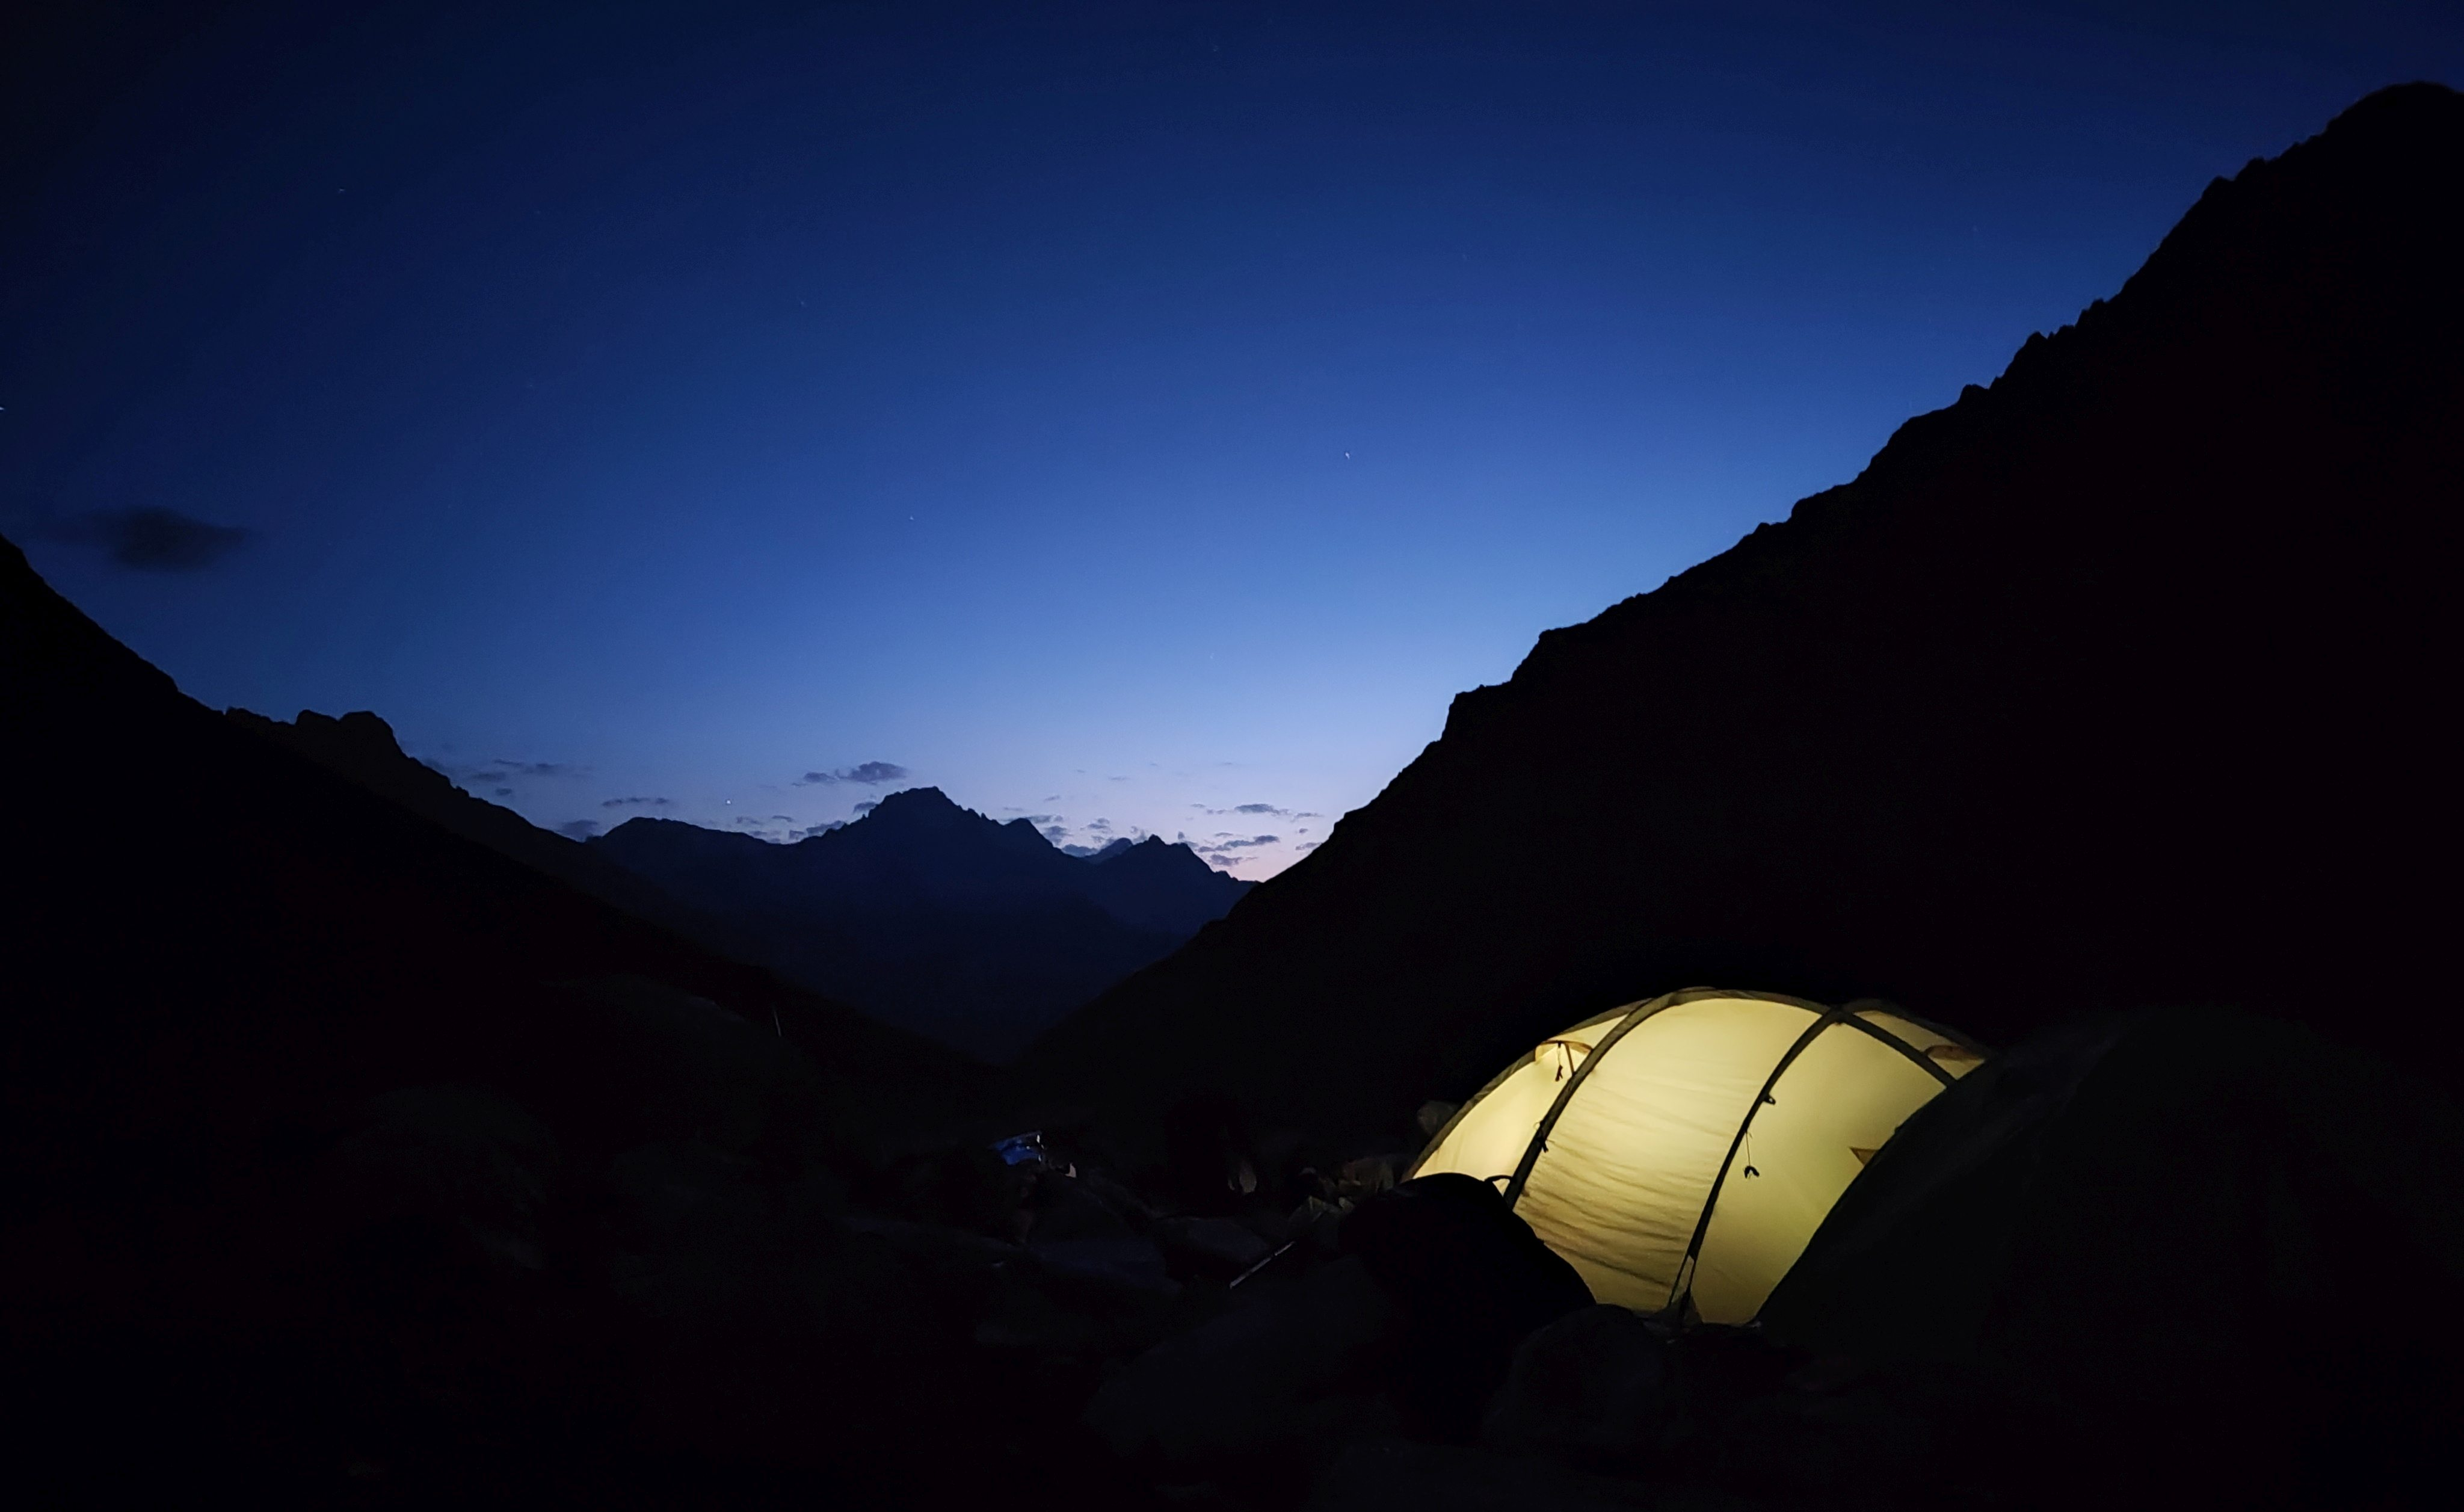
\includegraphics[width=0.7\linewidth]{../pics/IMG_20240829_194851}
	\caption{Место ночёвки 19-20.08}
	\label{fig:IMG_20240829_194851}
\end{figure}

\clearpage
\subsection{20 августа. пер. Уллукёль Восточный (1А*)}
\textit{Метеоусловия: утром, днём ясно, вечером~--- переменная облачность, тепло.}

\begin{figure}[h!]
	\centering
	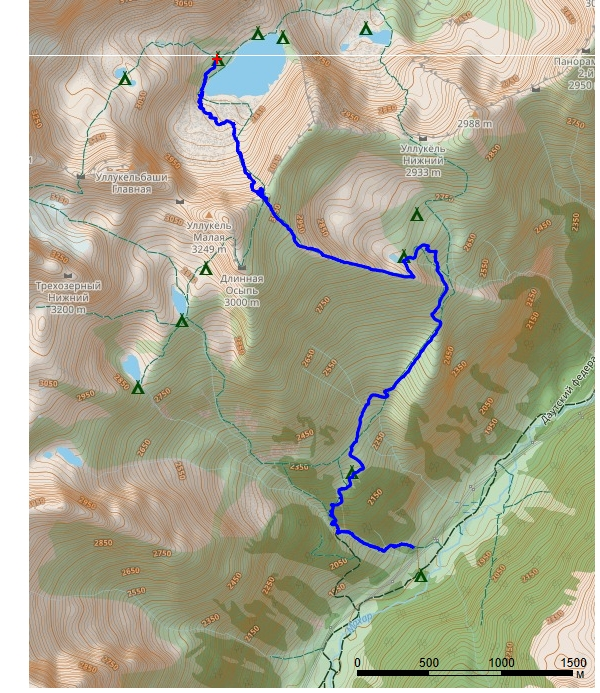
\includegraphics[angle=0, width=0.3\linewidth]{../pics/mini_maps/20}
	\label{fig:mini_20}
\end{figure}

Подъём дежурных в 04:30, общий подъём в 05:00. Выход группы в 07:30. Движемся по разведанному вчера маршруту по крупной осыпи в обход южной оконечности озера. На одном из привалов участнице (Наташе Мироновой) становится нехорошо, и часть пути (ок. 15 мин. ЧХВ) она проходит без рюкзака. Пока доносим рюкзак, группа фотографируется на фоне озера (рис.~\ref{fig:DSC_0907}).

Далее движемся по моренному гребешку и выходим на среднюю осыпь перевального взлёта, прижимаясь к правому пхд борту кулуара..

\begin{figure}[h!]
	\centering
	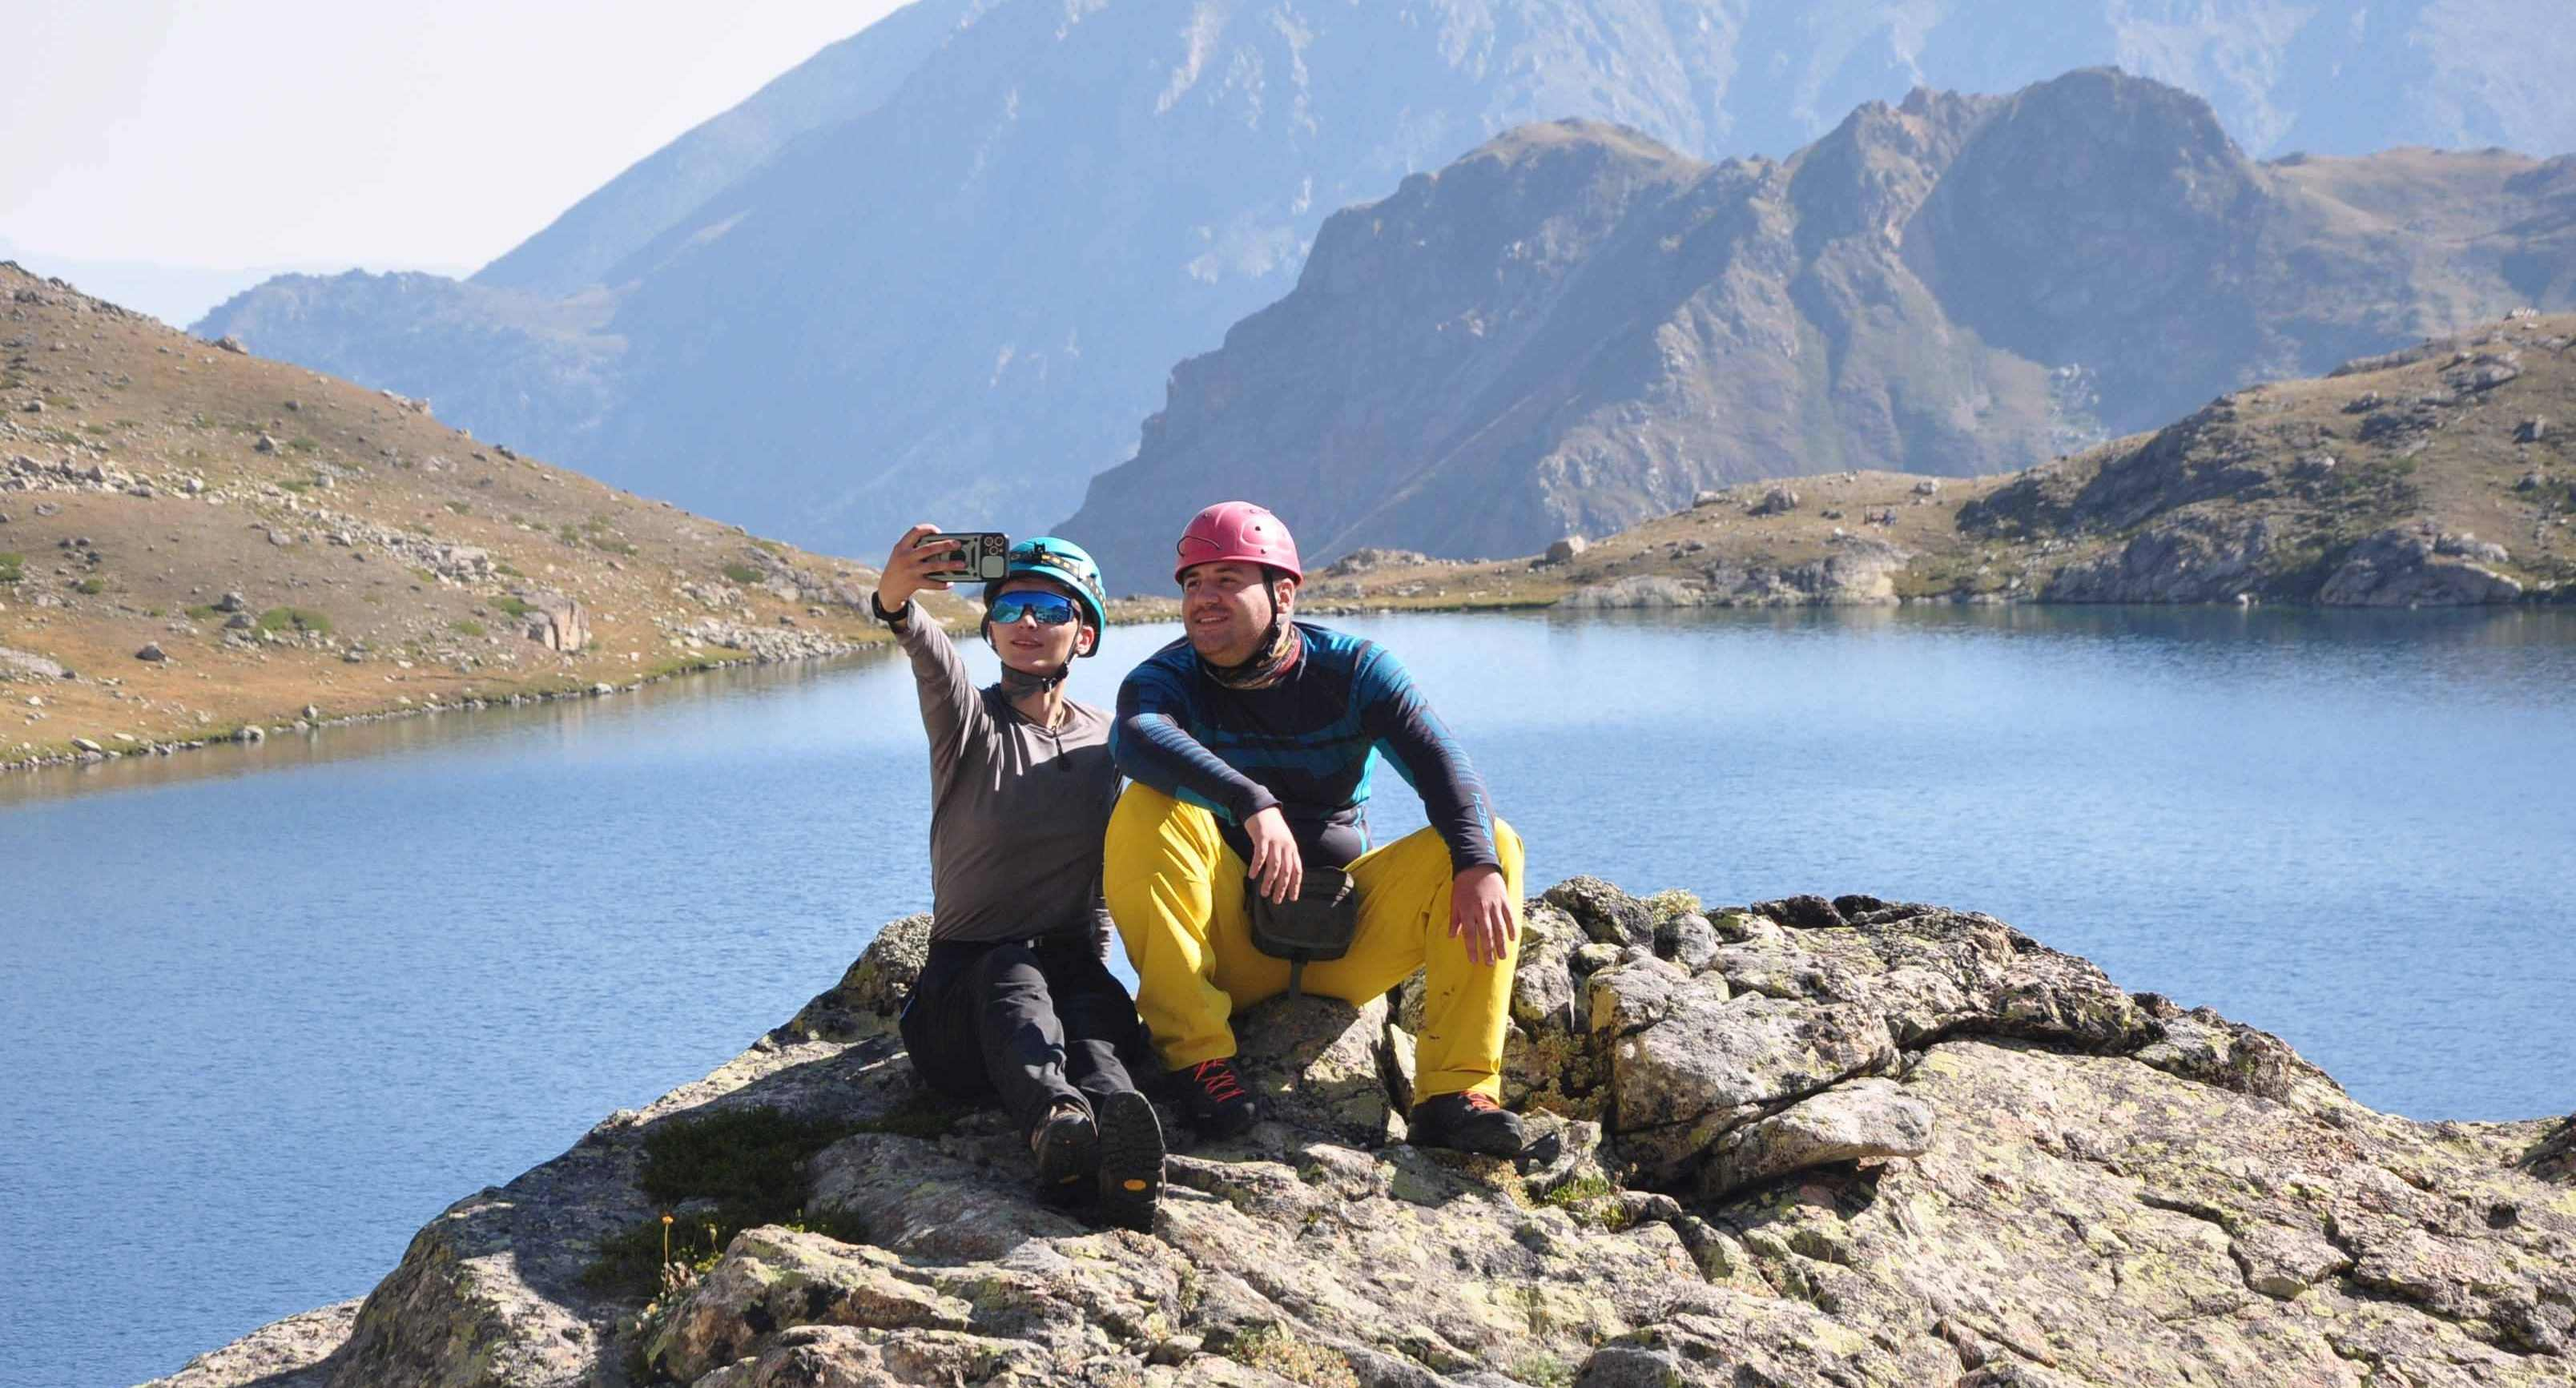
\includegraphics[width=0.7\linewidth]{../pics/DSC_0907}
	\caption{Фоткаемся на фоне озера}
	\label{fig:DSC_0907}
\end{figure}

\begin{figure}[h!]
	\centering
	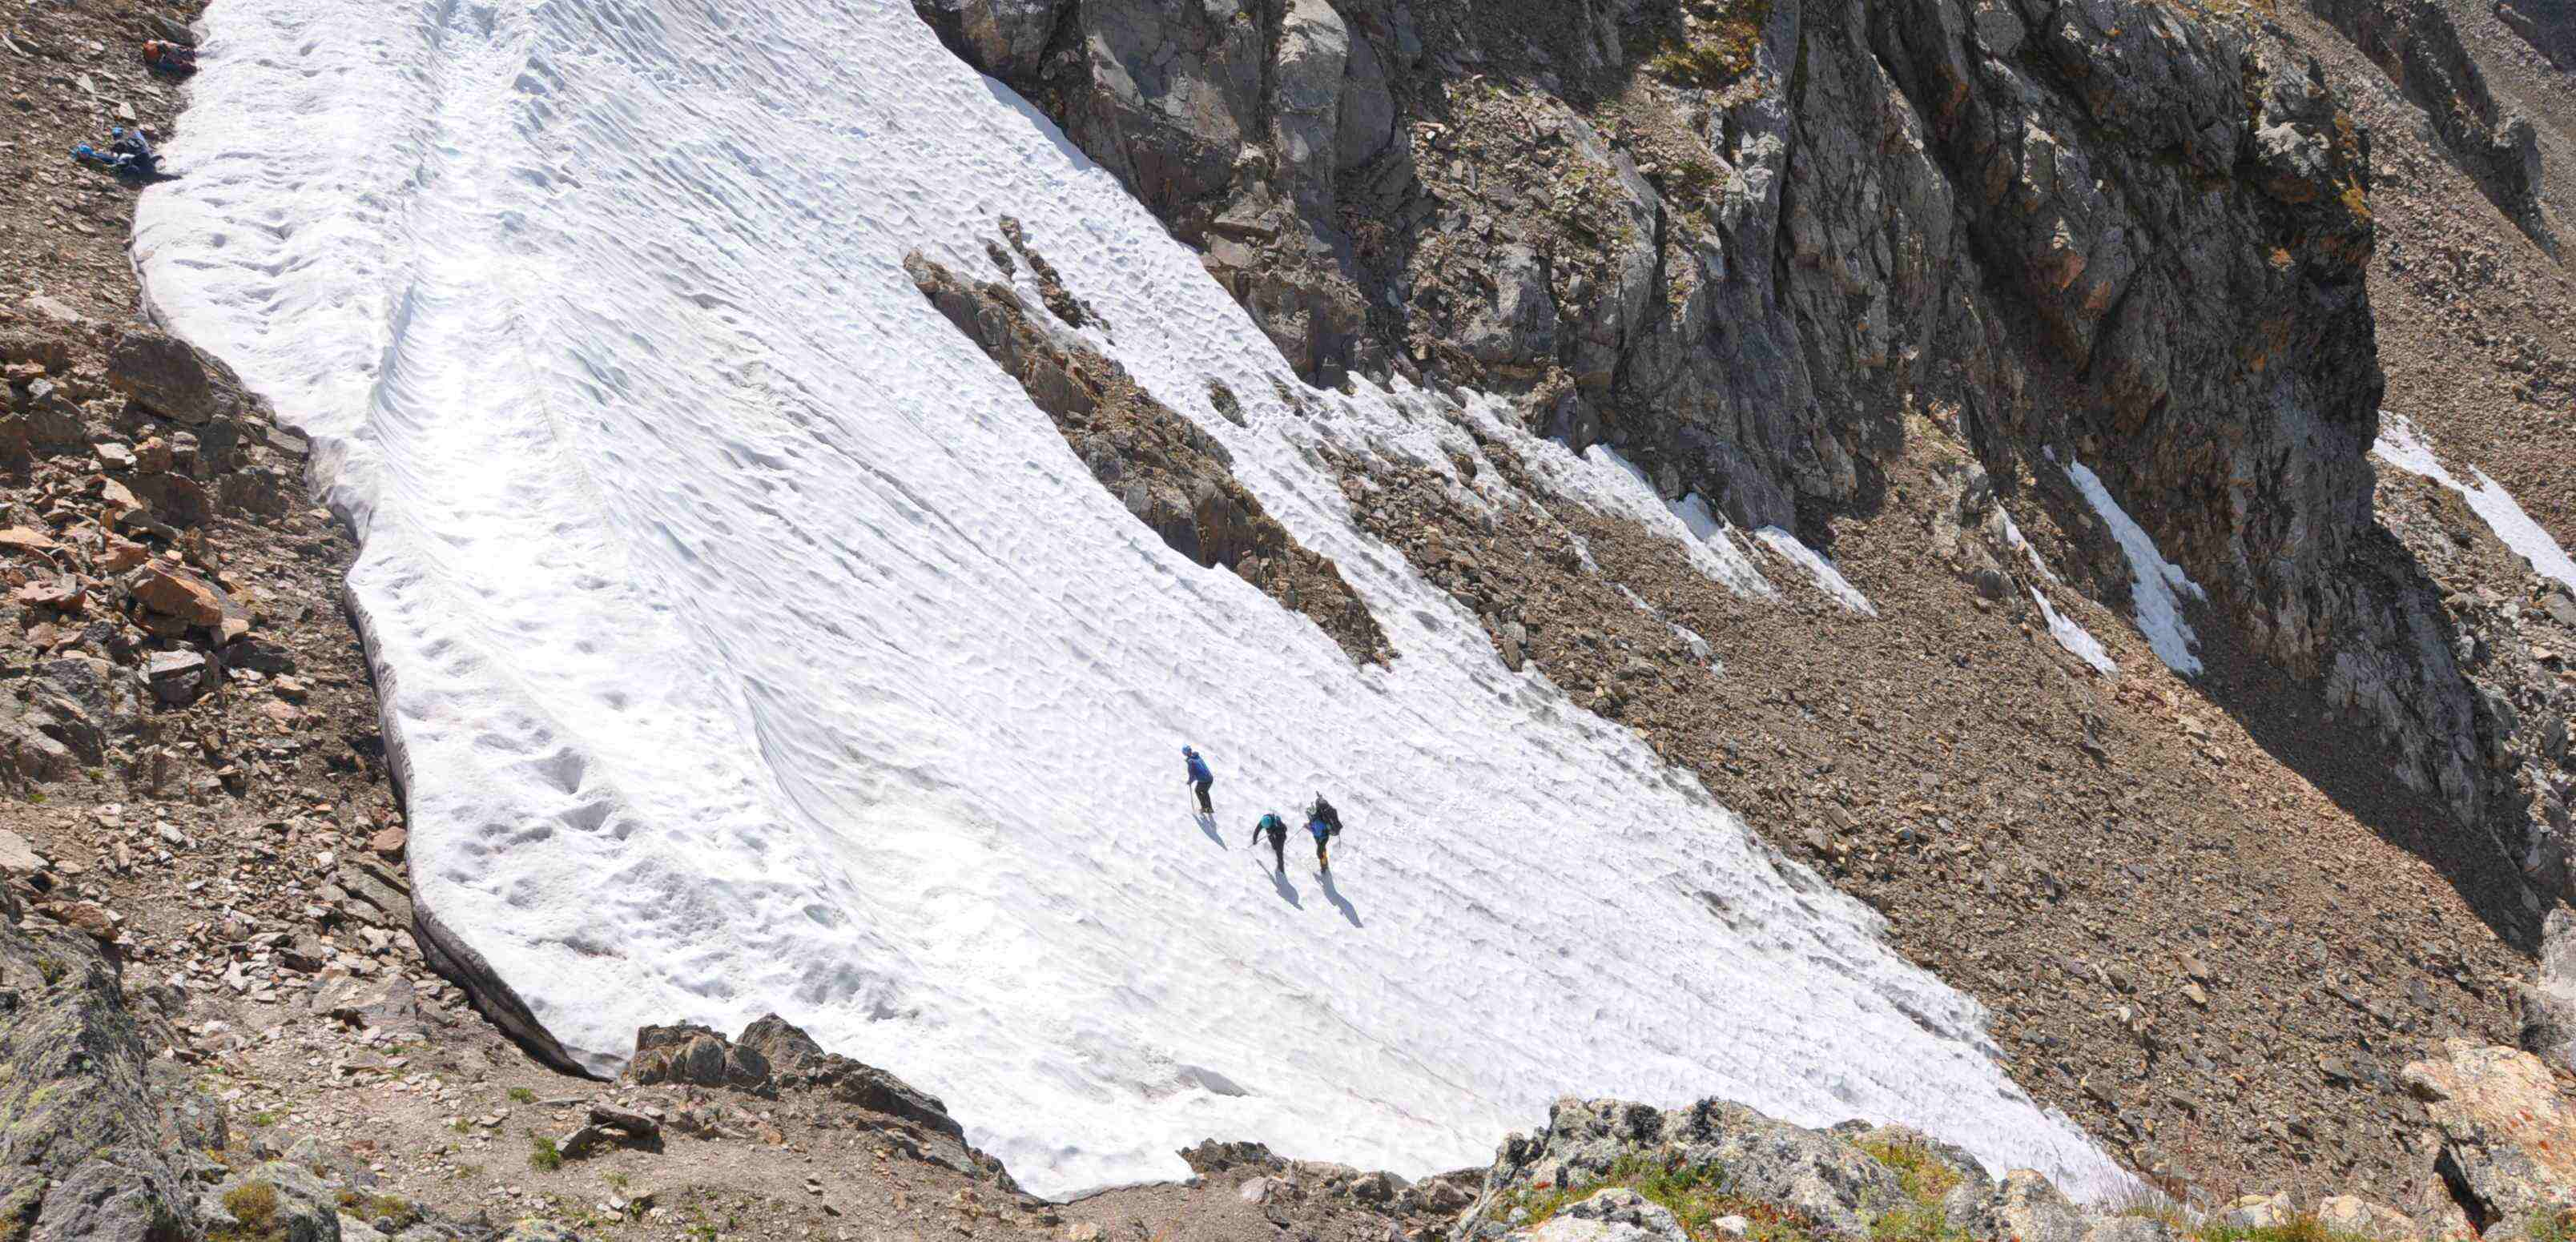
\includegraphics[width=0.7\linewidth]{../pics/DSC_0946.png}
	\caption{Маршрут движения группы по снежнику (красный), траектория срыва участника (синий), маршрут подъёма с сорвавшимся участником (чёрный)}
	\label{fig:DSC_0946}
\end{figure}


\begin{figure}[h!]
	\centering
	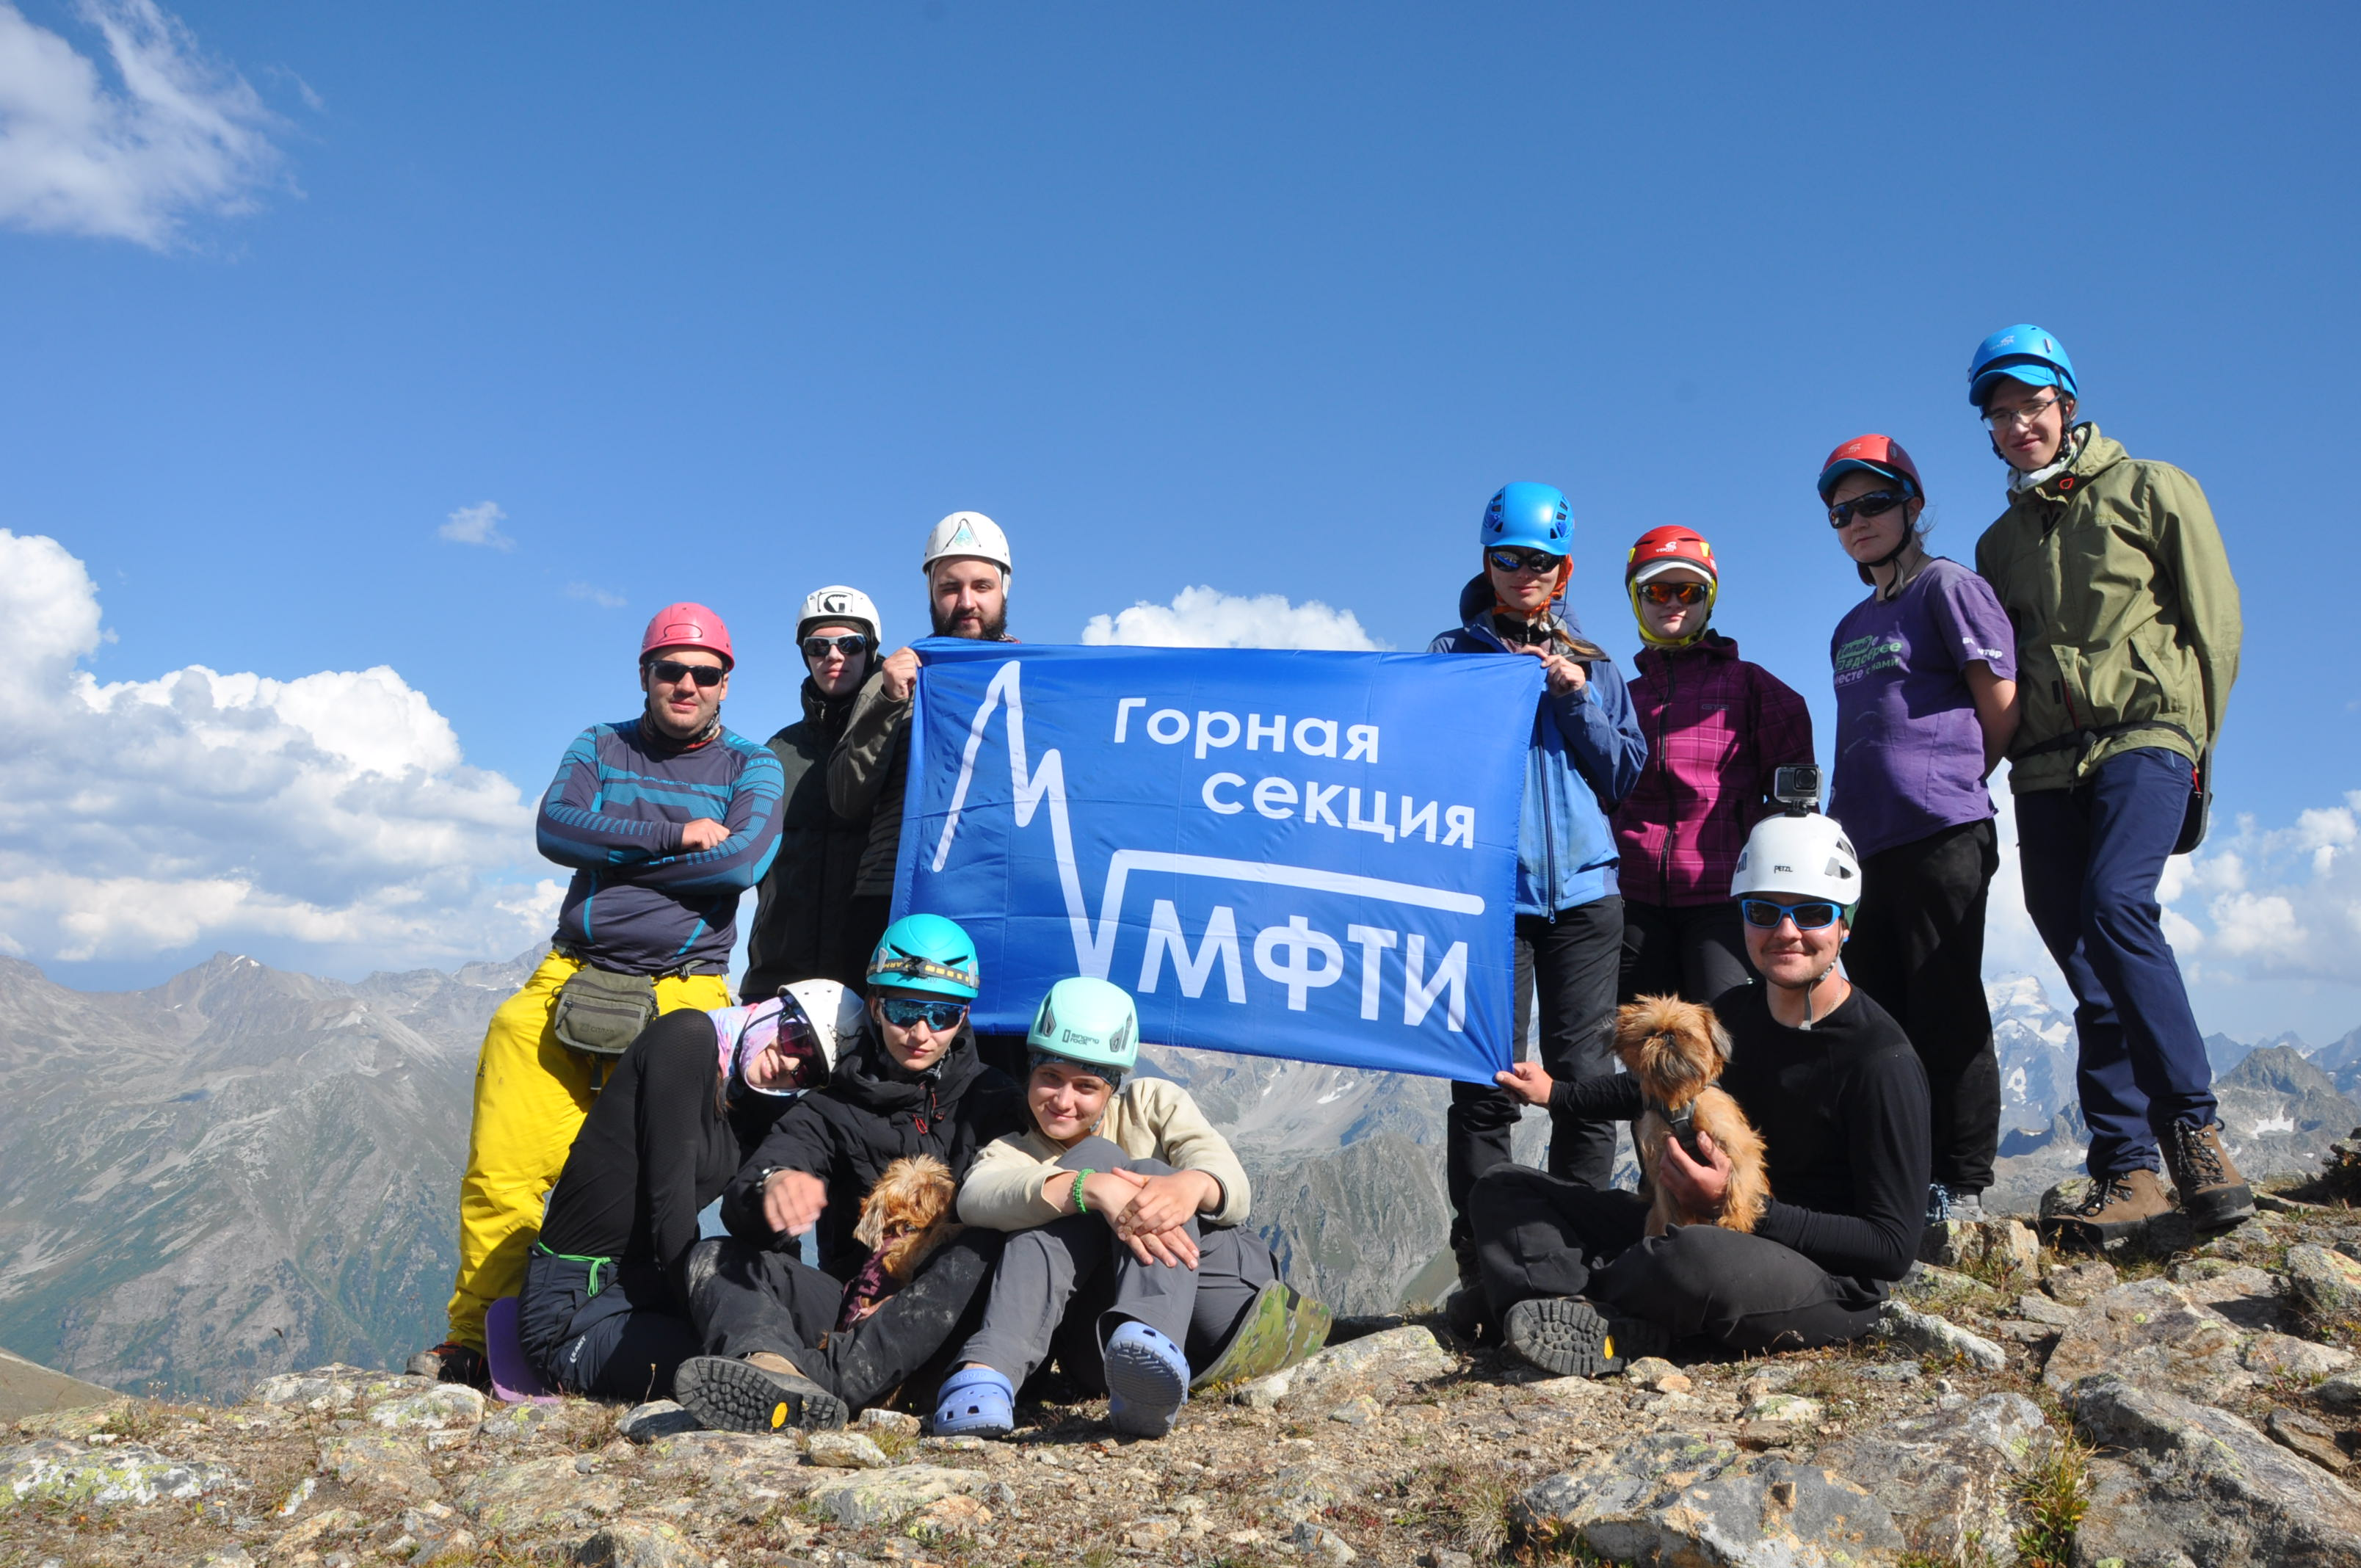
\includegraphics[width=0.7\linewidth]{../pics/DSC_0982}
	\caption{Группа на перевале, вид на д.р. Махар}
	\label{fig:DSC_0982}
\end{figure}

\begin{figure}[h!]
	\centering
	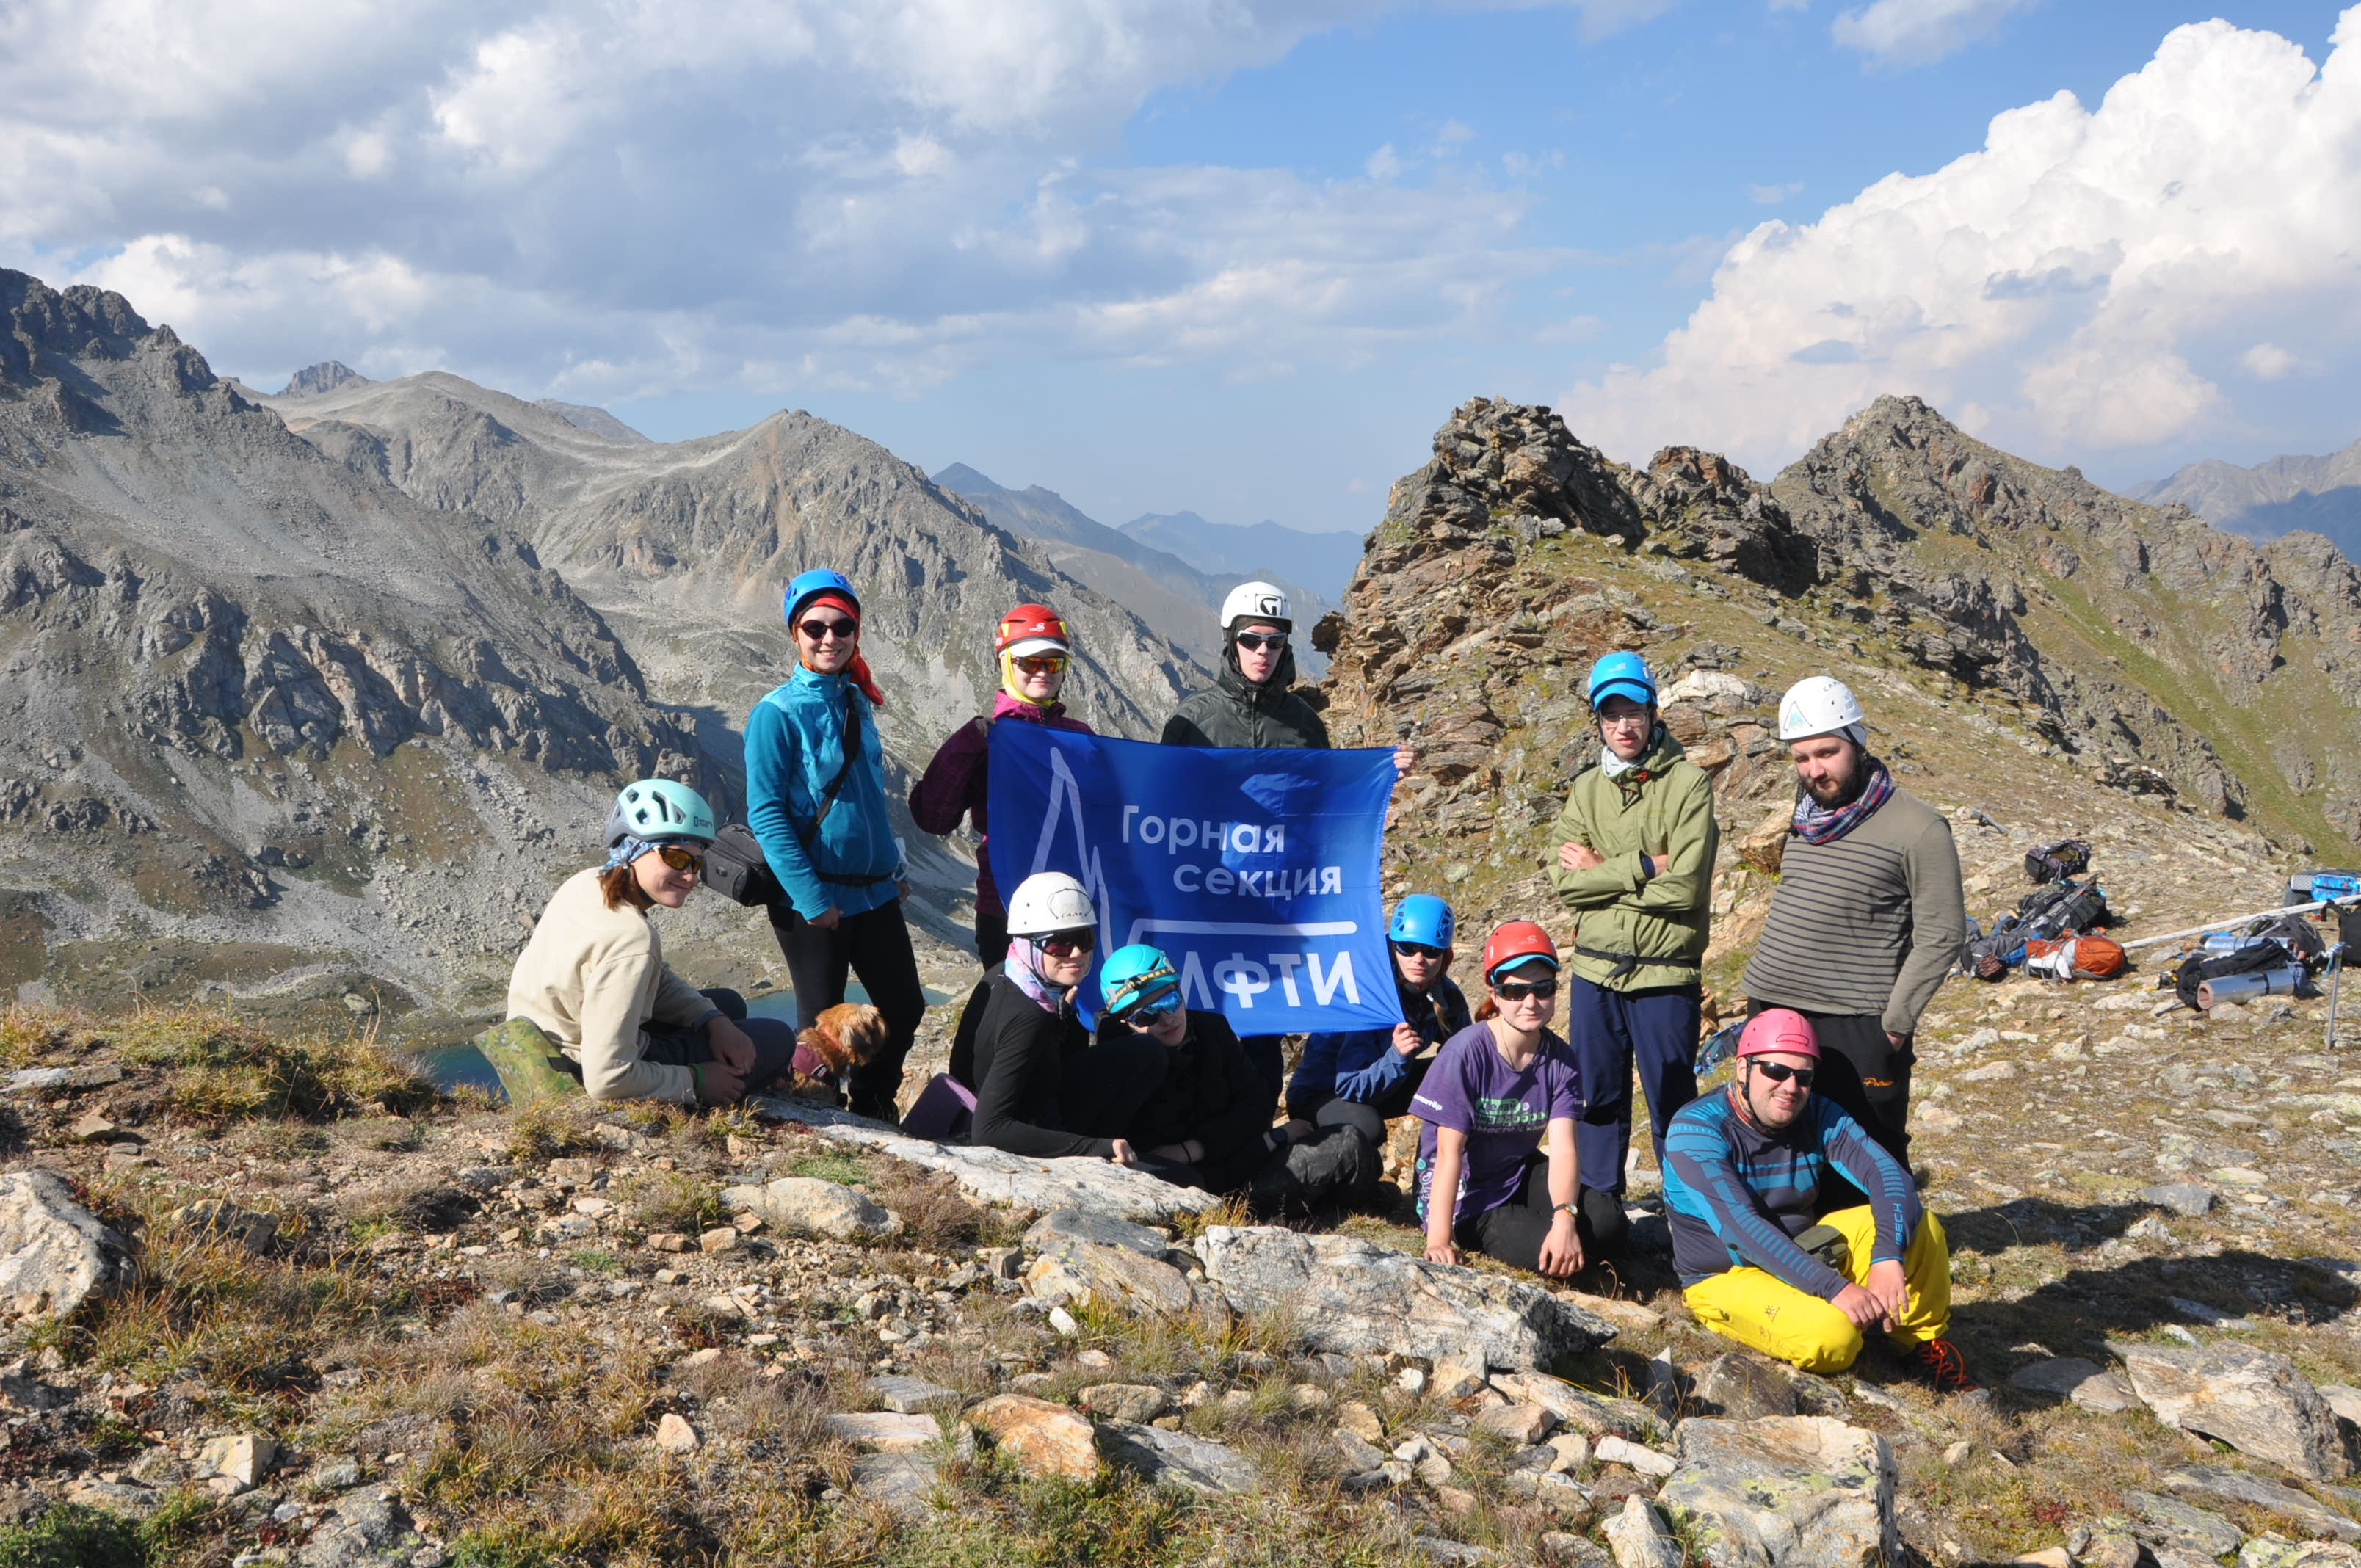
\includegraphics[width=0.7\linewidth]{../pics/DSC_0986}
	\caption{Группа на перевале, вид на оз. Уллу-Кёль}
	\label{fig:DSC_0986}
\end{figure}

\newpage
\subsection{21 августа. Т/б <<Глобус>>}
\textbf{Примечание: в приложении есть описание этого дня от одного из участников похода, Ильи Шалфеева. \ref{ilya}}

\textit{Метеоусловия: утром, днём, вечером ясно, тепло}

\begin{figure}[h!]
	\centering
	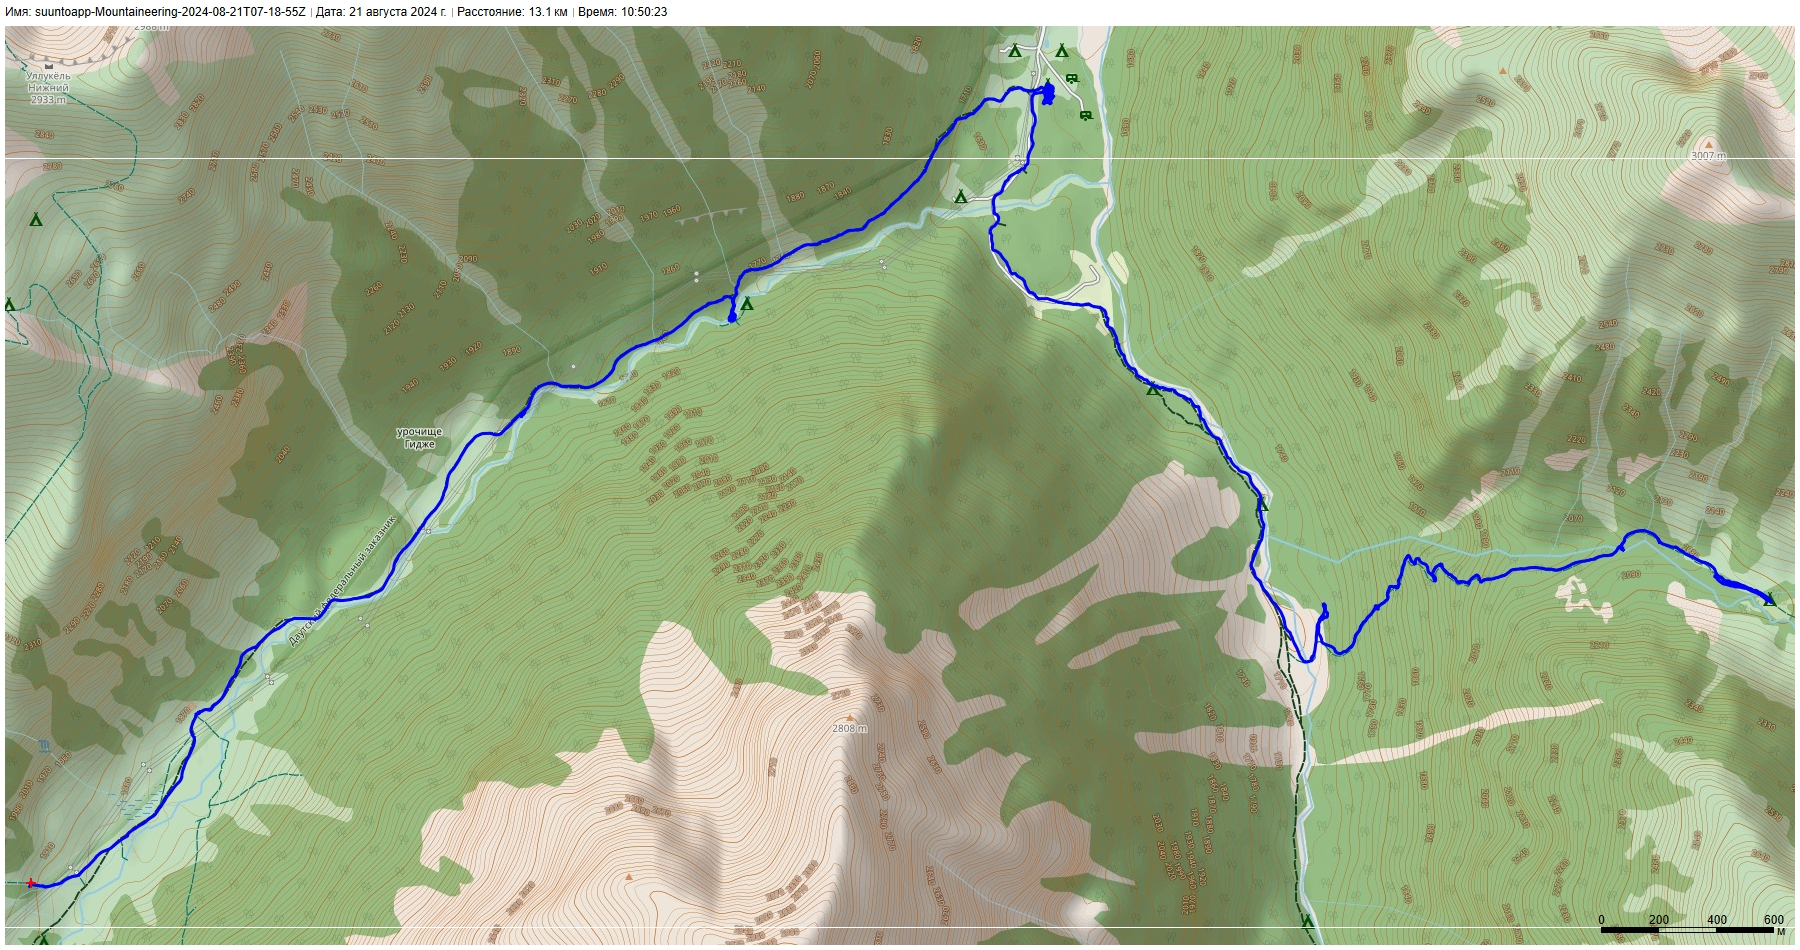
\includegraphics[angle=0, width=0.7\linewidth]{../pics/mini_maps/21}
	\label{fig:mini_21}
\end{figure}

Подъём дежурных между 07:00 и 08:00; общий подъём в 08:30. (рис.~\ref{fig:DSC_0993}). 

\begin{figure}[h]
	\centering
	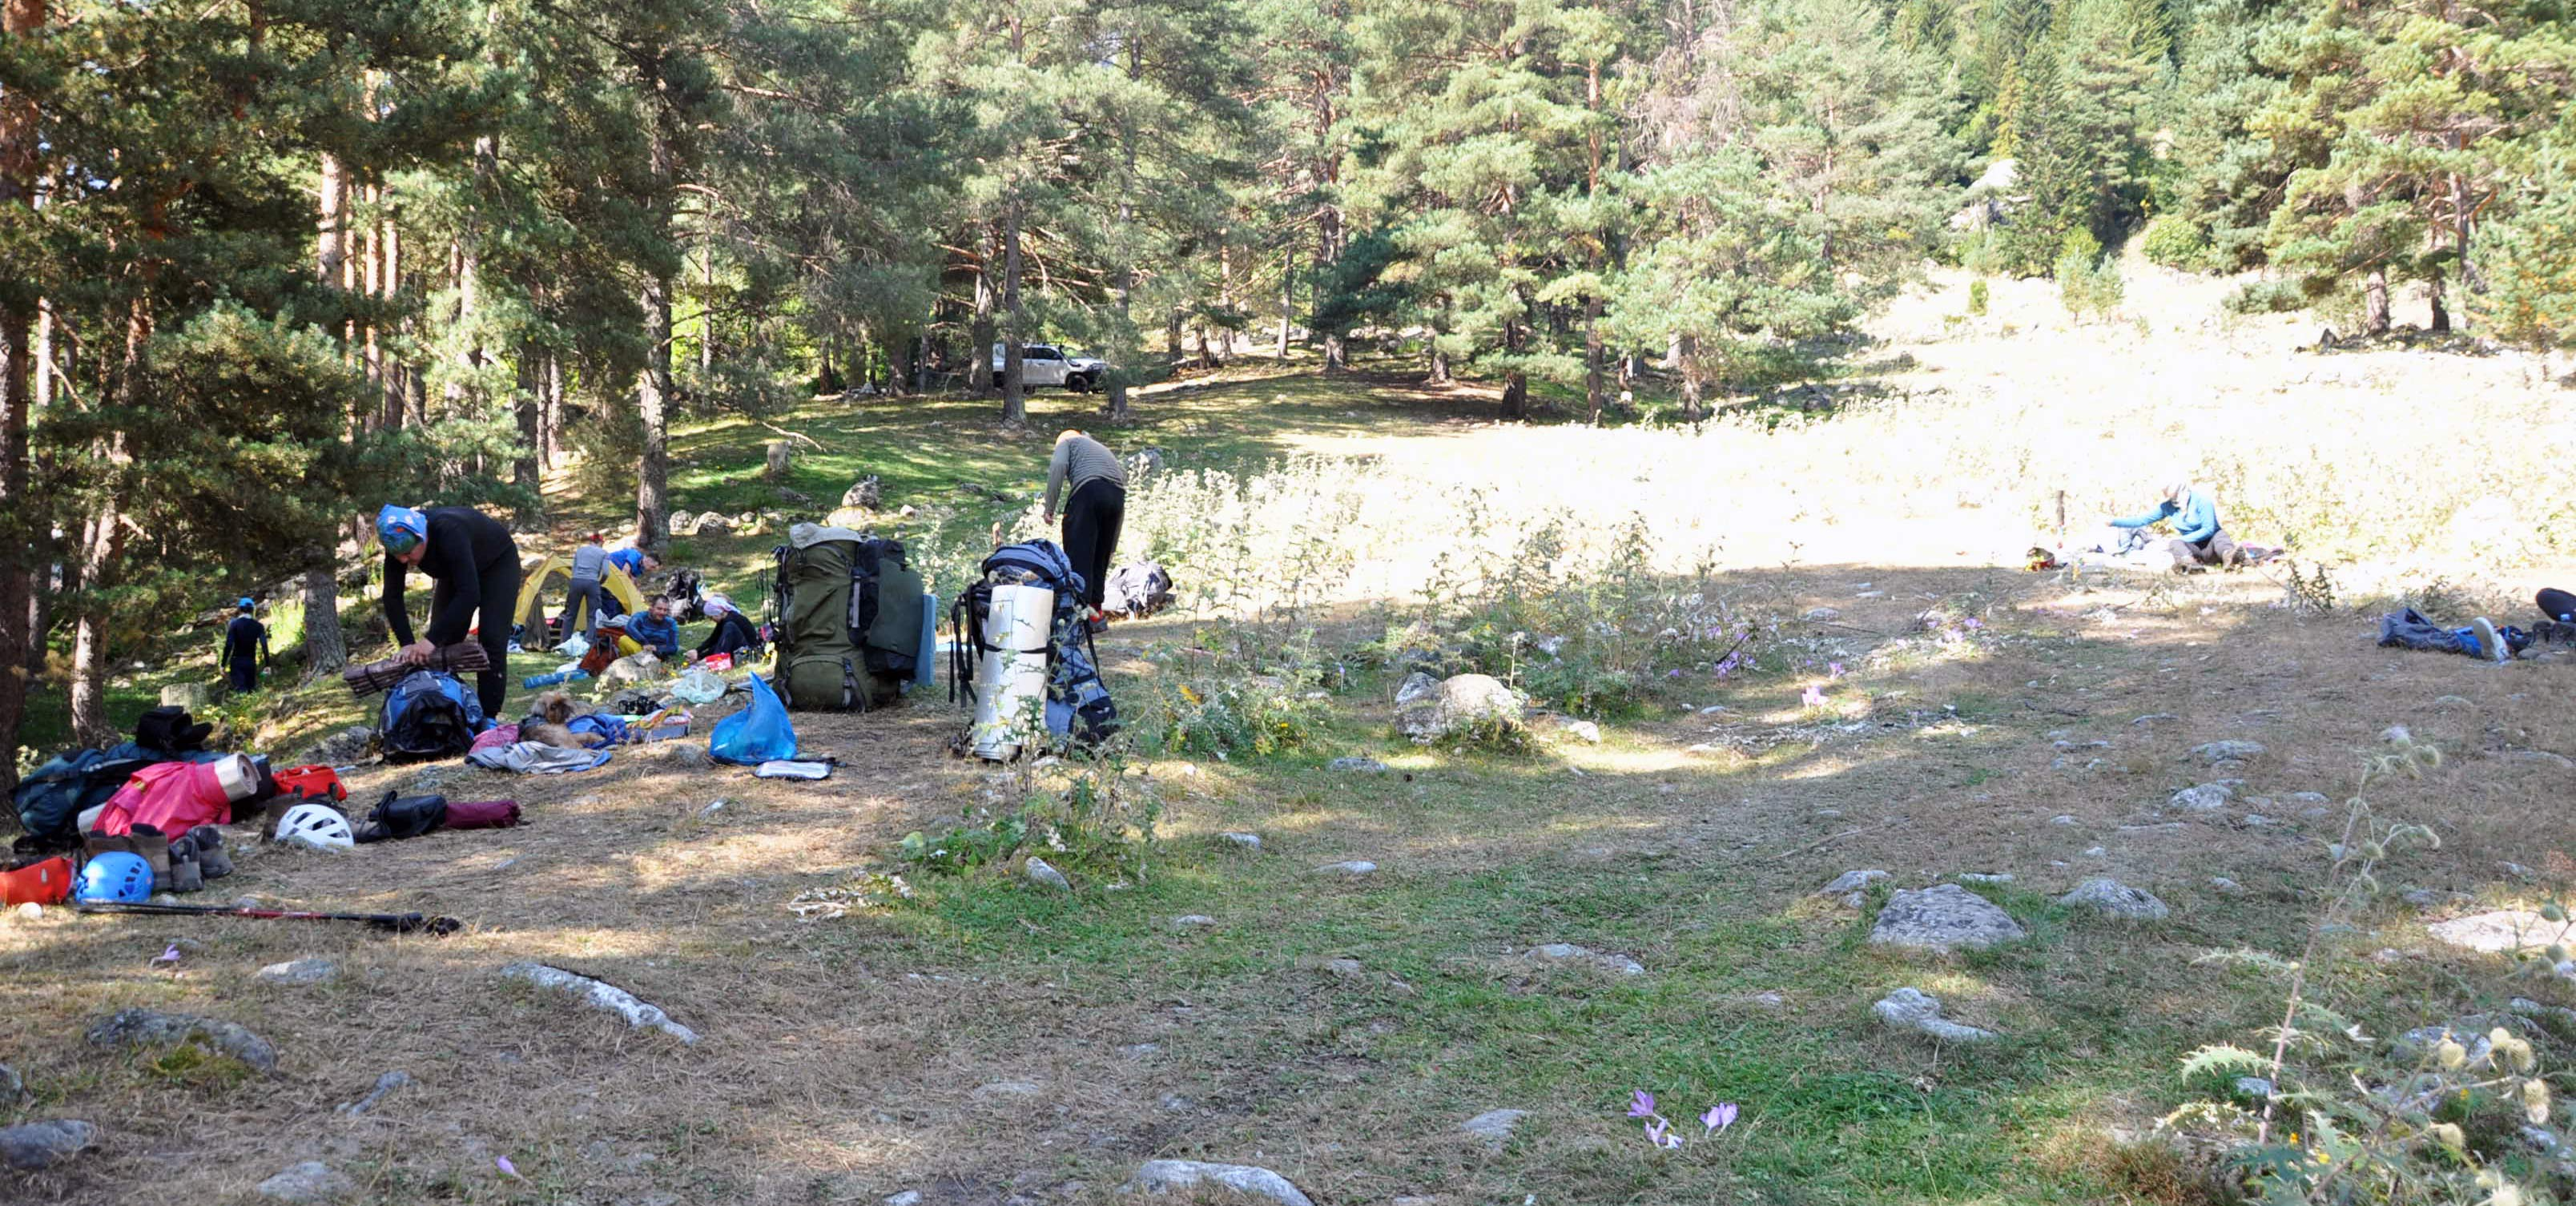
\includegraphics[width=0.7\linewidth]{../pics/DSC_0993}
	\caption{м.н. 20-21 августа}
	\label{fig:DSC_0993}
\end{figure}

Не спеша позавтракали, отдыхая от позднего завершения вчерашнего дня, и в 10:20 выдвинулись по д.р. Махар в сторону т/б <<Глобус>>(рис.~\ref{fig:DSC_1003}). 

\begin{figure}[h]
	\centering
	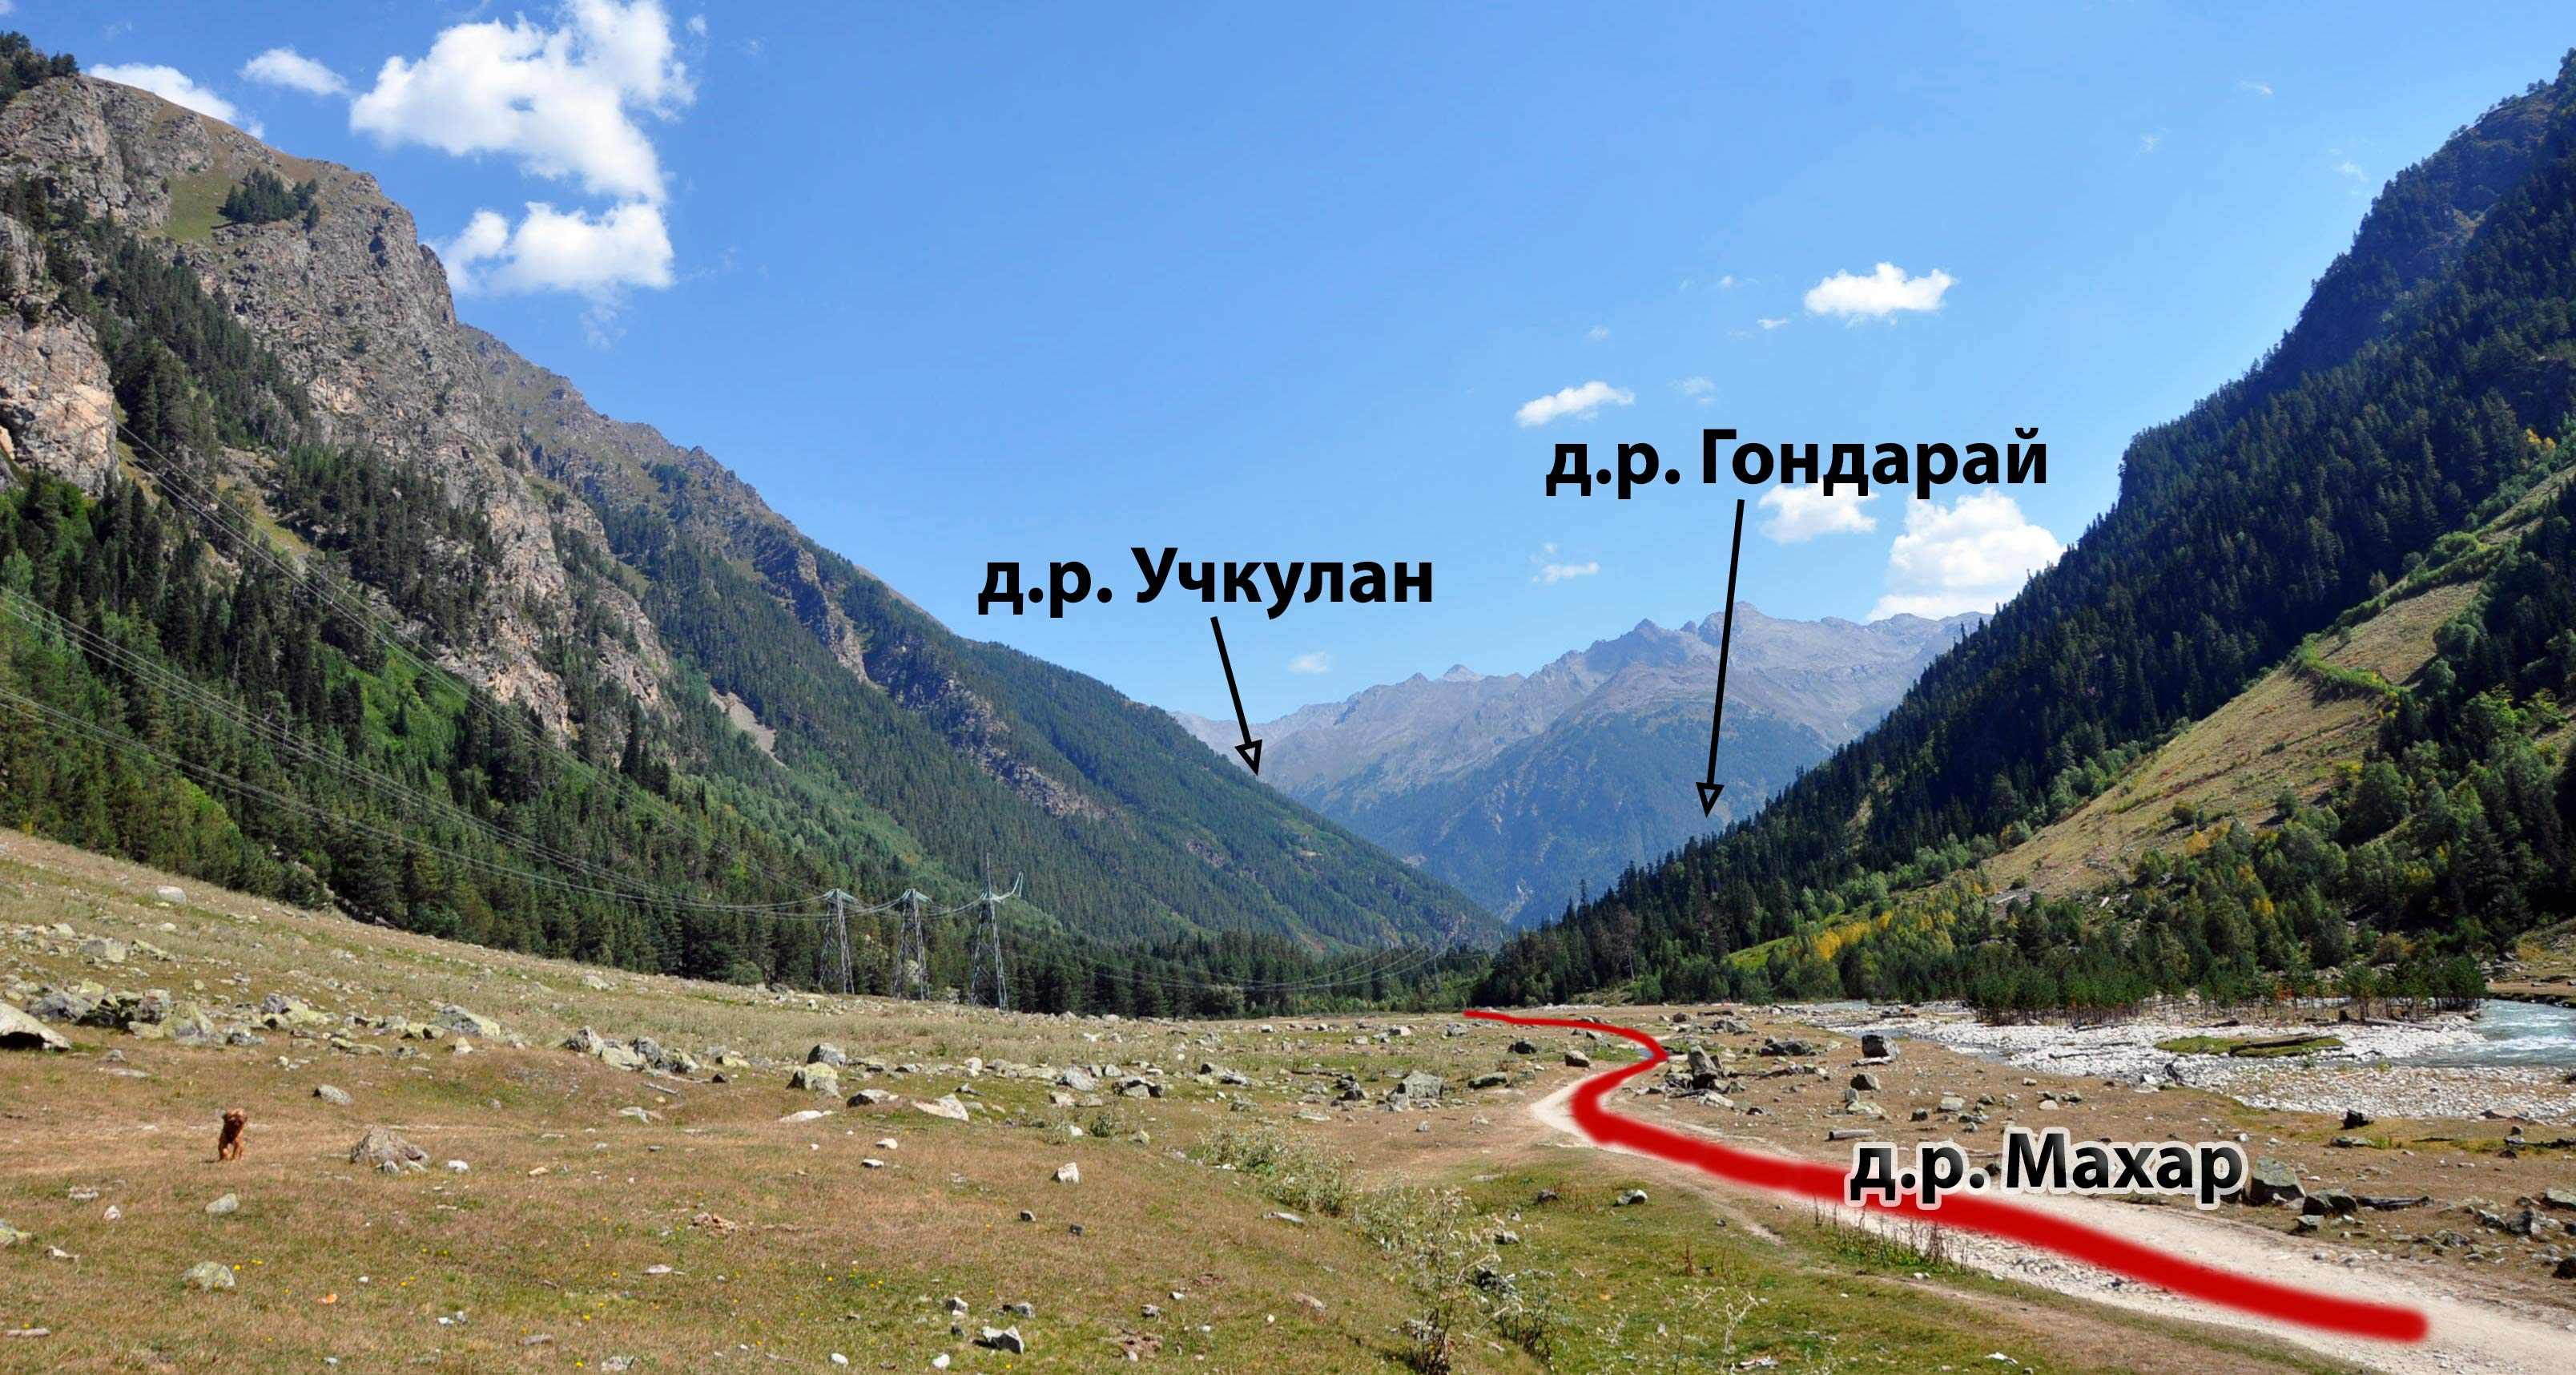
\includegraphics[width=0.7\linewidth]{../pics/DSC_1003}
	\caption{м.н. 20-21 августа}
	\label{fig:DSC_1003}
\end{figure}

Через 20~мин ЧХВ подошли к посту пограничников. Пограничники задали нам вопросы о направлении движения, сфотографировали нитку маршрута в маршрутной книжке, но документы не проверили. Выйдя от них, ещё через 22~мин ЧХВ дошли до нарзанных источников (находятся на правом берегу р. Махар, туда ведёт хороший подвесной мост, рис.~\ref{fig:DSC_1043}). Координаты источников: N43.312198\degree,\\E43.312198\degree.

\begin{figure}[h!]
	\centering
	\begin{minipage}[h]{0.62\linewidth}
		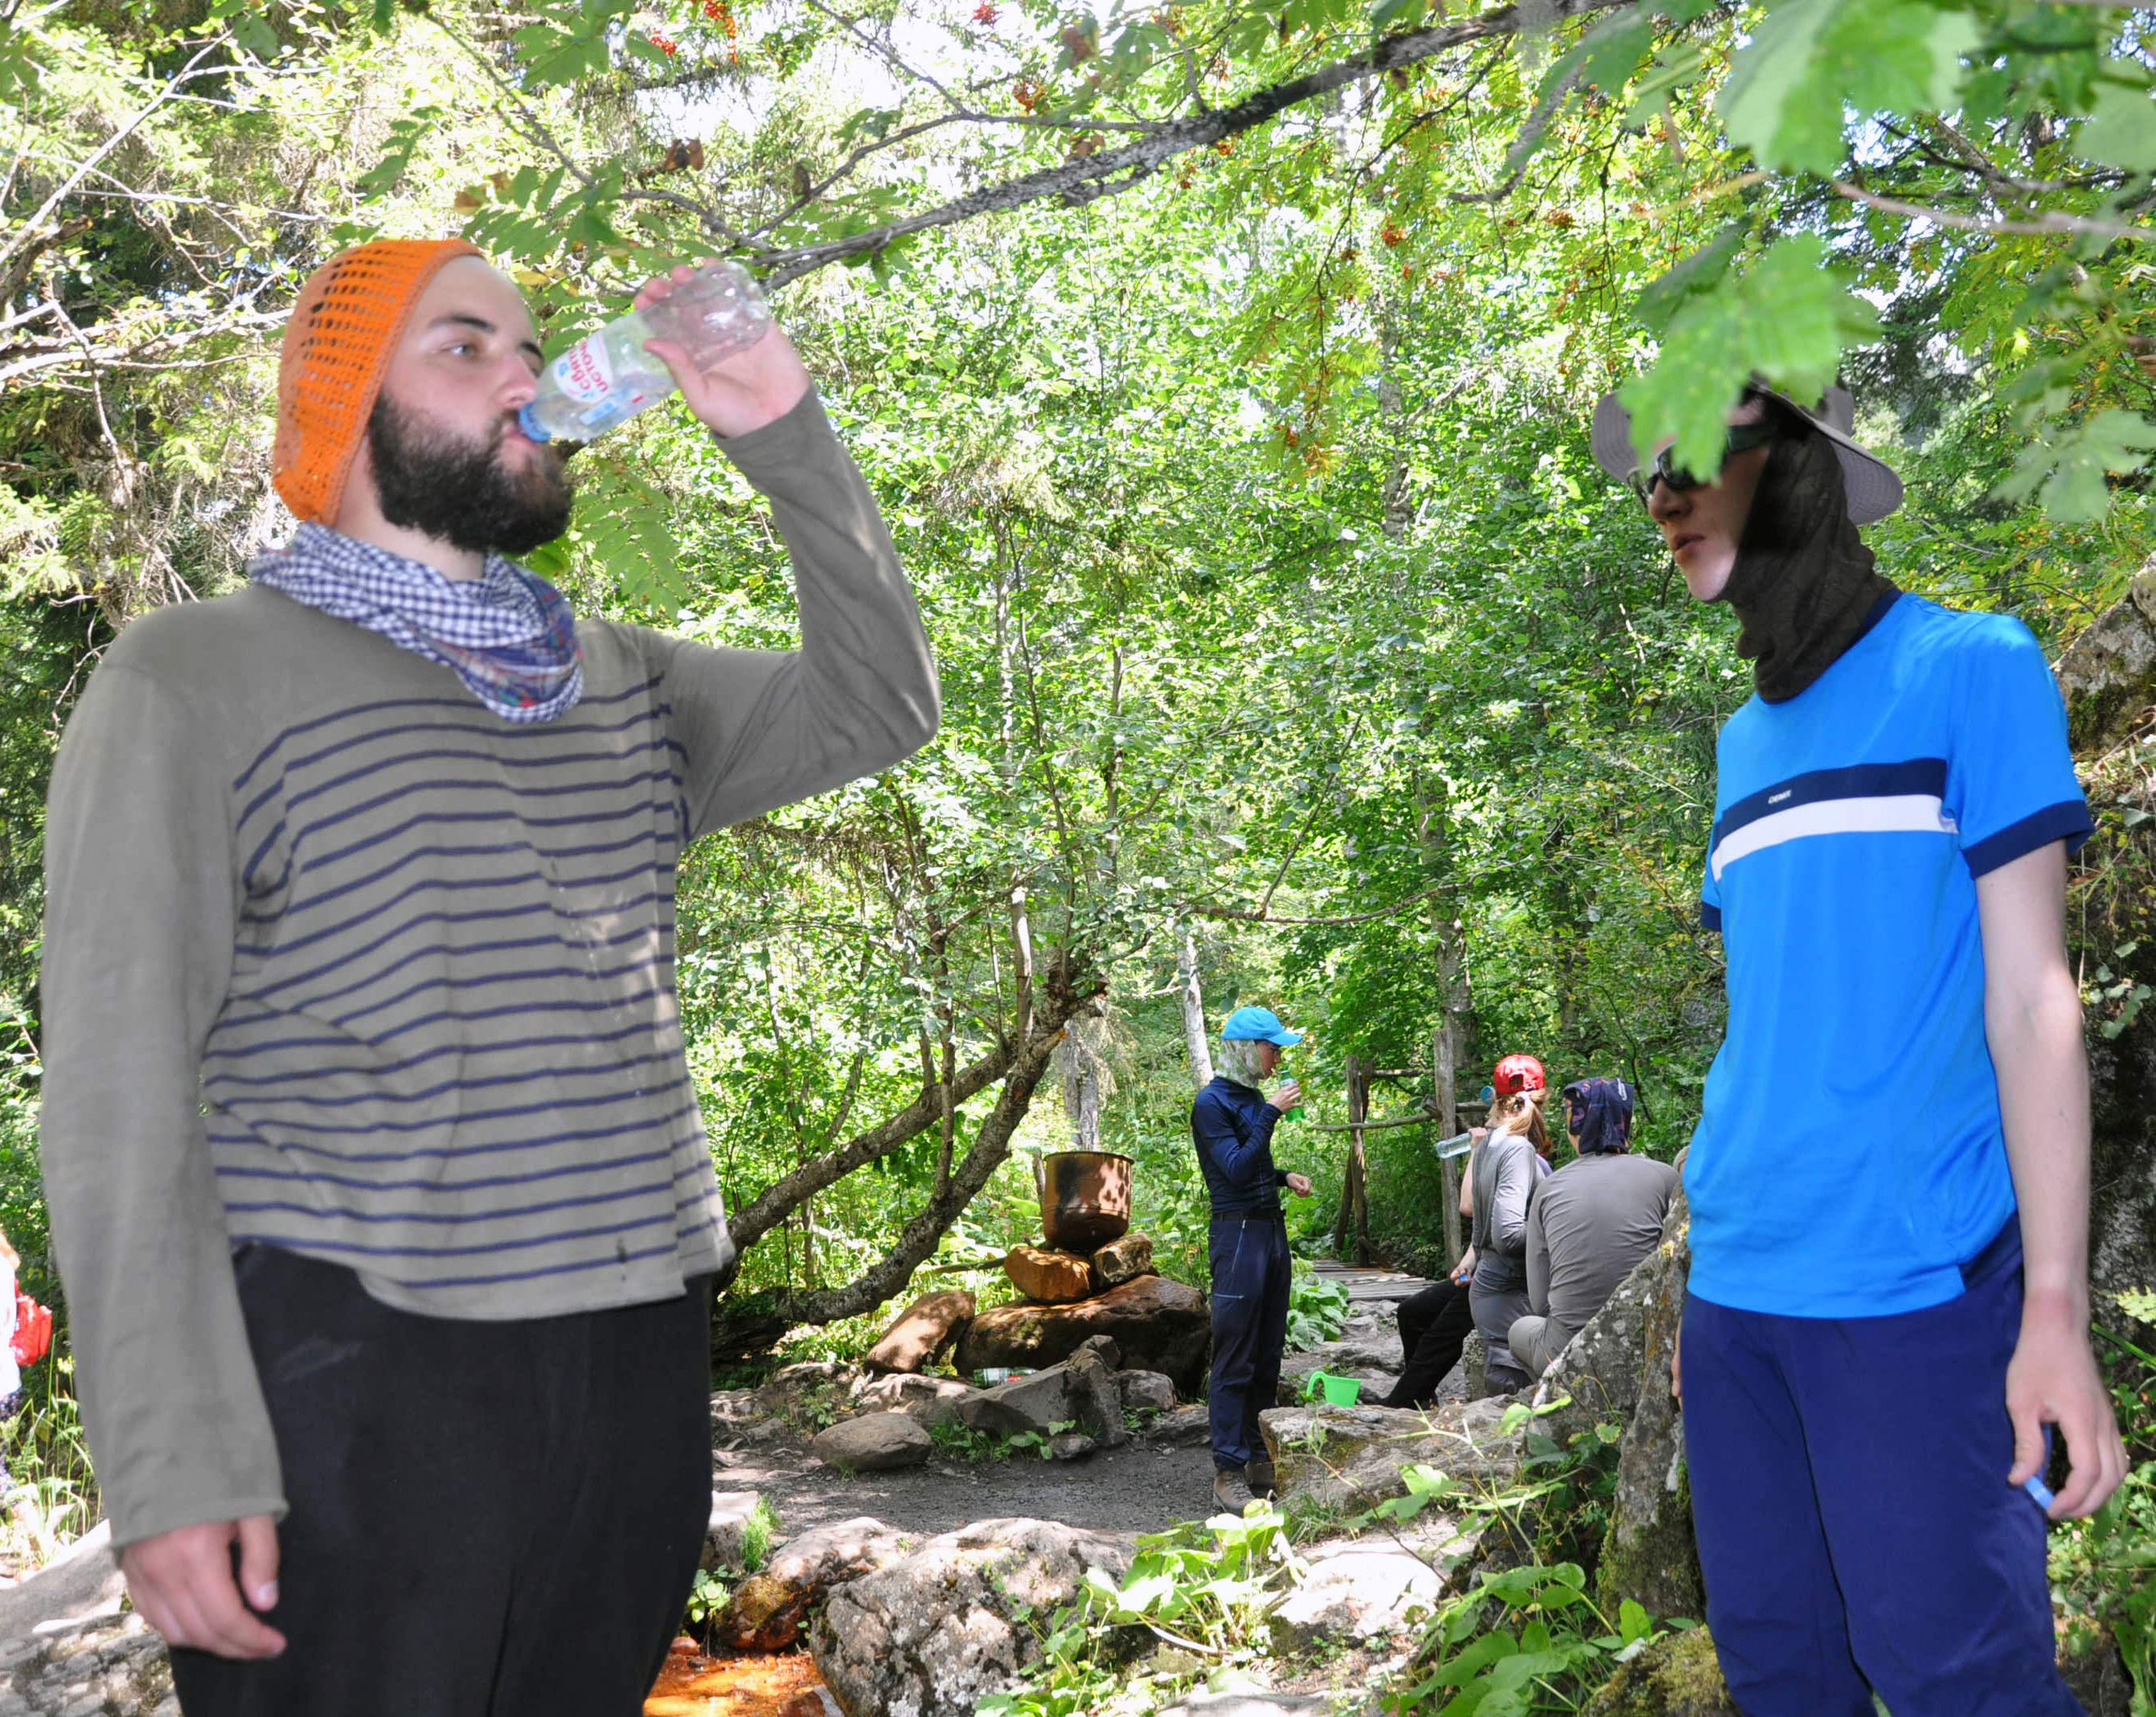
\includegraphics[width=\linewidth]{../pics/DSC_1043.jpg}
	\end{minipage}
	\quad
	\begin{minipage}[h]{0.35\linewidth}
		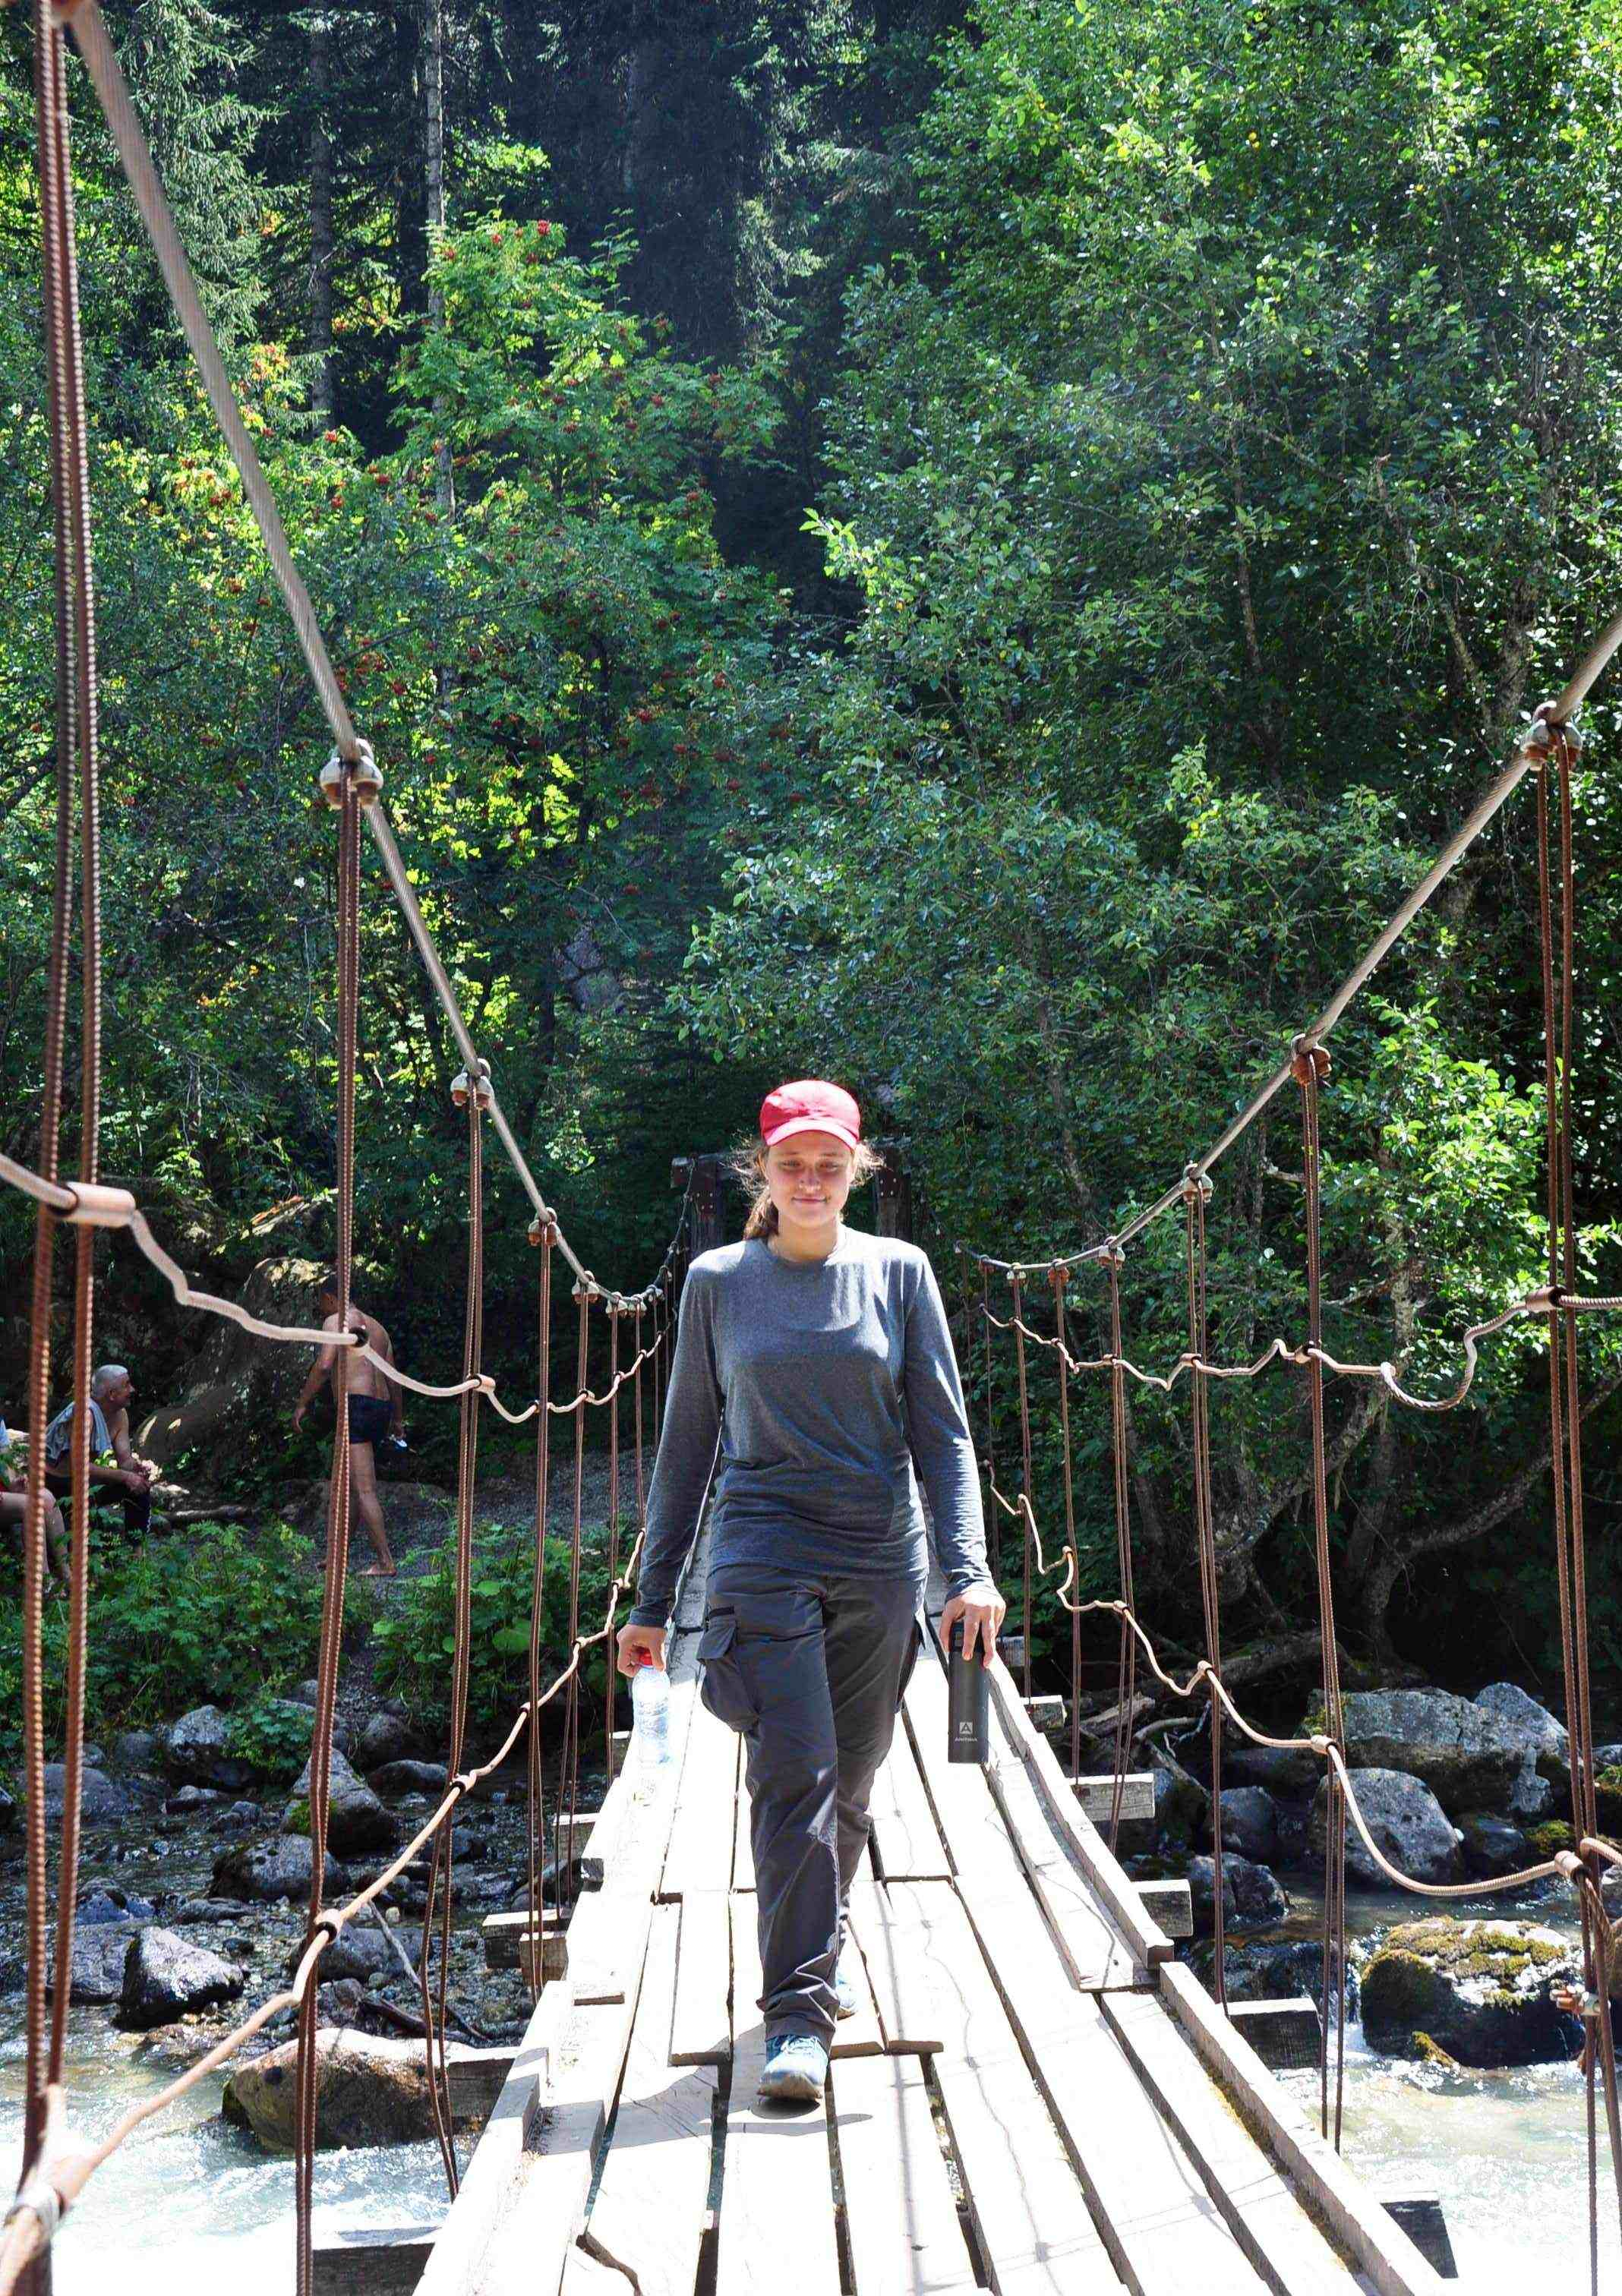
\includegraphics[width=\linewidth]{../pics/DSC_1098.jpg}
	\end{minipage}
	\caption{Слева: группа на нарзанных источниках. Справа: мост через р. Махар к источникам}
	\label{fig:DSC_1043}
\end{figure}

В 12:05 пришли в т/б <<Глобус>>, где встали на обед. Информация о благах цивилизации в турбазе: можно бесплатно подзарядить телефоны (около 5 шт одновременно, предположительно, что от солнечной батареи), при необходимости можно попросить Wi-Fi, с которого, если повезёт, получится обменяться парой сообщений с большой землёй. Также есть владелец одного из соседних кемпингов (по его собственным словам: есть подозрение, что это было не так), который за 300~\faRub~разрешил нам позвонить со своего телефона со стабильным интернетом. На территории турбазы есть душ, туалет, домики для ночлега и магазин с хычинами.

\begin{figure}[h!]
	\centering
	\begin{minipage}[h]{0.30\linewidth}
		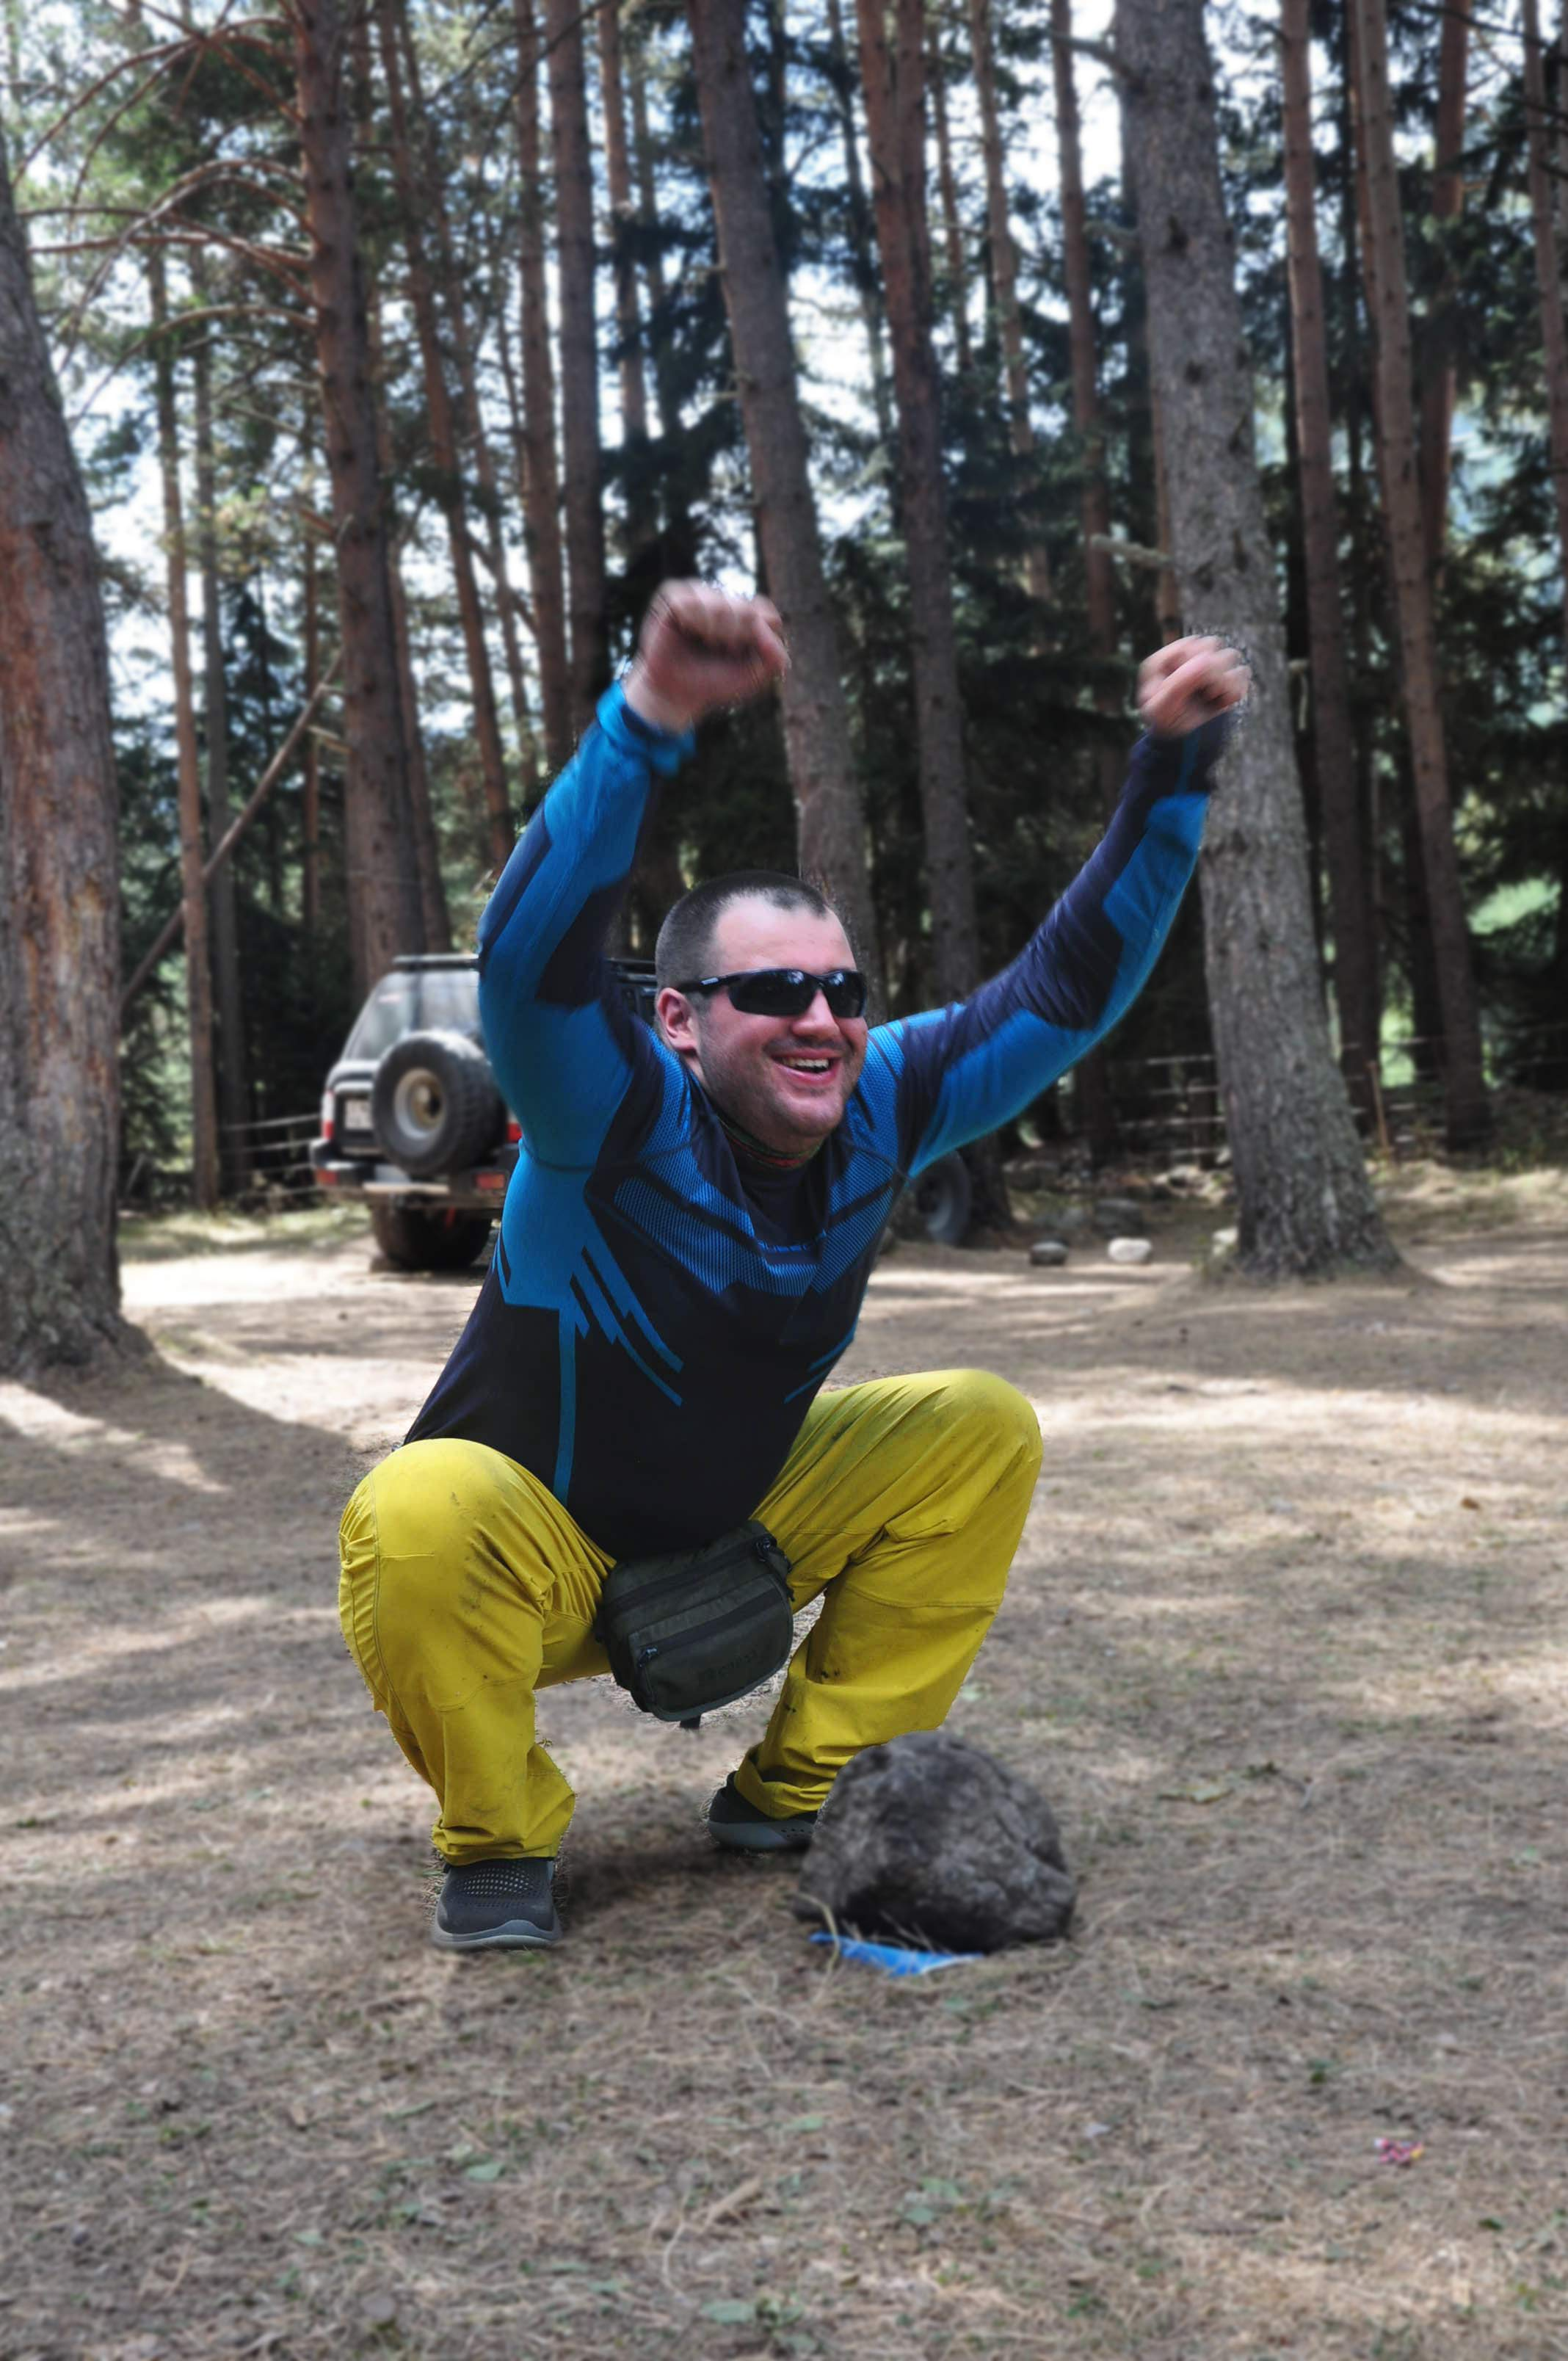
\includegraphics[width=\linewidth]{../pics/DSC_1150.jpg}
	\end{minipage}
	\quad
	\begin{minipage}[h]{0.30\linewidth}
		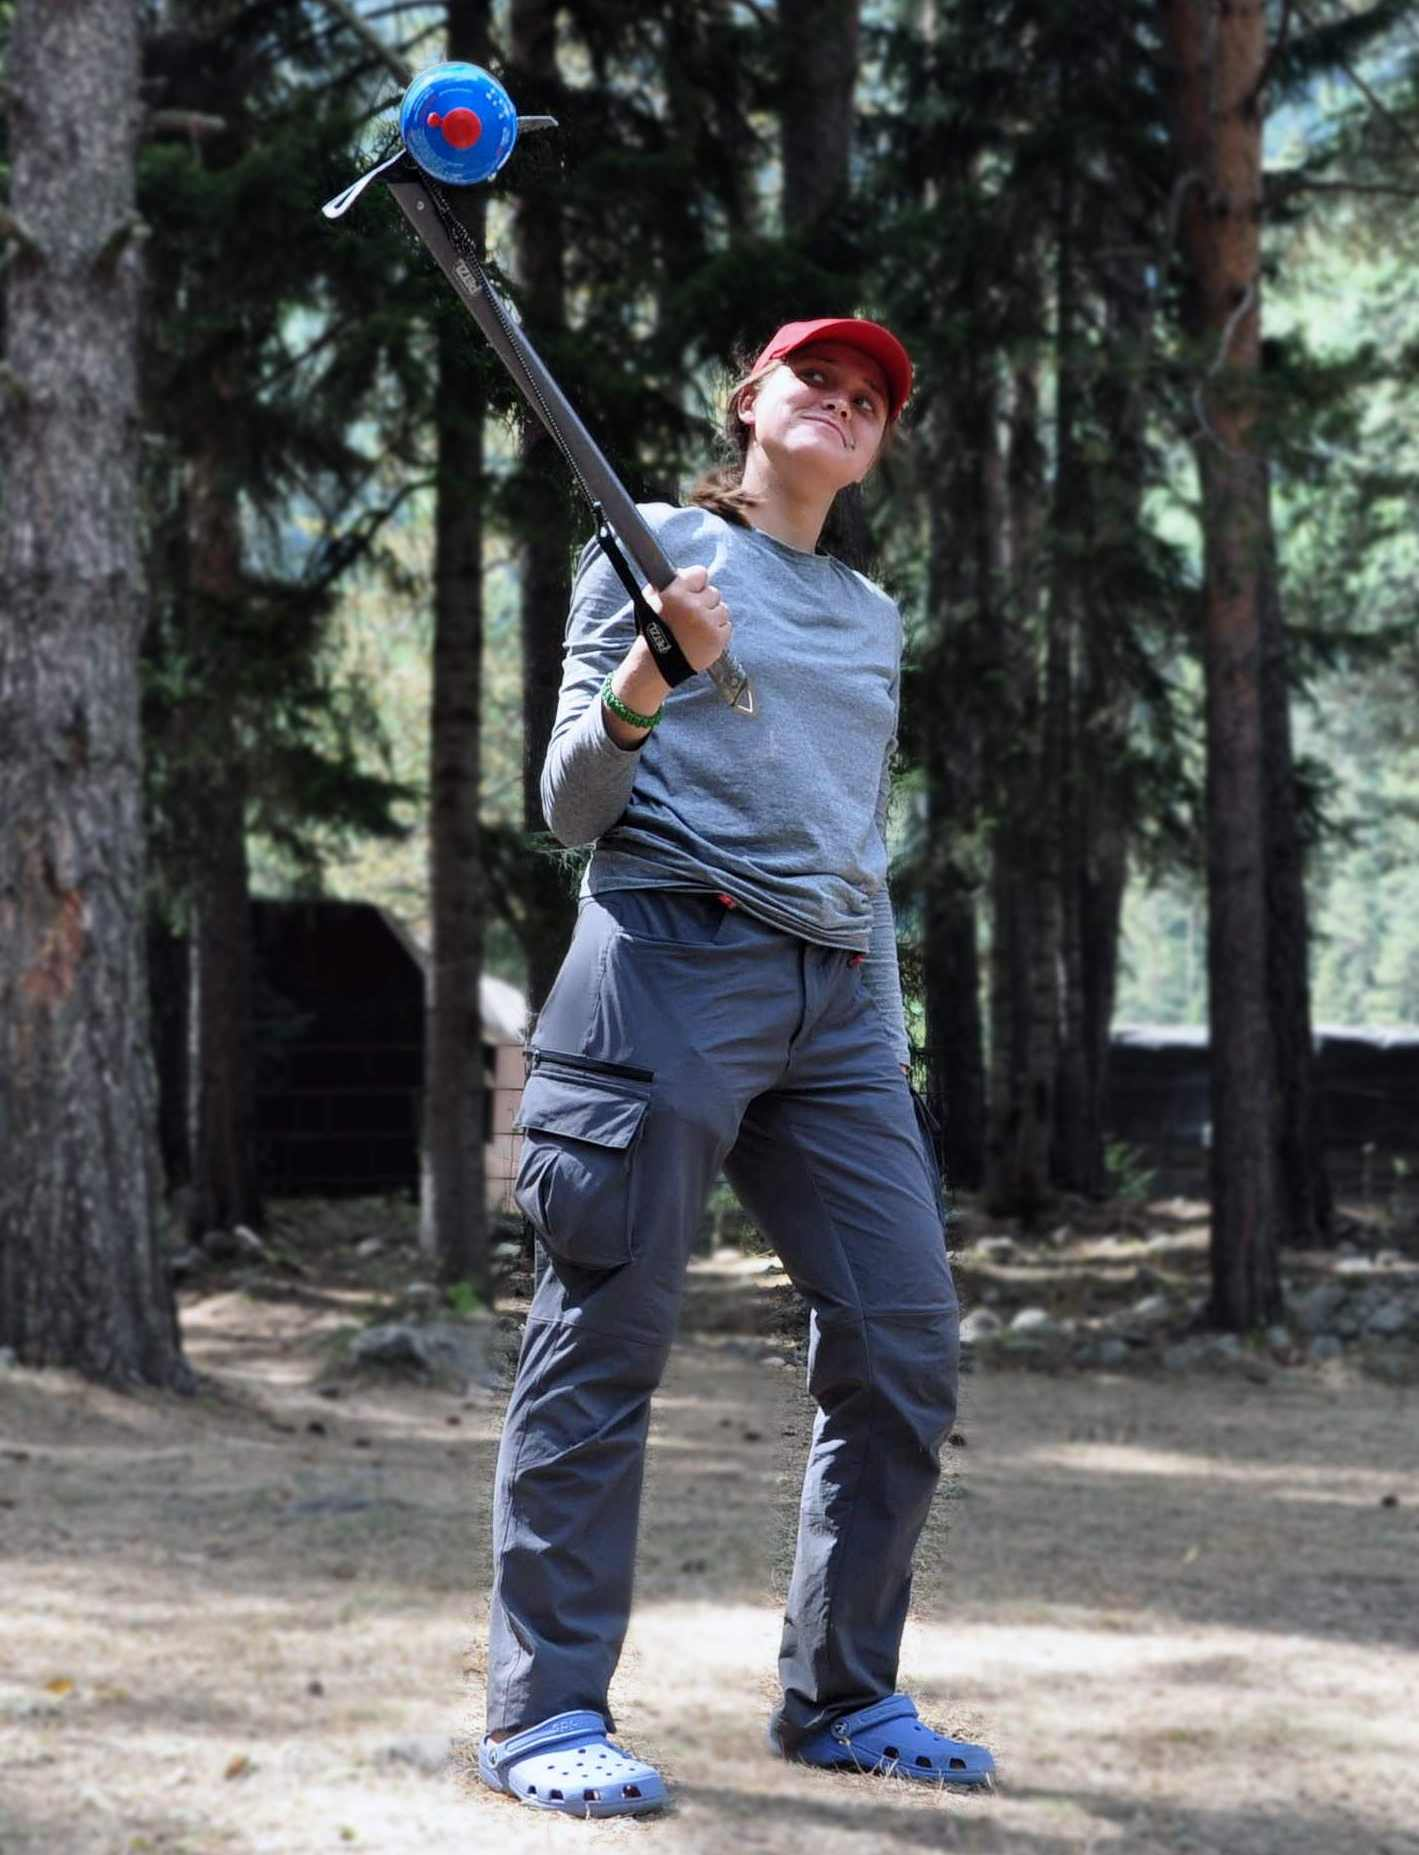
\includegraphics[width=\linewidth]{../pics/DSC_1152.jpg}
	\end{minipage}
	\caption{Учимся утилизировать использованные газовые баллоны \smiley}
	\label{fig:DSC_1150}
\end{figure}

После обеда один из участников, Георгий, сообщил группе о своём решении сойти с маршрута по причине того, что поход давался ему слишком тяжело: выявились проблемы с коленями, давлением, да и общий уровень физической подготовки, несмотря на то, что участник тренировался перед походом, оказался всё же недостаточным. На переходе до турбазы он обратился с этим к руководителю лично, и вовремя обеда вопрос обсуждался в личном порядке. Основной вклад в решение технических вопросов вносил при этом замруководителя. Довольно много времени ушло на обеспечение логистики Георгия на большую землю, и в 17:53 мы выдвинулись из турбазы по хорошей автомобильной дороге по правому берегу р. Учкулан. В 18:06 пересекли р. Махар по хорошему автомобильному мосту., а в 18:32~--- р. Гондарай по трём хорошим брёвнам (рис.~\ref{fig:hondaray}).

\begin{figure}[h]
	\centering
	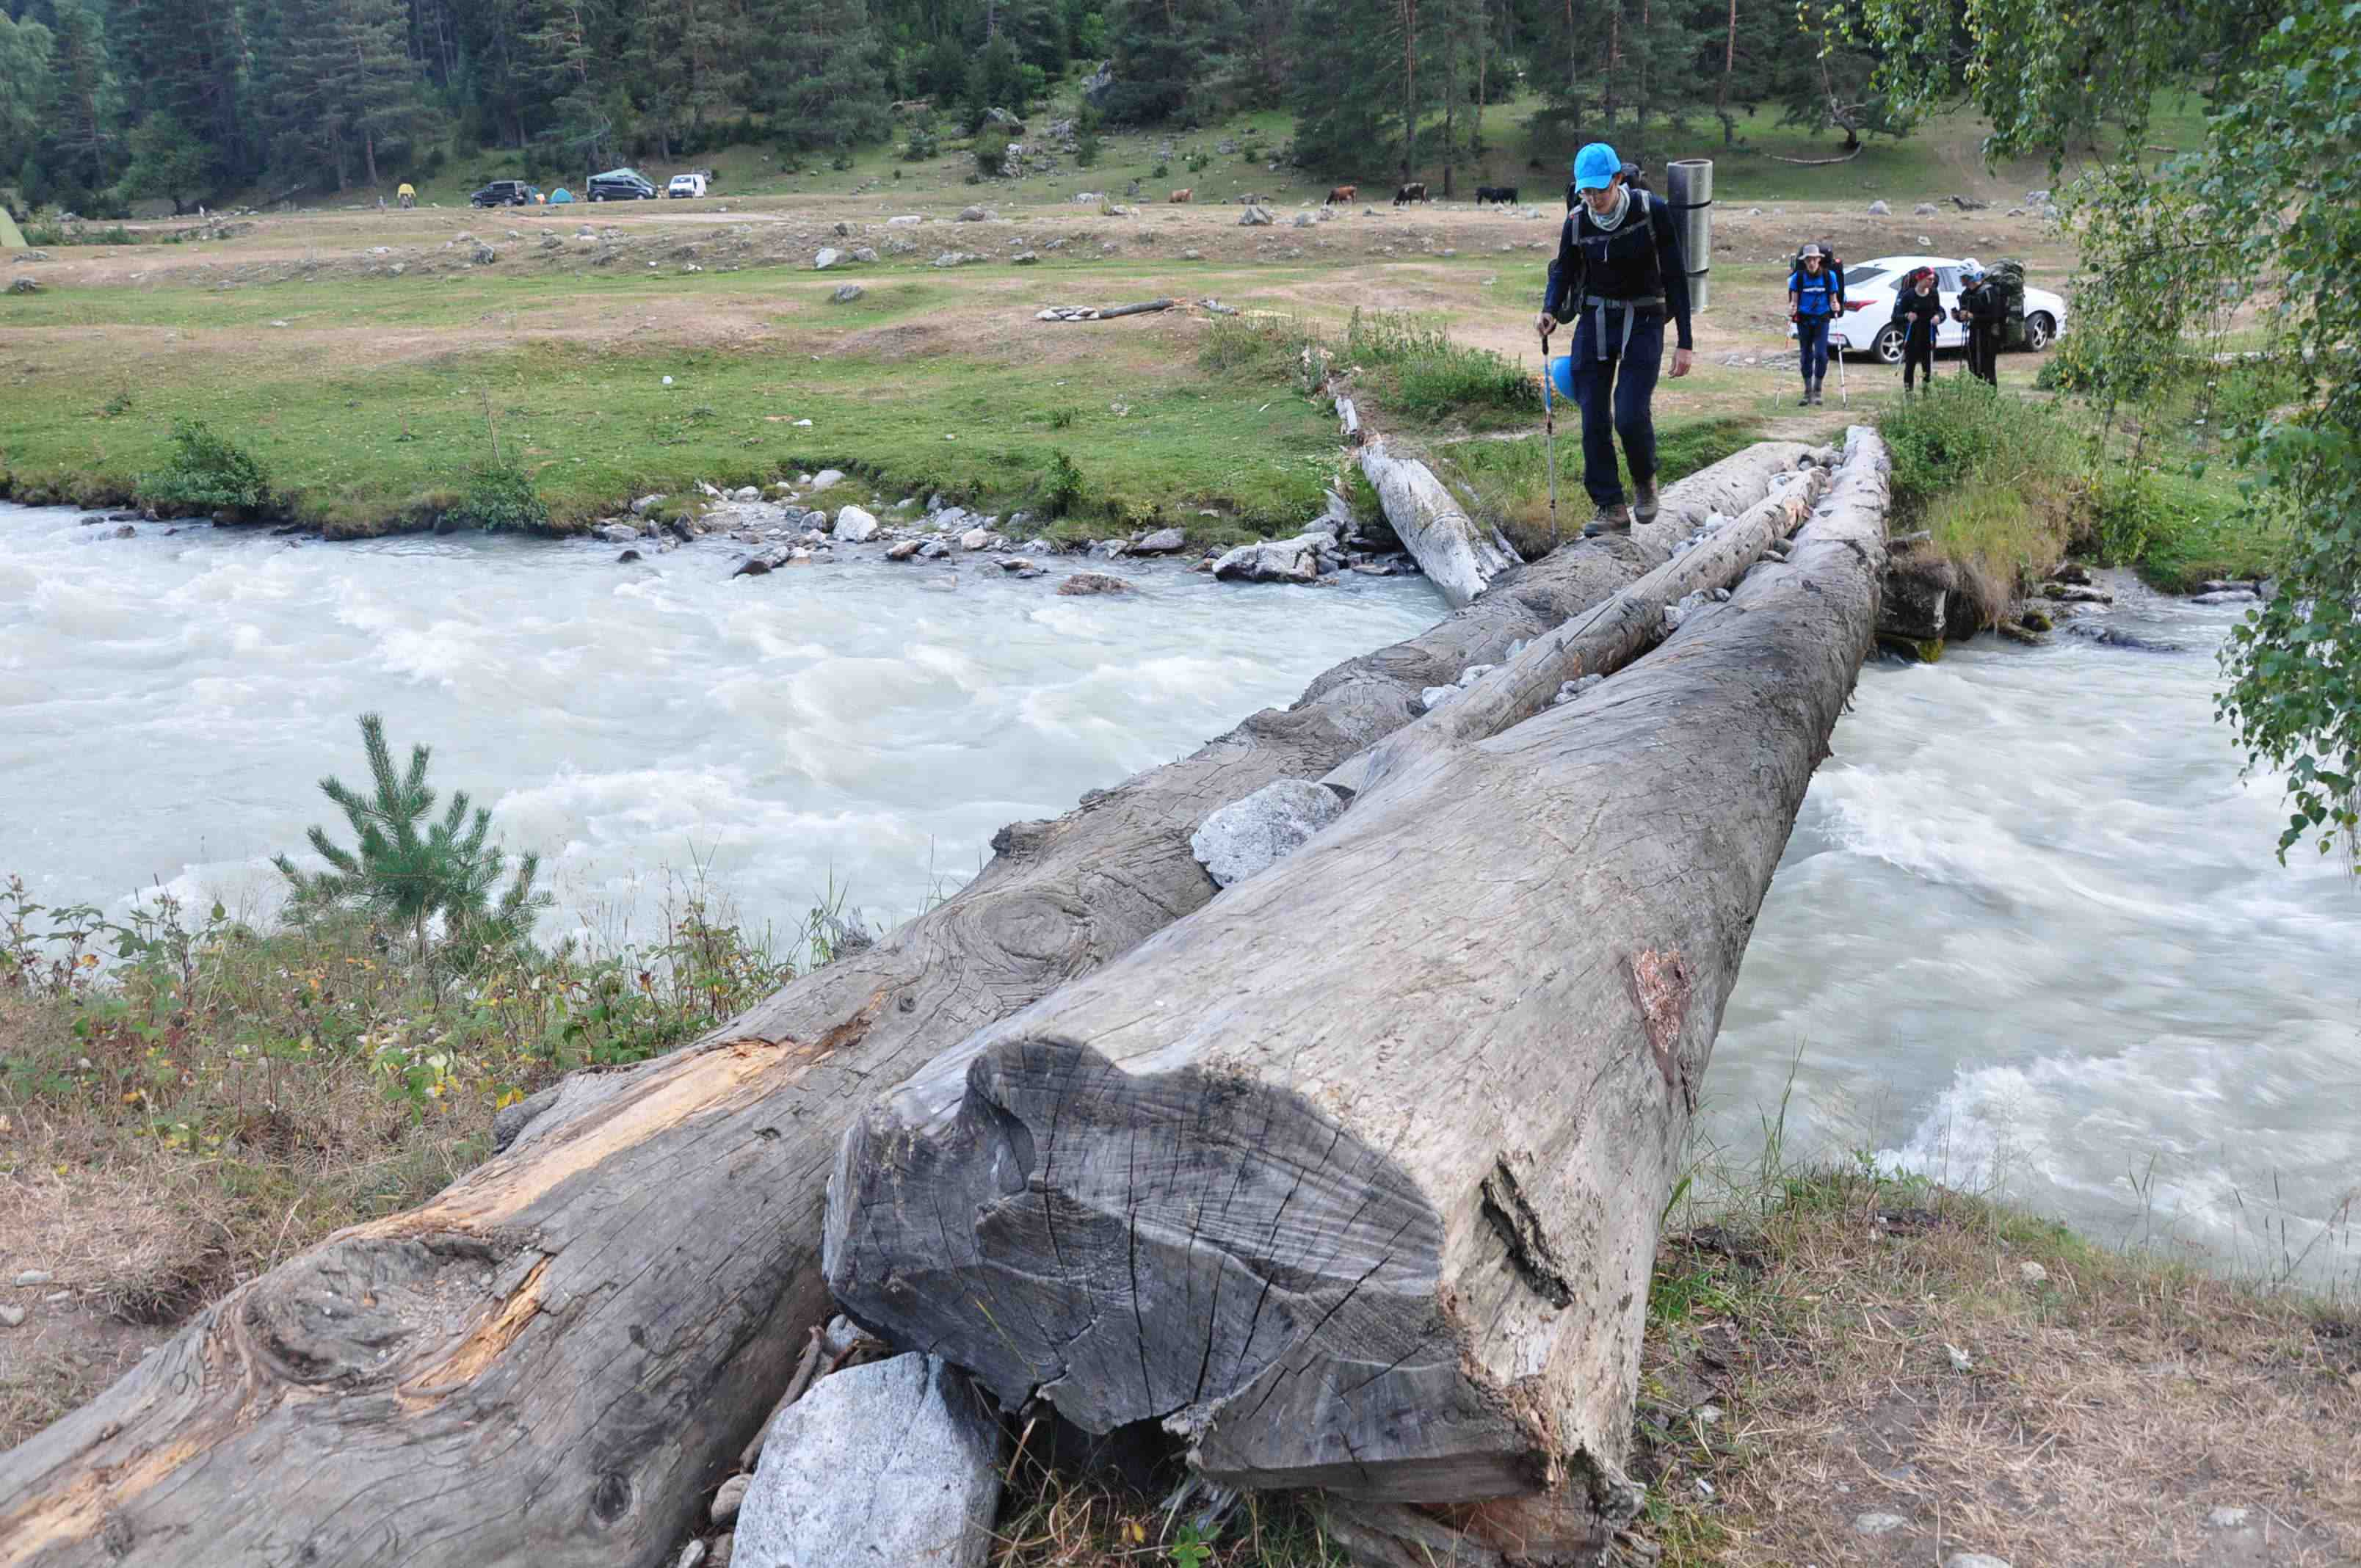
\includegraphics[width=0.7\linewidth]{../pics/DSC_1167}
	\caption{Группа пересекает р. Гондарай по мосту из бревён}
	\label{fig:hondaray}
\end{figure}

На левом берегу реки есть места для ночёвок, но мы приняли решение подняться в по лесной дороге в д.р. Джалпаккол, поскольку руководитель утверждал, что в 2018 году \cite{Korolyov2018} их группа, так же начав подниматься, в итоге развернулась, а на следующий день оказалось, что до конца подъёма не дошли совсем немного. Воспоминание оказалось ошибочным, и мы не рекомендуем последующим группам так делать. Подъём по достаточно крутой лесной дороге, переходящей в тропу, занял около двух с половиной часов, из которых 2 часа ЧХВ было в тёмное время суток с фонариками.

В 20:20 пересекли р. Джалпаккол по мосту, в 21:05 пришли на оборудованные ночёвки у правого притока Джалпаккола. Координаты м.н. N43.303453\degree,~E42.031513\degree. Стоит отметить, что за 200 м до этого места также имеются места для ночёвок, с водой, но менее сухие и удобные (координаты N43.304245\degree, E42.029190\degree).



\clearpage
\subsection{22 августа. Д.р. Джалпаккол}
\newpage
\subsection{23 августа.  Пер. Джалпаккол Северный (1А)}
\textit{Метеоусловия: утром: ясно, тепло, потом??????????}

\begin{figure}[h!]
	\centering
	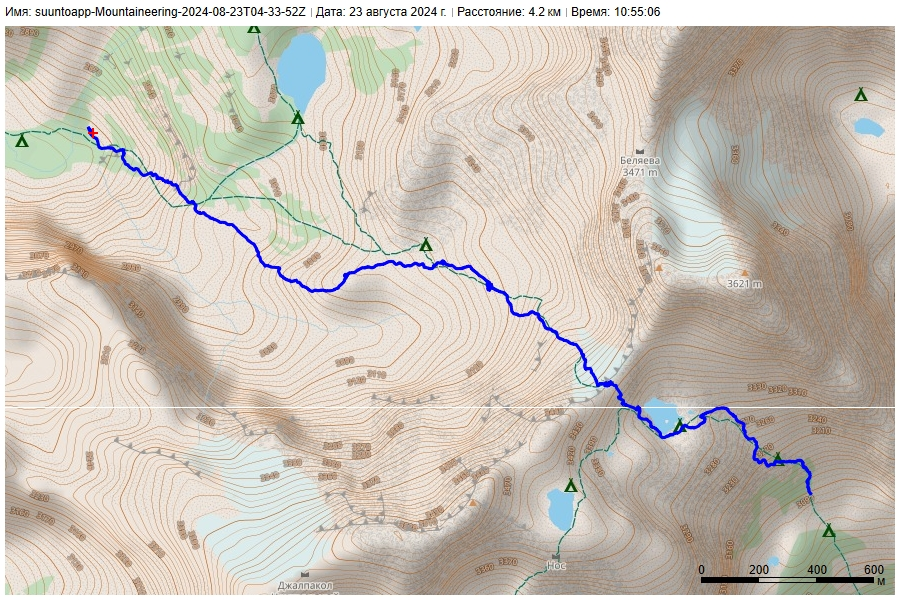
\includegraphics[angle=0, width=0.7\linewidth]{../pics/mini_maps/23}
	\label{fig:mini_23}
\end{figure}


Подъём в 04:30, выход в 07:30. С места ночёвки идёт подъем на моренный вал по помеченной турами тропе (рис.~\ref{fig:23augstart}). В 08:50 оказываемся на развилке троп (левая пхд тропа ведёт на каскадные озёра). Встречаем семейную пару туристов, которые спускались с перевала через эти озера. На развилке делаем привал, на котором Наташа заклеивает колено тейп-лентой и надевает наколенник.

\begin{figure}[h!]
	\centering
	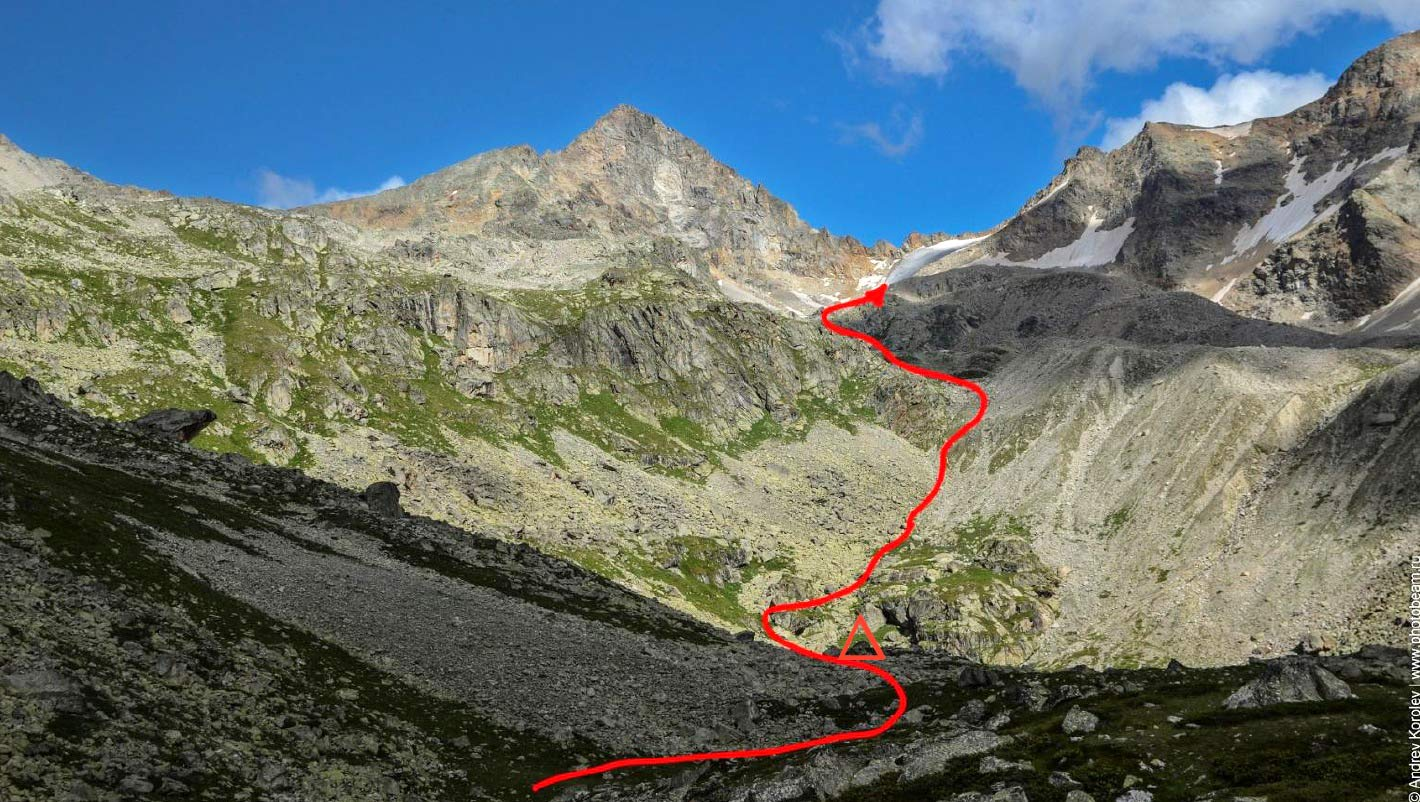
\includegraphics[angle=0, width=0.7\linewidth]{../pics/23augstart}
	\caption{Путь подъёма к перевалу Джалпаккол Северный от места ночёвки. Фото из отчёта Королёва А.Э. \cite{Korolyov2018}}
	\label{fig:23augstart}
\end{figure}

 Далее путь проходит по гребню моренного вала по слабомаркированной турами тропе. В 13:16 подходим под перевальный взлёт. Снега практически нет, ледник полностью открыт (рис.~\ref{fig:dzh_1}). Принимаем решение двигаться по правому пхд борту ледника. Как оказалось позднее, стандартный путь на этот перевал в виде <<крюка>> проходит ещё правее, но в нашем случае, когда снега на перевале не было, он проходил бы по осыпи, что только затруднило бы движение.
 



\begin{figure}[h!]
	\centering
	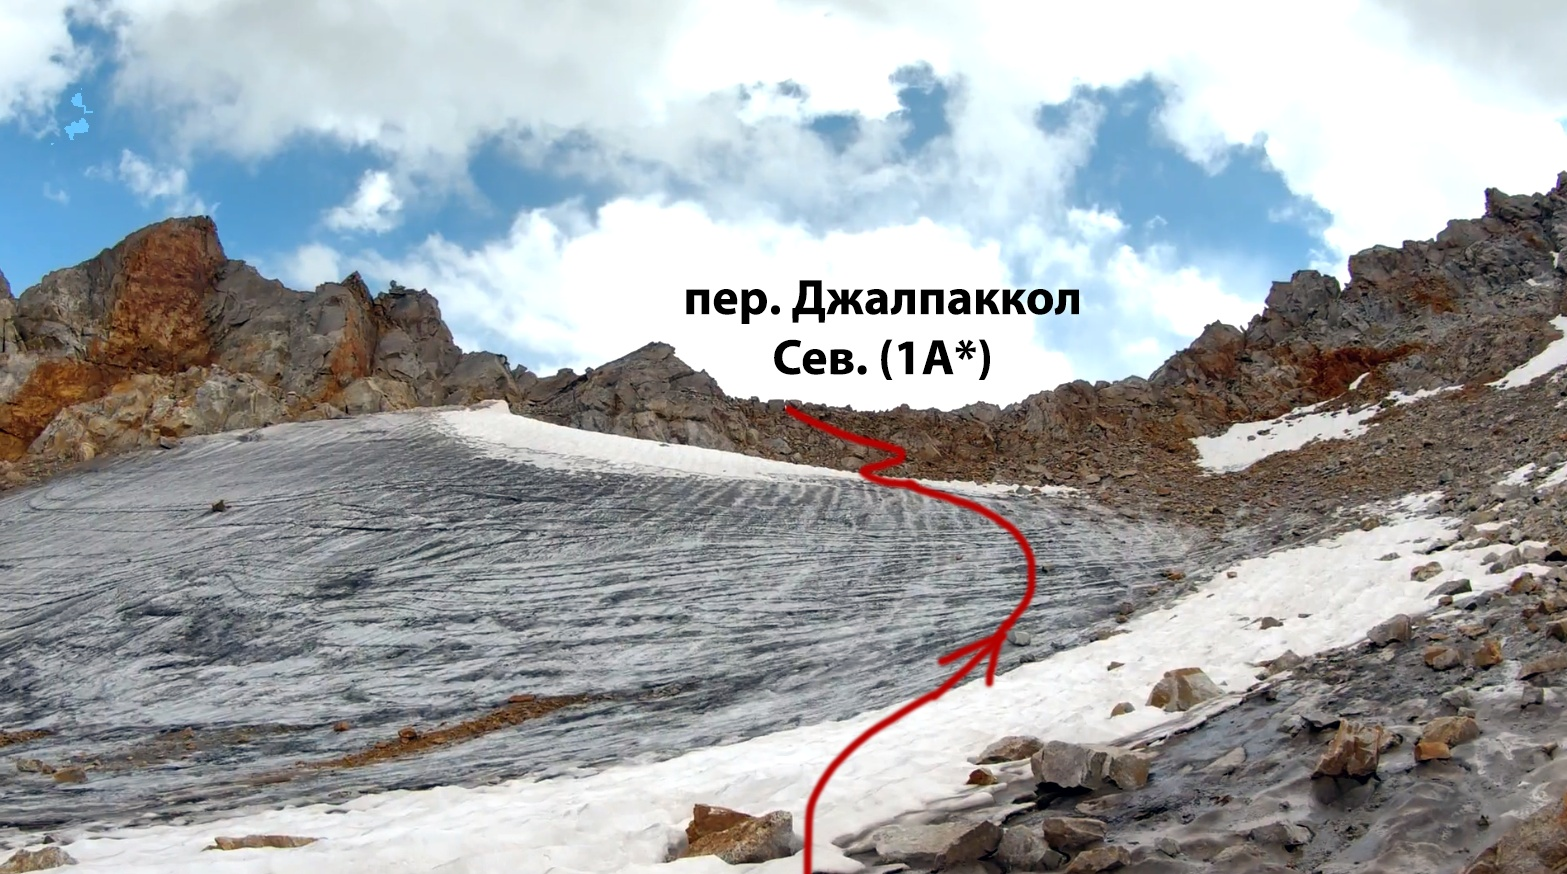
\includegraphics[width=0.7\linewidth]{../pics/dzh_1}
	\caption{Перевальный взлёт пер. Джалпаккол Северный}
	\label{fig:dzh_1}
\end{figure}

\begin{figure}[h!]	
	\centering
	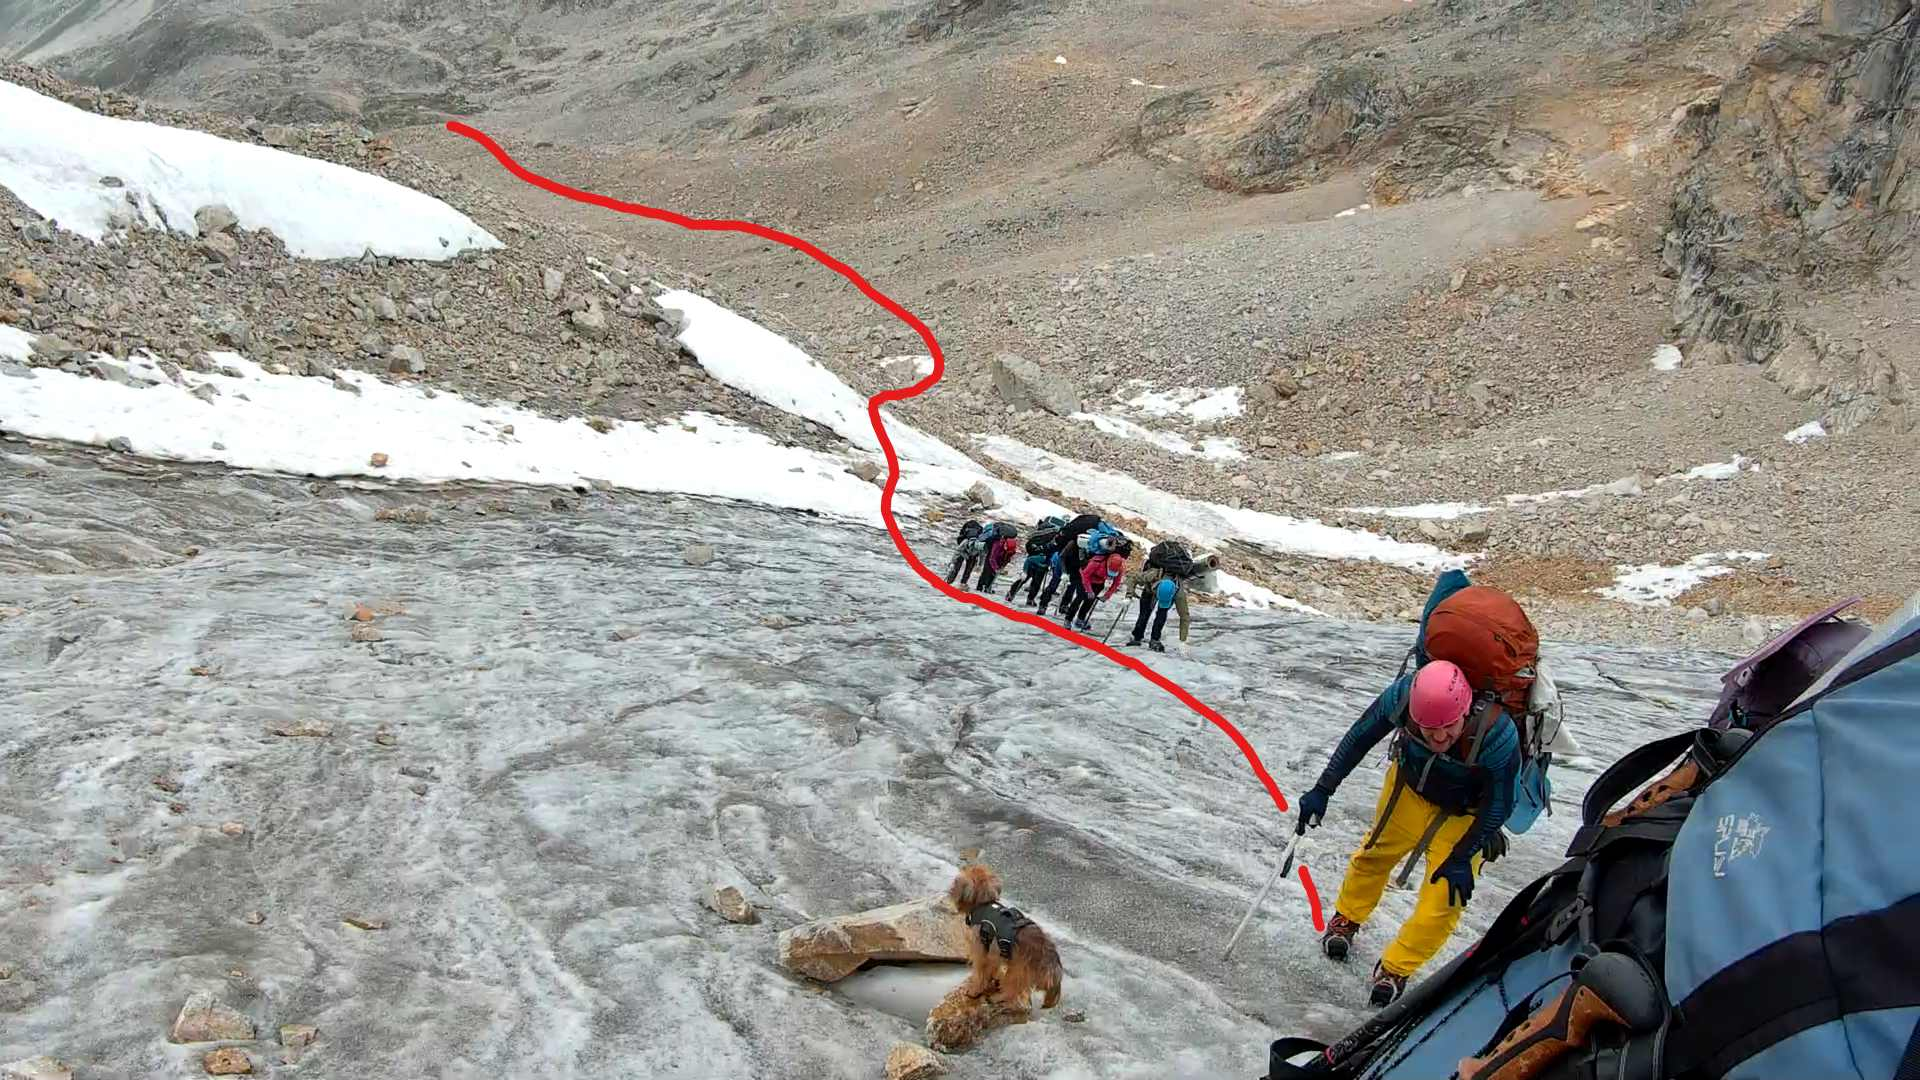
\includegraphics[angle=0, width=0.7\linewidth]{../pics/gopro_dzh}
	\caption{Подъём по леднику}
	\label{fig:gopro_dzh}
\end{figure}

\begin{figure}[h!]	
	\centering
	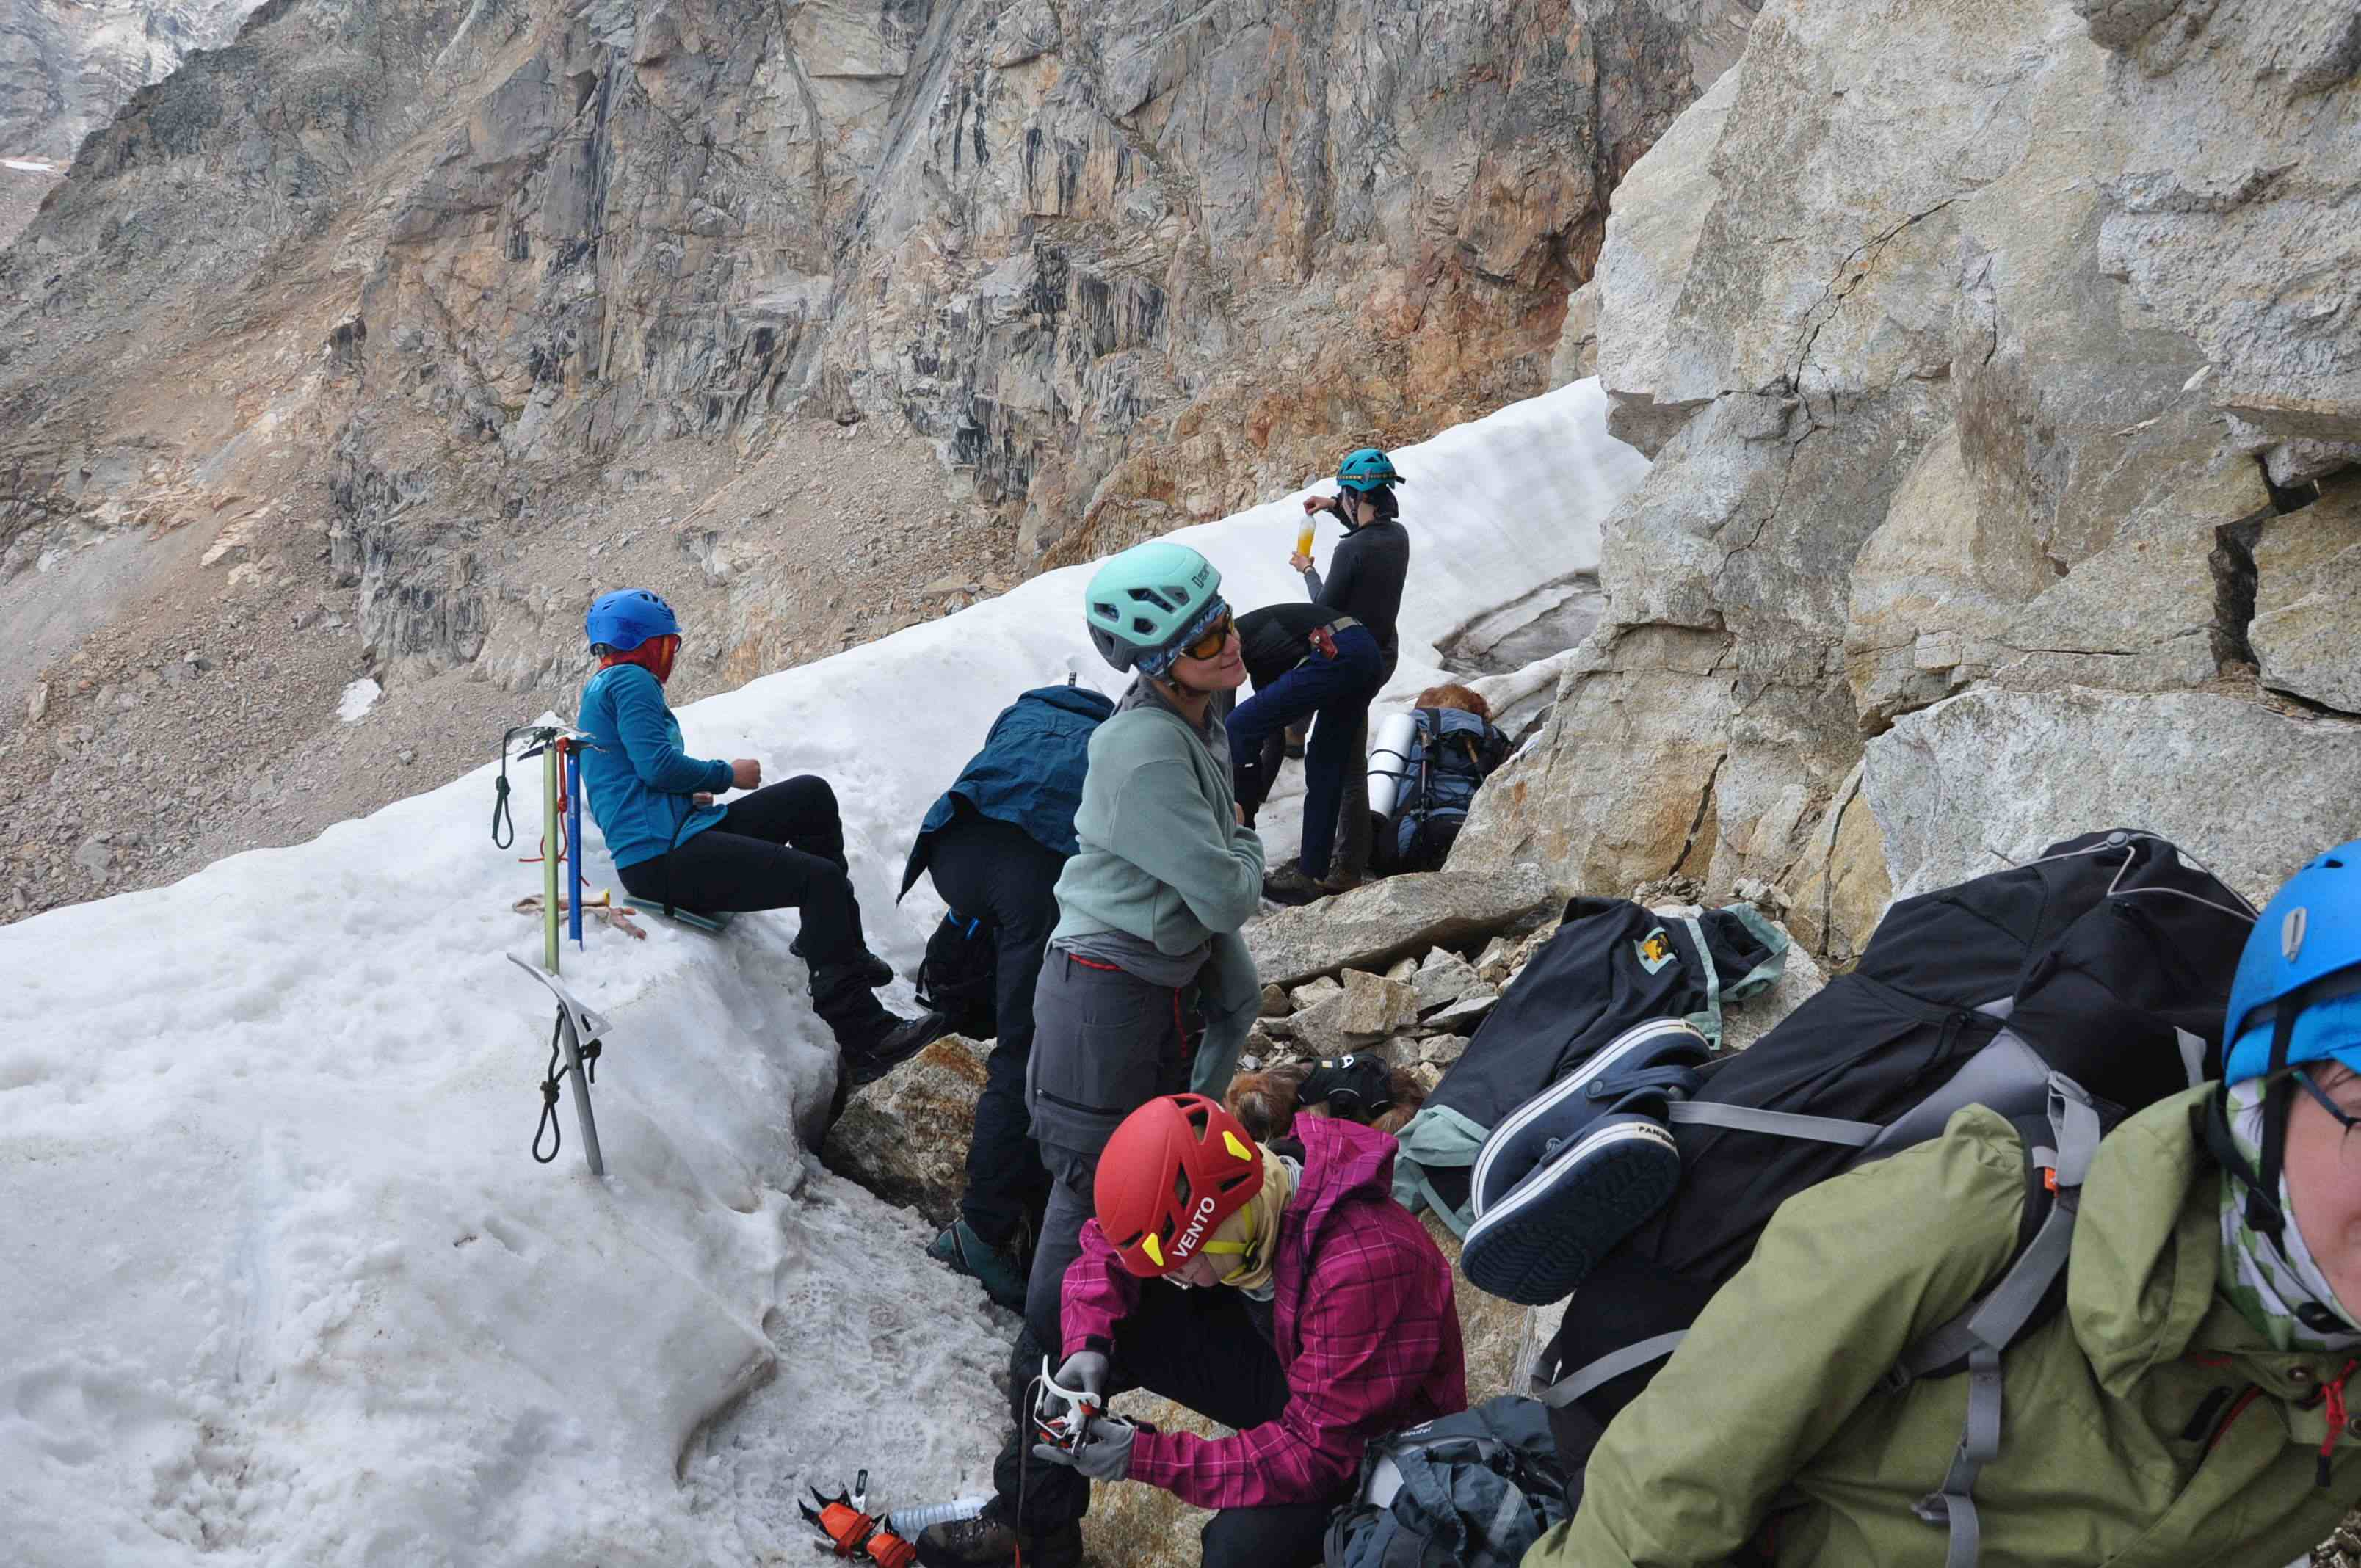
\includegraphics[angle=0, width=0.7\linewidth]{../pics/DSC_0021}
	\caption{Группа перед скальным участком перевала}
	\label{fig:DSC_0021}
\end{figure}


Подъём по леднику занимает 20 минут (рис.~\ref{fig:gopro_dzh}), в 14:45 приходим под финальный участок перевала~--- 10 метров лазания по сильно разрушенным скалам (рис.~\ref{fig:DSC_0021}) и снимаем кошки.




 Погода была хорошая, тепло и солнечно. Основная часть подъёма проходит по курумнику, группа останавливается на привалы каждые 15 минут, привалы длятся 10 минут. В 13:17 группа доходит до ледника и останавливается на технический привал, чтобы надеть кошки и забинтовать ногу Наташе (у нее болело колено). В 14:28 вся группа закончила прохождение ледника, устроили привал, чтобы снять кошки.        

Далее нужно было залезть на скальный гребень (высота где-то 10 м). Сначала руководители забрались без рюкзаков, чтобы определить наиболее удобный и безопасный маршрут, затем участники залезали парами. В 15:08 все взошли на перевал. С перевала открывался вид на озеро и долину реки Мырды.











\newpage
\subsection{24 августа. А/л <<Узункол>>}
\textit{Метеоусловия: утром пасмурно, днём дождь, вечером переменная облачность.}


\begin{figure}[h!]
	\centering
	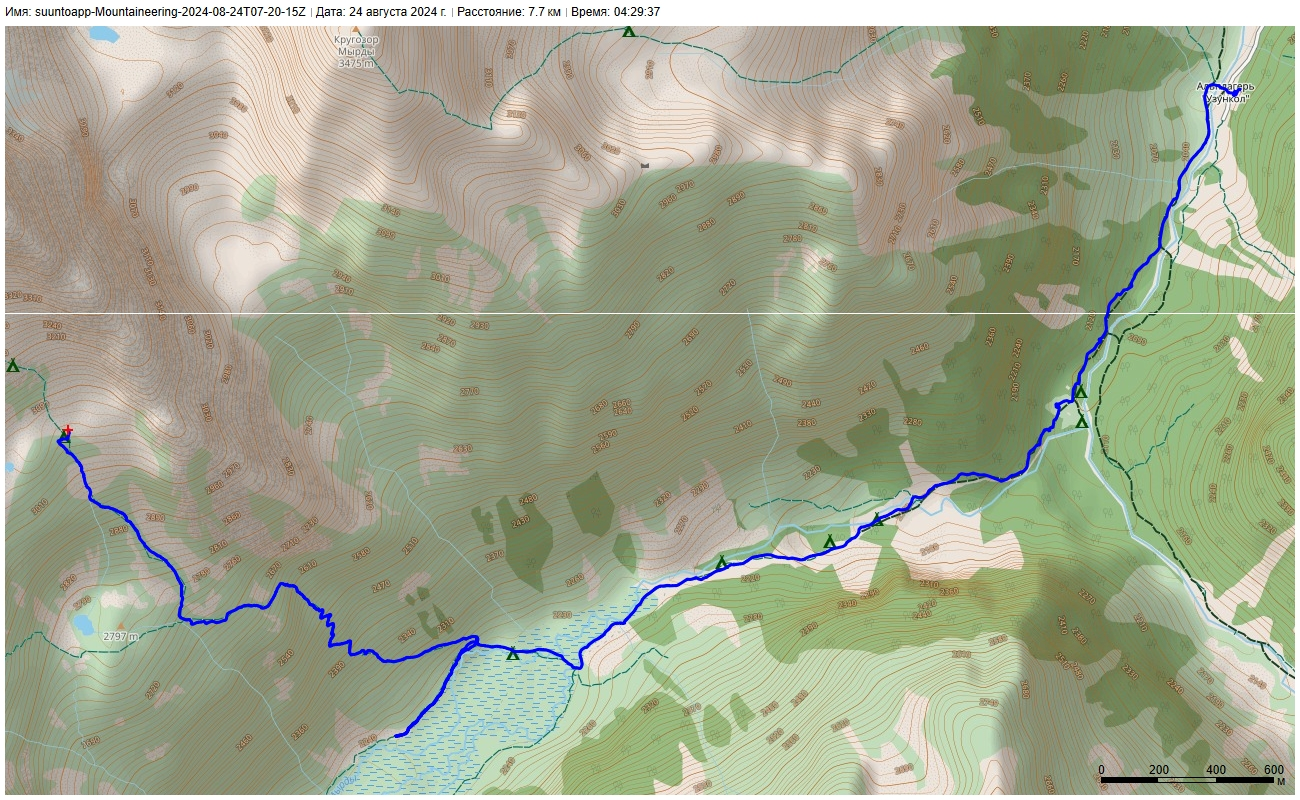
\includegraphics[angle=0, width=0.7\linewidth]{../pics/mini_maps/24}
	\label{fig:mini_24}
\end{figure}



Подъём в 08:00, выход в 10:20. Сегодняшняя наша цель~--- спуститься в а/л <<Узункол>> и устроить там полуднёвку.

Спускаемся по хорошо  набитой тропе, спуск трудностей (помимо зарослей малины и чабреца) не вызывает.
\begin{figure}[h!]
	\centering
	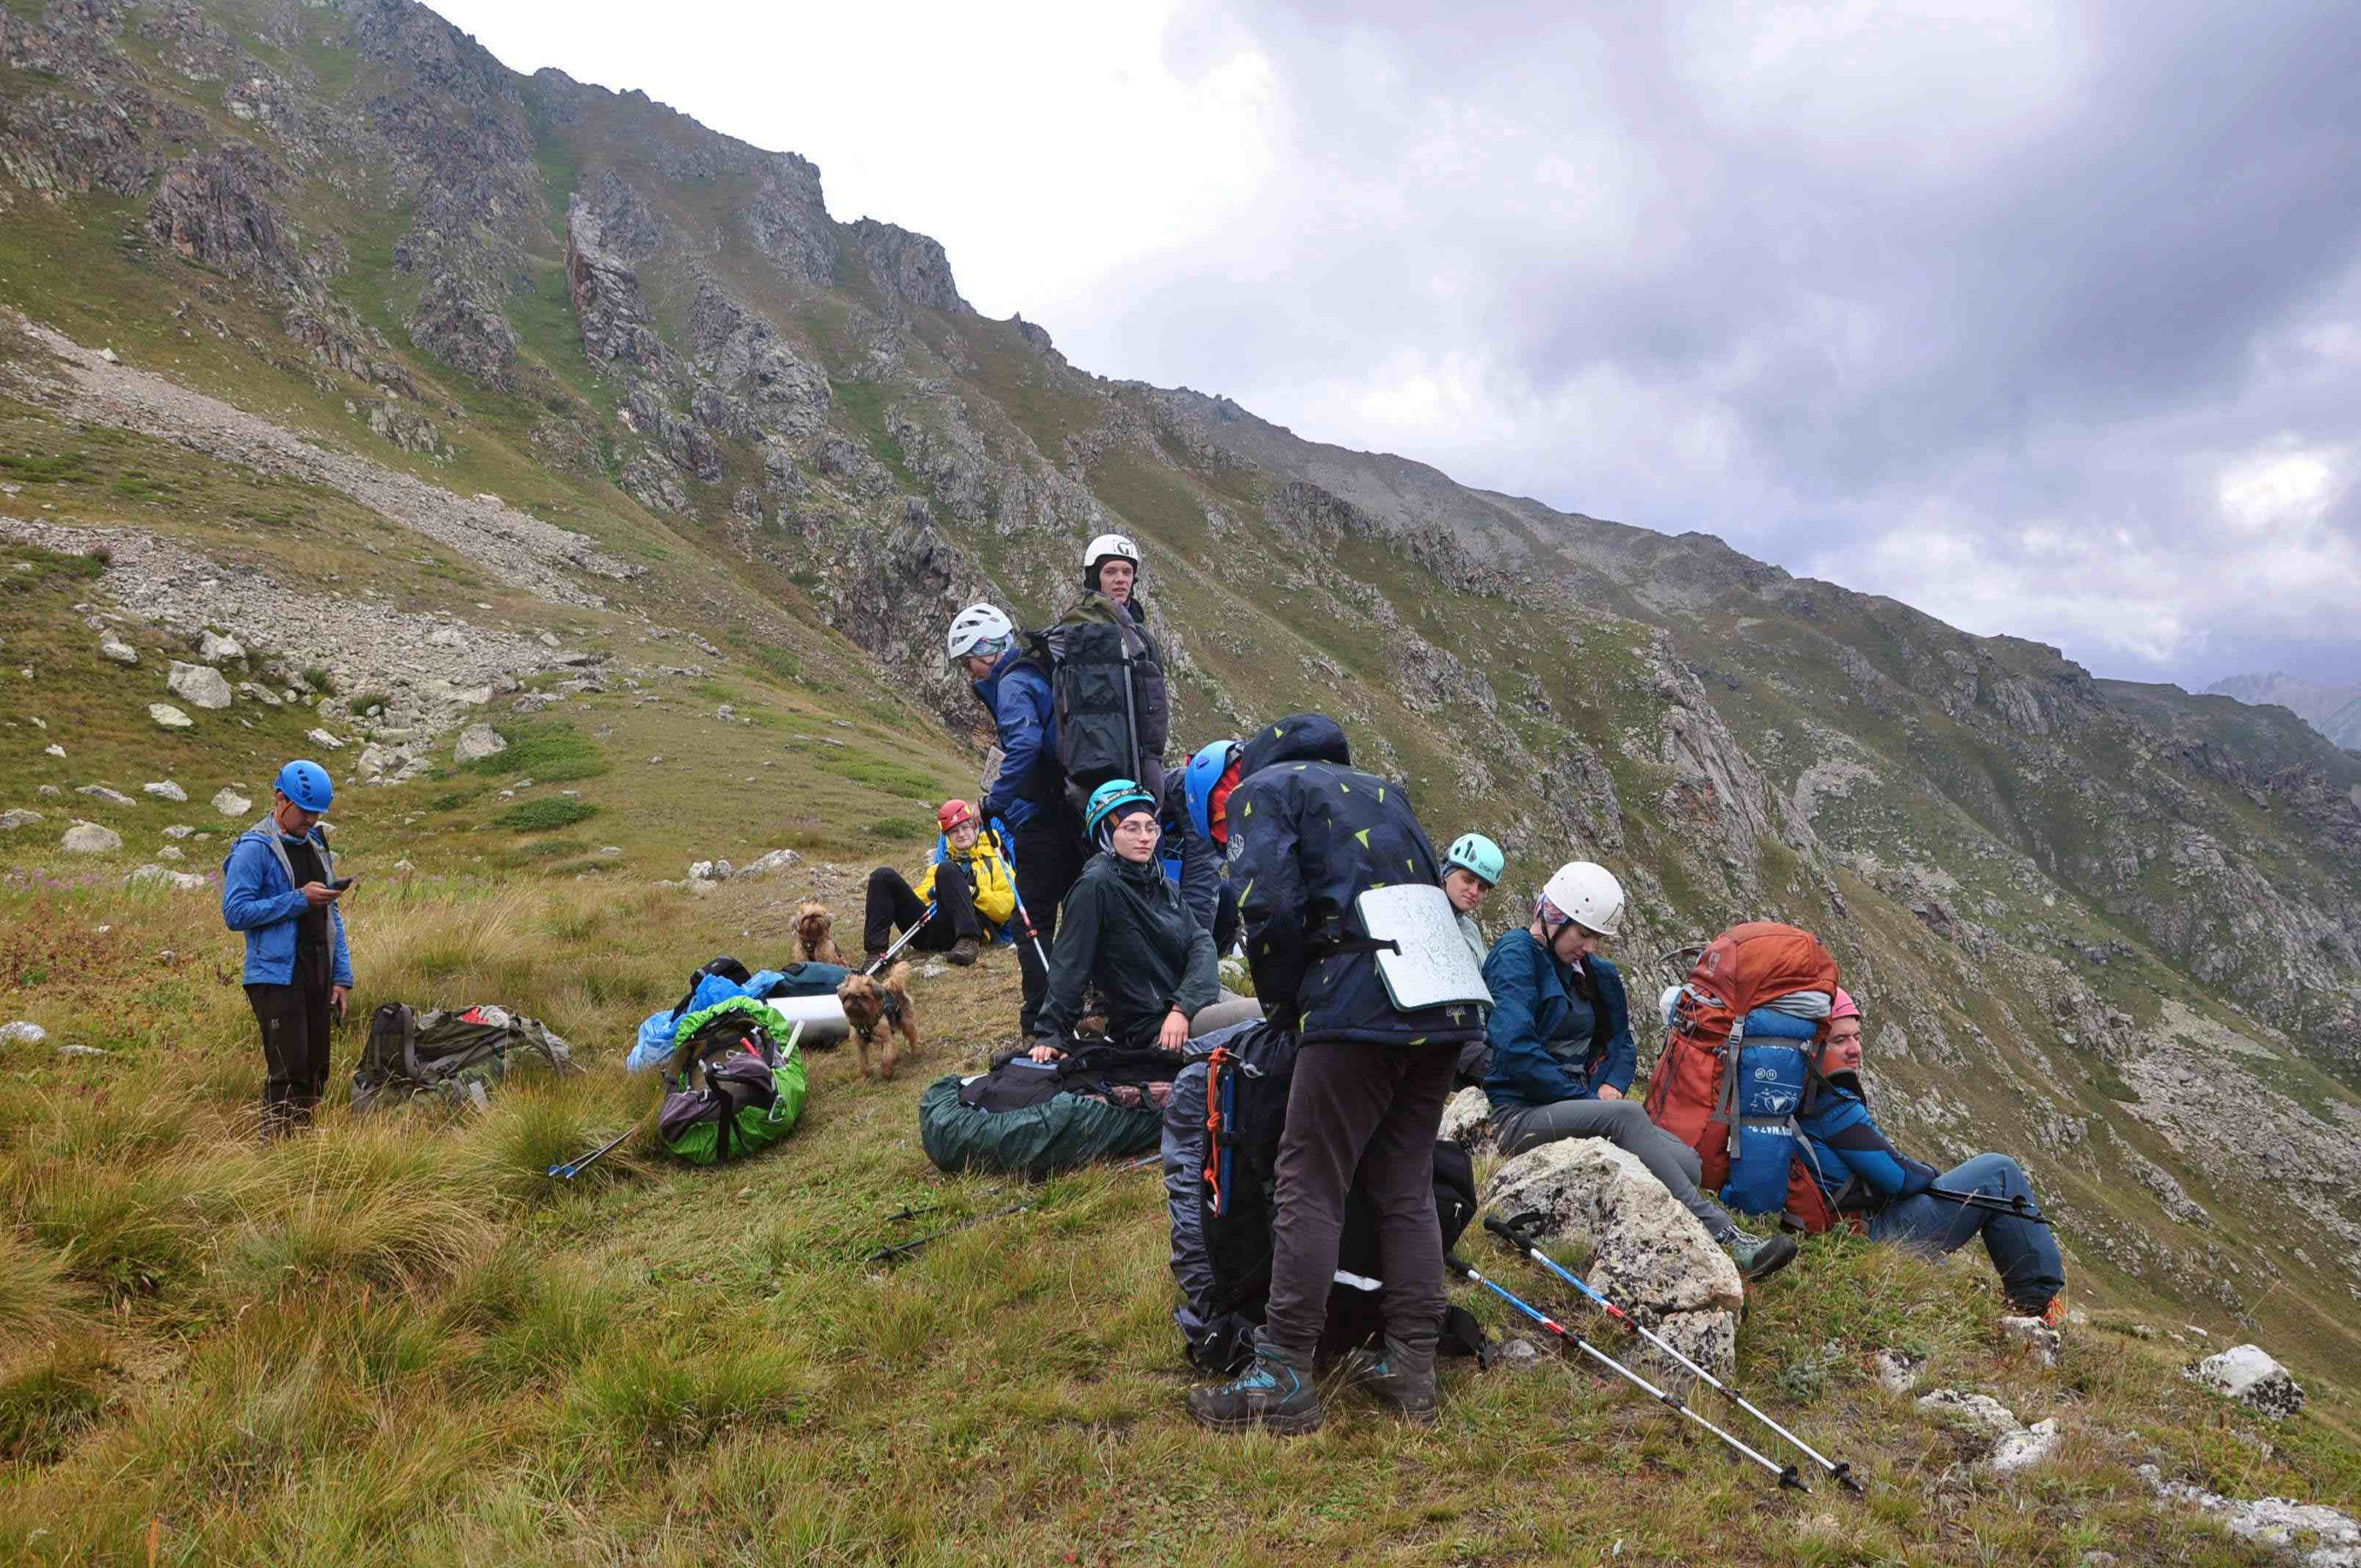
\includegraphics[width=0.7\linewidth]{../pics/DSC_0104.jpg}
	\caption{Группа на спуске в д.р. Мырды}
	\label{fig:DSC_0104.jpg}
\end{figure}

\begin{figure}[h!]
	\centering
	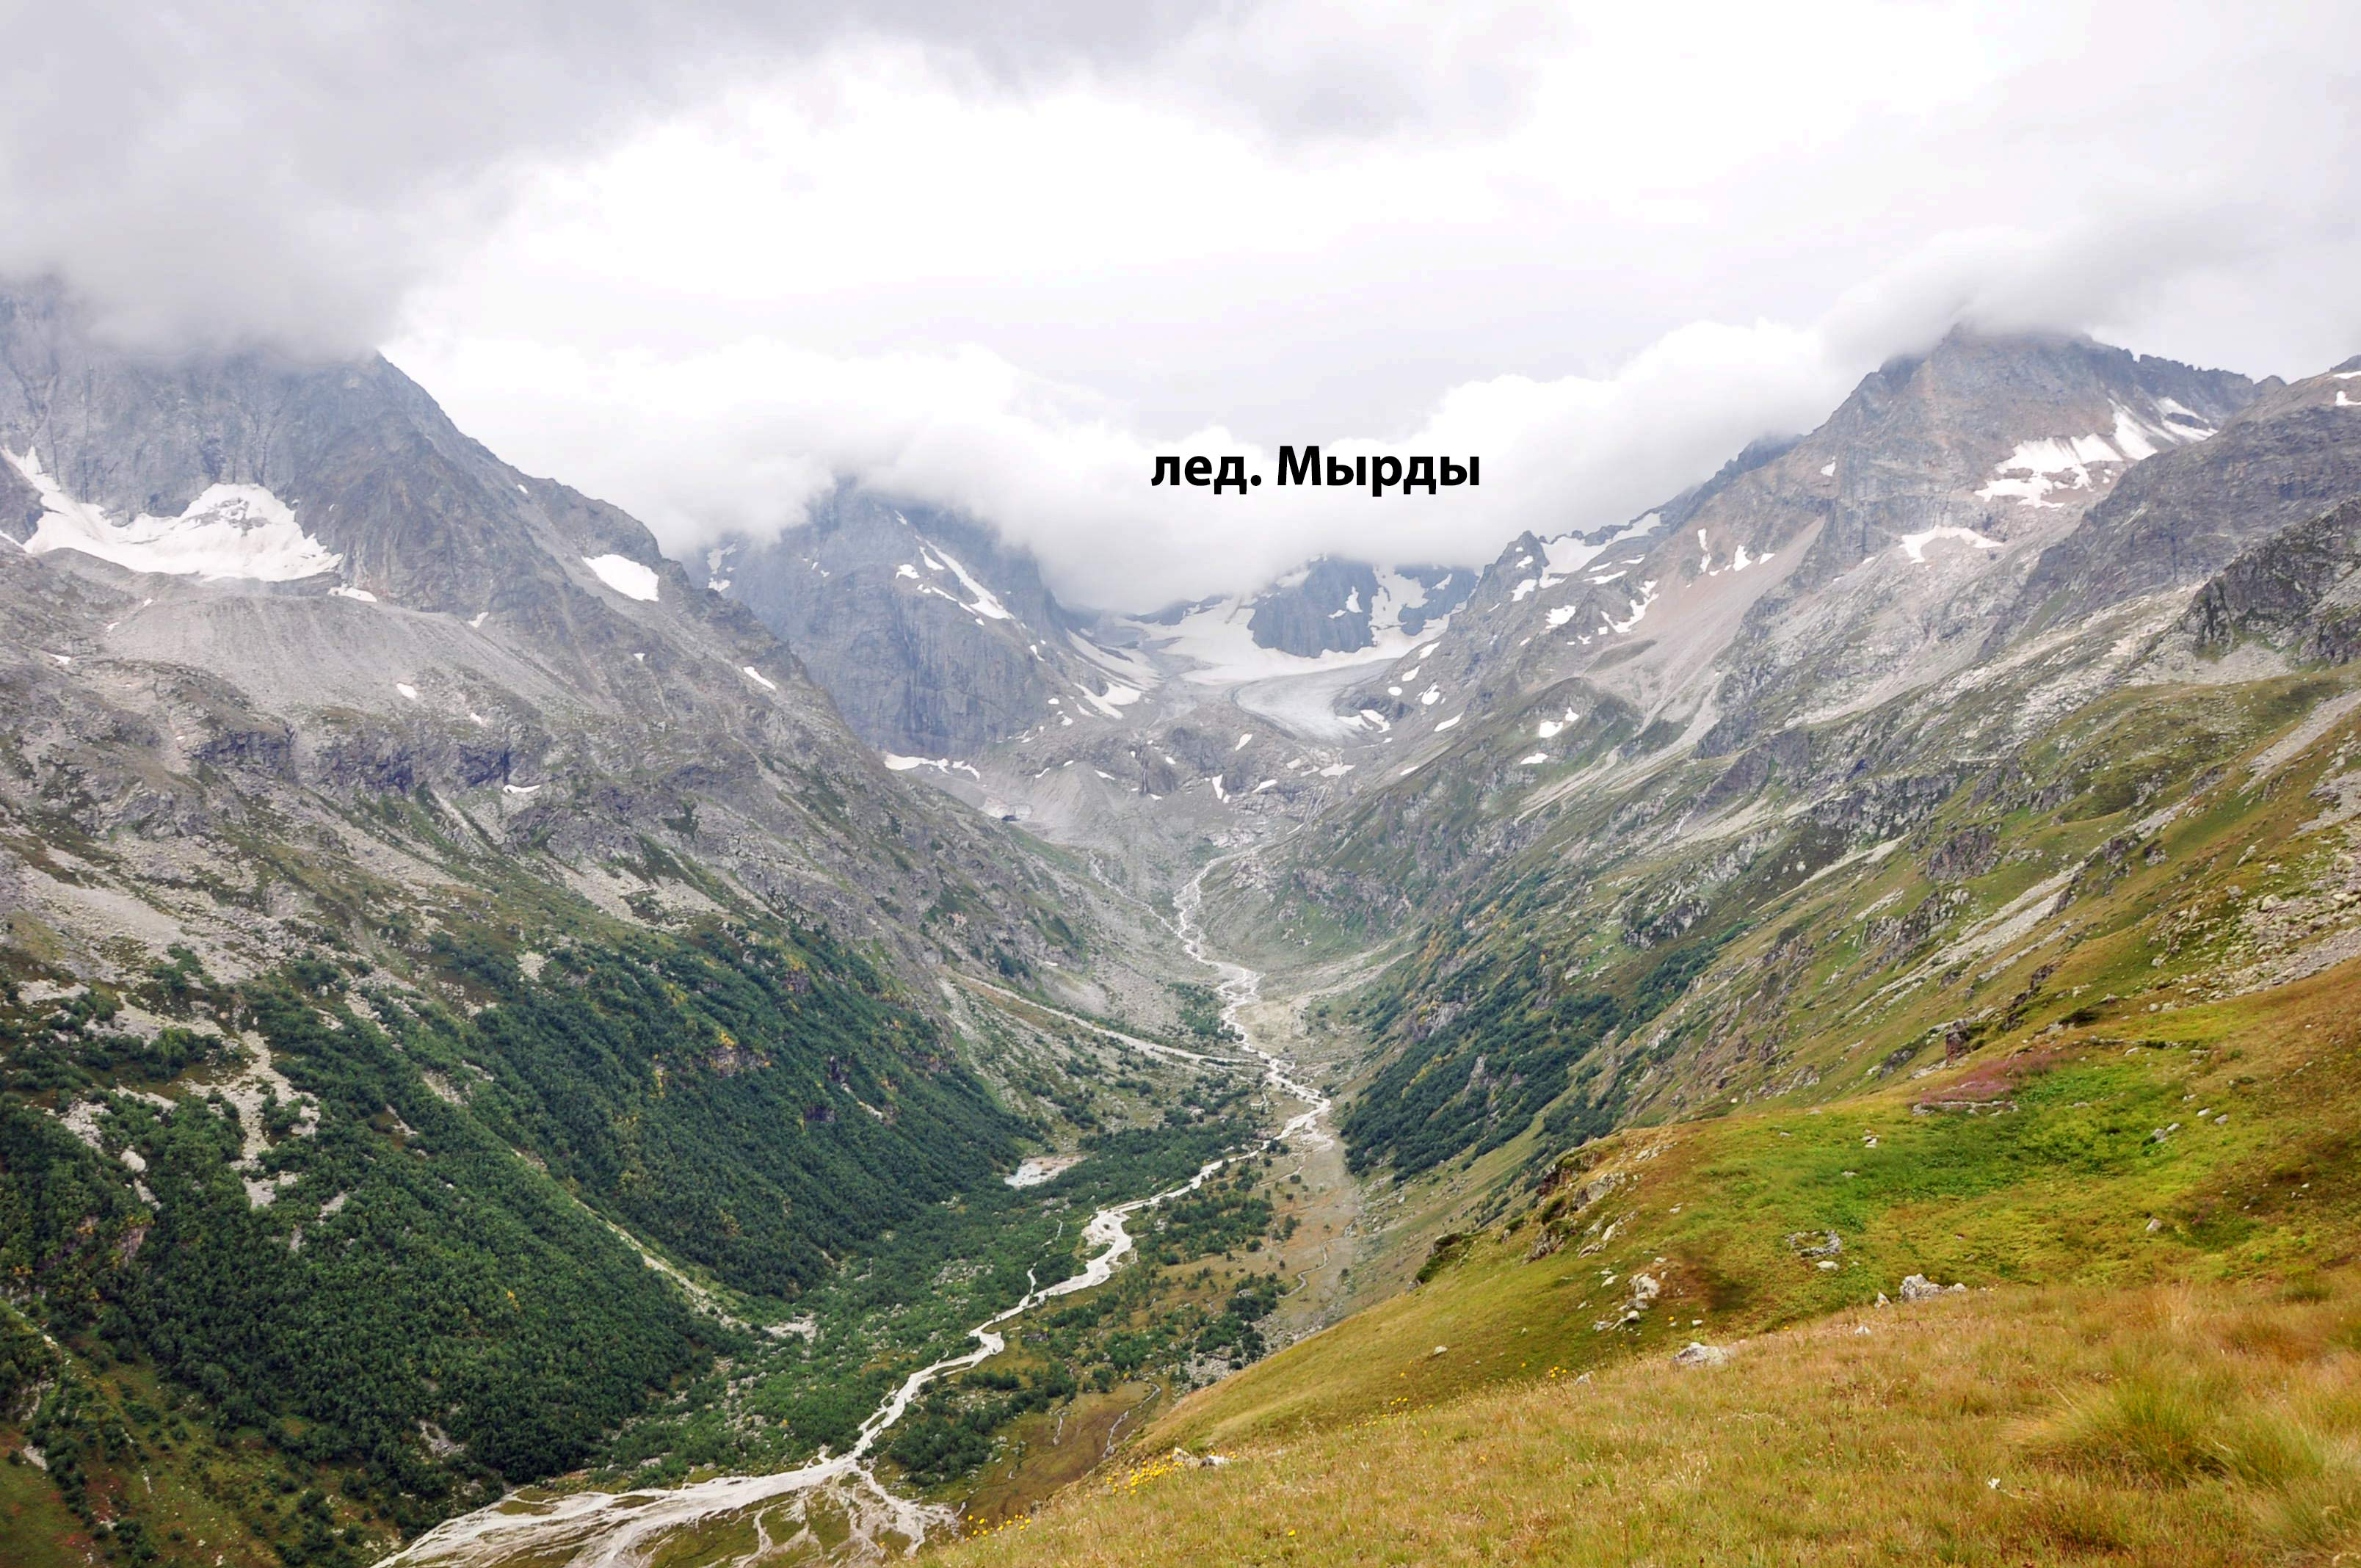
\includegraphics[width=0.7\linewidth]{../pics/DSC_0107.jpg}
	\caption{Верховья р. Мырды}
	\label{fig:DSC_0107.jpg}
\end{figure}

Спустились на дно долины в 12:50. Попутно нас обгоняли многочисленные группы гуляющих налегке туристов из а/л <<Узункол>>.

Спустившись к реке, устроили привал, в ходе которого часть группы прошла 400 м вверх по течению в поисках <<нарзанных источников>> N~43.264012\degree, E~42.137496\degree~(рис. \ref{fig:DSC_0111.JPG}). Фактически, мы нашли несколько источников воды, богатой железом и с сильным запахом сероводорода: по вкусовым ощущениям эта вода не шла ни в какое сравнение с нарзанными источниками в д.р. Махар около т/б <<Глобус>>.

\begin{figure}[h!]
	\centering
	\includegraphics[width=0.7\linewidth]{../pics/DSC_0111.JPG}
	\caption{Группа в поисках нарзанных источников}
	\label{fig:DSC_0111.JPG}
\end{figure}

Далее переходим р. Мырды по хорошему пешеходному мосту на правый берег и идём по автомобильной дороге. Разрушенный мост через р. Мырды, ведущий на левый берег и упоминавшийся в отчёте \cite{Korolyov2018} как разрушенный, в настоящий момент восстановлен, его координаты N~43.271433\degree, E~42.159714\degree. Рядом находится автомобильный брод.

В 14:20 подходим к погранзаставе. Проверка документов занимает менее 10 минут, после чего идём к альплагерю, где оказываемся в 14:45.

Народу в альплагере много, но места под палатки есть. С нас берут 500~\faRub~с человека за ночь. В стоимость, помимо места под палатку, входит горячий душ, возможность подзарядить гаджеты и воспользоваться интернетом (последнее~--- с 19:00 по 23:00). За хранение заброски с нас взяли 100~\faRub~за мешок в день. Вечером мы воспользовались баней (2500~\faRub~с группы за час). Остаток дня потратили на отдых, стирку, распределение заброски и празднование годовщины свадьбы руководителя и зам. руководителя.



\newpage
\subsection{25 августа. Д.р. Кичкинекол}
\newpage
\subsection{26 августа. Пер. Кичкинекол Малый (1А)}
\textit{Метеоусловия: утром переменная облачность, днём, вечером сильный дождь, ветер.}

\begin{figure}[h!]
	\centering
	\includegraphics[angle=0, width=0.7\linewidth]{../pics/mini_maps/26}
	\label{fig:mini_26}
\end{figure}

Подъём в 08:00. Ночная гроза закончилась, небо было затянуто облаками, периодически проглядывало солнце, что позволило немного подсушить палатки и спальники. Вышли в 11:00, на тропу, траверсирующей травянистый склон. Эта тропа обходит водопад на западной оконечности поляны слева пхд. Встречаются туры, тропу видно хорошо. 
Постепенно травянистый склон переходит в морену.

\begin{figure}[h!]
	\centering
	\includegraphics[width=0.7\linewidth]{../pics/DSC_0221.JPG}
	\caption{Путь подъёма на перевал}
	\label{fig:DSC_0221}
\end{figure}
 
За поворотом нам открылся вид на наш перевал и цирк соседнего перевала Обманный (рис.~\ref{fig:DSC_0226}).
 
\begin{figure}[h!]
	\centering
	\includegraphics[width=0.7\linewidth]{../pics/DSC_0226}
	\caption{Маршрут движения группы}
	\label{fig:DSC_0226}
\end{figure}

Погода тем временем ухудшилась, начался небольшой дождь.

Подъём на перевал проходит по средней и мелкой осыпи; группа шла косыми траверсами с самостраховкой треккинговыми палками. Технической сложности подъём на Кичкинекол Малый не представляет.
В 13:15 вышли на седловину перевала (рис.~\ref{fig:DSC_0239}). Погода испортилась вконец, пошёл косой ливень с градом. Сняли перевальную записку т/к <<Крокус>> (г.~Краснодар) от 24.08.2024~г.; нашу записку руководитель писал на каске участника, пока остальная группа укрывала их обоих полами дождевика-пончо. Кое-как запихнули в себя перевальный шоколад и в 13:22 начали спуск.


\begin{figure}[h!]
	\centering
	\begin{minipage}[h]{0.48\linewidth}
		\includegraphics[width=0.99\linewidth]{../pics/DSC_0239.jpg}
	\end{minipage}
	\quad
	\begin{minipage}[h]{0.48\linewidth}
		\includegraphics[width=0.99\linewidth]{../pics/DSC_0242.jpg}
	\end{minipage}
	\caption{Группа на пер. Кичкинекол Малый. Слева: вид в д.р. Чунгур-Джар, справа: вид в д.р. Таллычат}
	\label{fig:DSC_0239}
\end{figure}

Спуск с перевала идёт также по хорошо набитой тропе травянисто-осыпного склона; периодически встречаются туры. Справа от тропы нам открывался живописный вид на ГКХ, ледник Чунгур-Джар. Ливень тем временем превратился в мелкий дождь. В 15:00 спустились на урочище Аэродром в д.р Чунгур-Джар. Рельеф в этом месте представляет из себя бугристый конгломерат, поэтому поиск места для ночёвки представлял отдельную задачу. По воспоминаниям руководителя, их группа \cite{Korolyov2018} ночевала на правом берегу р. Чунгур-Джар, --- но это было при том, что группа отказалась от сквозного прохождения Перемётного, и могла позволить себе встать ниже по долине. То место ночёвки хорошо просматривалось, но для него требовалось перебродить реку, и, главное, довольно сильно спуститься, --- при том, что у нас ещё оставалась вероятность идти на следующий день на Перемётный. На левом же берегу были огороженные камнями места под палатки, которые, впрочем, не выглядели так чтобы очень уютно. Провели разведку с бродом: разведка показала, что на данном уровне на противоположном берегу палатку поставить точно нельзя, --- поэтому остановились на варианте с огороженными <<не очень уютными>> площадками. Дождь всё это время не прекращался, сопровождаясь сильным ветром.

Обед приготовили участники-<<волонтёры>>, которые чувствовали себя более-менее неплохо, --- остальные сушились и грелись в палатках. Координаты м.н.: N43.248385\degree,~E42.236151\degree.

\begin{table}[h!]
	\centering
	\begin{tabular}{|c|c|c|c|c|c|} 
		\hline 
		Этап & ЧХВ \\ 	
		\hline 
		От а/л <<Узункол>> до начала косого траверса  & 01:05 \\
		Подъём косым траверсом из д.р. Кичкинекол до нижних ночёвок  & 01:18 \\
		Подъём к Поляне Крокусов & 01:00\\ 
		Подъём на седловину перевала & 02:08\\ 
		Спуск с седловины до урочища <<Аєродром>> & 01:07 \\
		
		\hline
		\textsc{Полное время подъёма на перевал  }& 05:38\\
		\textsc{Полное время спуска с перевала }& 01:07 \\
		\textsc{Полное время прохождения перевала }& 06:45 \\
		\hline
	\end{tabular}
	\caption{Расклад времени, пер. Кичкинекол Малый}
\end{table}

\paragraph{Выводы и рекомендации:} пер. Кичкинекол Малый полностью соответствует своей категории сложности и не является сложным ни технически, ни физически. Рекомендуется к прохождению новичковым группам в качестве первого перевала в походе. Стоит, однако, иметь в виду, что в непогоду тропа на спуск в д.р. Чунгур-Джар может быть скользкой и размытой; требуется спускаться с осторожностью.

\clearpage
\subsection{27 августа. Пер. Перемётный (1А)}
\textit{Метеоусловия: утром, днём, вечером ясно, тепло.}

\begin{figure}[h!]
	\centering
	\includegraphics[angle=0, width=0.7\linewidth]{../pics/mini_maps/27}
	\label{fig:mini_27}
\end{figure}




\begin{figure}[h!]
	\centering
	\includegraphics[width=0.7\linewidth]{../pics/perem_1}
	\caption{Начало подъёма к пер. Перемётный из д.р. Чунгур-Джар}
	\label{fig:perem_1}
\end{figure} 


Метеоусловия: солнечно, тепло

Утром проснулись в 7:00, долго стирались, чинились и сушились, руковод курил какао и размышлял... Переметный было решено брать!
В 10:00 выдвинуль в сторону перевала.

\begin{figure}[h!]
	\centering
	\includegraphics[width=0.7\linewidth]{../pics/DSC_0251.jpg}
	\caption{Утренний лагер. Активно сушимся.}
	\label{fig:DSC_0251}
\end{figure}

\textbf{Задача номер раз:} перейти многорукавье реки Чунгур-Джар. Оказалось сложнее, чем казалось. Часть группы промочила ботинки и усердно их сушила на каждом привале.

\begin{figure}[h!]
	\centering
	\includegraphics[width=0.7\linewidth]{../pics/DSC_0254.jpg}
	\caption{р. Чунгур-Джар. Нам предстоит перебраться через множество ручейков.}
	\label{fig:DSC_0254}
\end{figure}
\begin{figure}[h!]
	\centering
	\includegraphics[width=0.7\linewidth]{../pics/DSC_0277.jpg}
	\caption{р. Чунгур-Джар. Перебрались.}
	\label{fig:DSC_0277}
\end{figure}

\textbf{Задача номер два:} пройти подъем на перевал. Поднялись на морену по травянисто-каменстому склону, прошли по гребню и попрощались на время с травой. На высоте 2410м (N 43.24135, E 42.24827) начали траверс по сыпухе и под небольшой скалой на соседнюю морену.
\begin{figure}[h!]
	\centering
	\includegraphics[width=0.7\linewidth]{../pics/DSC_0280.jpg}
	\caption{Траверс по моренам.}
	\label{fig:DSC_0280}
\end{figure} 
После этого - прямым курсом на перевал. С задачей два справились в 14:38. На перевале сняли записку группы туристов из Ростова-на-Дону и Новочеркасска от 20.08.2019 \ref{pic:peremetnyy}. Примечательно, что эта группа в свое время сняла записку Горной секции МФТИ под руководством Королева Андрея от 2018 года - в этот поход ходила руковод.

\begin{figure}[h!]
	\centering
	\includegraphics[width=0.7\linewidth]{../pics/DSC_0419 2.jpg}
	\caption{Перевал Переметный. Вид на Эльбрус.}
	\label{fig:DSC_0419 2}
\end{figure} 

\textbf{Задача три:} спуститься в низ, в д.р. Танышхан. Здесь начинается очень интересная и поучительная история.
\begin{figure}[h!]
	\centering
	\includegraphics[width=0.7\linewidth]{../pics/perem_down.png}
	\caption{Спуск с перевала переметный.}
	\label{perem_down}
\end{figure} 
Выдвинулись в 15:38. Вниз сначала шли по сыпухе забирая влево, усердно считали моренные валы чтобы не ошибиться и не угодить в березняк. По пути старались расставлять турики, но время подгоняло, в маршруте мы были не  уверены и на полпути мы это дело забросили.  Потом начался травянистый склон, альпеншток альпеншточил на все 100. После спуска на 130 м выбрались на курумник, на котором не обошлось без легкого кровопролития. К сумеркам снова вышли на травянистый склон. Русло пересохшего ручья (N 43.25779° E 42.27107°), засыпанного крупными камнями, предоставило удобный вариант до спуска. К моменту, когда мы добрались до зарослей рододендронов, уже порядком стемнело (19:05), дальше по лощине шли с фонарикам. 

В 20:00 вышли на отличную стоянку на берегу реки Танышхан (N 43.26002, E 42.27489). Поужинали, и легли спать. С задачей три справились!


\clearpage
\subsection{28 августа. Д.р. Чиринкол}

\textit{Метеоусловия: ????.}

\begin{figure}[h!]
	\centering
	\includegraphics[angle=0, width=0.3\linewidth]{../pics/mini_maps/28}
	\label{fig:mini_28}
\end{figure}

*воспоминания вики: проснулись, пошли по кустарникам вдоль реки, вышли к мужикам, гоняющим коровок, вдоль накатанной дороги и по цивильным мостам дошли до места стоянки*

\newpage
\subsection{29 августа. Д.р. Кубань}
\textit{Метеоусловия: утром, днём ясно, жарко. Вечером~-- переменная облачность}

\begin{figure}[h!]
	\centering
	\includegraphics[angle=0, width=0.7\linewidth]{../pics/mini_maps/29}
	\label{fig:mini_29}
\end{figure}


Подъём руководов и части группы, которая сходит с маршрута (Дима Сингалевич, Илья, Даша Мерзликина, Маша), в 04:30. В 05:16 вышли вниз по д.р. Кубань. В 06:35 подошли к погранзаставе Актюбе-Хурзук. Необходимость сопровождения группы была обусловлена не только безопасностью, но и тем, что был оформлен групповой пропуск, и без заявителя группа не смогла бы покинуть погранзону. По пути обращали на себя внимание синие метки --- как выяснилось позже, трейлраннинговой тропы <<Alpindistria Elbrus Race>>.

В 08:30 руководитель и замруководителя вернулись в лагерь, где оставшаяся часть группы покормила их завтраком. Группа в текущем составе вышла вверх по д.р. Кубань в 10:00.


Шли по хорошей автомобильной грунтовой дороге практически без набора высоты. Дорога здесь идёт по открытой местности, иногда сменяется лесом. Стояла жара, у ручьёв делали привалы и набирали воду. Слева пхд тянулись каменные руины, предположительно, древних городищ.


В 12:50 дошли до Ворошиловских кошей, откуда свернули направо пхд, к погранзаставе. Прождали пограничников 15 минут, и даже пробовали им покричать, но никто не откликнулся и не вышел. Пройдя немногим более 1~км вверх по течению р. Кубань, встали на обед в 13:40 около небольшого ручья в тени деревьев, координаты места обеда N43.298154\degree,~E42.333682\degree. Во время нашего обеда к нам всё-таки подошли два конных пограничника и поинтересовались нашим маршрутом, но документов не спрашивали.

С обеда выдвинулись в 15:20 в сторону ущелья Уллу-Кам; ориентировались, кроме всего прочего, на синие метки трейраннинговой тропы.

\begin{figure}[h!]
	\centering
	\includegraphics[width=0.7\linewidth]{../pics/DSC_0464 2.JPG}
	\caption{д.р. Кубань, вид с подъёма в д.р. Уллу-Кам}
	\label{fig:DSC_0464 2.JPG}
\end{figure}

После прохождения разлива рек Уллу-Кам (<<Кам>>~--- реликт алано-осетннской топонимии Карачая, имеется в виду <<Большая долина>> \cite{proza})и Уллу-Езень (карач.-балк. <<Большая долина>>) повернули налево пхд в ущелье Уллу-Кам. Подъём в висячую долину р. Уллу-Кам начали в 16:20. Тропа здесь идёт по левому берегу реки, резко уходя вверх, затем пологим траверсом, выходя к берегу у оборудованного места ночёвки.


\begin{figure}[h!]
	\centering
	\includegraphics[width=0.7\linewidth]{../pics/IMG_20240829_170756.jpg}
	\caption{Тропа по траверсу}
	\label{fig:IMG_20240829_170756.jpg}
\end{figure}

За одним из поворотов нам открылся вид на юго-восточные скалы Эльбруса. Зрелище было завораживающим: на переднем плане простираются травяные горные склоны, на среднем плане они резко сменяются башнями Эльбруса из красной вулканической породы, а на дальнем плане~--- величественные снежные склоны.

\begin{figure}[h!]
	\centering
	\includegraphics[width=0.7\linewidth]{../pics/IMG_20240829_181353.jpg}
	\caption{Вид на Эльбрус с м.н.}
	\label{fig:IMG_20240829_184033}
\end{figure}


\begin{figure}[h!]
	\centering
	\includegraphics[width=0.7\linewidth]{../pics/IMG_20240829_191225.jpg}
	\caption{Место ночёвки 29-30 августа}
	\label{fig:IMG_20240829_191225.jpg}
\end{figure}

В 17:50 дошли до зелёных ночёвок с расчищенными площадками под палатки. На закате из-за пелены облаков на время показался Эльбрус, но оказался быстро затянут ими снова. Усилия группы окупились великолепным видом и надеждами на полное прохождение маршрута.
Координаты м.н. N43.302568\degree, E42.374594\degree.


\clearpage
\subsection{30 августа. Пер. Хотютау (1А)}
\textit{Метеоусловия: утром, днём солнечно, тепло, безветренно. После 15:00 туман, переменная облачность. Вечером дождь, гроза.}

\begin{figure}[h!]
	\centering
	\includegraphics[angle=0, width=0.7\linewidth]{../pics/mini_maps/30}
	\label{fig:mini_30}
\end{figure}

Общий подъём в 05:30, выход в 07:20.

\begin{figure}[h!]
	\centering
	\includegraphics[width=0.7\linewidth]{../pics/IMG_20240830_063548}
	\caption{Утренний вид на юго-западные склоны Эльбруса}
	\label{fig:IMG_20240830_063548}
\end{figure}

До перевала ползли без особых проблем~--- сыпуха и курумник к концу похода стали нам родными и знакомыми. Путь технически и физически не сложный, но морально несколько утомляет, так как необходимо набрать 800 м высоты. Огромной поддержкой оказались синие метки трека для трейлраннеров Alpindustria Elbrus Race. Они значительно сократили нам время на поиск пути. Снег на перевальном взлёте отсутствует.

\begin{figure}[h!]
	\centering
	\begin{minipage}[h]{0.52\linewidth}
		\includegraphics[width=0.99\linewidth]{../pics/IMG_20240830_105443}
	\end{minipage}
	\qquad
	\begin{minipage}[h]{0.29\linewidth}
		\includegraphics[width=0.99\linewidth]{../pics/IMG_20240830_105447}
	\end{minipage}
	\caption{Слева: вид на путь подъёма. Справа: поднимаемся на перевал}
	\label{fig:IMG_20240830_105443}
\end{figure}

В 11:30 поднялись на перевал. Погода, что для Хотютау нехарактерно, стояла шикарная, открывались потрясающие виды на горы Карачаево-Черкессии, Кабардино-Балкарии и, конечно, Эльбрус. Ледник Большой Азау, ожидаемо, был открыт. Отметили на перевале большое количество памятных табличек, посвящённых военным действиям в годы ВОВ. Сфотографировались, отзвонились и отписались родным, порадовались малому количеству мусора на перевале (судя по отчётам~\cite{Korolyov2018}, с этим были проблемы). Сняли сразу две перевальные записки: проекта <<Виртуальные горы>> от 28.08.2024 и турклуба <<ЛИИЖТ>> г. Санкт-Петербург от 21.08.2024.

\begin{figure}[h!]
	\centering
	\includegraphics[width=0.7\linewidth]{../pics/DJI_0899}
	\caption{группа на пер. Хотютау}
	\label{fig:hotyutau_1}
\end{figure}

В 12:30 начали спуск. На ледник спуск шёл по мелкой сыпухе, в связи с чем руководитель и замруководителя пытались показать группе спуск <<лифтом>>. В 12:49 вышли на ледник. Заметили на седловине перевала двух туристов, надели кошки и начали движение по леднику. Поскольку ледник был открытый, трещины хорошо просматривались и легко обходились; но на всякий случай каждый участник опоясался куском блокировки и держал при себе два карабина и жумар.

\begin{figure}[h!]
	\centering
	\begin{minipage}[h]{0.4\linewidth}
		\includegraphics[width=0.99\linewidth]{../pics/20240830_141852.jpg}
	\end{minipage}
	\qquad
	\begin{minipage}[h]{0.4\linewidth}
		\includegraphics[width=0.99\linewidth]{../pics/20240830_155136.jpg}
	\end{minipage}
	\caption{Слева: группа на леднике. Фото туристов т/к МАИ. Справа: единственный раз, когда собакам действительно пригодились ботинки~--- это переход по леднику}
	\label{fig:20240830_141852}
\end{figure}

На ближайшем привале нас догнали туристы горной секции МАИ. Как выяснилось, оставленная нами записка пролежала в камнях не более получаса. Увеличенным составом мы продолжили движение по леднику и таки допустили досадную ошибку, пройдя мимо нужного участка <<красной>> и <<чёрной>> морен и не свернув вовремя налево пхд. В конце концов ошибку исправили и повернули в нужную сторону в 15:00 --- но из-за этого пришлось набирать лишние 50~м высоты. На ледовые поля тем временем стал спускаться плотный туман, поэтому мы были очень рады, когда, наконец, увидели на моренах знакомую синюю метку. По хорошо протоптанной дорожке далее шли без проблем. 

В 16:20 вышли к Эльбрусскому озеру. Руководитель принял решение обойти его с севера, хотя стоит заметить, что трейлраннинговая тропа идёт по противоположному, южному берегу.

\begin{figure}[h!]
	\centering
	\includegraphics[width=0.7\linewidth]{../pics/20240830_162252.jpg}
	\caption{Бродим ручей, впадающий в Эльбрусское озеро}
	\label{fig:20240830_162252.jpg}
\end{figure}

В этот момент выяснилось, что до закрытия канатной дороги осталось меньше получаса: новая канатная дорога работает на спуск до 17:00. Остаток пути от озера до станции <<Кругозор>> представляет собой довольно крутой спуск. Сейчас он безопасен и хорошо оборудован, ибо, помимо протоптанной тропы и синей маркировки, имеются оборудованные мосты через ручьи и виа-ферраты на локальных крутых участках. Шли на всех пар\'{а}х, изображая из себя трейлраннеров с рюкзаками за плечами: за 25 минут пробежали 2 км со сбросом 310 м. Передовая группа, состоящая из руководителя (Даши), Кати и Димы Дёмушкина, добежала до станции канатной дороги ровно в 17:00 и умоляла смотрителя разрешить нашей группе спуститься. Забег оказался не напрасным, и вся группа благополучно села на канатную дорогу ровно в 17:00. 

\begin{figure}[h!]
	\centering
	\includegraphics[width=0.35\linewidth]{../pics/IMG_20240830_170232.jpg}
	\caption{Собачки постигают новый для себя вид транспорта}
	\label{fig:IMG_20240830_170232.jpg}
\end{figure}

Спустившись в поляну Азау, оплатили безбилетный проезд в закрытой, но приоткрывшейся специально для нас кассе. С нас взяли стоимость спуска с самой верхней станции канатки~--- 1200~\faRub~с человека. Сообщили в МКК, МЧС и координатору о завершении машрута. На этом горная часть нашего путешествия завершилась.

\begin{figure}[h!]
	\centering
	\includegraphics[width=0.7\linewidth]{../pics/group_finish.jpg}
	\caption{Конец путешествия, поляна Азау}
	\label{fig:group_finish}
\end{figure}

Остаток времени до прибытия трансфера провели в одной из кафешек поляны Азау.
В 20:00 нас встретил микроавтобус и повёз до железнодородного вокзала Минеральных Вод, где мы встретились с участниками, покинувшими нас в Хурзуке. Как только сели в автобус, начались дождь с грозой и градом, которыми пугал нас наш координатор, сообщая прогноз погоды. После полуночи загрузились в поезд и отправились домой!


\begin{table}[h!]
	\centering
	\begin{tabular}{|c|c|c|c|c|c|} 
		\hline 
		Этап & ЧХВ \\ 	
		\hline 
		Подход от слияния рек к каньону реки Уллукам		& 03:02\\
		Подъём по крутому травянистому склону до& 01:06 \\ выполаживания 
		Подход к месту ночёвки & 00:40 \\
		Подъём на седловину перевала Хотютау & 02:38\\
		Спуск с седловины до ледовых полей& 00:25\\
		Спуск по леднику до срединной морены & 01:50\\
		Обход зоны трещин, подход к озеру Эльбрусское& 01:00\\
		Спуск до ст. Кругозор & 00:40 \\
			
		\hline
		\textsc{Полное время подъёма на перевал  }& 07:26\\
		\textsc{Полное время спуска с перевала }& 03:55 \\
		\textsc{Полное время прохождения перевала }& 11:21 \\
		\hline
	\end{tabular}
	\caption{Расклад времени, пер. Хотютау}
\end{table}

\paragraph{Выводы и рекомендации:} пер. Хотютау в конце августа соответствует категории трудности 1А, т.к. ледник Большой Азау открыт. Прохождение перевала позволяет группе получить массу впечатлений от передвижения по ледовым полям, затяжным осыпным склонам, от потрясающих видов на Эльбрус, ГКХ, горные районы Карачаево-Черкессии и Кабардино-Балкарии. Настоятельно рекомендуется в качестве завершающего перевала в новичковых походах.


\clearpage
\section{Материальное обеспечение группы}

\begin{table}[h!]
	\centering
%	\resizebox{0.77\textwidth}{!}{%
		\begin{tabular}{|>{\centering\arraybackslash}m{0.02\linewidth}|>{\centering\arraybackslash}m{0.31\linewidth}|>{\centering\arraybackslash}m{0.08\linewidth}|>{\centering\arraybackslash}m{0.29\linewidth}|>{\centering\arraybackslash}m{0.08\linewidth}|}
			\hline
			\multirow{2}{*}{\textnumero}	&	\multicolumn{2}{|c|}{Личное}	&	\multicolumn{2}{|c|}{Специальное}	\\
			
			\cline{2-5} & Наименование	&	Кол-во	&	Наименование	&	Кол-во\\
			\hline
			1	&	Верёвка статическая 50~м, $\varnothing=9$~мм	&	1	&	Система с блокировкой	&	1	\\
			\hline
			2	&	Общественные карабины	&	5	&	Карабины	&	3	\\
			\hline
			3	&	Ледобуры	&	2	&	Спусковое устройство	&	1	\\
			\hline
			4	&	Станционные петли 180~см	&	3	&	Жумар	&	1	\\
			\hline
			5	&	Общественный корделет	&	2	&	Прусик короткий	&	2	\\
			\hline
			6	&	GPS-навигатор	&	1	&	Ледоруб	&	1	\\
			\hline
			7	&	Спутниковый треккер	&	1	&	Каска	&	1\\
			\hline
			8	&	&		&	Кошки	&	1 пара\\
			\hline
			9	&	&		&	Солнцезащитные очки	&	1\\
			\hline

		\end{tabular}%
%	}
\end{table}



\newpage
\section{Стоимость снаряжения, питания, проживания, транспортныые расходы}

Тут будет табличка от Ильи

\newpage
\section{Результаты}
\begin{frame}
	
	\frametitle[	содержимое...]{Результаты в цифрах}
	\begin{itemize}
		\item<+-> Пройдено \textbf{111} км за \textbf{13} ходовых дней
		\item<+-> Получился такой высотный график:
		\item<+-> Граммовка раскладки~--- в среднем \textbf{500} граммов на человека в день
		\item<+-> Продолбано \textbf{6} участников из 12
		\item<+->Средний расход аптечки:
	\end{itemize}
	
	\only<2>{
		\begin{center}
			\includegraphics[width=\textwidth]{../pics/elevation_vs_distance}
		\end{center}
		\vfil
	}
\end{frame}


\section{Использованные материалы, карты и фотографии}
\newpage

\section{Перевальные записки}

\begin{figure}[h!]
	\begin{minipage}[h!]{0.49\linewidth}
		\centering{\includegraphics[width=0.98\linewidth]{../pics/notes/ullukuel_front}}
	\end{minipage}
	\hfill
	\begin{minipage}[h!]{0.49\linewidth}
		\centering{\includegraphics[width=0.98\linewidth]{../pics/notes/ullukuel_rev}}
	\end{minipage}
	\caption{Записка с пер. Уллу-Кёль Восточный}
	\label{pic:ullu_kuel}
\end{figure}

\begin{figure}[h!]
	\begin{minipage}[h!]{0.325\linewidth}
		\centering{\includegraphics[width=0.98\linewidth]{../pics/notes/dzhalpakkol1_front}}
	\end{minipage}
	\hfill
	\begin{minipage}[h!]{0.325\linewidth}
		\centering{\includegraphics[width=0.98\linewidth]{../pics/notes/dzhalpakkol1_rev}}
	\end{minipage}
	\hfill
	\begin{minipage}[h!]{0.325\linewidth}
		\centering{\includegraphics[width=0.98\linewidth]{../pics/notes/dzhalpakkol2_front}}
	\end{minipage}
	\caption{Записки с пер. Джалпаккол Северный}
	\label{pic:dzhalpakkol}
\end{figure}

\begin{figure}[h!]
	\begin{minipage}[h!]{0.49\linewidth}
		\centering{\includegraphics[width=0.7\linewidth]{../pics/notes/kichkinekol_front}}
	\end{minipage}
	\hfill
	\begin{minipage}[h!]{0.49\linewidth}
		\centering{\includegraphics[width=0.7\linewidth]{../pics/notes/kichkinekol_rev}}
	\end{minipage}
	\caption{Записка с пер. Кичкинекол Малый}
	\label{pic:kichkinekol}
\end{figure}

\begin{figure}[h!]]
	\centering{\includegraphics[width=0.7\linewidth]{../pics/notes/peremetnyy_front}}
	\caption{Записка с пер. Перемётный}
	\label{pic:peremetnyy}
\end{figure}

\begin{figure}[h!]
	\begin{minipage}[h!]{0.325\linewidth}
		\centering{\includegraphics[width=0.98\linewidth]{../pics/notes/hotyutau1_front}}
	\end{minipage}
	\hfill
	\begin{minipage}[h!]{0.325\linewidth}
		\centering{\includegraphics[width=0.98\linewidth]{../pics/notes/hotyutau2_front}}
	\end{minipage}
	\hfill
	\begin{minipage}[h!]{0.325\linewidth}
		\centering{\includegraphics[width=0.98\linewidth]{../pics/notes/hotyutau2_rev}}
	\end{minipage}
	\caption{Записки с пер. Хотютау}
	\label{pic:hotyutau}
\end{figure}



\bibliography{Gvandra2024_Snegovskaya.bib}
\printbibliography



\end{document}